\chapter{Ефекти впливу гамма--опромінення та ультразвукового навантаження при кімнатних температурах
на структури Al$-n-n^+$--Si---Al з контактом Шотки\label{Ch_GammaSD}}

Як відомо, структури метал--напівпровідник є основою для створення різноманітних польових транзисторів, детекторів високочастотного
випромінювання, сонячних елементів тощо;
діоди з контактом Шотки широко використовуються під час виробництва високошвидкісних логічних, інтегральних та оптоелектронних елементів
і тому інтерес до подібних структур з боку науковців є цілком зрозумілим.
Одним з основних підходів для опису струму через контакт МН є теорія термоелектронної емісії (ТЕ),
згідно з якою \cite{Colinge,Sze2012,Rhoderick1988,StrihaBook} ВАХ має описуватися виразами (\ref{eqSDIV})--(\ref{eqSDIs}),
причому фактор неідеальності має бути рівний одиниці, послідовний опір нульовим,
а ВБШ визначається різницею між роботою виходу електрону з металу та енергією електронної спорідненості в напівпровіднику \cite{Colinge}.
Проте для реальних структур МН ці вирази нерідко є занадто спрощеними, так як
потрібно враховувати дію сил зображення, наявність проміжного діелектричного прошарку та електронних станів на границі розділу,
неоднорідність контакту, падіння прикладеної напруги не лише в області збідненого шару напівпровідника тощо.
Як наслідок, зокрема, величини $\Phi_b$ та $n_\mathrm{id}$ стають залежними від стану контакту та температури.
Окрім ТЕ, вірогідними причинами перенесення заряду в структурах МН є генераційно-рекомбінаційні процеси в області переходу,
різноманітні процеси витоку струму, тунелювання, термопольова емісія,
причому в двох останніх випадках суттєву роль можуть відігравати локальні енергетичні рівні тощо \cite{Rhoderick1988,Arslan,Donoval2010,Huang,Evstropov,VRH:Lee,Sathaiya}.
В результаті, сумарний струм часто розглядають у вигляді суми декількох доданків,
кожен з яких пов'язаний з окремим механізмом перенесення заряду і може бути домінуючим у своєму температурному чи польовому діапазоні \cite{Arslan,Donoval2010,Huang,GELCZUK2014}.
Зауважимо, що через суттєве різноманіття факторів впливу, задача про передбачення за певних
(у тому числі і температурних) умов механізму струмопереносу в структурах з бар'єром Шотки є складною і такою, що не має загального вирішення.

З іншого боку, технічний розвиток передбачає розширення вимог до умов, в яких мають функціонувати напівпровідникові прилади.
Так напівпровідникові прилади нерідко повинні функціонувати за умов різноманітного опромінення, наприклад, у космосі чи на атомних електростанціях.
Електрофізичні властивості структур МН дуже чутливі до стану границі розділу між металом та напівпровідником і будь--які
зовнішні фактори, що модифікують інтерфейс, суттєво впливають також і на властивості ДШ.
Радіаційне вплив є одним з таких факторів і тому вивчення впливу опромінення на характеристики МН структур є дуже важливим не лише завдяки
тому, що подібні дослідження дозволяють краще зрозуміти механізми та наслідки взаємодії радіації та твердого тіла,
але й через своє широке практичне застосування.


%years \cite{Kumar1, Rao, Kumar2, Sharma, Ohyama, Tataroglu, Tascioglu, Tataroglu2, Tataroglu3, Karatas, Umana, Kinoshita, Vorobets, Pattabi, Kovalyuk}.

Звичайно, подібним дослідження приділяється чимала увага  --- див., наприклад,
\cite{Kumar1, Rao, Kumar2, Sharma, Ohyama, Tataroglu,Tascioglu2010old,Tataroglu:2007NIMA,Tataroglu3,Karatas:2006NIMA,Umana,Kinoshita,Vorobets,Pattabi,Kovalyuk,Verma,Abdolahpour}.
Проте результати, отримані різними дослідниками, нерідко не збігаються.
Наприклад, було виявлено що ВБШ внаслідок радіаційного опромінення може як зменшуватися \cite{Kumar1, Rao, Kumar2, Sharma, Ohyama,Tataroglu3},
так і збільшуватися \cite{Tataroglu,Tascioglu2010old,Tataroglu:2007NIMA};
крім того, спостерігалися також ефекти немонотонної зміни висоти бар'єру при зміні дози опромінення \cite{Karatas:2006NIMA,Umana,Kinoshita,Vorobets, Pattabi, Kovalyuk,Verma}.
А отже, дане питання вимагає подальших досліджень.

Нарешті, незважаючи на достатньо широке експериментальне підтвердження можливості ефективного використання УЗ для впливу на властивості різноманітних напівпровідників та
пристроїв на їх основі
\cite{Bahar2003,ZobovFTP2008,Parchinskii2006r,Roman:2007APL,Roman:2010JAP,Zaver2005,Davletova2008,Teterkin2009r,Tagaev,Pashaev2012r,YOlikhTPL2011r,Zaveryukhin2002:2},
роботи, присвячені акусто--динамічним явищам в ДШ, практично відсутні.
Таким чином, основна мета досліджень, результати яких представлені у даному розділі полягала у наступному:
\begin{enumerate}
  \item З'ясування механізмів перенесення заряду  при прямому та
    зворотньому зміщеннях у структурах Al$-n-n^+$--Si---Al, виготовлених стандартним промисловим способом при температурах, нижчих за номінальний робочий діапазон та поблизу кімнатних;
  \item Дослідження немонотонного впливу $\gamma$--опромінення на кремнієві ДШ;
  \item Вивчення впливу УЗН при кімнатній температурі на процеси перенесення заряду в МН--структурах на основі Si.
\end{enumerate}



\section{Структури Al$-n-n^+$--Si---Al\label{MSSi}}

\begin{figure}[b]
\center
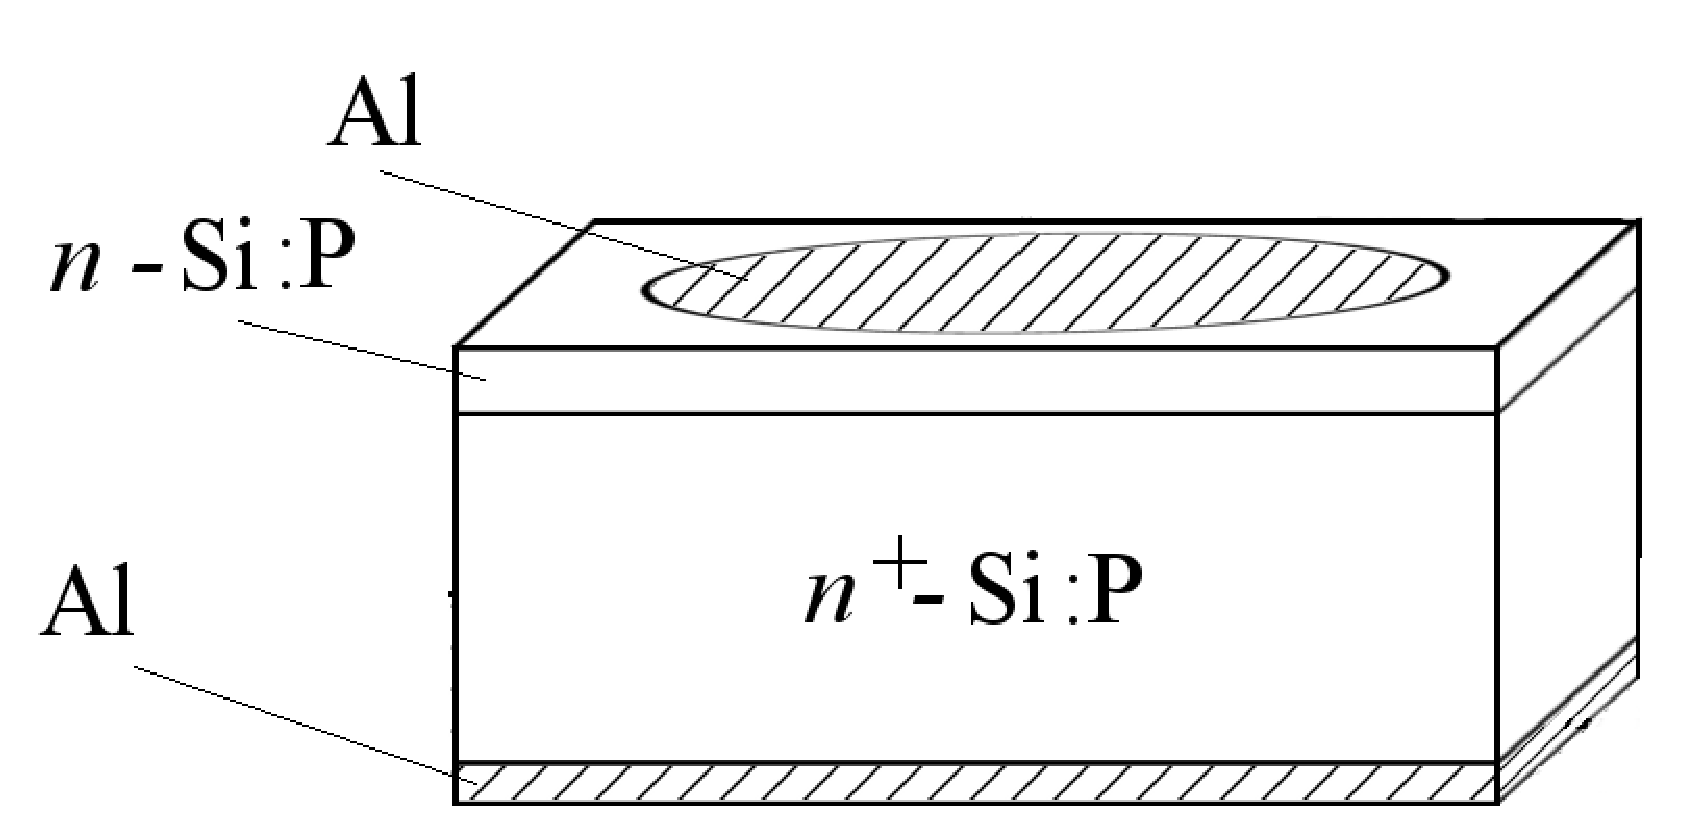
\includegraphics[width=0.65\textwidth]{MSSi}%
\caption{\label{figMSSi}
Структура зразків SSDA.
}
\end{figure}

%Для досліджень використовувалися діоди Шотки з наступною структурою:
%на підкладці $n^+$-Si:Sb (KЭС~0.01, товщина 250~мкм) знаходиться епітаксійний шар $n$-Si:P (товщина 0.2~мкм);
%на поверхні епі-шару створено контакт  Шотки діаметром 2 мм шляхом нанесення шару молібдену;
%на протилежному боці підкладки --- омічний контакт.


В цьому розділі представлені результати дослідження діодів Шотки Al$-n-n^+$--Si---Al,
виготовлених за стандартною технологією \cite{Vorobets:FM2003,StrihaBook1987} на пластинах кремнію КЭФ--1 товщиною $250$~мкм
з орієнтацією (111).
Пластини хімічно очищалися, з неробочої поверхні
повністю видалявся попередньо сформований шар SiO$_2$ для легування фосфором.
На робочій поверхні хімічним травленням створювалися вікна в SiO$_2$ і проводилося очищення
за допомогою іонного пучка.
Потім на робочу поверхню була напилена алюмінієва плівка і проводився процес фотолітографії.
Після цього на протилежну поверхню наносився шар алюмінію товщиною близько 1~мкм і проводився відпал
у інертній атмосфері.
Внаслідок термічної обробки утворювалася структура з випрямляючим контактом на робочій поверхні і омічним на протилежній.

Діаметр контакту Шотки складав 2 мм (площа ДШ $A=3,14\cdot10^{-6}$~м$^2$).
Для контролю рівня легування приповерхневого шару були проведені
вимірювання вольт--фарадних характеристик (ВФХ) досліджуваних структур при кімнатній температурі ($T = 295$~К).
Приклад отриманої залежності наведено на Рис.~\ref{figCV}.
Лінійність залежності $C^{-2}$ від $V$
(де $C$ --- ємність діоду Шотки)
в широкому діапазоні зворотних напруг свідчить про рівномірність легування.
Виявлено, що концентрація носіїв заряду в приповерхневому шарі $N_d\approx1,2\cdot10^{23}$~м$^{-3}$.


\begin{figure}
\center
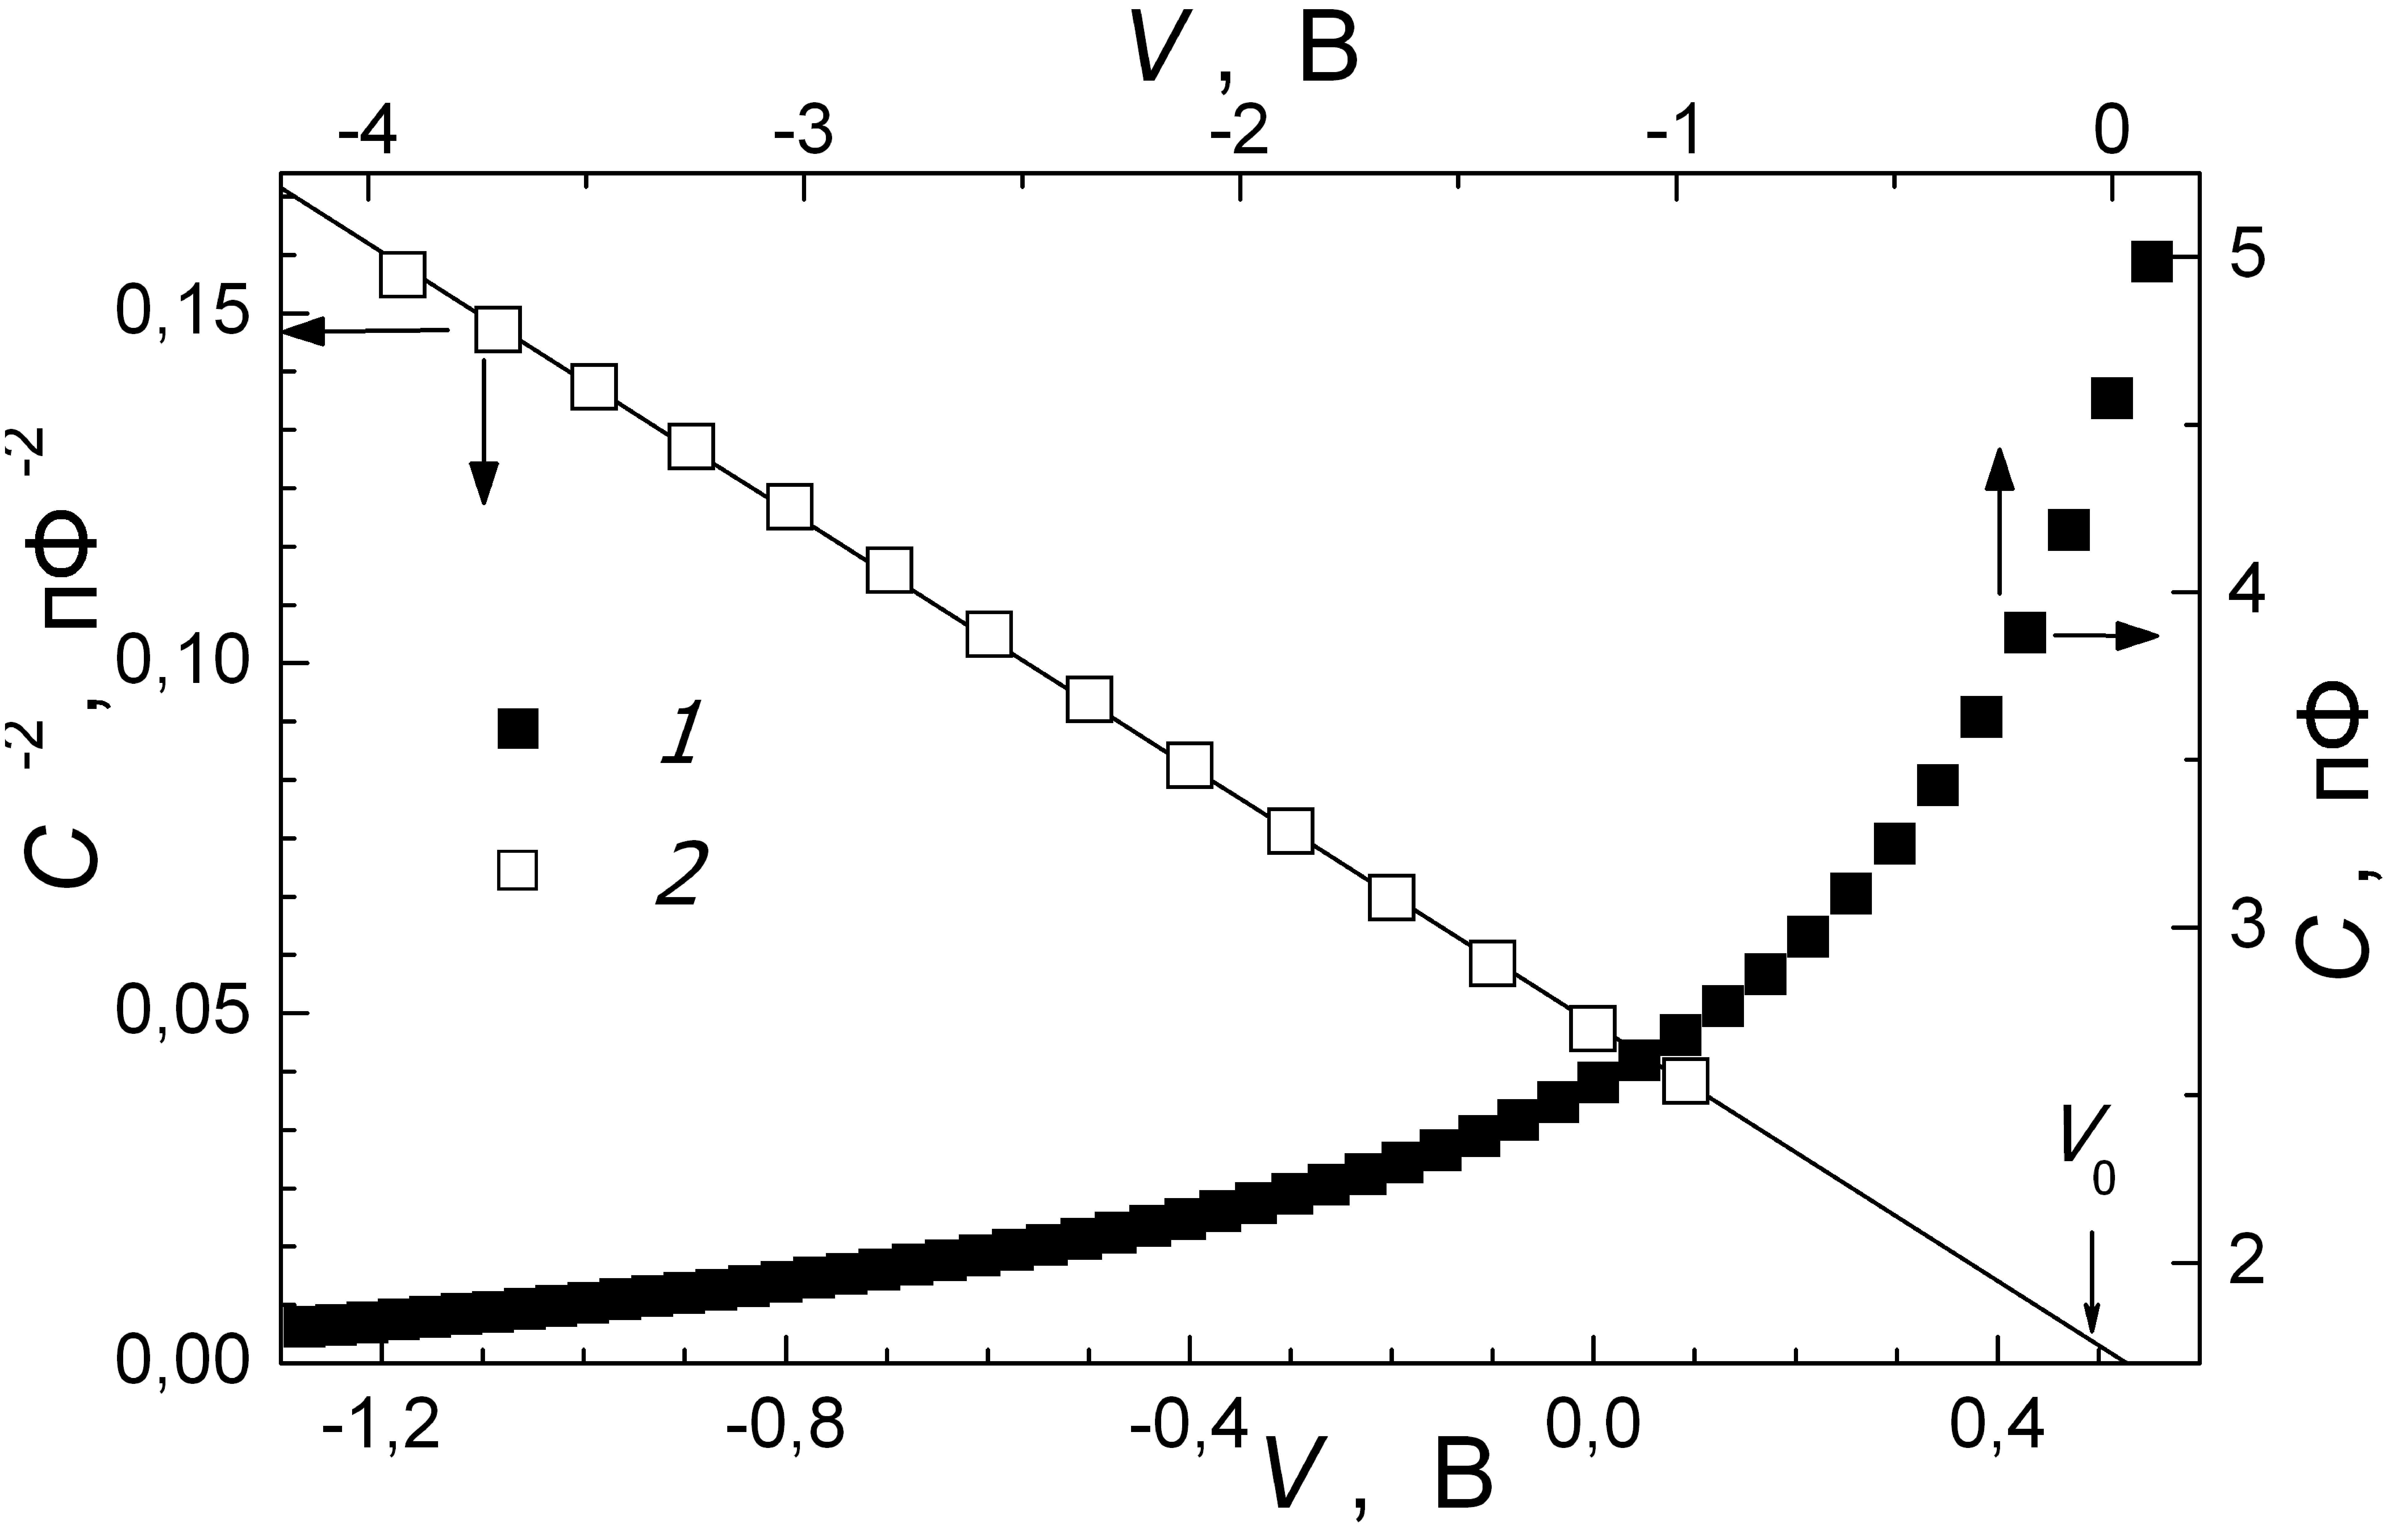
\includegraphics[width=0.7\textwidth]{figCV}
\caption{\label{figCV}
Залежність ємності Al$-n-n^+$--Si---Al діодів Шотки $C$ (крива 1) та величини $C^{-2}$ (2) від прикладеної напруги.
$T=295$~К.
Точки --- експеримент, пряма --- лінійна апроксимація 2.
}%
\end{figure}







%В дисертації представлені результати, отримані з використанням кремнієвих ДШ двох типів,
%які ідентичних за структурою, проте відрізняються концентраціями концентраціями носіїв заряду в епітаксійному шарі $N_d$ та
%підкладці $N_s$, а також площею випрямляючого контакту $A$.
%Для контролю рівня легування були виконані вимірювання вольт--фарадних характеристик (ВФХ) досліджуваних структур при кімнатній температурі ($T = 295$~К).
%Параметри структур, а також їх позначення наведені в Таблиці~\ref{tabMSSi}.




Було проведено вимірювання ВАХ даних структур в діапазоні зміни постійного струму $(10^{-9}\div10^{-2})$~А при
прямому та зворотному зміщенні з кроком по напрузі 0.01~В в діапазоні температур $(130\div330)$~К.


\section{Особливості перенесення заряду в структурах Al$-n-n^+$--Si---Al з бар'єром Шотки\label{MSSi_Non}}
\subsection{Перенесення заряду при прямому зміщенні\label{sbMSSi_NonF}}

%\subsubsection{Особливості аналізу експериментально виміряних ВАХ}

Приклади виміряних прямих ВАХ при різних температурах наведено на рис.~\ref{figIV_SDA}.
Видно, що при температурі більше 250~К прямі ВАХ в напівлогарифмічному масштабі є практично лінійними в інтервалі зміни струму близько трьох порядків.
В той самий час, при $T<210$~K загальний струм можна розділити на дві складові, причому для ВАХ, пов'язаної зі струмом,
який домінує при малих зміщеннях, суттєвим є вплив послідовного опору.
Про це свідчить відхилення від лінійності наведених кривих при при $7\cdot10^{-8}\mbox{A}<I<5\cdot10^{-7}\mbox{A}$.

В літературі \cite{Rhoderick1988,Gromov,Sze2012} показано, що в реальних структурах МН для опису залежності струму від прикладеної прямої напруги
навіть при врахуванні лише термоемісійних процесів замість виразу~(\ref{eqSDIV}) більш доцільно використовувати наступний
\begin{equation}
\label{eqSDIV:2}
I=I_s\exp\left[\frac{q(V-IR_S)}{n_\mathrm{id}kT}\right]\cdot
\left\{1-\exp\left[-\frac{q(V-IR_S)}{kT}\right]\right\}.
\end{equation}
У зв'язку з цим для опису прямих гілок ВАХ було використано вираз
\[
I=I_1+I_2=I_{s1}\exp{\left(\frac{qV}{n_{\mathrm{id},1}kT}\right)}\cdot
\left[1-\exp{\left(-\frac{qV}{kT}\right)}\right]+\]
\begin{equation} \label{eqSDA_IV}
+I_{s2}\exp\left[\frac{q(V-IR_S)}{n_{\mathrm{id},2}kT}\right]\cdot
\left\{1-\exp\left[-\frac{q(V-IR_S)}{kT}\right]\right\},
\end{equation}
де перший доданок $I_1$ є переважаючим при $I>10^{-5}$~A, а другий $I_2$ --- при $I<5\cdot10^{-7}$~A.
Використання двох доданків для опису ВАХ бар'єрних структур широко використовується
в літературі --- див., наприклад, \cite{Arslan,Donoval2010,Huang,GELCZUK2014}.
Зауважимо, що іншим поширеним методом врахування наявності особливостей на ВАХ при малих зміщеннях є введення шунтуючого опору, а не доданку $I_2$.
Проте, на нашу в думку, у даному випадку такий підхід не є виправданим, так як навіть при найменший зміщеннях пряма ділянка ВАХ не є лінійною --- див. вставку на Рис.~\ref{figIV_SDA}.

\begin{figure}
\center
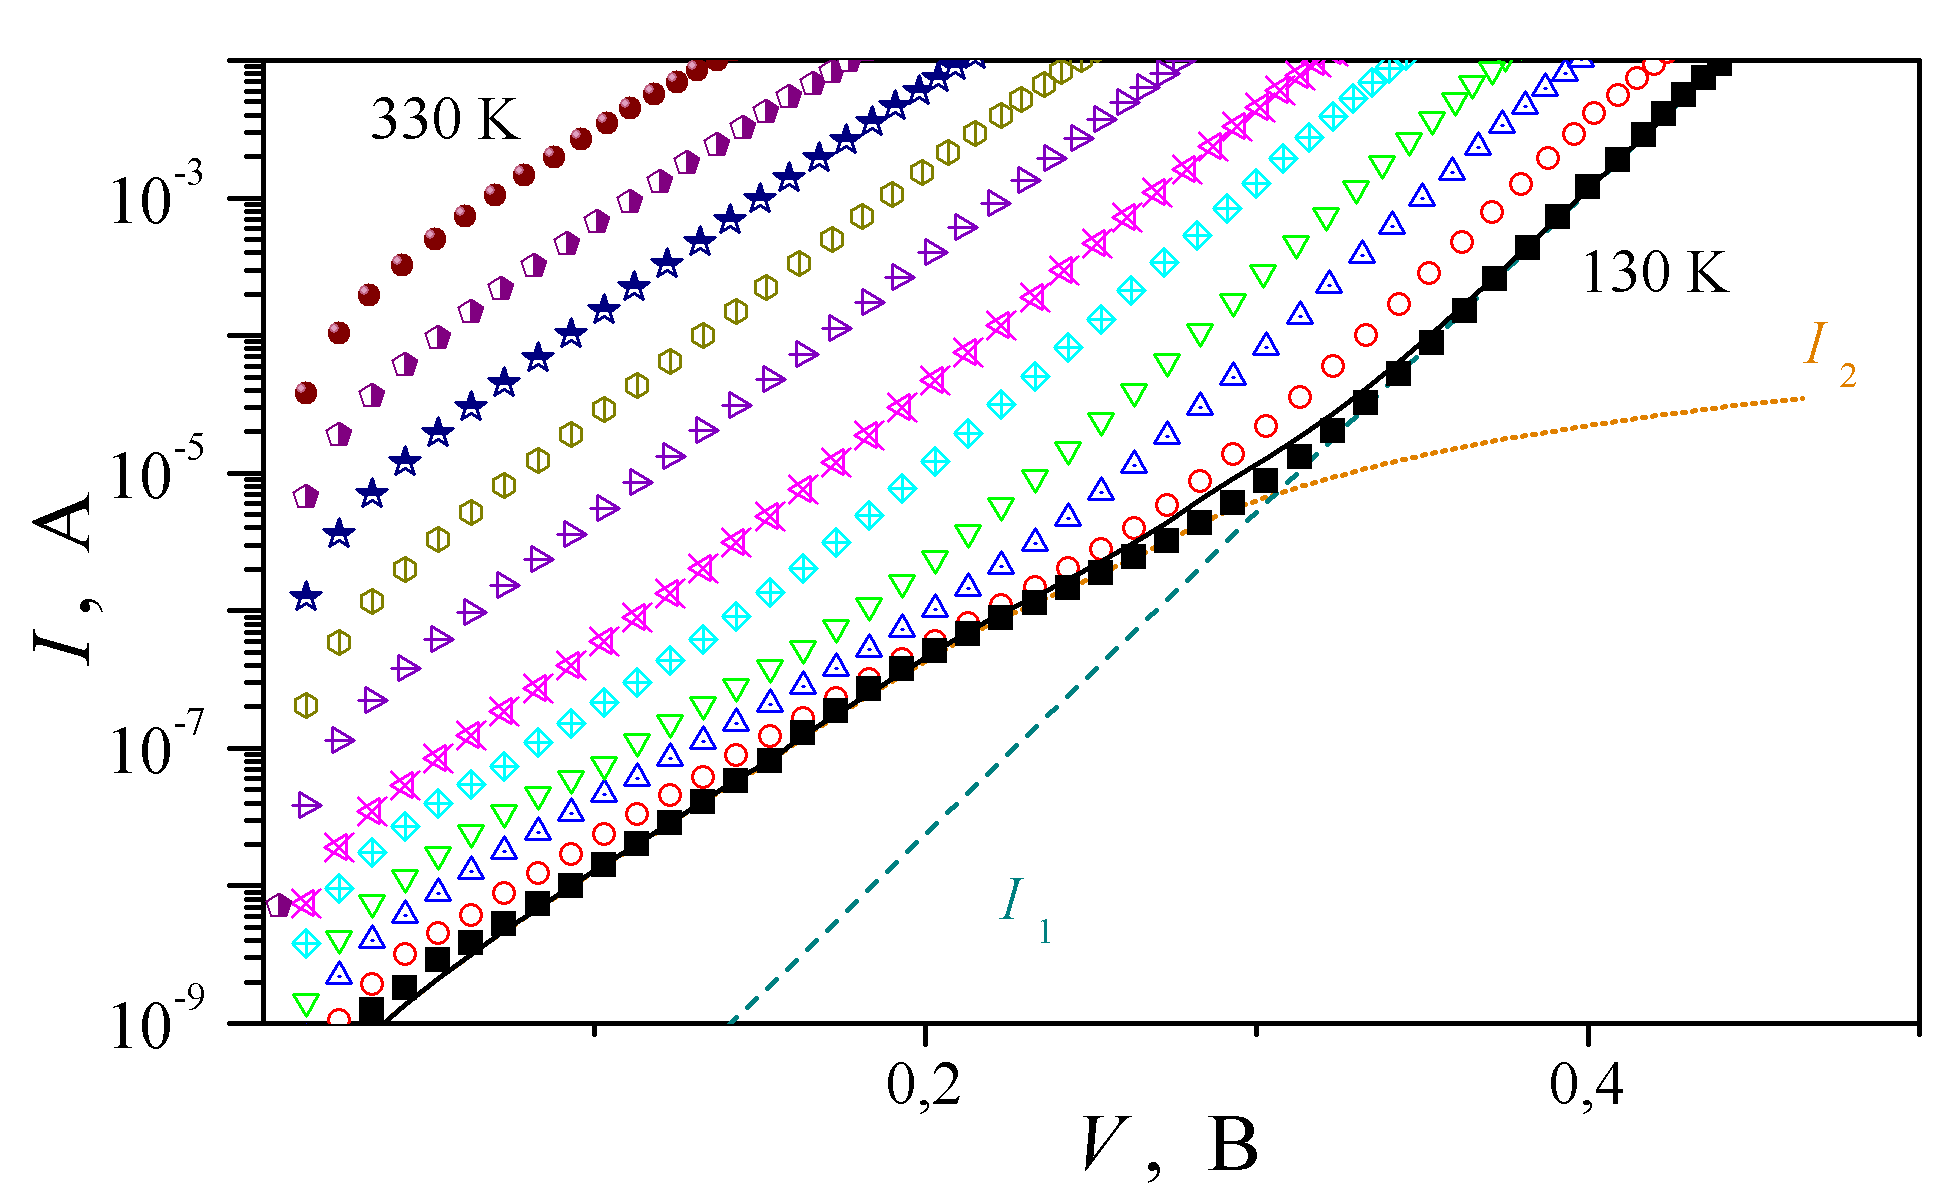
\includegraphics[width=0.8\textwidth]{figIV_SDA}
\caption{\label{figIV_SDA}
Прямі  ділянки ВАХ структур SSDA в температурному діапазоні $130\div330$~К.
Наведено криві, виміряні з кроком 20~К.
Лінії --- апроксимація прямої ВАХ при $T=130$~К за формулою~(\ref{eqSDA_IV}):
штрихова -- струм $I_1$, пунктирна -- $I_2$,
суцільна -- їх сума;
параметри апроксимації $n_{\mathrm{id},1}=1,67$,
$n_{\mathrm{id},2}=2,53$,
$I_{s1}=5,0\cdot10^{-13}$~A,
$I_{s2}=3,8\cdot10^{-10}$~A, $R_{s}=4.1\cdot10^3$~Ом.
На вставці --- початкова ділянка прямої ВАХ при $T=130$~K.
}%
\end{figure}

Для визначення апроксимаційних параметрів використовувалася наступна процедура.
Пряма ВАХ розбивалася на дві ділянки,
для яких $10^{-5}\mbox{A}<I<10^{-2}\mbox{A}$ та
$10^{-9}\mbox{A}<I<10^{-7}\mbox{A}$.
Використовуючи дані першої, виконувалась побудова залежності величини $\ln{{I}/{\left[1-\exp\left(-qV/kT\right)\right]}}$ від $V$, яка надалі
апроксимувалася за методом найменших квадратів прямою,
кутовий коефіцієнт та вільний член якої пов'язані з $n_{\mathrm{id},1}$ та $I_{s1}$ відповідно.
Спираючись на дані другої ділянки ВАХ і використовуючи методи Cheung \cite{Cheung} та Gromov \cite{Gromov}, визначалась величина $R_s$.
Використання двох методів мало на меті підвищити достовірність отриманих даних і воно показало, що отримані обома шляхами значення близькі (в межах 10\%) між собою.
Після визначення $R_s$, будувалась залежність $\ln (I /\{1 - \exp[ -q (V - IR_s) / (kT ) ]\})$ від
ефективної напруги $(V-IR_s)$ і для знаходження $I_{s2}$ та $n_{\mathrm{id},2}$ використовувалася процедура, описана вище.

На рис.~\ref{figIV_SDA} наведено приклад апроксимації експериментальної прямої ВАХ при одній з температур за формулою \eqref{eqSDA_IV} з використанням параметрів,
отриманих за описаною методою.
Видно задовільний збіг розрахованої кривої та експериментальних точок.

У випадку, коли проходження струму через бар'єр визначається ТЕ, то висота бар'єру Шотки при
нульовому зміщенні $\Phi_b$ пов'язана зі струмом насичення співвідношенням \cite{Rhoderick1988}:
\begin{equation}
\label{eqFb:TE}
\Phi_b=\left(\frac{kT}{q}\right)\cdot\ln\left(\frac{AA^*T^2}{I_s}\right).
\end{equation}
Отримані температурні залежності для висот бар'єрів та факторів неідеальності обох компонент струму наведено на Рис.~\ref{figFbT_SDA}.

%Розглянемо спочатку особливості струму, переважаючого при високих температурах та великих зміщеннях ($I_1$).


\begin{figure}
\center
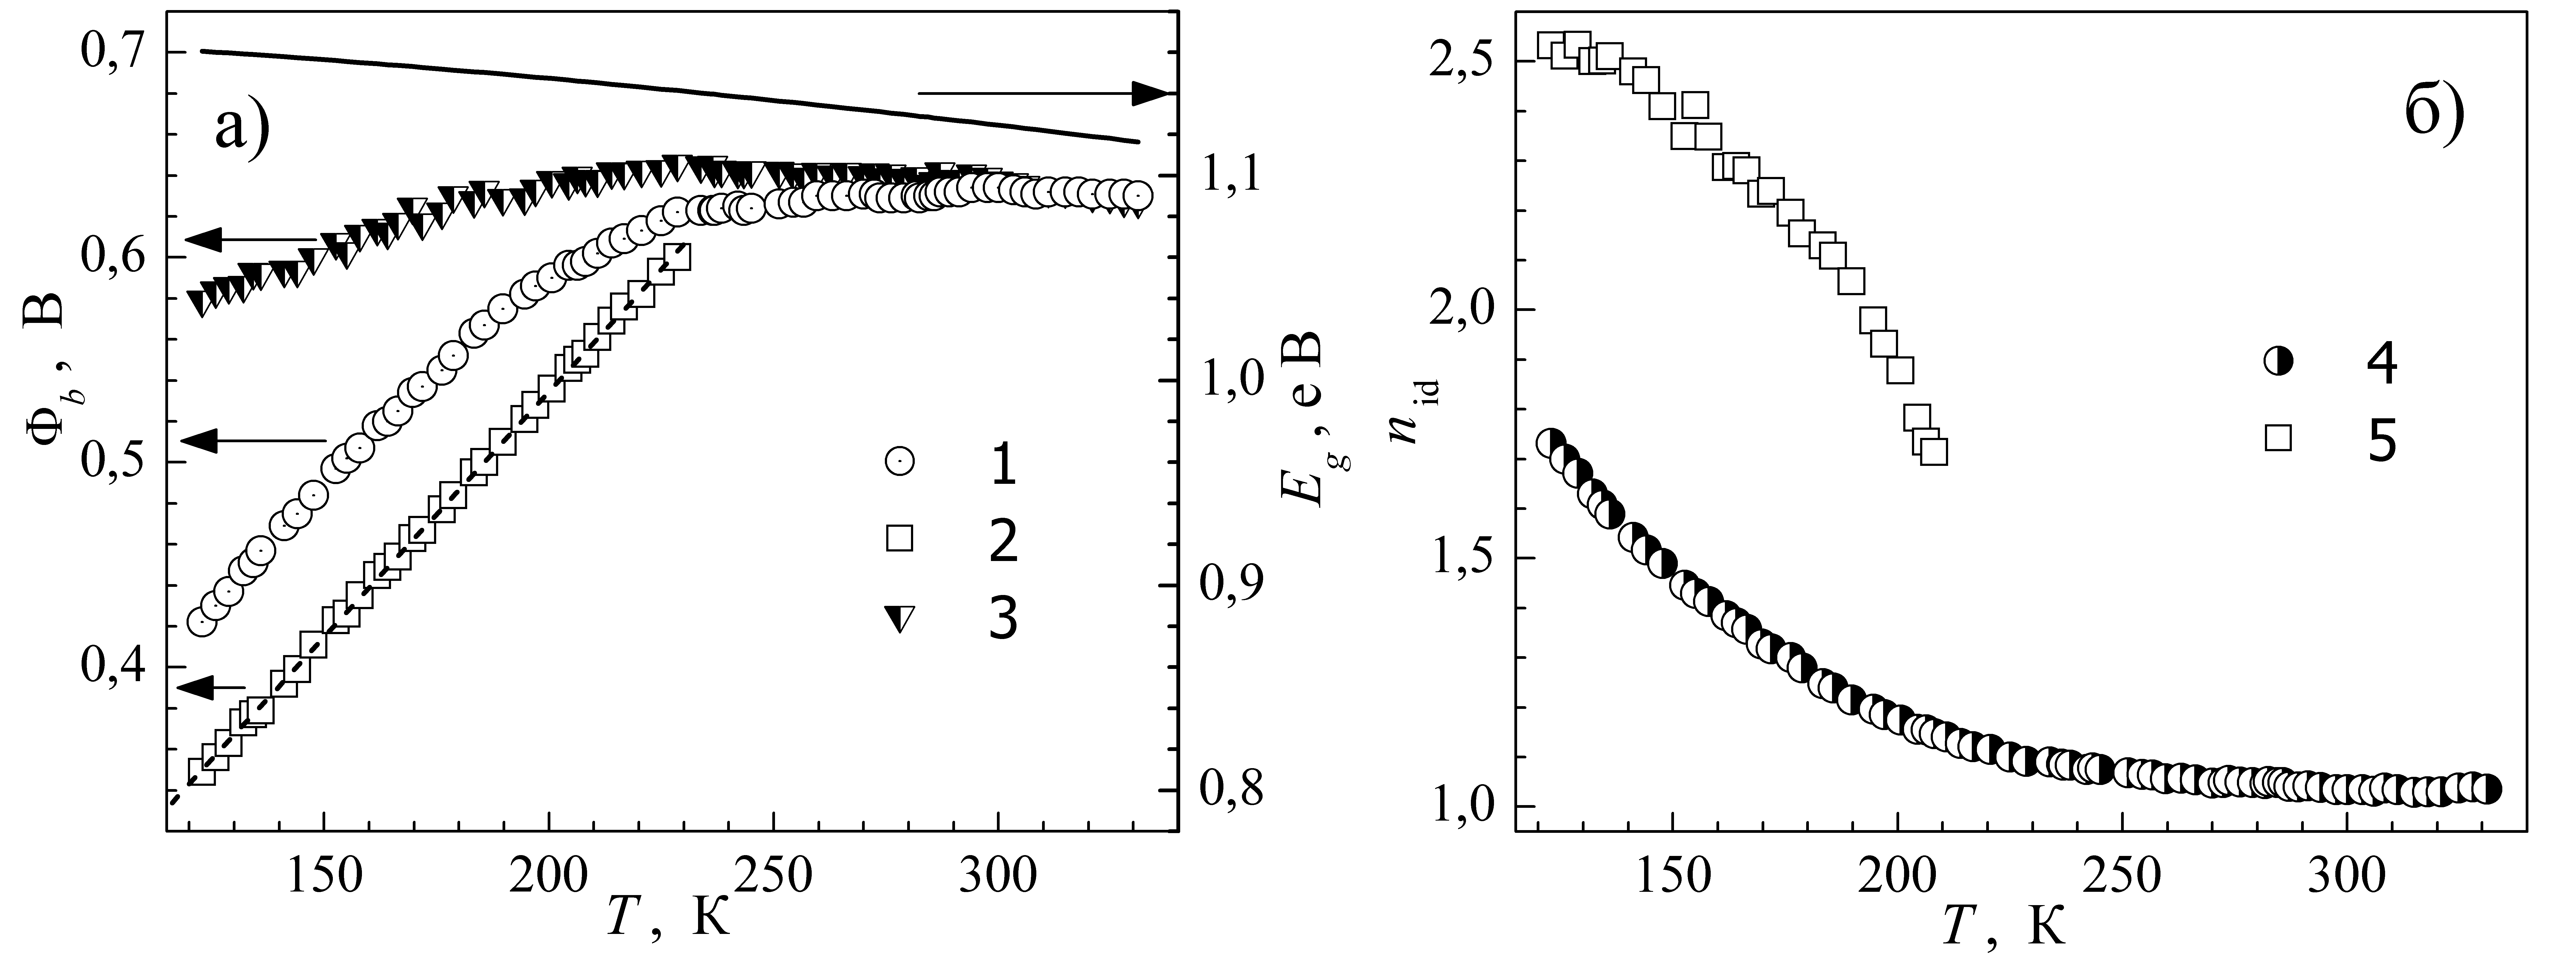
\includegraphics[width=0.5\textwidth]{figFbT_SDA}
\caption{\label{figFbT_SDA}
Температурні залежності висоти бар'єру (а) та фактору неідеальності (б) структури SSDA.
1 -- $\Phi_{b1}$,
2 -- $\Phi_{b2}$,
3 -- $\Phi_{b1}^\mathrm{eff}$ ,
4 -- $n_{\mathrm{id},1}$, 5 -- $n_{\mathrm{id},2}$.
Пунктир -- лінійна апроксимація кривої 2.
Також приведено температурну залежність ширини забороненої зони Si (а, суцільна лінія).
}%
\end{figure}

З рисунка видно, що при збільшенні температури фактор неідеальності зменшується, наближаючись
до одиниці при кімнатних температурах.
Як відомо, що температурна залежність фактору неідеальності залежить від механізму перенесення заряду.
Зокрема, для ідеального випадку ТЕ очікується, що $n_{\mathrm{id}}=1$ при будь--яких температурах.
Проте для реальних контактів така рівність не спостерігається і для опису залежності $n_{\mathrm{id}}(T)$
часто використовують вираз \cite{Rhoderick1988, Sze2012}
\begin{equation}\label{eqN_T:TE}
n_{\mathrm{id}}=1+\frac{T_0}{T},
\end{equation}
де $T_0$ --- певна константа, що не залежить від температури та зміщення в широкому температурному інтервалі.

Проте залежність, подібна до зображеної на Рис.~\ref{figFbT_SDA},б очікується
і у випадку, коли домінуючим механізмом є термопольова  емісія (ТПЕ), польова емісія (ПЕ) або тунелювання за участю глибоких рівнів (DAT)
\cite{Rhoderick1988,Evstropov,Soylu,JYOTHI2015,OZAVCI2013,Abhishek}.
В цьому випадку
\begin{equation}\label{eqN_T:TFE}
n_{\mathrm{id}}^\mathrm{T}=\frac{E_{00}}{kT}\cdot\coth\left(\frac{E_{00}}{kT}\right),
\end{equation}
де $E_{00}$ --- характеристична енергія тунелювання.


\begin{figure}
\center
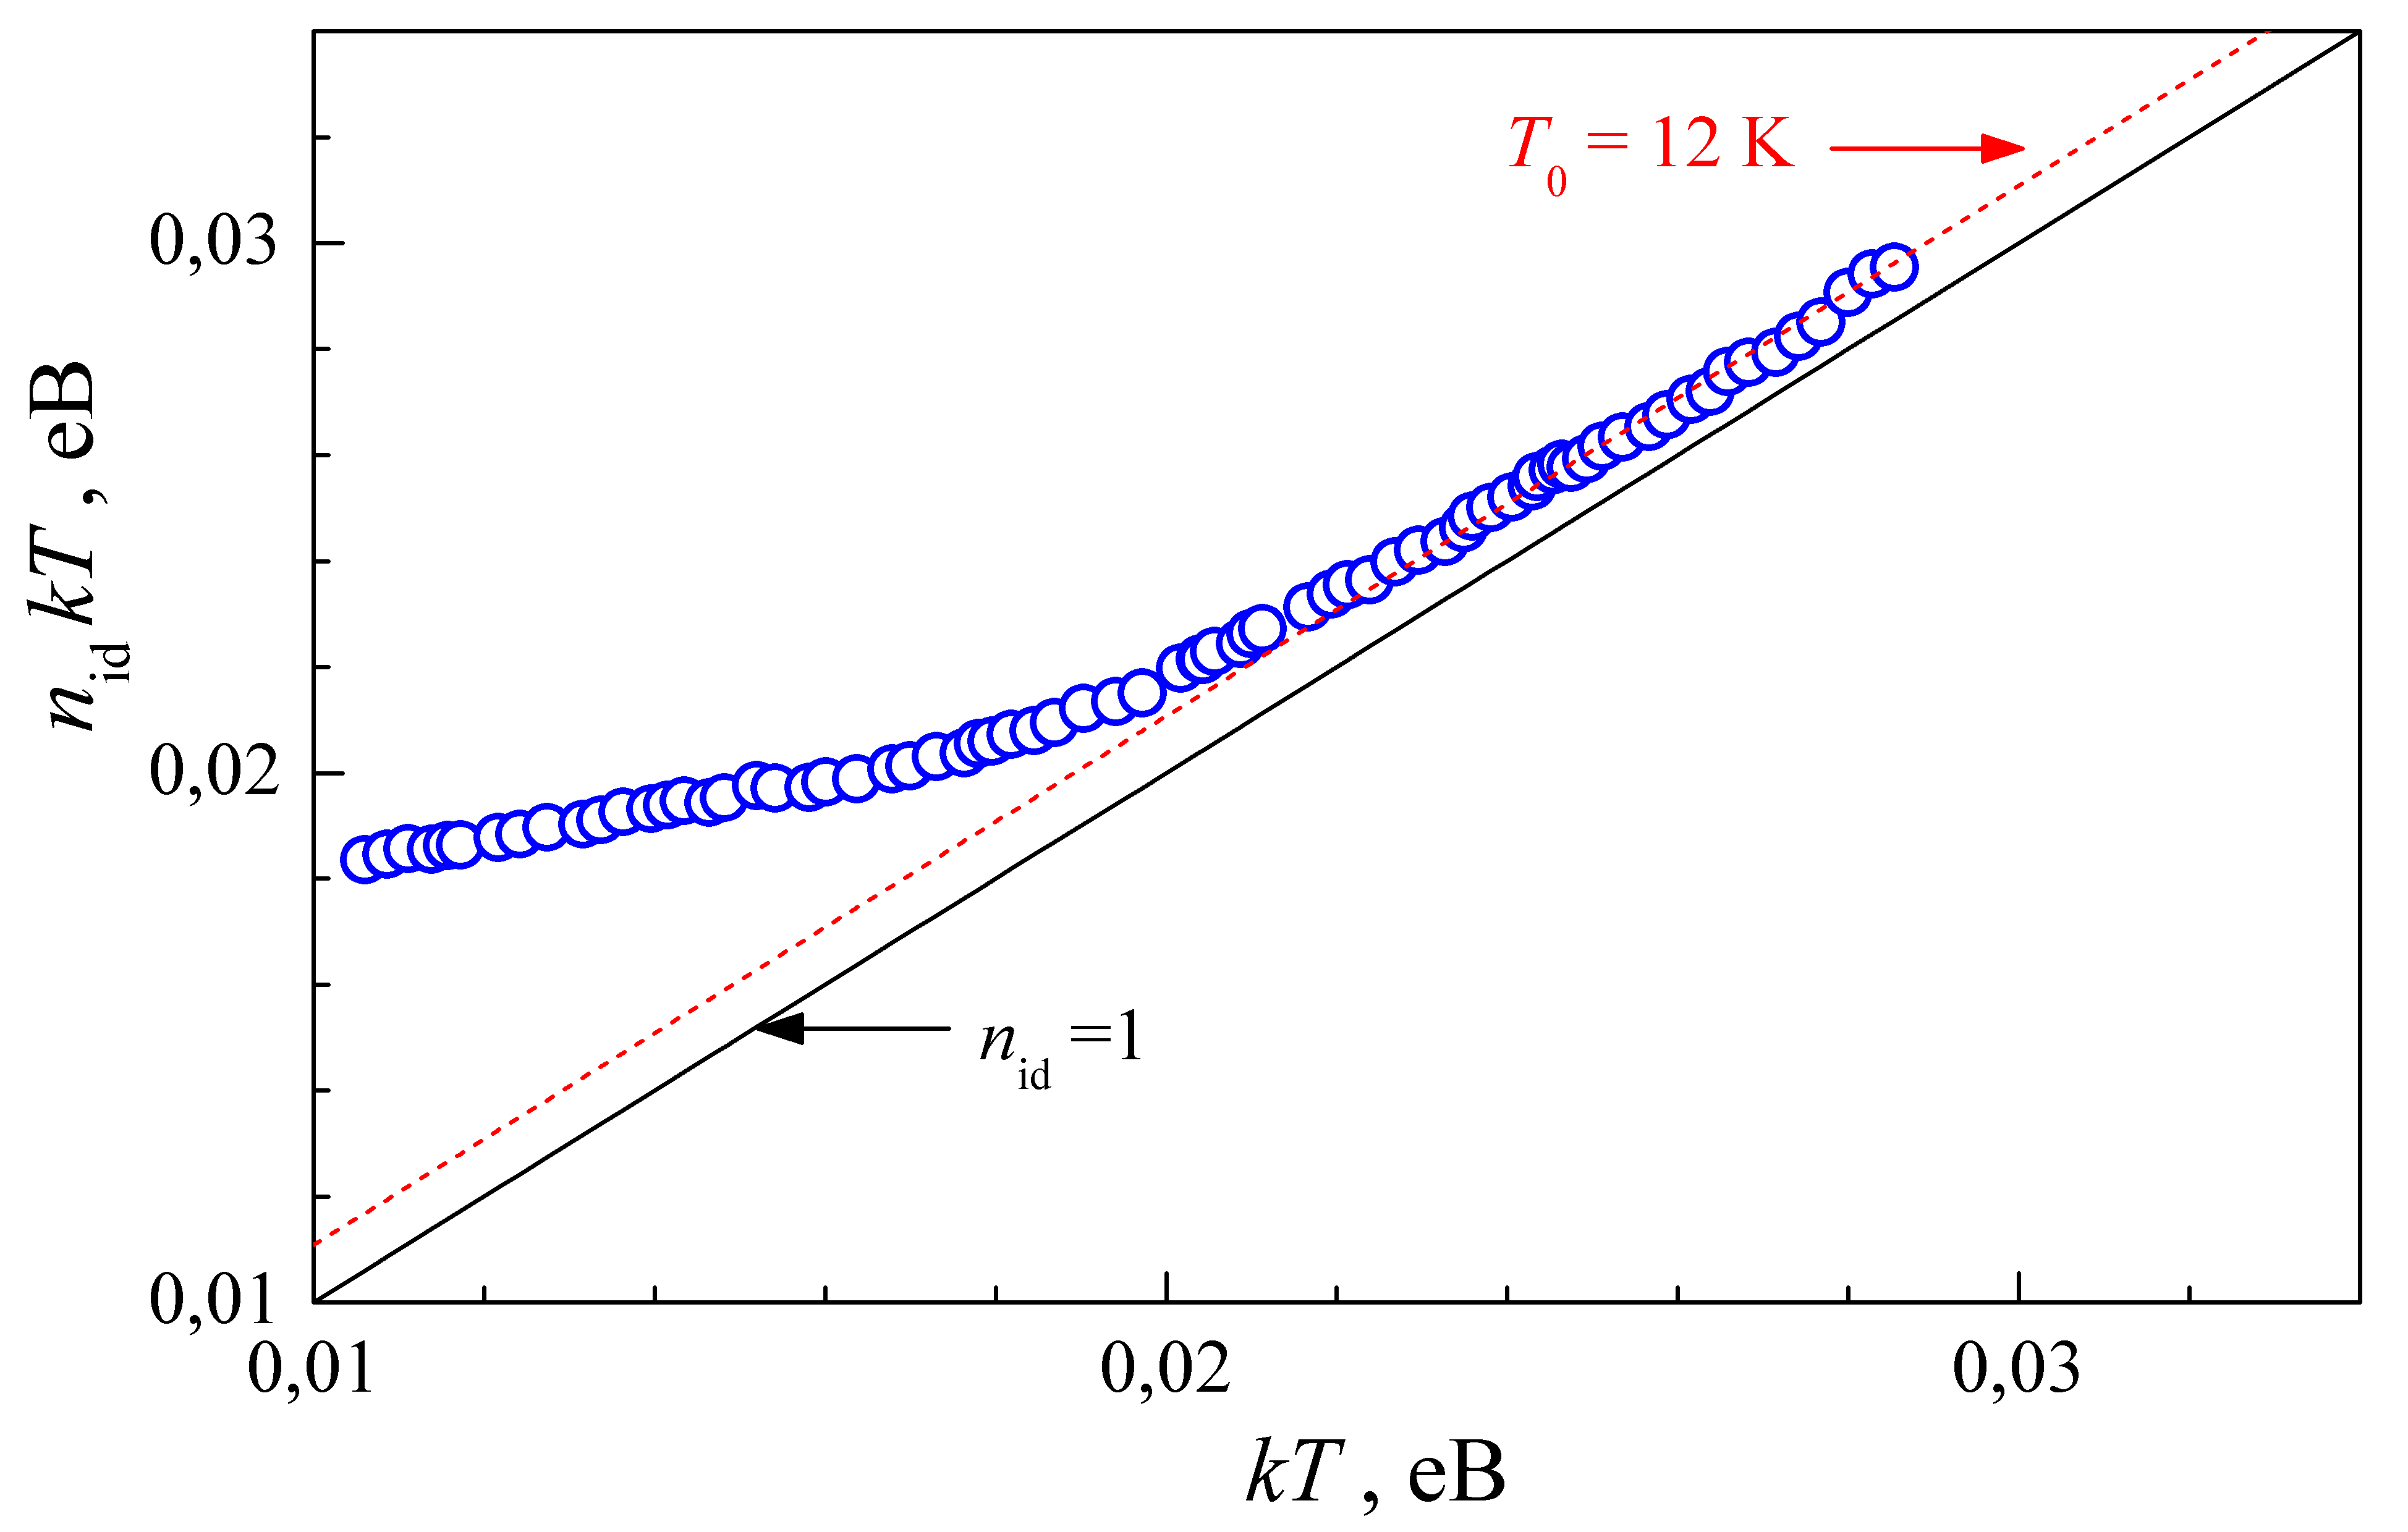
\includegraphics[width=0.75\textwidth]{figNT_SDA}
\caption{\label{figNT_SDA}
Температурна залежність оберненого нахилу ВАХ.
1 --- $n_{\mathrm{id},1}$;
2 --- $n_{\mathrm{id},2}$.
Пунктир --- теоретичні криві відповідно до формул (\ref{eqN_T:TE}) (криві А та В)
та (\ref{eqN_T:TFE}) (криві С-G).
$T_0$, K: 12 (A), 206 (B).
$E_{00}$, мВ: 12 (С), 17 (D), 22 (E), 27 (F), 32 (G).
Також наведено ідеальний випадок ($n_{\mathrm{id}}=1$) --- пряма суцільна лінія.
}%
\end{figure}

На Рис.~\ref{figNT_SDA} наведено експериментально отримані залежності факторів неідеальності від оберненої температури
для обох струмових компонент та декілька кривих, розрахованих з використанням виразів (\ref{eqN_T:TE}) та (\ref{eqN_T:TFE}).
Видно, що отримані дані для $n_{\mathrm{id},1}$ (при $T>220$~K) та $n_{\mathrm{id},2}$ задовільно описуються
виразом (\ref{eqN_T:TE}) при $T_0=12$~К та $T_0=206$~К, відповідно,
що свідчить на користь ТЕ як основного механізму перенесення заряду.
Зауважимо, що при ТПЕ
\begin{equation}\label{eqE00:TFE}
E_{00}^\mathrm{TFE}=\frac{\hbar}{2}\sqrt{\frac{N_d}{m^*\varepsilon_s\varepsilon_0}},
\end{equation}
($m^*$ -- ефективна маса електрону, $m^*=1.08\cdot9.11\cdot10^{-31}$~кг)
і тому для досліджених зразків та температурного діапазону очікувалось, що при домінуванні цього механізму $n\approx1$.



Раніше вже згадувалося, для однорідного контакту Шотки теоретично \cite{Rhoderick1988} та експериментально \cite{Aboelfotoh,Zhua} показано,
що при підвищенні температури за умови домінування термоелектронної емісії ВБШ має зменшуватися,
причому температурні коефіцієнти змін $\Phi_b$ та  $E_g$ дуже близькі між собою.
На Рис.~\ref{figFbT_SDA},а також наведена температурна залежність $E_g$, розрахована з використанням
виразу (\ref{eqEg}).
Для дослідженої структури спостерігається зворотна тенденція: ВБШ зі збільшенням температури зростає практично у всьому
діапазоні
і лише для компоненти $I_1$ поблизу кімнатної температури поведінка $\Phi_b$ нагадує $E_g$.

З іншого боку, відомо, що ВБШ, визначена за допомогою ВАХ, може відрізнятися від реальної.
Зокрема, в роботі \cite{Bozhkov} стверджується про необхідність проведення вимірів при сталому струмі через контакт
і пропонується для оцінки ефективної висоти бар'єру $\Phi_{b}^\mathrm{eff}$ використовувати вираз
\begin{equation}\label{eqBoz}
\Phi_{b}^\mathrm{eff}=n_{Ic}\Phi_b-(n_{Ic}-1)\cdot\frac{kT}{q}\cdot\ln\left(\frac{AA^*T^2}{I_c}\right),
\end{equation}
де
$n_{Ic}$ --- фактор неідеальності при певному сталому значенні струму $I_c$.
В роботі \cite{Bozhkov} також показано, що у випадку ТЕ через однорідний контакт $\Phi_{b}^\mathrm{eff}$ майже збігається за величиною
з реальною висотою бар'єру і має з нею однакову температурну залежність.

Результати обчислення $\Phi_{b1}^\mathrm{eff}$ для $I_{s1}$ згідно з формулою (\ref{eqBoz}) при $I_c=10^{-3}$~А показані на Рис.~\ref{figFbT_SDA}, крива 3.
Видно, що хоча величина $\Phi_{b1}^\mathrm{eff}$ і змінюється в значно меншому діапазоні,
проте її температурна залежність також відрізняється від поведінки $E_g$, особливо при низьких температурах.


Якщо ТЕ є домінуючим механізмом перенесення заряду, то параметр $A^*$ може бути
визначений \cite{Rhoderick1988,Schroder2006} шляхом побудови так званої залежності Річардсона,
тобто залежності величини $\ln(I_s/T^2)$ від $(kT)^{-1}$.
Згідно з (\ref{eqFb:TE}), вона має описуватися виразом
\begin{equation}\label{eqRich}
\ln\left(\frac{I_s}{T^2}\right)=\ln(AA^*)-\frac{q\Phi_b}{kT},
\end{equation}
тобто залежність Річардсона має бути прямою, нахил якої визначається ВБШ,
я точка перетину з вертикальною віссю --- константою $A^*$.


Відповідна залежність, побудована для даних, отриманих для складової $I_1$ наведена
на Рис.~\ref{figRich_SDA}, крива 1.
Видно, що лінійна залежність дійсно спостерігається, але не у всьому діапазоні температур, а у двох окремих піддіапазонах.
Шляхом апроксимації в діапазоні $(130\div220)$~К були отримані значення $3,7\cdot10^{-10}$~А$\cdot$см$^{-2}\cdot$К$^{-2}$ та
$0,141$~В для сталої Річардсона та висоти бар'єру, відповідно,
тоді як для діапазону $(230\div330)$~К ---
$30$~А$\cdot$см$^{-2}\cdot$К$^{-2}$ та $0,599$~В.
Величини також наведені в Таблиці~\ref{tabPar:SSDA}.
Очевидно, що отримані значення сталої Річардсона суттєво відрізняються від літературних даних
для кремнію (112~А$\cdot$см$^{-2}\cdot$К$^{-2}$).


\begin{figure}
\center
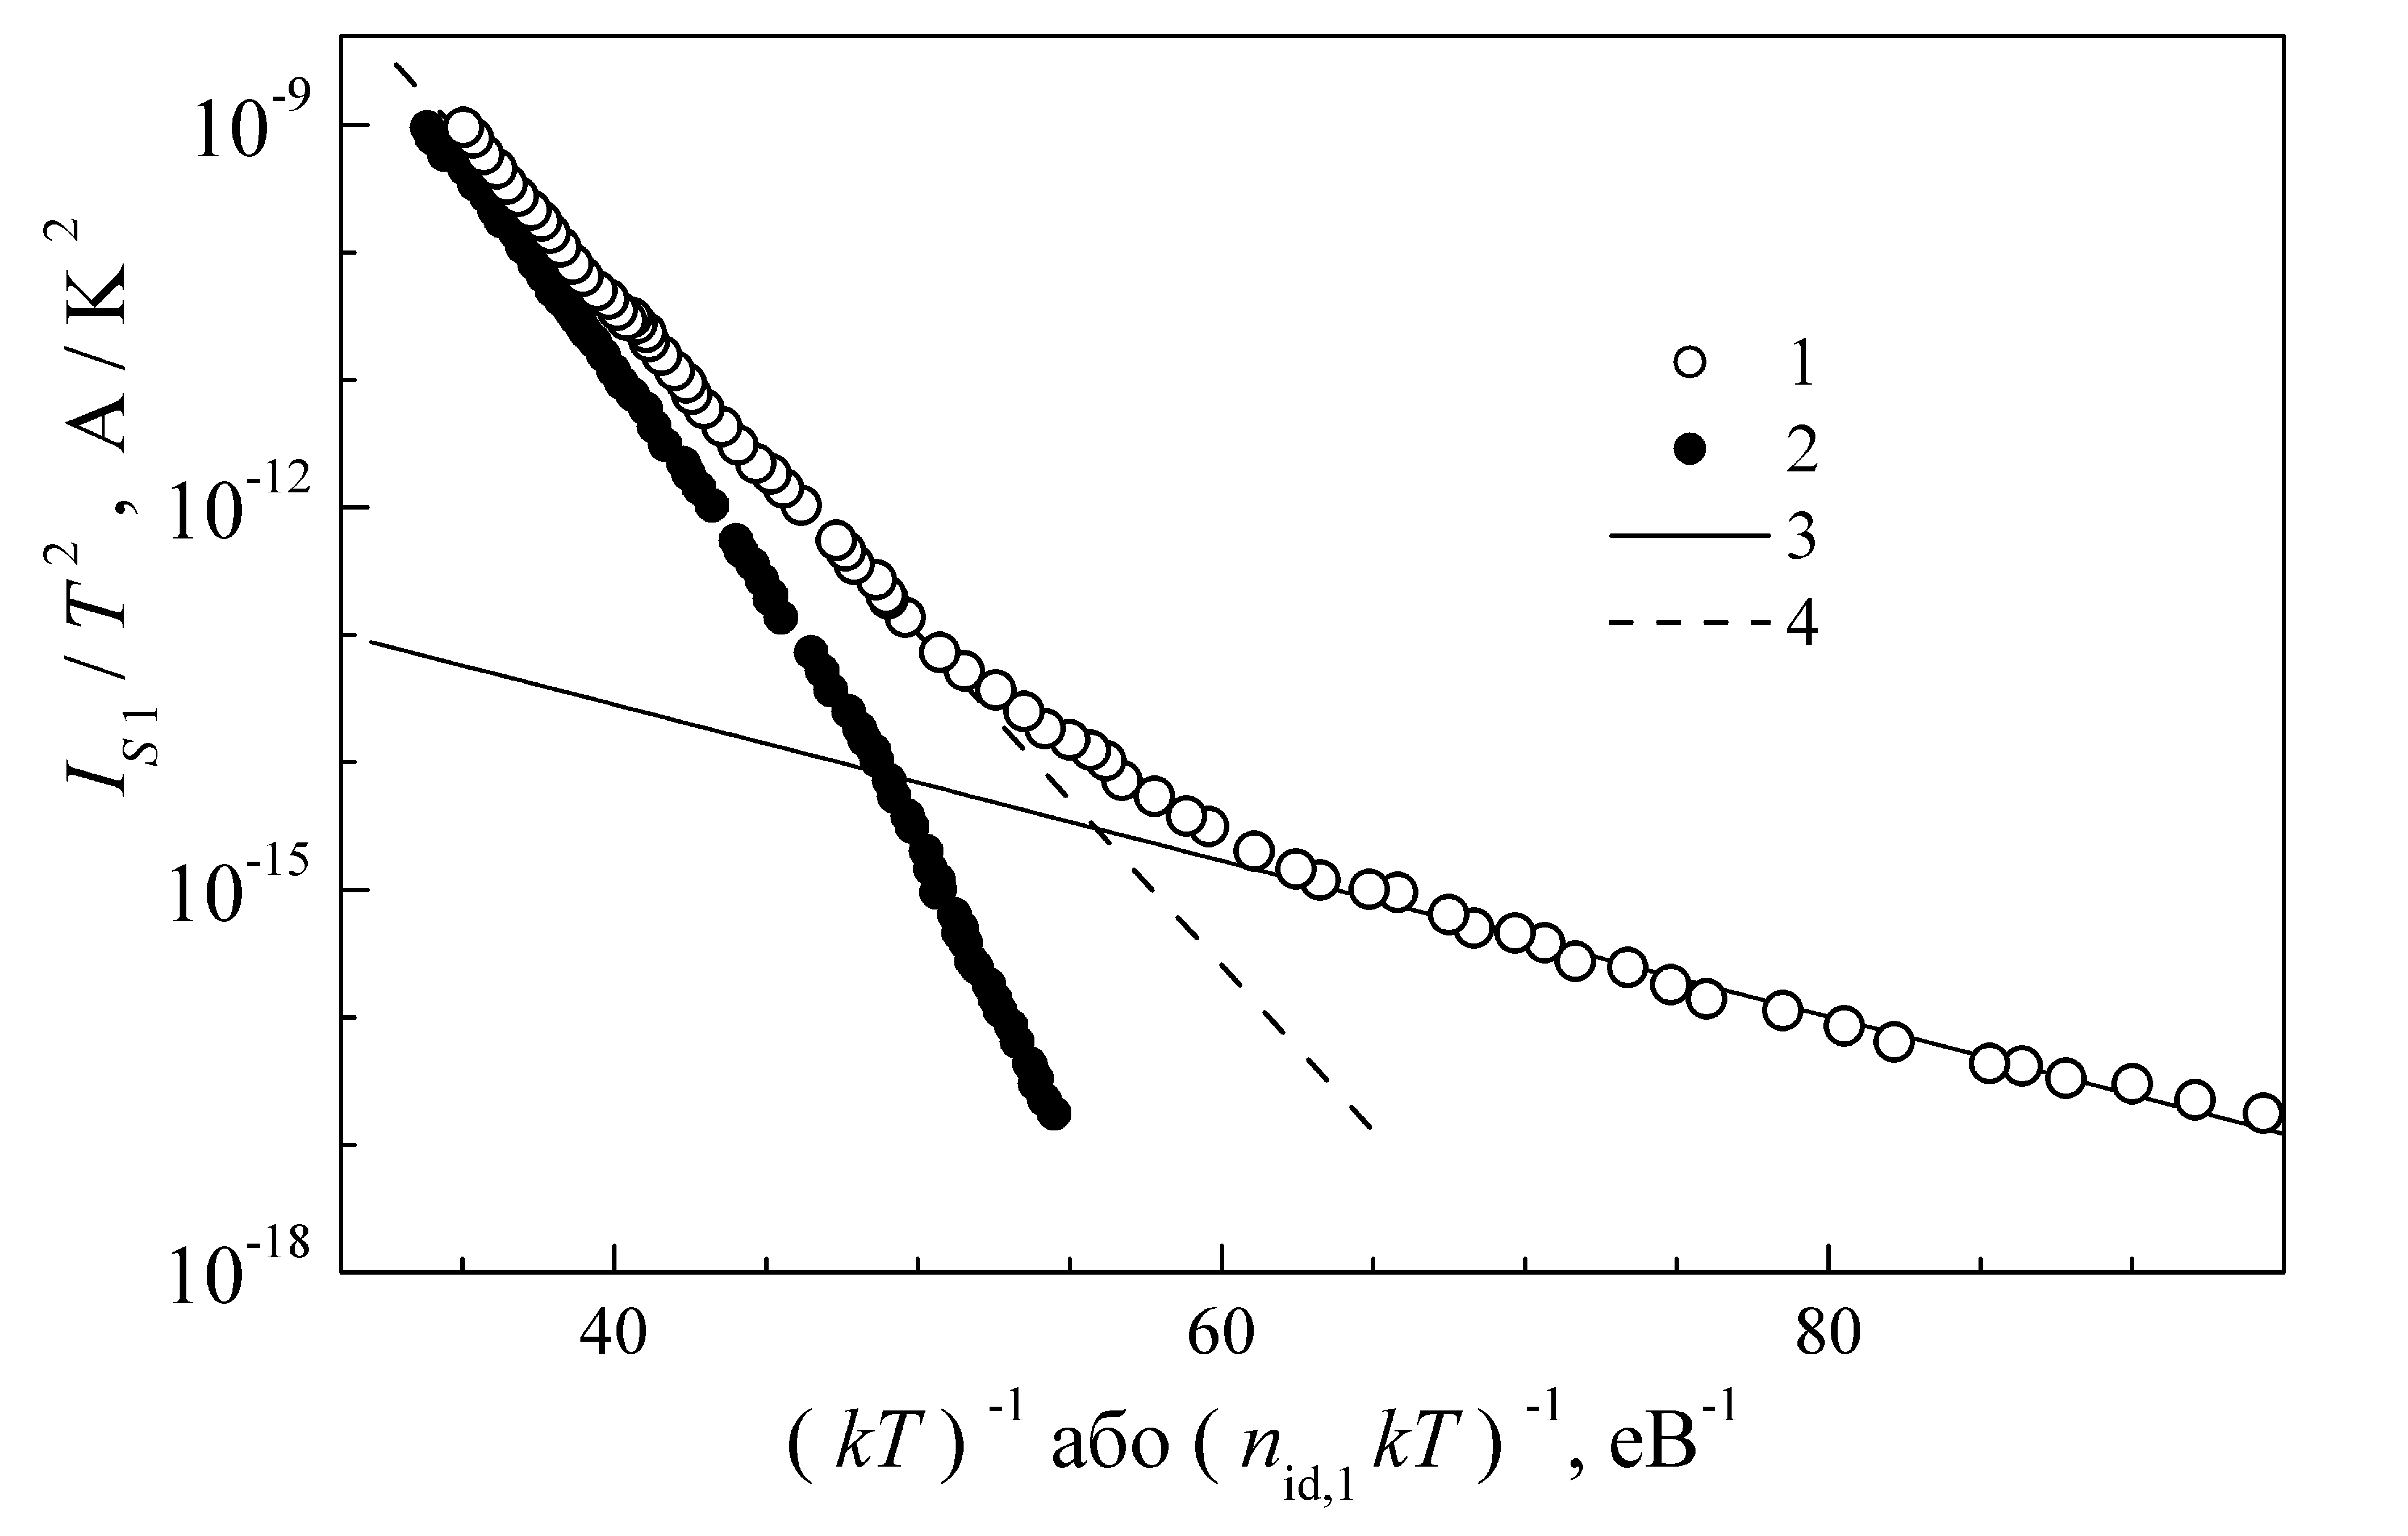
\includegraphics[width=0.7\textwidth]{figRich_SDA}
\caption{\label{figRich_SDA}
Залежності Річардсона, побудовані для високотемпературної компоненти струму $I_1$
за формулами (\ref{eqRich}) (крива 1) та (\ref{eqRichB}) (крива 2).
Прямі --- лінійна апроксимація даних кривої 1 в діапазонах $T=(130\div220)$~К (3, суцільна)
та $T=(230\div330)$~К (4, пунктир).
}%
\end{figure}



\begin{table}
\caption{\label{tabPar:SSDA}Параметри, визначені для високотемпературної складової струму неопромінених структур SSDA.
}
\center
\begin{tabular}{|l|c|c|}
\hline
\multicolumn{1}{|c|}{Параметр:}& \multicolumn{2}{c|}{Температурний інтервал}\\ \cline{2-3}
метод визначення&$130\div220$~K&$230\div330$~K\\
\hline
%$A^*_R$, А$\cdot$см$^{-2}\cdot$К$^{-2}$&$3.7\cdot10^{-10}$&32\\ \hline
\multicolumn{1}{|c|}{$A^*$, А$\cdot$см$^{-2}\cdot$К$^{-2}$:}&&\\
залежність Річардсона (\ref{eqRich})&$(3,7\pm0,8)\cdot10^{-10}$&$32\pm10$\\
видозмінена залежність Річардсона (\ref{eqRichB})&$(3,0\pm0,6)\cdot10^{8}$&$40\pm8$\\
модифікована залежність Річардсона (\ref{eqRich:Mod})&$122\pm20$&$112\pm8$\\
література  \cite{Schroder2006}& \multicolumn{2}{c|}{$\,\,\,\,\,\,\,\,\,\,\,\,$   112}\\ \hline
\multicolumn{1}{|c|}{$\Phi_b$, мВ:}&&\\
залежність Річардсона (\ref{eqRich})&141$\pm$4&599$\pm$3\\
видозмінена залежність Річардсона (\ref{eqRichB})&1090$\pm$10&751$\pm$5\\
залежність $\Phi_b=f(\frac{1}{2kT})$&872$\pm$4&663$\pm$3\\
залежність $\Phi_b=f(n_\mathrm{id})$&646$\pm$5&640$\pm$20\\
модифікована залежність Річардсона (\ref{eqRich:Mod})&872$\pm$3&662$\pm$3\\
ВФХ &&683$\pm$2\\
\hline
залежність $\Phi_b=f(\frac{1}{2kT})$:&&\\
\multicolumn{1}{|c|}{$\sigma_{\Phi0}$, мВ} &99$\pm$1&40$\pm$5\\
\multicolumn{1}{|c|}{$\rho_2$, $10^{-2}$} &33$\pm$1&12$\pm$1\\
\multicolumn{1}{|c|}{$\rho_3$, мВ }&17,0$\pm$0,3&8,0$\pm$0,3\\
\hline
\end{tabular}
\end{table}



У роботі \cite{Aldemir} показано, що
У випадку суттєвого відхилення від ідеальності (величина $n_\mathrm{id}$ значно більша за одиницю)
для визначення $A^*$ можна також використовувати \cite{Aldemir,Mohan} видозмінену залежність Річардсона,
відкладаючи по осі абсцис не $(kT)^{-1}$, а $(n_\mathrm{id} kT)^{-1}$:
\begin{equation}\label{eqRichB}
\ln\left(\frac{I_s}{T^2}\right)=\ln(AA^*)-\frac{q\Phi_b}{n_\mathrm{id}kT},
\end{equation}
Проте для нашого випадку і видозмінена залежність Річардсона (Рис.~\ref{figRich_SDA}, крива 2) не є лінійною для всього
температурного діапазону, а отримані значення $A^*$ (див. Таблицю~\ref{tabPar:SSDA}) суттєво відрізняються
від табличних.

Узагальнюючи вищенаведене, необхідно визнати, що отримані результати неможливо пояснити з точки зору теорії ТЕ через однорідний контакт.


З іншого боку, відмінності між експериментально виявленою температурною залежністю ВБШ та очікуваною теоретично нерідко
пов'язують із неоднорідністю границі розділу між металом та напівпровідником \cite{Dokme}.
Впливу неоднорідності можна позбутися розглядаючи ВБШ за умови плоских зон (<<flat band condition>>) $\Phi_{b}^\mathrm{FB}$:
\begin{equation}
\label{eqFbfb}
\Phi_{b}^\mathrm{FB}=n_\mathrm{id}\Phi_{b}-(n_\mathrm{id}-1)V_n\,,
\end{equation}
де
\begin{equation}
\label{eqVn}
qV_n=kT\ln\left(\frac{N_c}{N_d}\right)
\end{equation}
різниця енергій між дном зони провідності та положенням рівня Фермі в об'ємі напівпровідника,
так званий <<bulk potential>>.
На Рис.~\ref{figFbfb_SDA} наведена температурна залежність $\Phi_{b}^\mathrm{FB}$, розрахована для високотемпературної компоненти $I_1$.
Зауважимо, що на рисунку також наведена температурна залежність ширини забороненої зони, причому
масштаби осей $\Phi_{b}^\mathrm{FB}$ та $E_g$ однакові.
З рисунка видно, що поведінка ВБШ в наближенні плоских зон та ширини забороненої зони дуже подібні,
що свідчить про те, що механізмом перенесення заряду в досліджуваних структурах може бути ТЕ через неоднорідний бар'єр.


\begin{figure}
\center
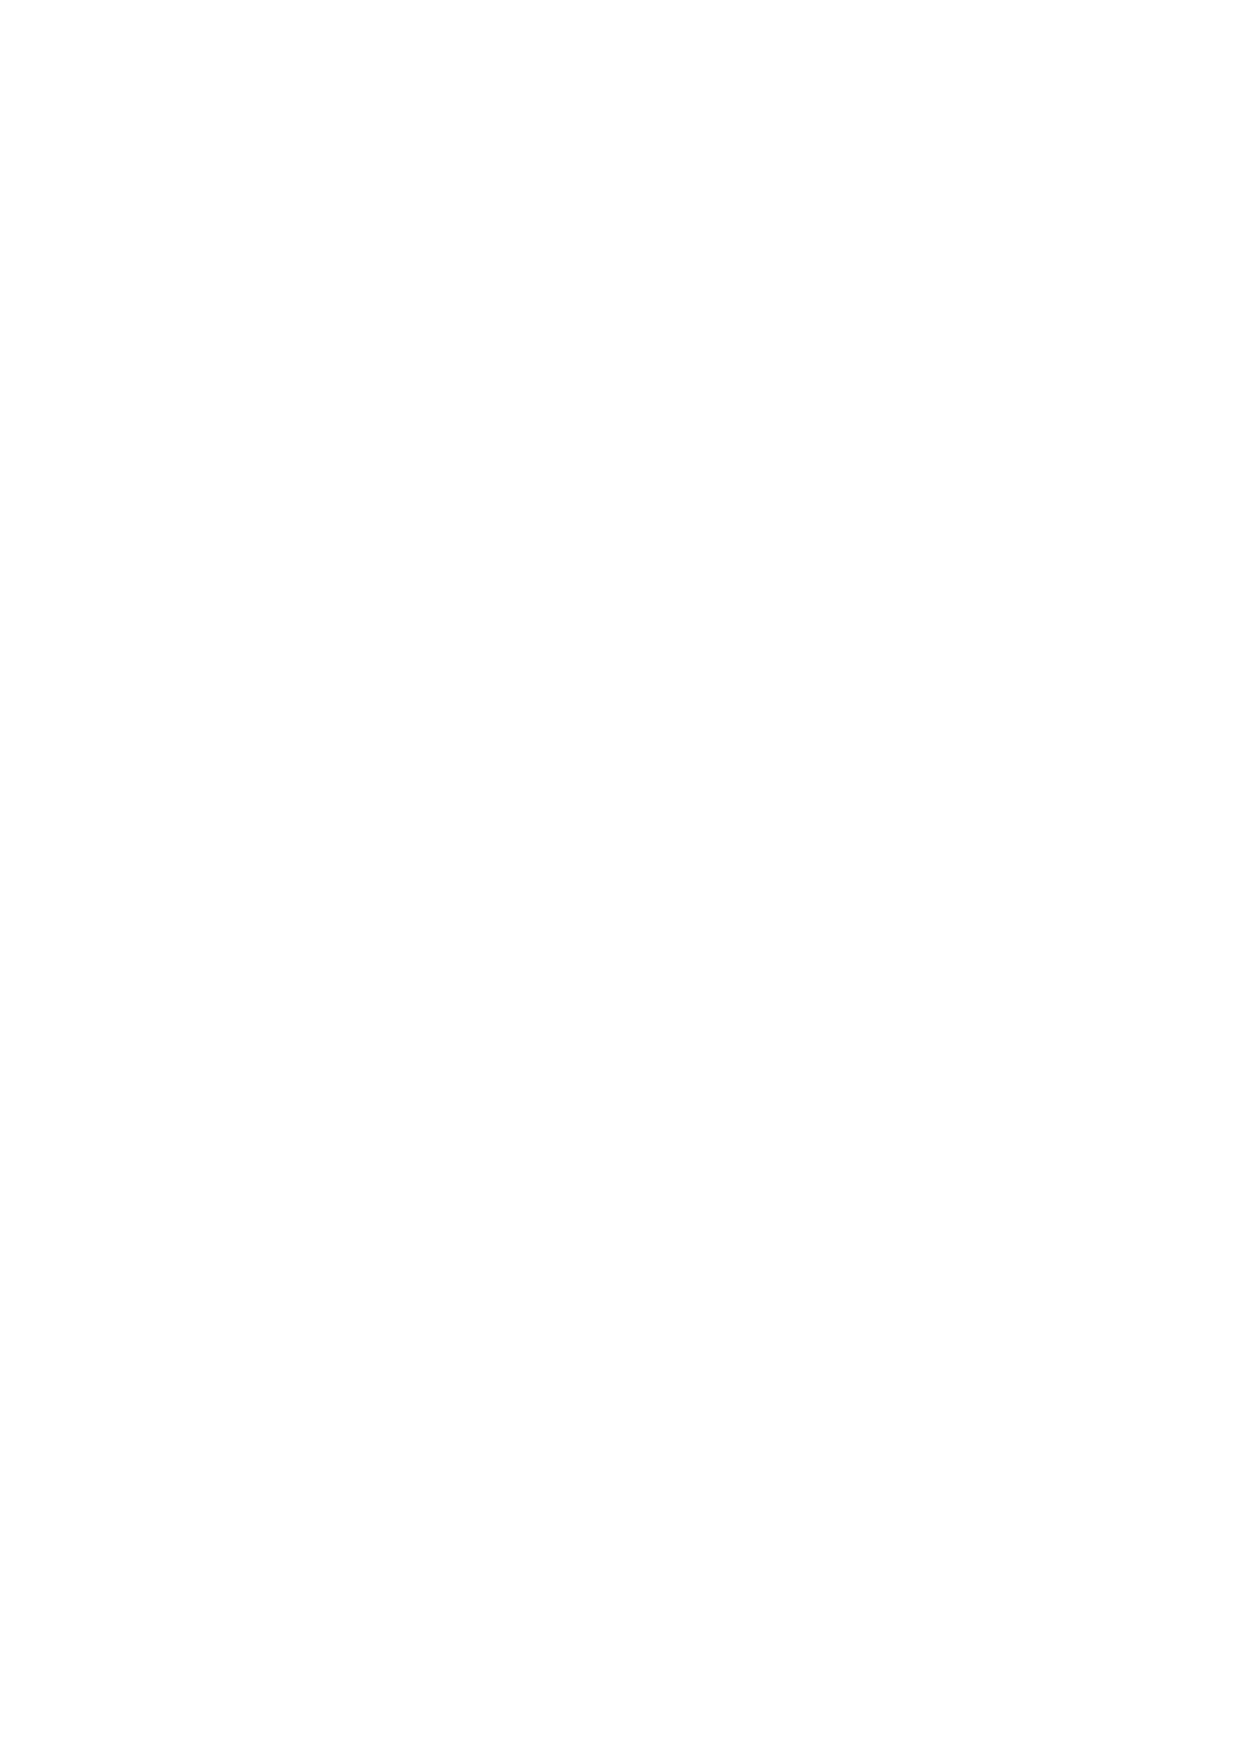
\includegraphics[width=0.7\textwidth]{figFbfb_SDA}
\caption{\label{figFbfb_SDA}
Температурні залежності ВБШ в наближені плоских зон (точки, права вісь), розрахованої
для високотемпературної компоненти струму $I_1$, та ширина забороненої зони (пунктир, ліва вісь).
}%
\end{figure}

В літературі для пояснення експериментально отриманих ВАХ структур МН використовуються два
підходи \cite{Sarpatwari, Tascioglu2010, Yildirim2010, Mamor, Iucolano2007JAP, Iucolano2007APL}, які дозволяють
%\cite{Sarpatwari, Aydemir, Turut, Mamor, Iucolano, Iucolano2}.
врахувати неоднорідність бар'ру Шотки,
схематично ілюстровані за допомогою Рис.~\ref{figFbModel}.
Згідно з першим підходом, запропонованим в \cite{Werner}, вважається, що контакт між металом та напівпровідником
змінюються від точки до точки (Рис.~\ref{figFbModel},а),  просторовий розподіл ВБШ  може бути описаний розподілом Гауса:
\begin{equation}\label{eqFbWerner}
  P(\Phi_{b}^j)=\frac{1}{\sigma_\Phi\sqrt{2\pi}}\exp\left[-\frac{(\Phi_{b}^j-\overline{\Phi}_{b})^2}{2\sigma_\Phi^2}\right]\,,
\end{equation}
де
$P(\Phi_{b}^j)$ --- ймовірність того, що значення висоти бар'єру в певній точці дорівнює $\Phi_{b}^j$,
$\overline{\Phi}_{b}$ --- середнє значення ВБШ,
$\sigma_\Phi$ --- стандартне відхилення висоти бар'єру, показник однорідності контакту.
Також вважається, що $\overline{\Phi}_{b}$ та $\sigma_\Phi$ залежать
від прикладеної напруги і польова залежність може бути описана лінійними функціями
\begin{equation}\label{eqFbV}
   \overline{\Phi}_{b}(V)=\Phi_{b}^0+\rho_2\,V\,,
\end{equation}
\begin{equation}\label{eqNV}
   \sigma_\Phi^2(V)=\sigma_{\Phi0}^2+\rho_3\,V\,,
\end{equation}
де
$\Phi_{b}^0$ та $\sigma_{\Phi0}$ відповідають нульовому зміщенню,
а коефіцієнти $\rho_2$ та $\rho_3$ описують зміну розподілу ВБШ при прикладанні напруги.

\begin{figure}
\center
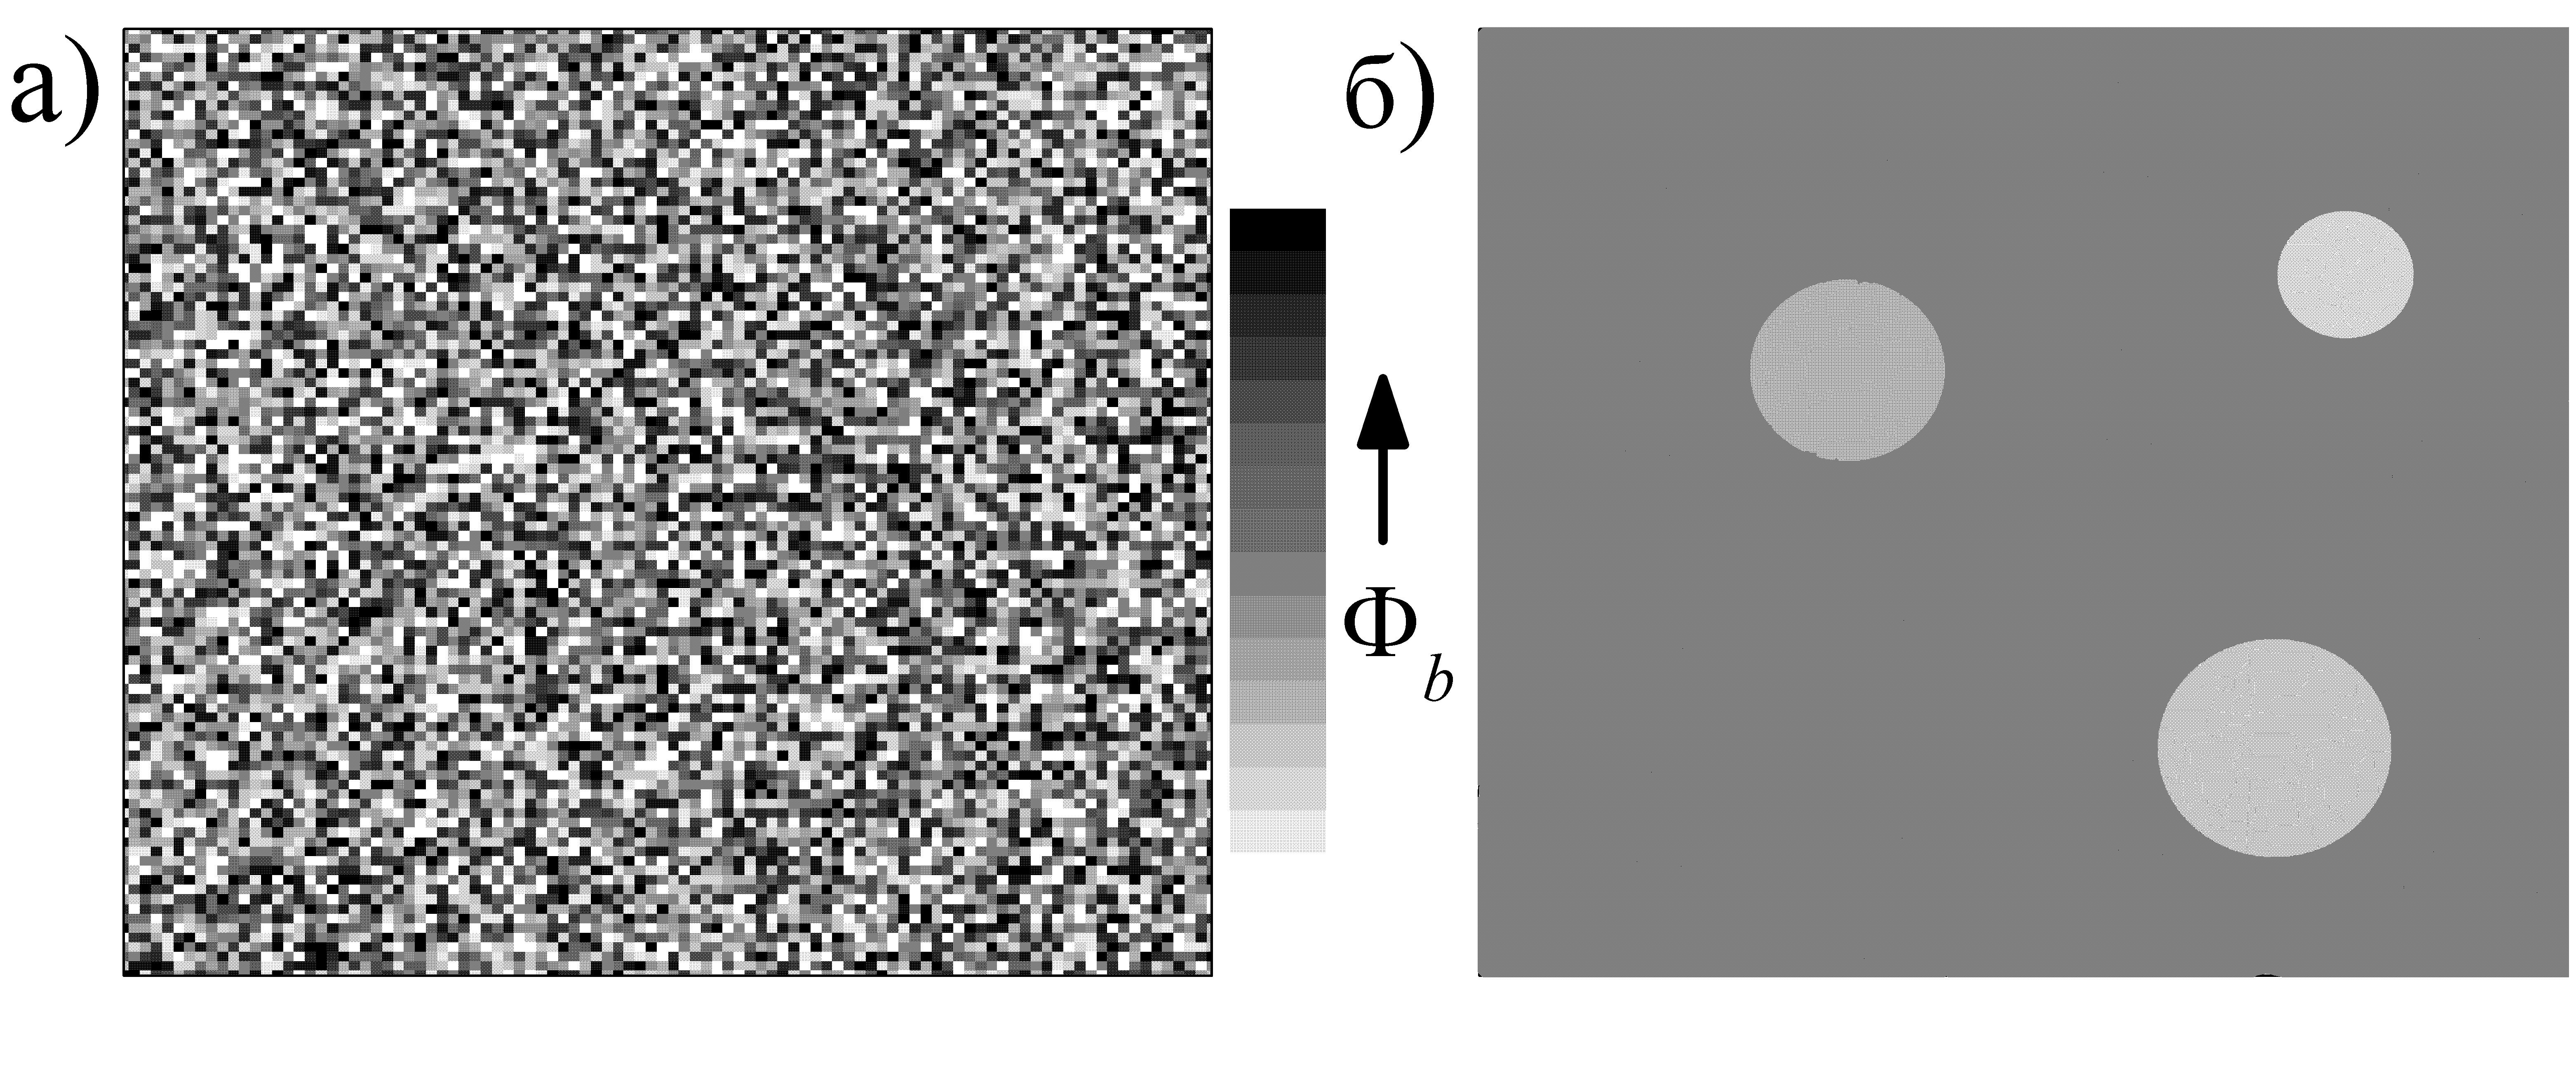
\includegraphics[width=0.9\textwidth]{figFbModel}
\caption{\label{figFbModel}
Моделі неоднорідного по площі контакту МН:
а --- ВБШ визначається розподілом Гауса;
б --- однорідний бар'єр з патчами.
}%
\end{figure}

Ця теорія передбачає,
що фактор неідеальності, який визначається за нахилом ВАХ, і ВБШ, розрахована за допомогою виразу (\ref{eqFb:TE}),
пов'язані з $\rho_2$ та $\rho_3$ і
$\Phi_{b}^0$ та $\sigma_{\Phi0}$, відповідно \cite{Werner,Tascioglu2010,Yildirim2010,Mamor,Soylu}:
\begin{equation}\label{eqNidT}
  \frac{1}{n_\mathrm{id}}-1=\rho_2+\frac{q\rho_3}{2kT}\,,
\end{equation}
\begin{equation}\label{eqFb0T}
\Phi_b=\Phi_b^0-\frac{q\sigma^2_{\Phi0}}{2kT}.
\end{equation}

Відповідно до іншої моделі неоднорідного контакту Шотки \cite{Sullivan,Tung:PhysRev,Tung:MSE,Tung:ApplPhysRev}, ВБШ вважається однаковою на всій границі МН,
окрім невеликих за площею ділянок (так званих патчів), де значення ВБШ менше --- Рис.~\ref{figFbModel},б.
Ділянки можуть відрізнятися між собою площею та висотою бар'єру, причому відповідний характерний параметр описується розподілом Гауса.

В ряді робіт \cite{Iucolano2007JAP, Iucolano2007APL} показано, що ці теорії можуть бути використані сумісно,
причому за наявності патчів також має виконуватися співвідношення (\ref{eqFb0T}),
причому величина $\Phi_b^0$ має зміст ВБШ за межами патчів (в однорідній області),
а $\sigma_{\Phi0}$ пов'язаний з розподілом параметрів патчів:
\begin{equation}\label{eqGigFSigG}
  \sigma_{\Phi0}=\sigma_{\gamma p}\left(\frac{qV_{bb}N_d}{\varepsilon\varepsilon_0}\right)^{1/3},
\end{equation}
де
$\sigma_{\gamma p}$ --- стандартне відхилення для сукупності патчів параметру $\gamma_p$, який
характеризує окремий патч:
\begin{equation}\label{eqGammaP}
  \gamma_p=3\left(\frac{R_p^2\Delta_p}{4}\right)^{1/3},
\end{equation}
$\Delta_p$ та $R_p$ --- зниження висоти бар'єру в області патча та його розмір, відповідно.
Крім того, показано \cite{Sullivan,Tung:PhysRev,Iucolano2007JAP, Iucolano2007APL}, що при наявності неоднакових патчів
температурна залежність фактору неідеальності має описуватися виразом (\ref{eqN_T:TE}), причому
\begin{equation} \label{eqN_T0}
T_0=\frac{q\sigma_{\Phi0}^2}{3kV_{bb}}\,,
\end{equation}
де
$V_{bb}=(\Phi_b^0-V_n-V)$ --- вигин зон напівпровідника поблизу контакту.

Зауважимо, що підхід, який передбачає  врахування неоднорідності
інтерфейсної границі дуже широко використовується  для аналізу ВАХ різноманітних структур з контактом Шотки
\cite{Soylu,GELCZUK2014,Mohan,Yildirim2010,JYOTHI2015,DURMUS2014,KHURE2015,OZAVCI2013,Cetin2005,Karatas:2006NIMA,Sarpatwari,
Tascioglu2010, Yildirim2010, Mamor, Iucolano2007JAP, Iucolano2007APL,Li2016}.

Залежності, побудовані відповідно до виразів (\ref{eqNidT}) та (\ref{eqFb0T}) наведені на Рис.\ref{figFbNT1_SDA}.
Видно, що дійсно спостерігається лінійна залежність,
правда в двох окремих температурних діапазонах $T=(130\div220)$~К та $T=(230\div330)$~К.
Визначені шляхом лінійної апроксимації величини $\Phi_{b}^0$, $\sigma_{\Phi0}$, $\rho_2$ та $\rho_3$ для кожного з діапазонів
наведено в Таблиці~\ref{tabPar:SSDA}.

\begin{figure}
\center
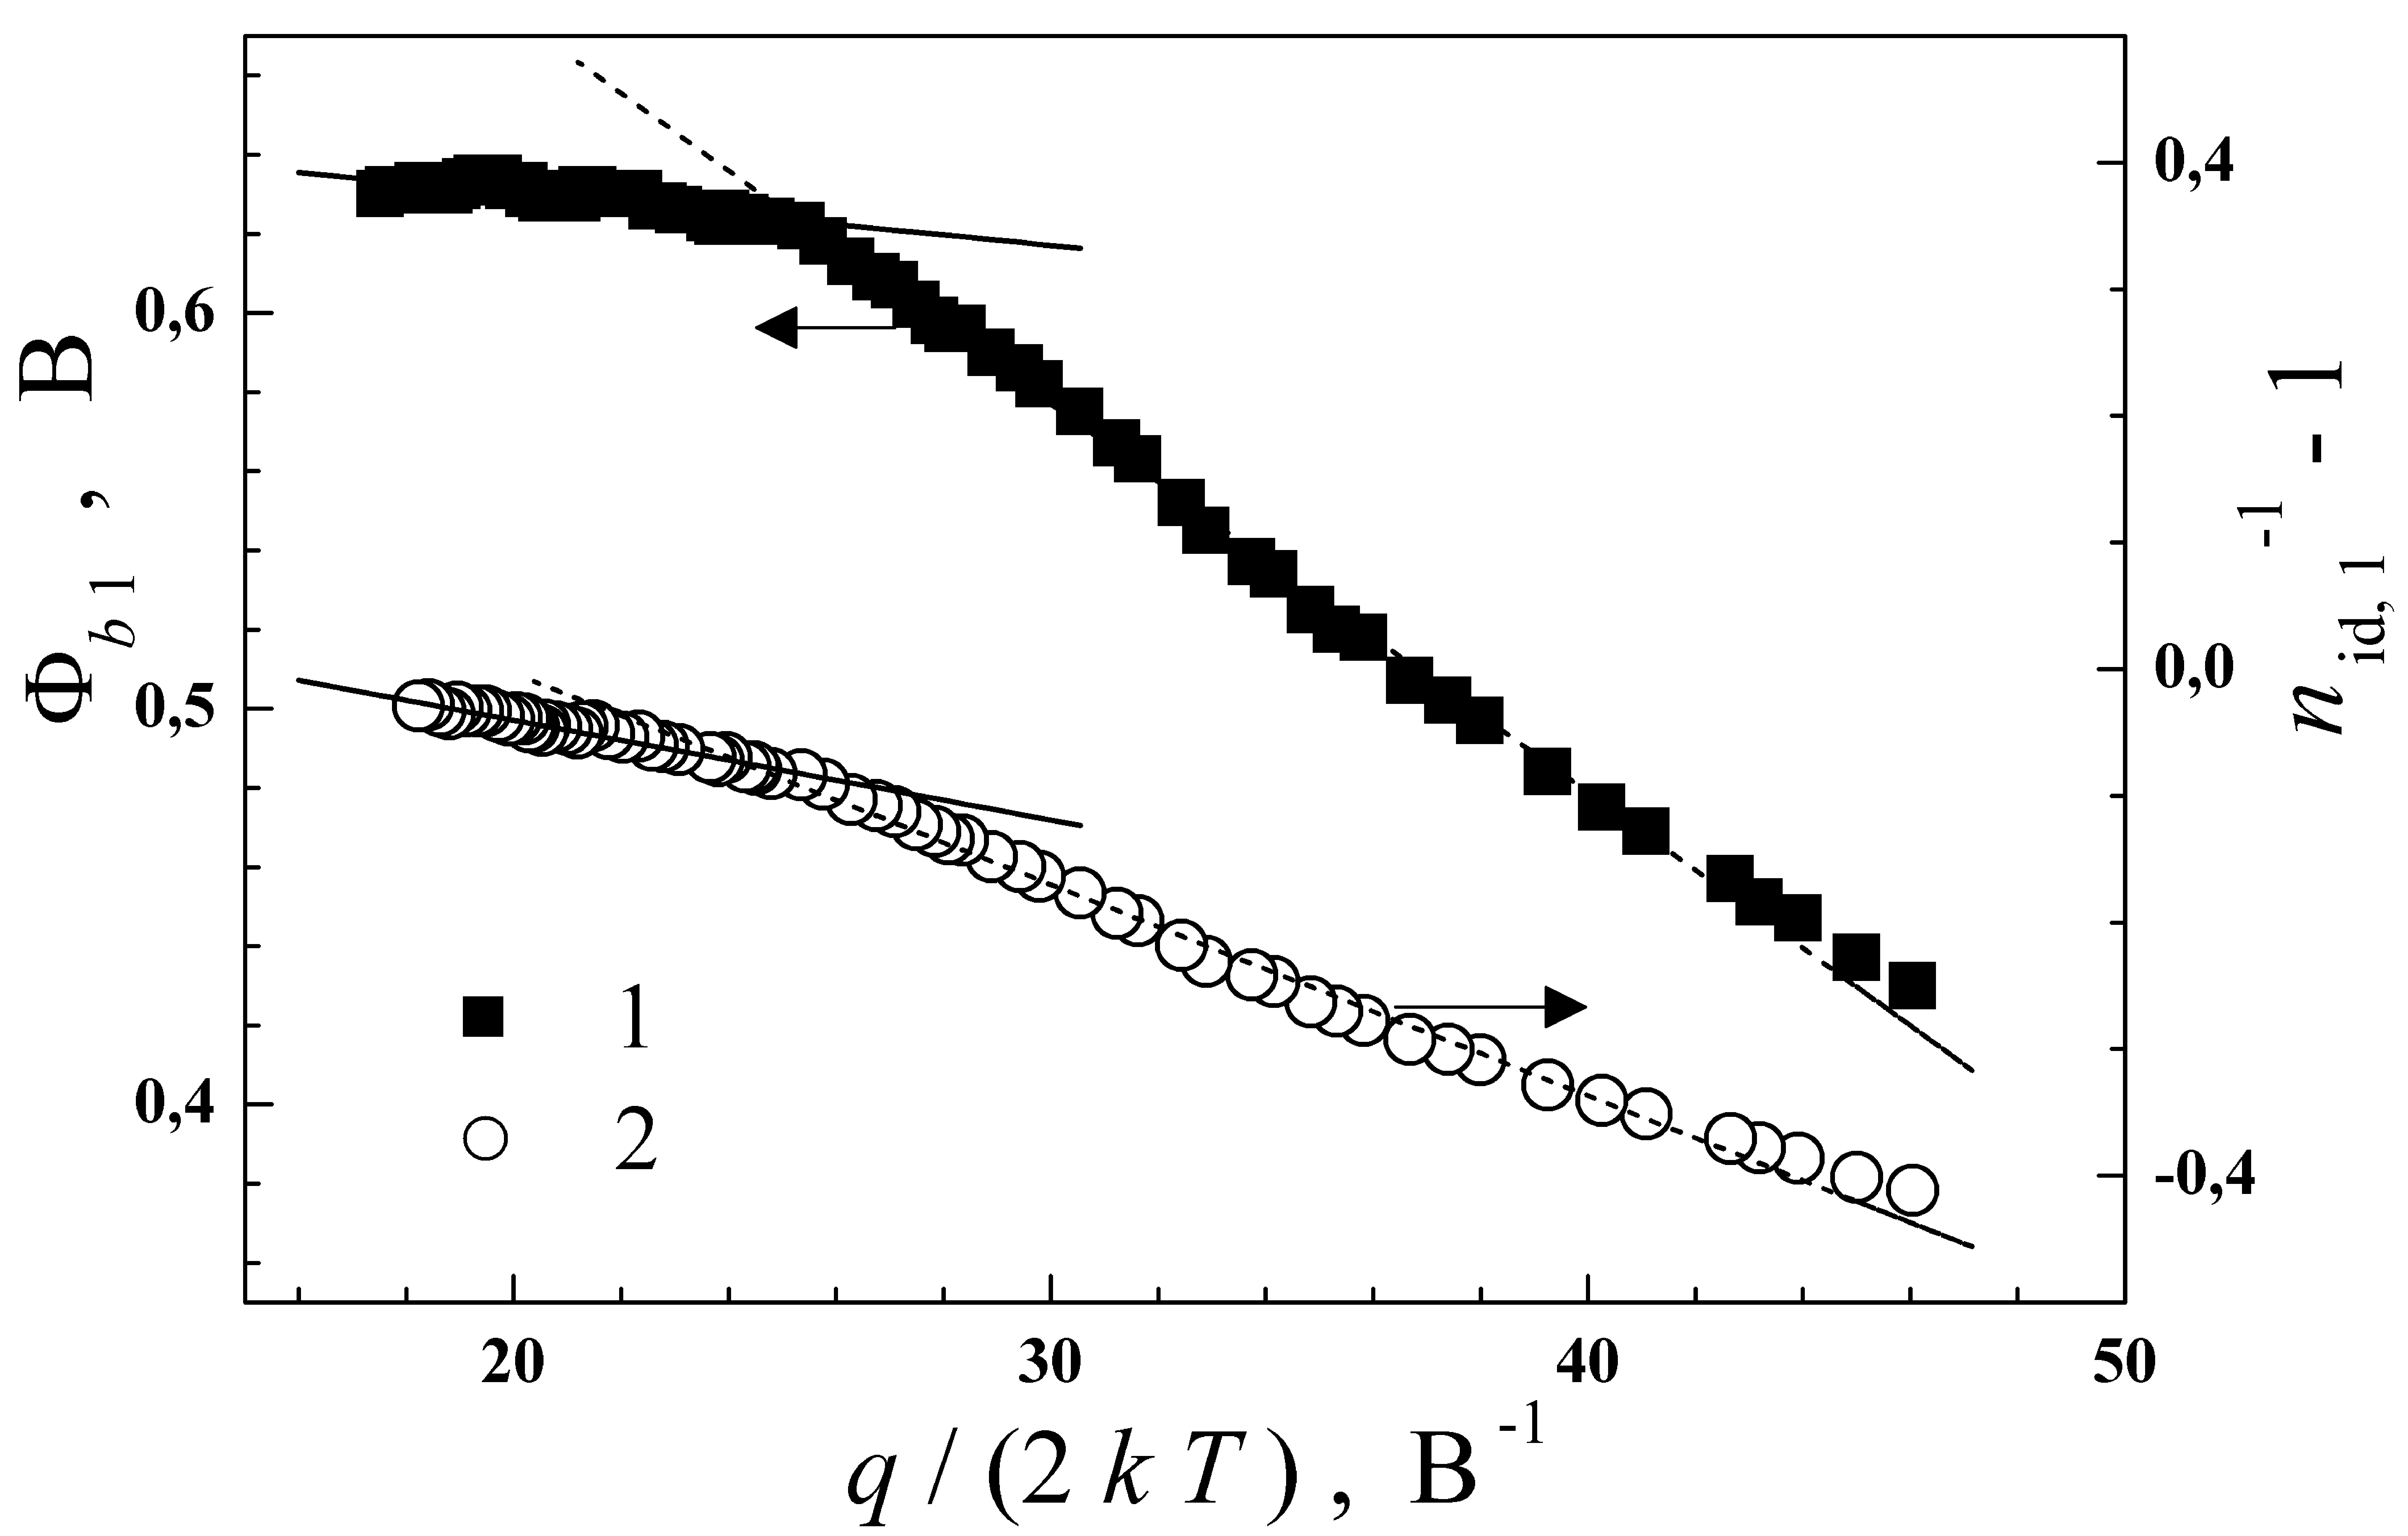
\includegraphics[width=0.7\textwidth]{figFbNT1_SDA}
\caption{\label{figFbNT1_SDA}
Залежності величин $\Phi_{b1}$ (крива 1) та $n_{\mathrm{id},1}^{-1}-1$ (крива 2) від оберненої температури.
Прямі --- лінійна апроксимація у діапазонах $T=(130\div220)$~К (суцільна) та $T=(230\div330)$~К (пунктир).
}%
\end{figure}

Використовуючи вираз (\ref{eqN_T0}) та значення $\Phi_{b}^0\simeq0.663$~В, $\sigma_{\Phi0}\simeq0.04$~В
була розраховане значення $T_{0,teor}\approx11$~К, яке очікується в рамках моделі контакту Шотки з локальними неоднорідностями
для температурного діапазону $(230\div330)$~К.
Ця величина досить близька до значення $T_{0,exp}\approx12$~К, отриманого експериментально (Рис.~\ref{figNT_SDA}) у цьому ж діапазоні.
Ще одним аргументом на користь того, що струм $I_1$ може бути описаний в рамках моделі ТЕ через неоднорідний контакт є якісний збіг
поведінки $n_{\mathrm{id},1}$ при низьких температурах (Рис.~\ref{figNT_SDA}) з очікуваною теоретично (\cite[Fig.11(b)]{Tung:PhysRev}).


У роботах  \cite{Tung:PhysRev,Sarpatwari,Schmitsdorf} показано, що для випадку
контакту з локальними неоднорідностями залежність між отриманими з аналізу ВАХ величинами $\Phi_b$ та $n_\mathrm{id}$ має бути лінійною,
причому $\Phi_{b}^0=\Phi_{b}+\Delta\Phi_b^\mathrm{IF}$ при $n=n_\mathrm{id}^\mathrm{IF}$
де $n_\mathrm{id}^\mathrm{IF}$ ---  величина фактору неідеальності з врахуванням впливу сил зображення,
$\Delta\Phi_b^\mathrm{IF}$ --- зниження бар'єру внаслідок дії сил зображення,
згідно з \cite{Sarpatwari}
\begin{equation}\label{eqN:IF}
n_\mathrm{id}^\mathrm{IF}\approx 1+\frac14\left[\frac{q^3N_d}{8\pi^2\varepsilon^2\varepsilon_0^2V^3_{bb}}\right]^{1/4},
\end{equation}
\begin{equation}\label{eqFb:IF}
\Delta\Phi_b^\mathrm{IF}\approx \left(\frac{q^3N_d\,V_{bb}}{8\pi^2\varepsilon^2\varepsilon_0^2}\right)^{1/4}.
\end{equation}
На залежності $\Phi_{b1}$ від $n_{\mathrm{id},1}$ (Рис.~\ref{figFbN_SDA}), як і в попередній випадках,
спостерігаються дві лінійні області зі зламом при $T\sim225$~К.
Шляхом екстраполяції отримано, що $\Phi_b^0$ дорівнює 0,646~В 0,64~В при низьких та високих температурах, відповідно.
Похибки визначення наведено в Таблиці~\ref{tabPar:SSDA}.
Зауважимо, що, згідно з \cite{Sarpatwari,Schmitsdorf},
при зниженні температури зростає роль проходження струму через патчі і, хоча лінійність між  $\Phi_b$ та $n_\mathrm{id}$ зберігається,
екстрапольоване значення ВБШ не буде дорівнювати висоті бар'єру в однорідній області.
На нашу думку, саме цим пояснюється відмінність величини $\Phi_b$, визначеної за залежністю
$\Phi_b=f(n_\mathrm{id})$ в низькотемпературному діапазоні, від інших,
отриманих для $T=(130\div220)$~К з використанням моделі неоднорідного бар'єру (див.~Таблицю~\ref{tabPar:SSDA}).

\begin{figure}
\center
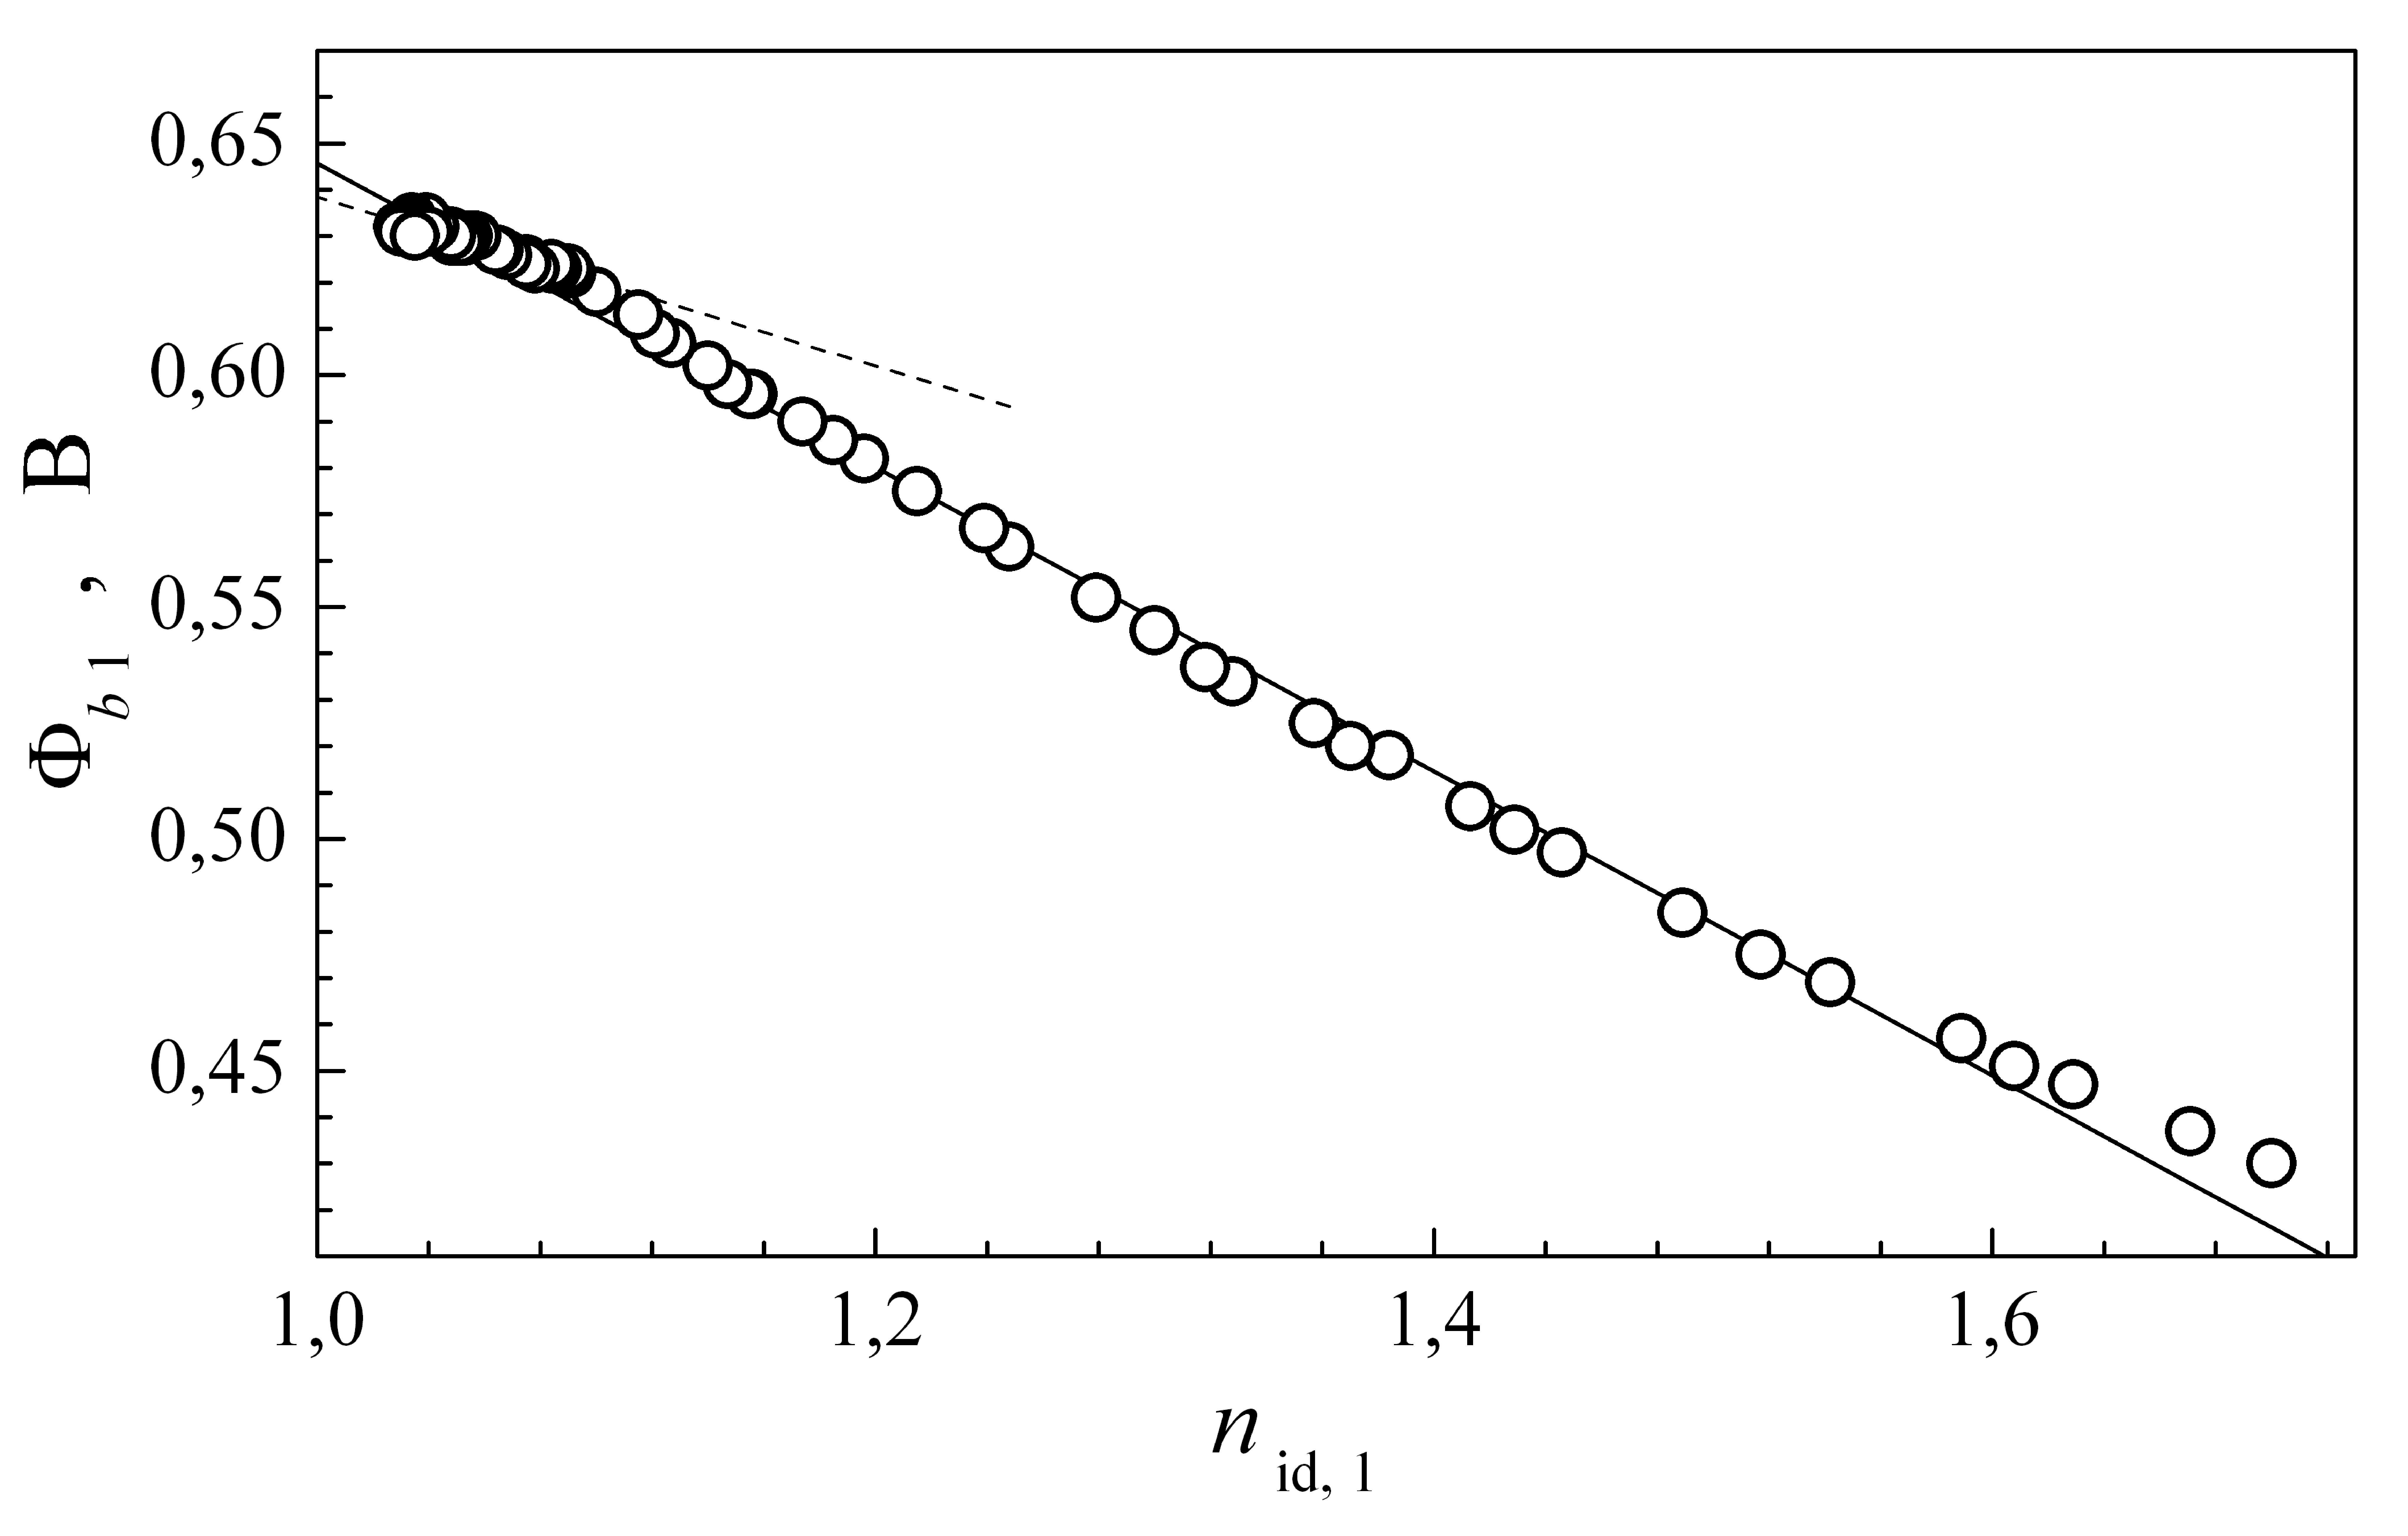
\includegraphics[width=0.7\textwidth]{figFbN_SDA}
\caption{\label{figFbN_SDA}
Залежність ВБШ від фактору неідеальності для високотемпературної компоненти струму $I_1$.
Прямі --- лінійна апроксимація у діапазонах $T=(130\div220)$~К (суцільна) та $T=(230\div330)$~К (пунктир).
}%
\end{figure}

У випадку неоднорідного бар'єру Шотки стала Річардсона може бути визначена за
допомогою модифікованої залежності Річардсона \cite{Tascioglu2010old,Yildirim2010}:
\begin{equation} \label{eqRich:Mod}
\ln\left(\frac{I_s}{T^2}\right)-\left(\frac{q^2\sigma_{\Phi0}^2}{2k^2T^2}\right)=\ln(AA^*)-\frac{q\Phi_b^0}{kT}.
\end{equation}

Відповідні графіки, побудовані з використанням отриманих значень $\sigma_{\Phi,0}$ показано на Рис.~\ref{figRichM_SDA}.
Лінійна апроксимація отриманих кривих у температурних діапазонах, відповідних тим, де були визначені стандартні відхилення
дозволили оцінити середнє значення ВБШ та сталу Річардсона.
Відповідні дані наведено в Таблиці~\ref{tabPar:SSDA}.
Зауважимо, що величини $A^*$, отримані в різних діапазонах температур в межах похибок збігаються
\begin{enumerate}[label=\asbuk*),leftmargin=0em,itemindent=1.5em]
\item між собою;
\item з літературними даними.
\end{enumerate}


\begin{figure}
\center
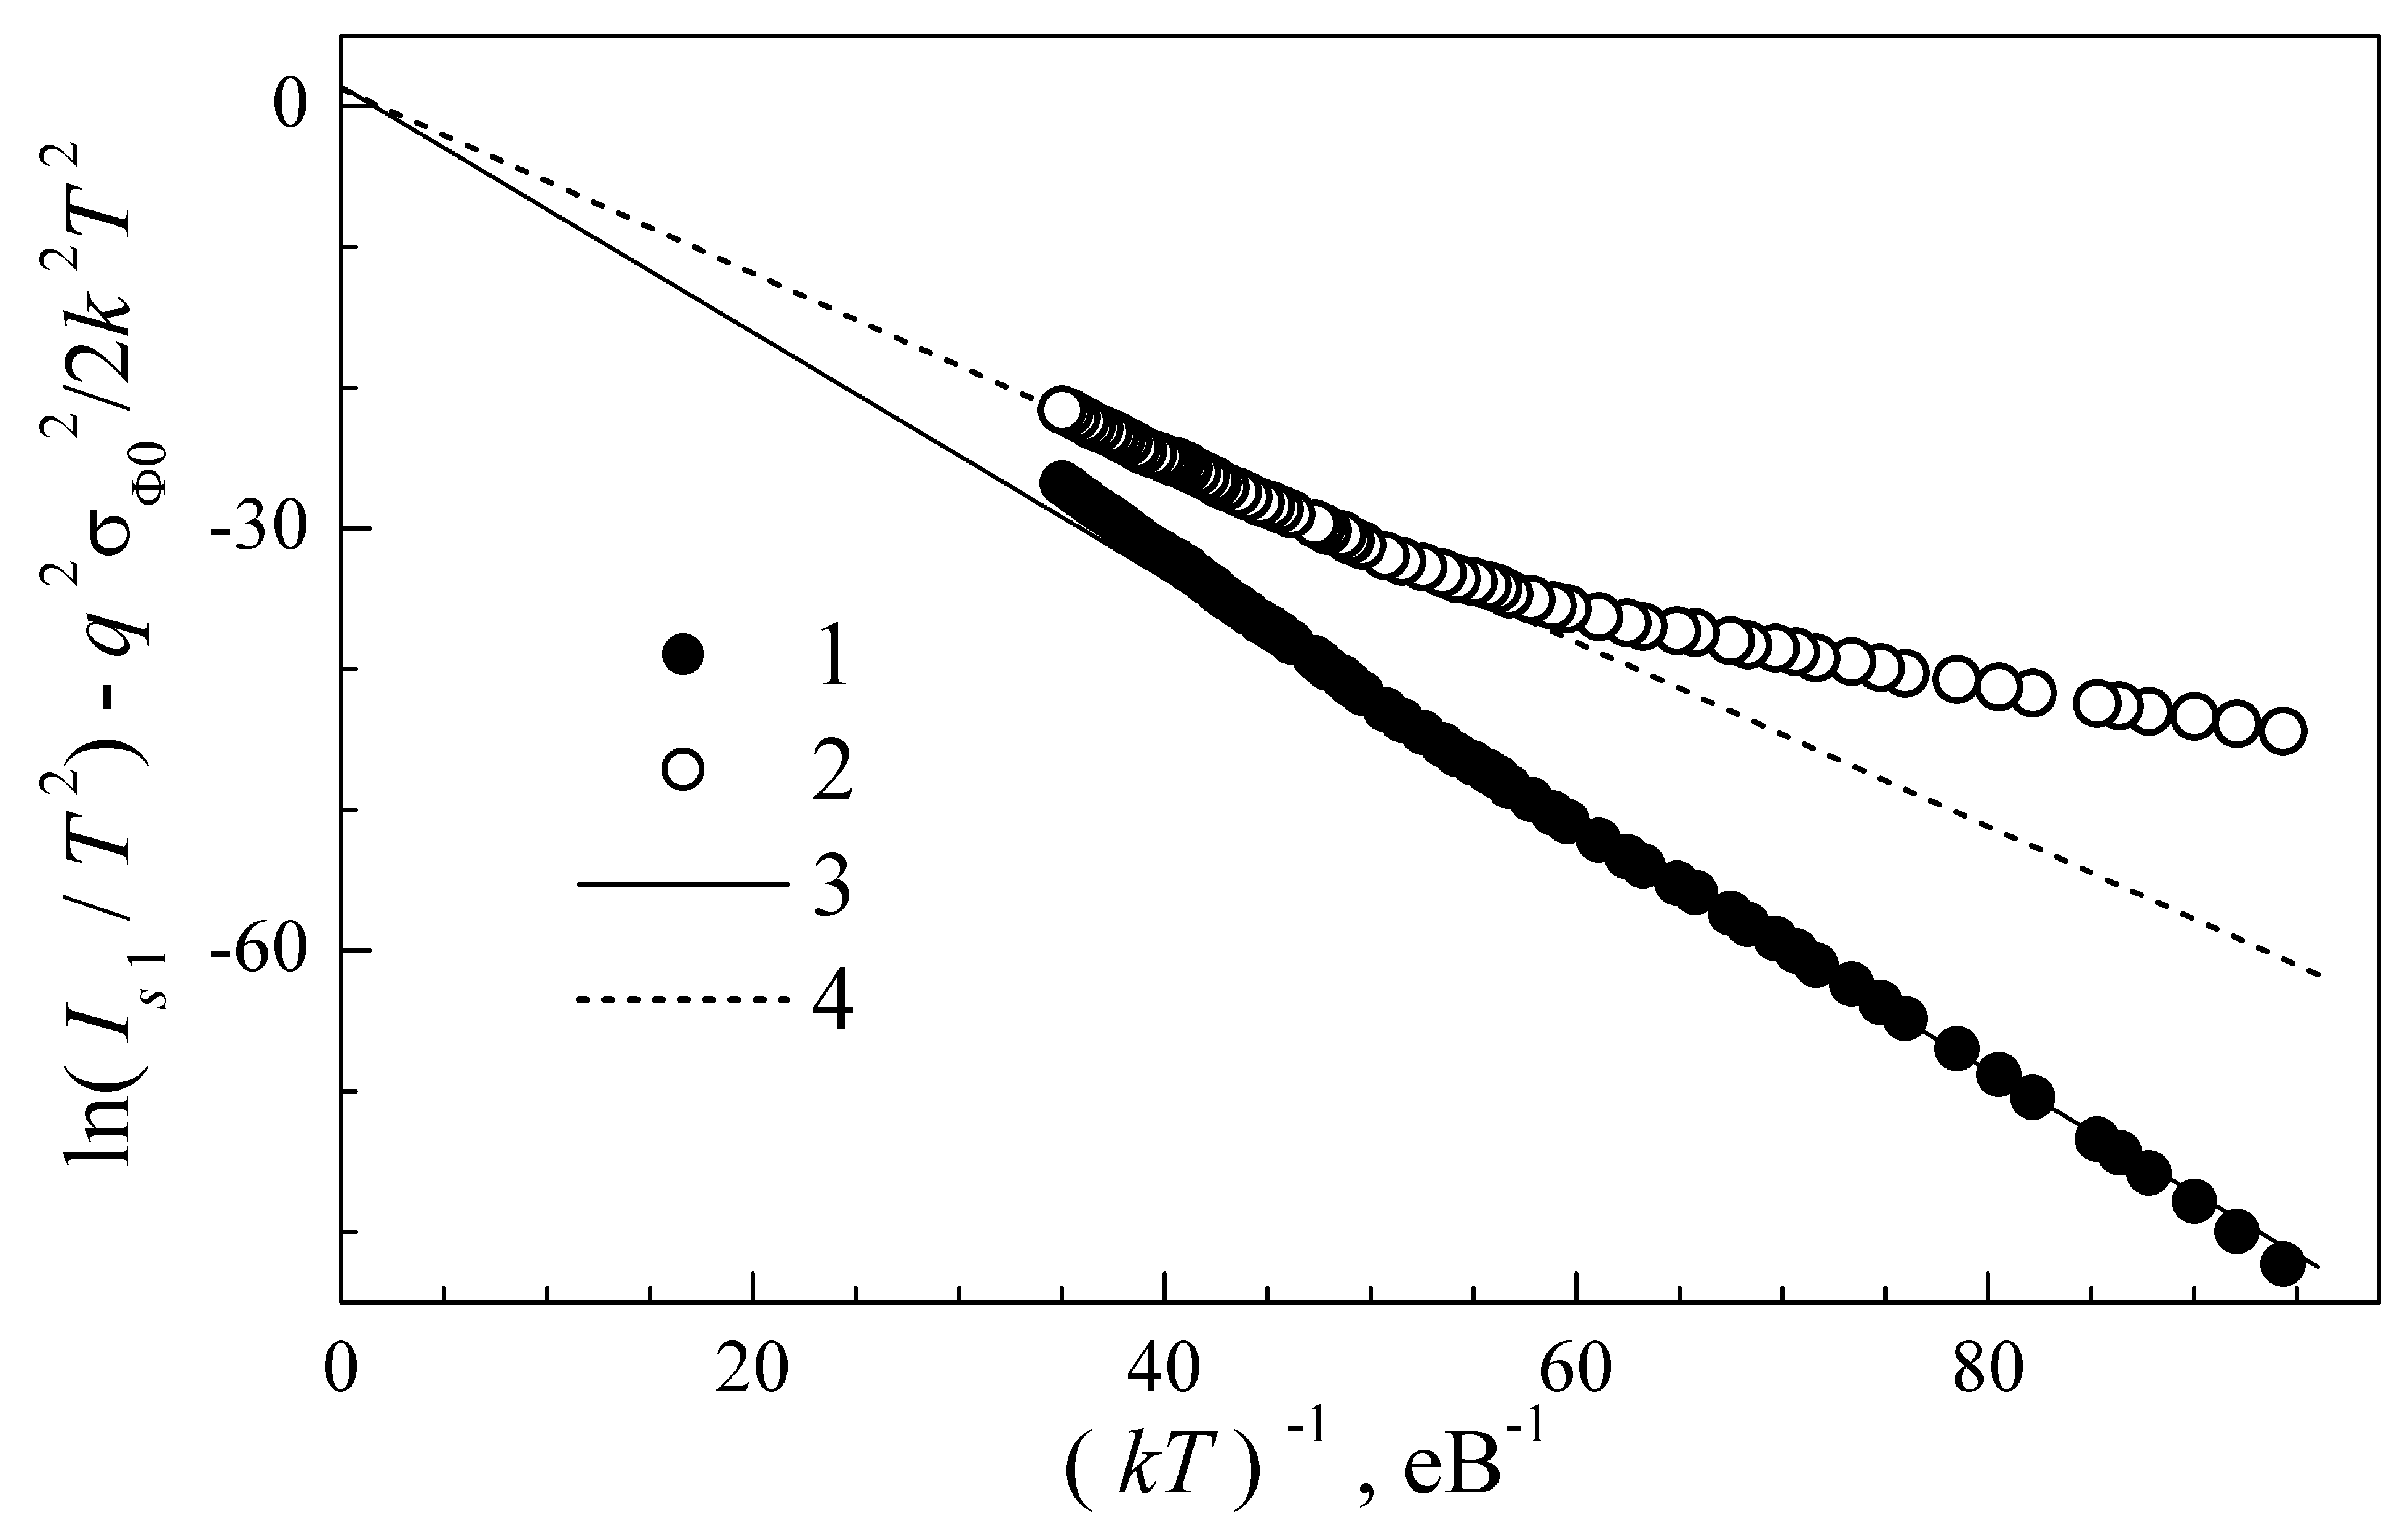
\includegraphics[width=0.9\textwidth]{figRichM_SDA}
\caption{\label{figRichM_SDA}
Модифіковані залежності Річардсона, розраховані за формулою (\ref{eqRich:Mod}) для $I_{s1}$.
$\sigma_{\Phi,0}$, В: 0,099 (крива 1) та 0,04 (2).
Прямі 3 та 4 --- лінійна апроксимація кривих 1 та 2 в діапазонах $T=(130\div220)$~К
та $T=(230\div330)$~К, відповідно.
}%
\end{figure}

В Таблиці~\ref{tabPar:SSDA} також наведено значення висоти бар'єру, визначене з ВФХ.
В цьому випадку  \cite{Rhoderick1988,Schroder2006}:
\begin{equation}\label{eqFbCV}
\Phi_{b,CV}=V_n+V_0+\frac{kT}{q},
\end{equation}
де
$V_0$ --- абсциса точки перетину з віссю напруг прямої, яка апроксимує залежність $1/C^2=f(V)$ (див. Рис.~\ref{figCV}).
Зазначимо, що визначена таким способом ВБШ має перевищувати величину, отриману за допомогою ВАХ
\cite{Rhoderick1988,GELCZUK2014,Mohan,Cetin2005,Soylu,Yildirim2010,Karatas:2006NIMA}.
Це пов'язано з тим, що $\Phi_{b,CV}$ визначається, насамперед, вигином зон і на неї не впливають, наприклад,
наявність сил зображення чи квантово--механічне тунелювання носіїв \cite{Rhoderick1988,GELCZUK2014,Mohan}.
Більше того, неоднорідність контакту також не відображається на величині $\Phi_{b,CV}$ на відміну від ВБШ,
яка визначається за допомогою ВАХ \cite{Sullivan,Tung:PhysRev,GELCZUK2014,Mohan}.
За своєю поведінкою зі зміною температури $\Phi_{b,CV}$ нагадує ВБШ, визначену за умов плоских зон, наближаючись
до неї і за величиною \cite{Cetin2005,Soylu,Yildirim2010,Mohan}.
В нашому випадку спостерігається очікуване співвідношення $\Phi_{b,CV}>\Phi_b^0$ для всіх значень, отриманих
в наближенні неоднорідного контакту.

Таким чином, наведені вище результати свідчать про те, що струм $I_1$ може бути описаний в рамках моделі ТЕ через неоднорідний бар'єр.
Єдине, що потребує більш детальної уваги --- відмінність між значеннями $\Phi_b^0$ та  $\sigma_{\Phi0}$ в різних температурних діапазонах,
яка напряму не передбачається в рамках теорії неоднорідного контакту.
Водночас подібна ситуація нерідко спостерігається експериментально, див., наприклад,
\cite{Tascioglu2010old,Yildirim2010,Mamor,Jiang:DGJap,JYOTHI2015,DURMUS2014,KHURE2015,OZAVCI2013,Tung:ApplPhysRev}.
Пов'язувалися подібні зміни  з домінуванням при низьких температурах інших, порівняно з ТЕ, механізмів перенесення заряду
(термопольова емісія, тунелювання чи рекомбінаційні процеси), фазовими перетвореннями в металі тощо.
Проте, на нашу думку, в даному випадку збіг  отриманих значень $A^*$ з літературними свідчить про застосовність саме теорії ТЕ.
Причиною зміни нахилів залежностей на Рис.~\ref{figFbNT1_SDA} та \ref{figRichM_SDA} може бути збільшення швидкості емісії електронів дефектами на границі МН.
Дійсно, звільнення рівнів окремих дефектів при $T\approx225$~K має стати причиною зменшення ВБШ, а також того,
що частина ділянок неоднорідності, в околі яких концентрація подібних дефектів підвищена, перестане бути зонами полегшеного проходження струму внаслідок ефективного захоплення дрейфуючих електронів пастками.
В результаті, у більш високотемпературному діапазоні $\sigma_{\Phi0}$ має зменшуватися, що і спостерігається на експерименті.
Інший варіант пояснення, який пропонується, зокрема, в роботі \cite{Tung:ApplPhysRev},
полягає в тому, що окрім патчів наявна додаткова неоднорідність інтерфейсу метал--напівпровідник.
Як правило, із ВАХ вдається визначити ВБШ для ділянок з меншим значенням $\Phi_b^0$ і лише при низькотемпературних вимірюваннях
нахил модифікованої залежності Річардсона дозволяє отримати інформацію про верхню границю розподілу висоти бар'єру.


Повернімось до струму $I_2$, який превалює при малих зміщеннях у низькотемпературній області.
В роботі~\cite{Tung:PhysRev} показано, що у випадку неоднорідного контакту такий додатковий, порівняно з $I_1$, струм
може з'являтися саме при низьких температурах внаслідок ефективного проходженню носіїв через патчі.
При цьому експериментальна залежність, показана на Рис.~\ref{figIV_SDA} дуже схожа на передбачену теоретично (див. Fig.6 в \cite{Tung:PhysRev}).
Крім того, у теорії очікується, що для відповідної ділянки ВАХ фактор неідеальності має значно перевищувати одиницю
і має спостерігатися суттєвий вплив послідовного опору.
Саме це і було виявлене в наших дослідженнях.
У випадку, коли струм через патчі визначається ТЕ, то, згідно з \cite{Sarpatwari, Tung:PhysRev},
\begin{equation}\label{eqIlowT}
I_s=f_pAA^*T^2\exp\left(-\frac{q\Phi_{b,p}}{kT}\right),
\end{equation}
де
$f_p$  --- множник, який враховує площу ділянок неоднорідності,
$\Phi_{b,p}$ --- ВБШ в області патчу.
Порівнюючи вирази (\ref{eqIlowT}) та (\ref{eqFb:TE}), можна
записати співвідношення між $\Phi_{b,p}$ та $\Phi_{b}$:
\begin{equation}\label{eqFbFbp}
\Phi_b=\Phi_{b,p}-\frac{kT}{q}\ln{f_p}\,.
\end{equation}
Як видно з рис.~\ref{figFbT_SDA}, величина $\Phi_{b2}$ дійсно є лінійною функцією температури.
Шляхом лінійної апроксимації експериментальних даних визначено, що $\Phi_{b,p}=(54\pm4)$~мВ,
$f_p=(8\pm1)\cdot10^{-13}$.
Таким чином, додатковий струм, який виникає при низьких температурах, також може бути пояснений з точки
зору моделі неоднорідного контакту Шотки.

\subsection{Перенесення заряду при зворотному зміщенні}

Приклади зворотних гілок ВАХ структур SSDA, виміряних при різних температурах, наведено на рис.~\ref{figIV_SDAr}.
Видно, що на представлених характеристиках не спостерігається насичення величини зворотного струму $I_R$.
Це свідчить про те,
що характеристики не можуть бути описані в рамках моделі ТЕ через бар'єр з постійною для певної температури висотою.
Зауважимо, що подібна поведінка (відсутність насичення зворотного струму) є типовою
практично для всіх реальних ДШ.
Це явище навіть отримало окрему назву --- <<м'які>> (<<soft>>) зворотні характеристики.

Зростання струму при підвищенні температури залежить від зміщення:
при збільшенні зворотної напруги $V_R$ температурна залежність $I_R$ послаблюється.
З метою визначення механізму перенесення заряду були побудовані залежності величини струму при певному значенні напруги від температури,
представлені на Рис.~\ref{figIT_SDAr}.
З рисунка видно, що
\begin{enumerate}[label=\asbuk*),leftmargin=0em,itemindent=1.5em]
\item при аналізі зворотних ВАХ також, як і для прямих гілок, доцільно розглядати два температурних піддіапазони $(130\div220)$~К та $(230\div330)$~К;
\item при зворотному зміщенні перенесення заряду забезпечується завдяки декільком механізмам.
\end{enumerate}



\begin{figure}
\center
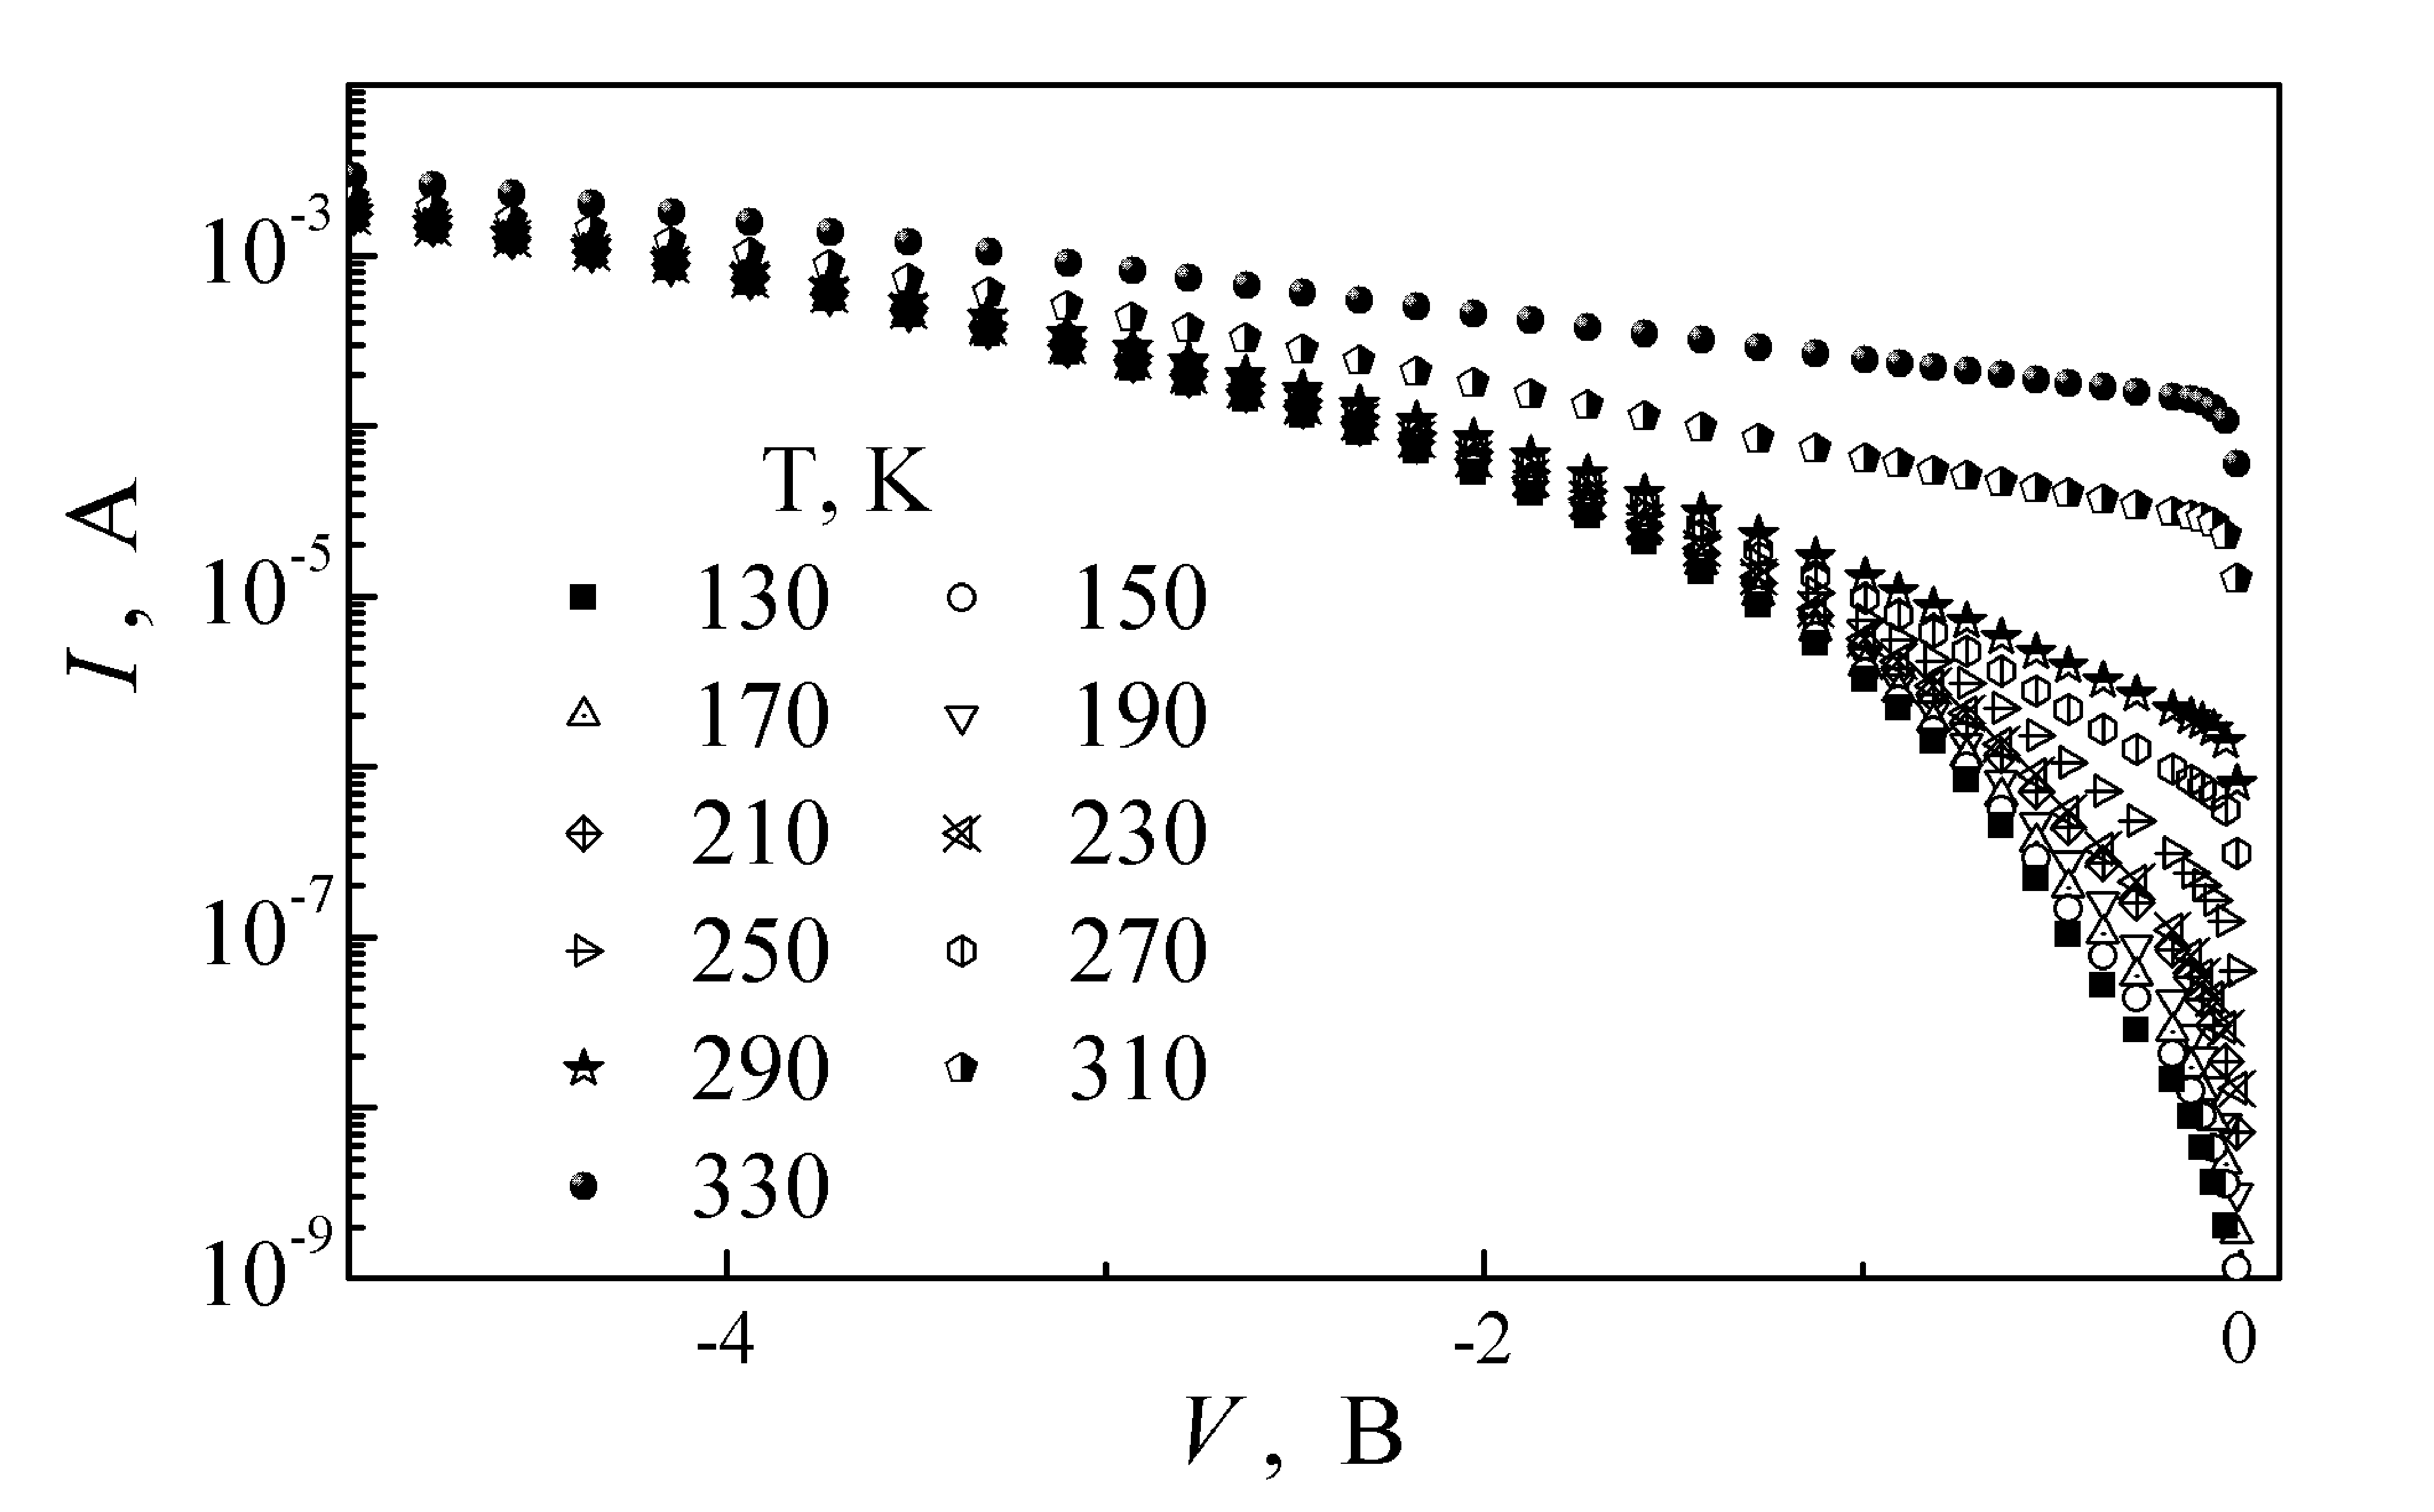
\includegraphics[width=0.8\textwidth]{figIV_SDAr}
\caption{\label{figIV_SDAr}
Зворотні характеристики структур SSDA при температурах 130~K (незаповнені точки)
та 330~K (напівзаповнені точки).
$D$, рад: 0 (квадрати), $10^6$ (трикутники), $10^7$ (кола).
}%
\end{figure}


\begin{figure}
\center
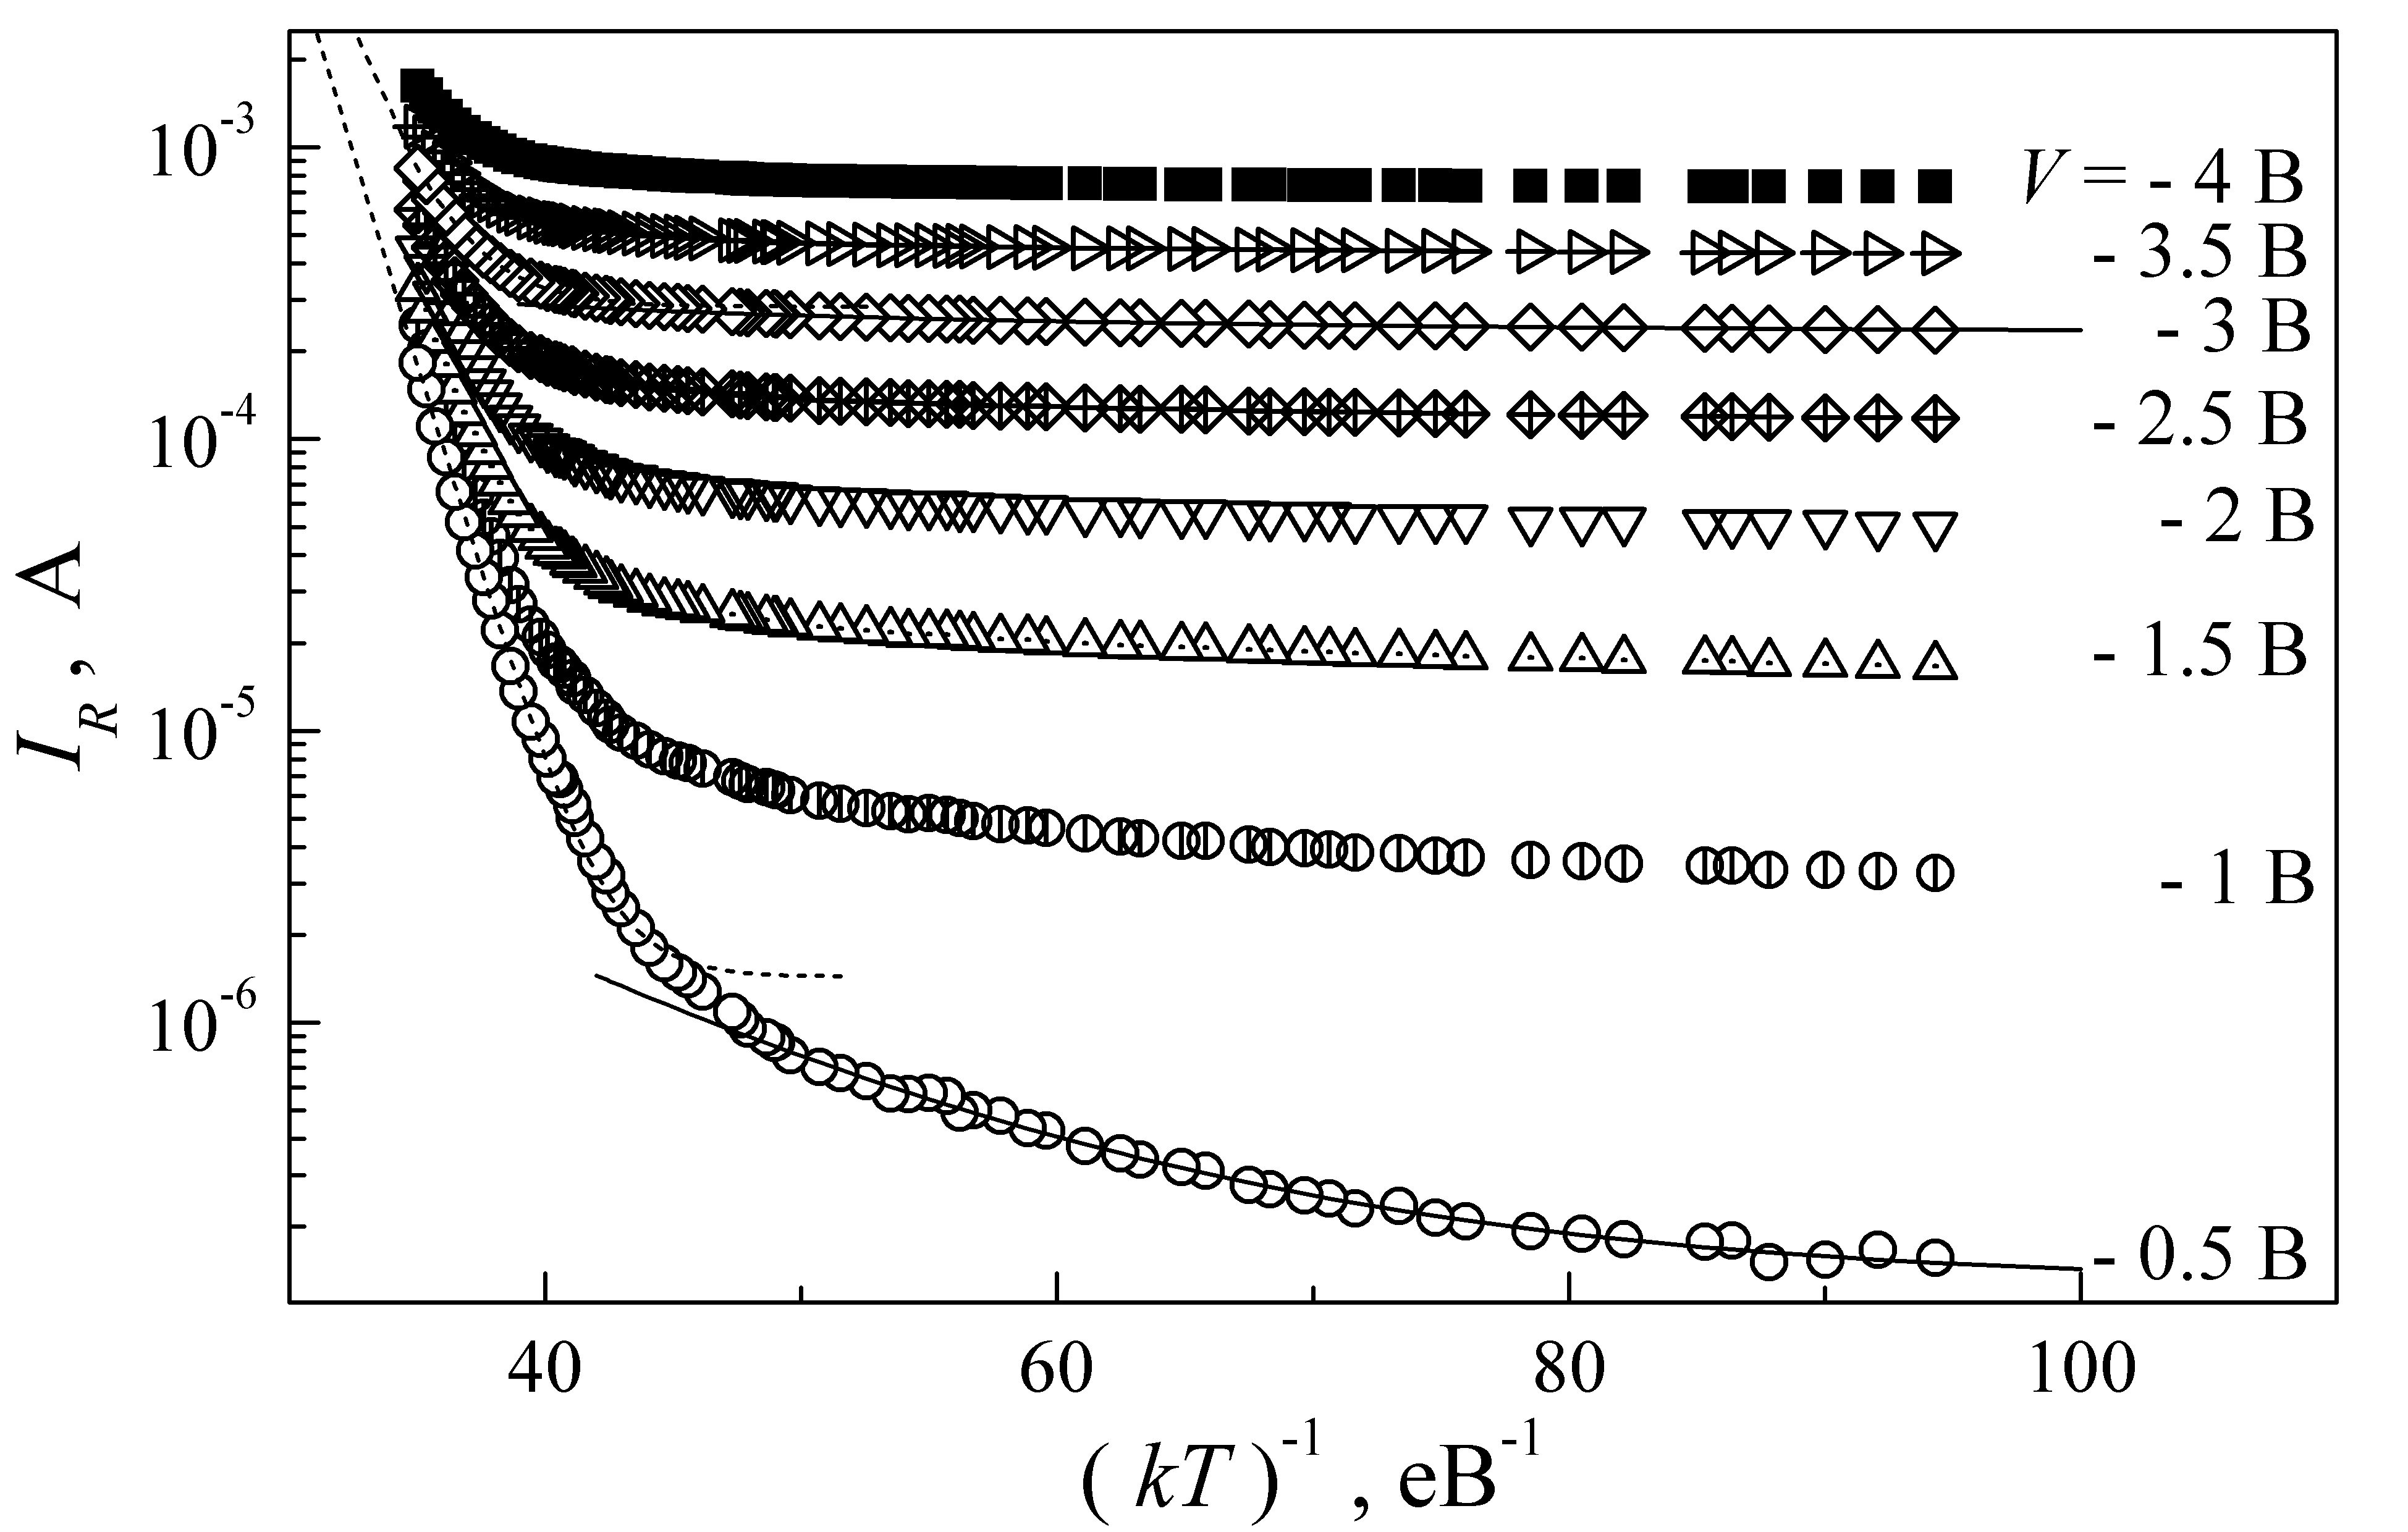
\includegraphics[width=0.7\textwidth]{figIT_SDAr}
\caption{\label{figIT_SDAr}
Температурна залежність зворотного струму структур SSDA при різних зміщеннях.
Точки --- експеримент, лінії --- апроксимація згідно з (\ref{eqIr})
(суцільні при $T=(130\div220)$~К, пунктирні при $T=(230\div330)$~К).
}%
\end{figure}

Проведений аналіз показав, що польова та температурна залежність зворотного струму можуть бути описані
за допомогою виразу
\begin{eqnarray}
\label{eqIr}
\nonumber I_R(T,V_R)&=&I_\mathrm{TE}(T,V_R)+I_\mathrm{FN}(V_R)=\\
&=&C_\mathrm{TE}(V_R)T^2\exp\left[-\frac{E_\mathrm{TE}(V_R)}{kT}\right]+I_\mathrm{FN}(V_R)\,,
\end{eqnarray}
де перший доданок $I_\mathrm{TE}$ описує ТЕ компоненту струму, яка залежить від температури та напруги,
а другий $I_\mathrm{FN}$ --- температурно-незалежну;
величини  $C_\mathrm{TE}$ та $E_\mathrm{TE}$ також не залежать від температури.

\label{nu_IR}
Для оцінки внеску кожної з компонент у загальний струм були використані величини
\begin{eqnarray*}
\nu_\mathrm{TE}&=&\frac{I_\mathrm{TE}}{I_R}=\frac{I_\mathrm{TE}}{I_\mathrm{TE}+I_\mathrm{FN}}\,,\\
\nu_\mathrm{FN}&=&\frac{I_\mathrm{FN}}{I_R}=\frac{I_\mathrm{FN}}{I_\mathrm{TE}+I_\mathrm{FN}}\,.
\end{eqnarray*}
Температурна та польова залежності $\nu_\mathrm{TE}$ та $\nu_\mathrm{FN}$ показані на Рис.~\ref{figeIr_SDA}.
Внесок ТЕ складової зростає при підвищенні температури та зменшенні зворотної напруги, проте характер
залежностей суттєво залежить від конкретних значень $T$ та $V_R$.


\begin{figure}
\center
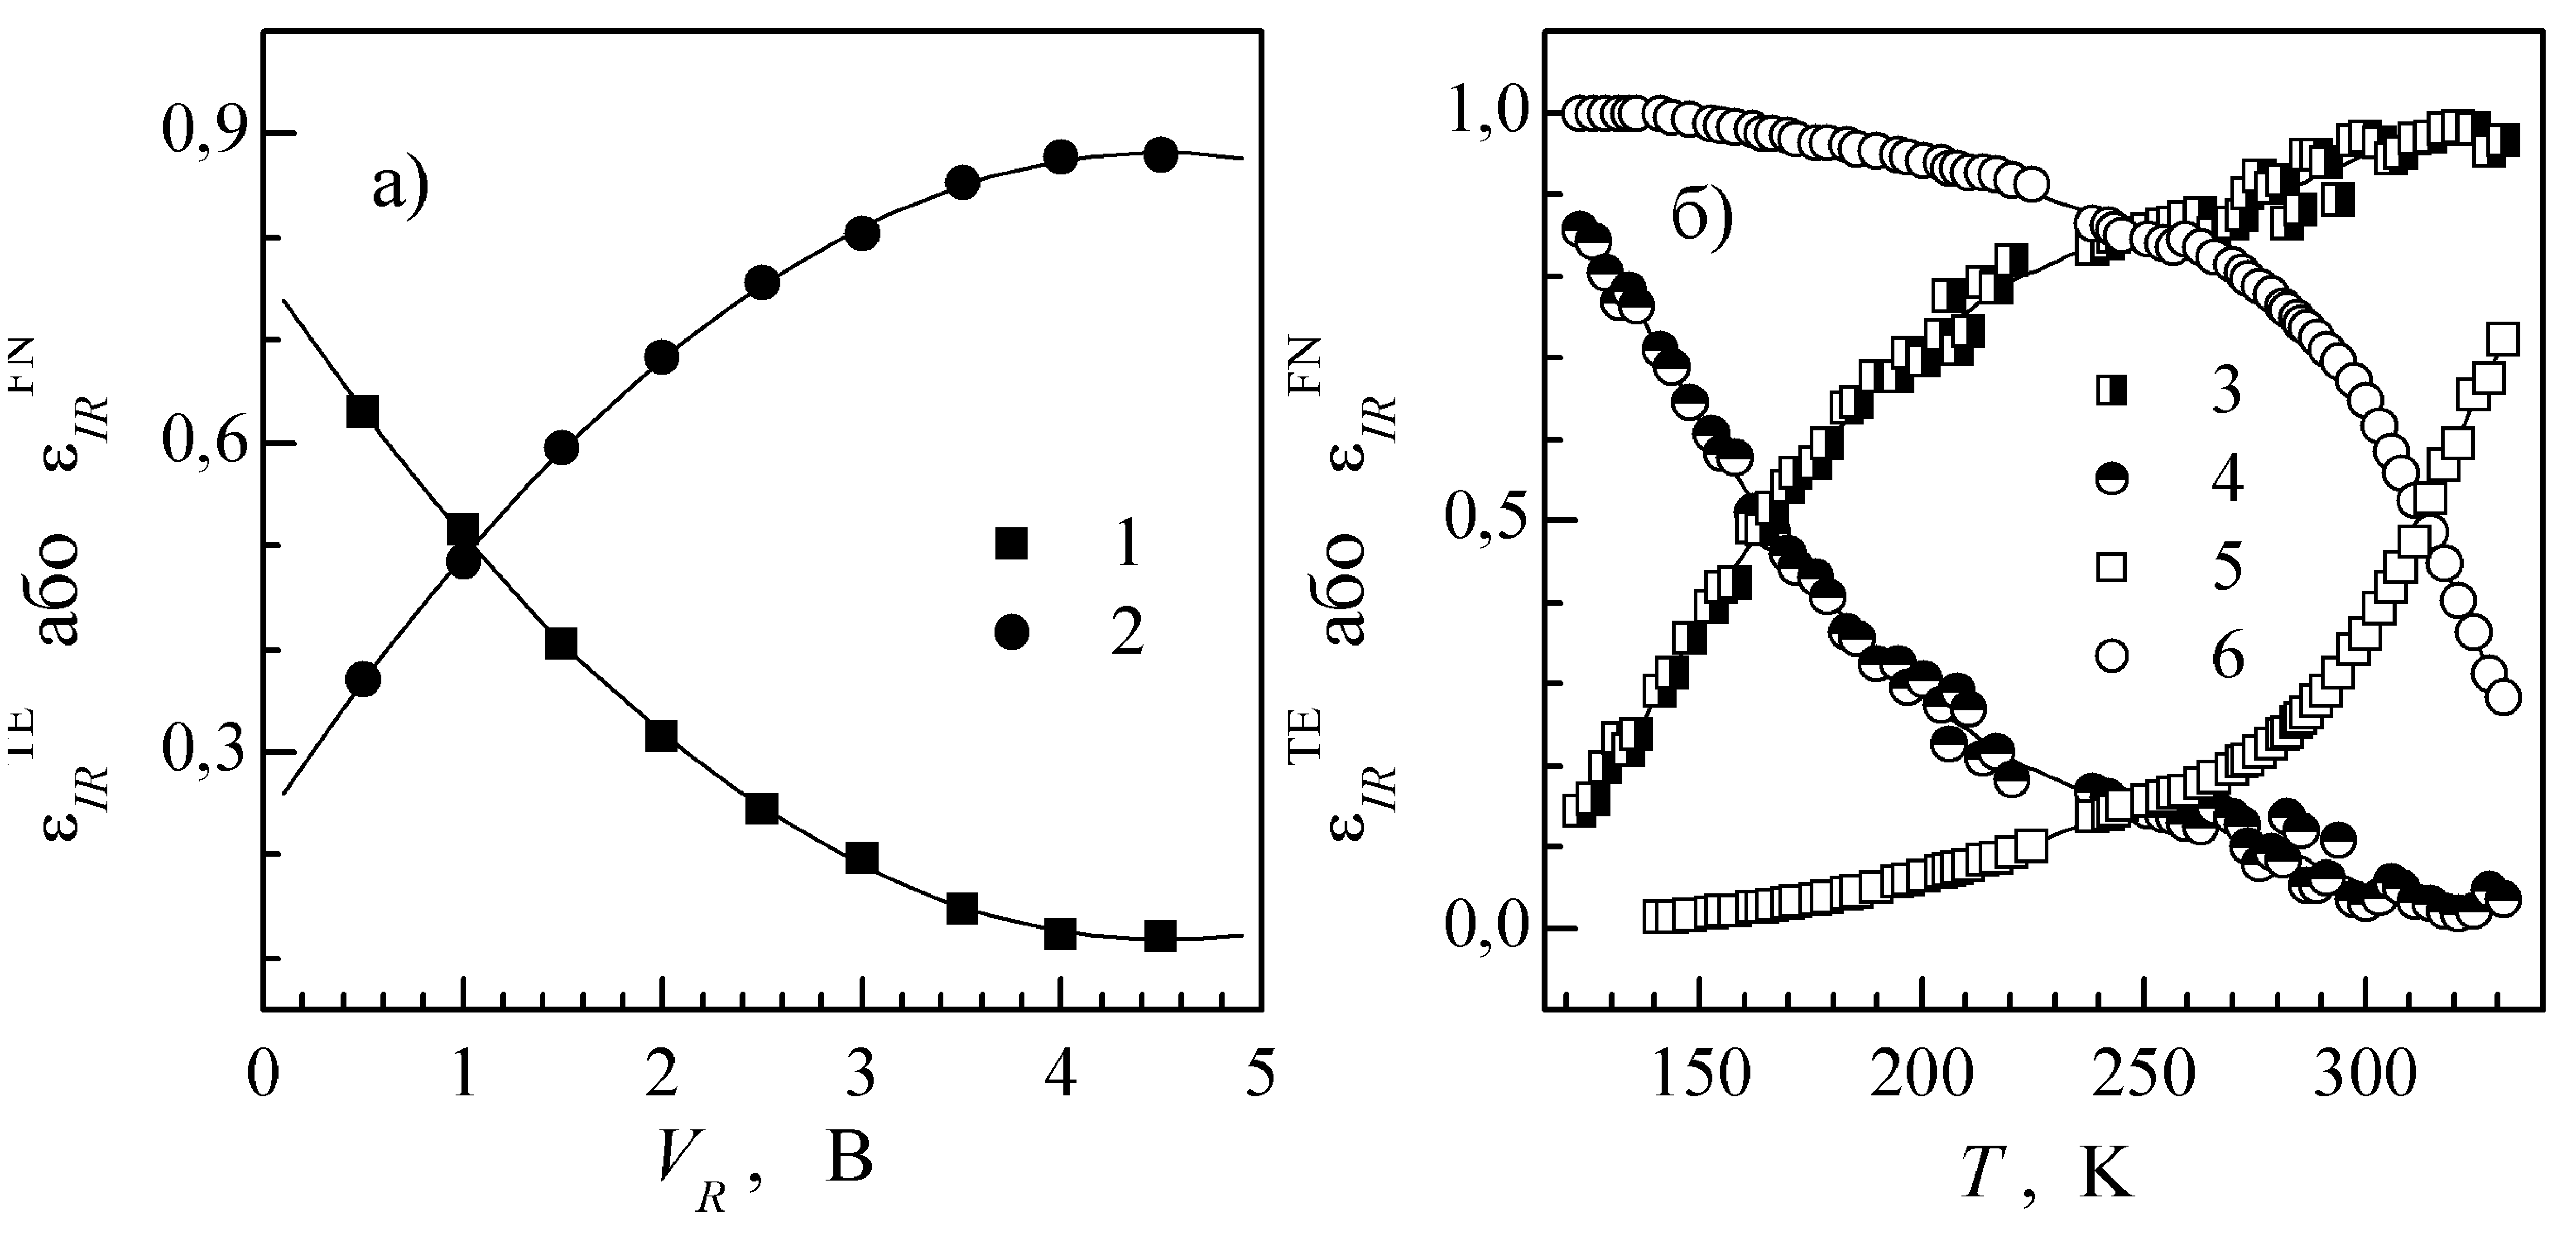
\includegraphics[width=0.8\textwidth]{figeIr_SDA}
\caption{\label{figeIr_SDA}
Залежність відносного внеску у зворотний струм
ТЕ (криві 1, 3 та 5) та температуро--незалежної (криві 2, 4 та 6)
компонент від зміщення при $T=300$~К (а) та
від температури (б) при $V_R=0,5$~В (3 та 4) і $V_R=3$~В (5 та 6).
}%
\end{figure}

Виявлена залежність характеристичної енергії $E_\mathrm{TE}$ від прикладеної напруги є свідченням зміни ВБШ.
Відомо \cite{Rhoderick1988,Tung:PhysRev,Andrews}, що зменшення висоти бар'єру при зворотному зміщенні може відбуватися під дією сил зображення
(при цьому  зміна ВБШ $\Delta\Phi_b\sim V_{bb}^{1/4}$),
електричного поля ($\Delta\Phi_b\sim V_{bb}^{1/2}$),
а також за рахунок впливу областей неоднорідності.
В останньому випадку за наявності неоднакових патчів $\Delta\Phi_b\sim V_{bb}^{2/3}$, а коефіцієнт пропорційності залежить від параметрів цих локальних ділянок \cite{Tung:PhysRev}.
Для досліджених структур $E_\mathrm{TE}$ набуває різних значень в кожному з температурних піддіапазонів,
проте при збільшенні зворотного зміщення в обох випадках зменшується, лінійно спадаючи з зростанням $V^{2/3}_R$ --- див. Рис.~\ref{figIrTE_SDA}.
Таким чином, аналіз зворотних ВАХ також підтверджує,
що струм через досліджувані структури може бути описаний в рамках теорії неоднорідного контакту з патчами,
вплив яких на зарядоперенесення змінюється поблизу температури 225~К.



\begin{figure}
\center
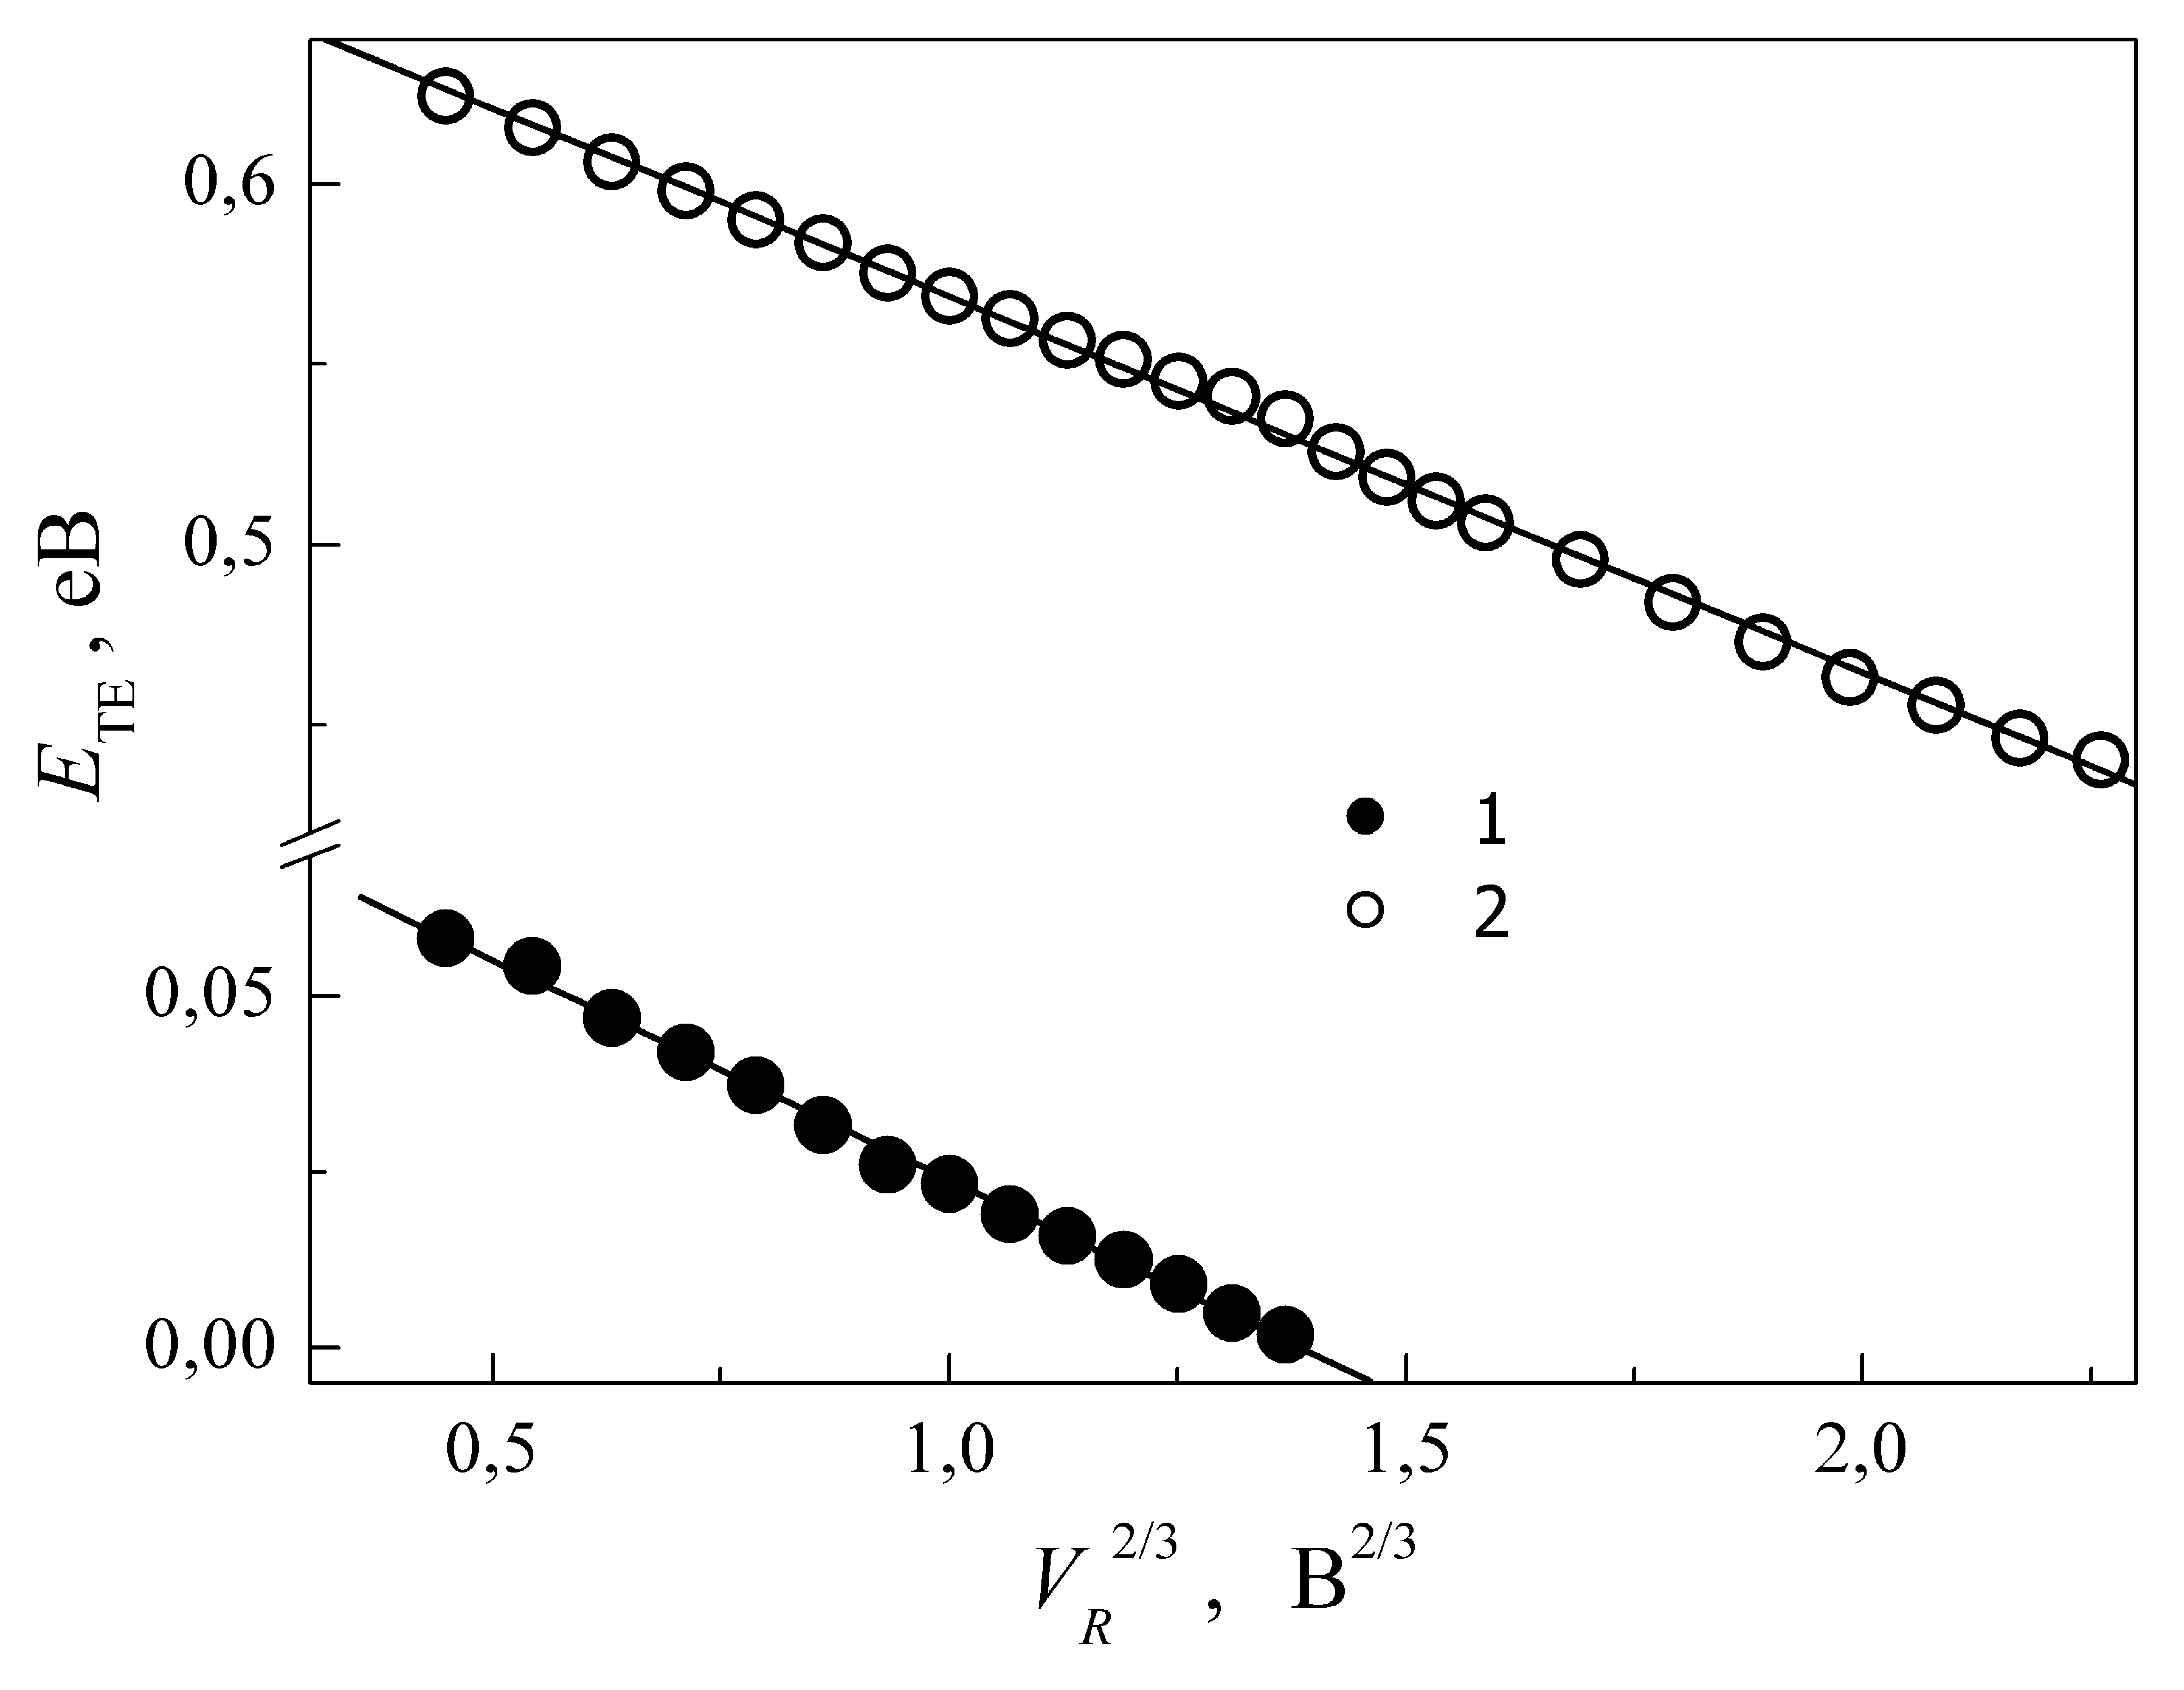
\includegraphics[width=0.65\textwidth]{figIrTE_SDA}
\caption{\label{figIrTE_SDA}
Польові залежності характеристичної енергії ТЕ складової зворотного струму
в діапазонах температур  $(130\div220)$~К (крива 1) та   $(230\div330)$~К (крива 2).
Точки --- експеримент, прямі --- лінійна апроксимація за методом найменших квадратів.
}%
\end{figure}

На Рис.~\ref{figIrFN_SDA} наведено польові залежності величини струму $I_\mathrm{FN}$ в координатах Фаулера--Нордгейма
$\ln(I_\mathrm{FN}/F_m^2)=f(1/F_M)$,
де
\begin{equation}\label{eqFm}
  F_m=\left(\frac{2qN_{d}V_{bb}}{\varepsilon_s\varepsilon_0}\right)^{1/2}
\end{equation}
напруженість електричного поля на границі розділу метал-напівпровідник \cite{Rhoderick1988};
при розрахунках $F_m$ використовувалися отримані при аналізі прямих ВАХ значення $\Phi^0_b$ та  $V_n$ при $T=250$~К.
Лінійність залежності свідчить про тунельний характер другої компоненти струму \cite{Evtuh},
що також підтверджується незалежністю величини $I_\mathrm{FN}$ від температури.


\begin{figure}
\center
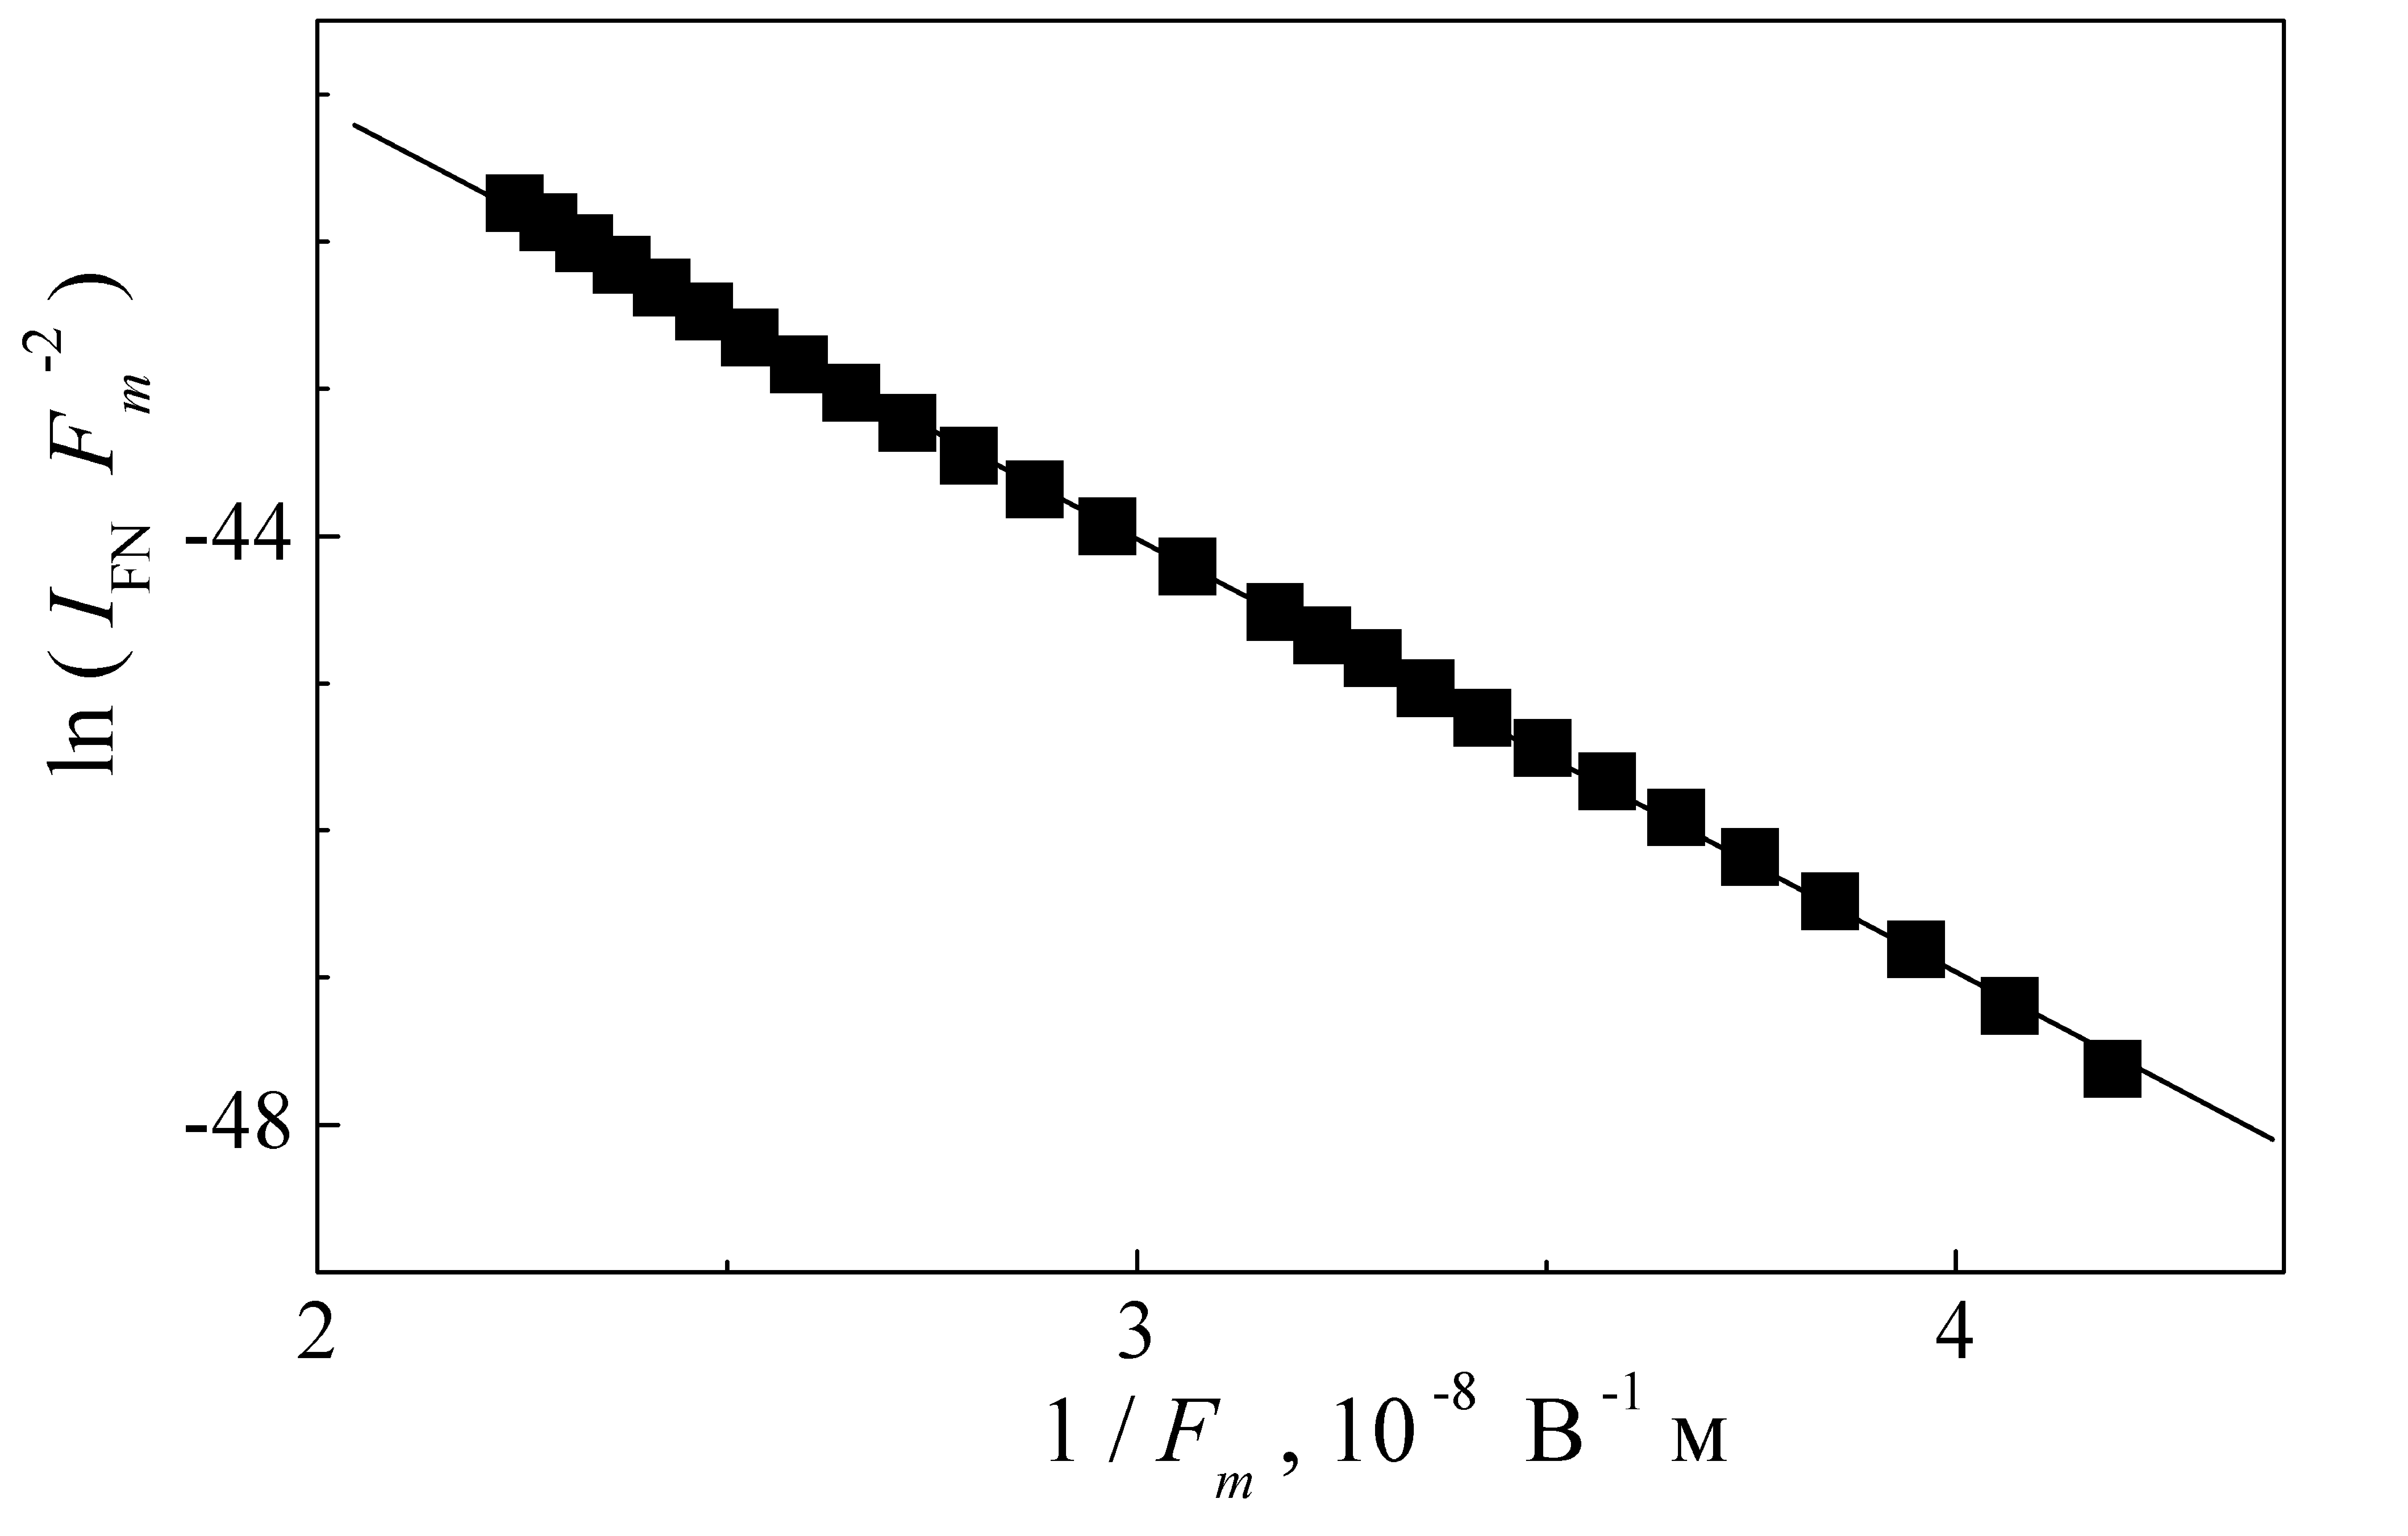
\includegraphics[width=0.65\textwidth]{figIrFN_SDA}
\caption{\label{figIrFN_SDA}
Залежність температуро--незалежної компоненти зворотного струму
в координатах Фаулера--Нордгейма.
Точки --- експеримент, пряма --- лінійна апроксимація за методом найменших квадратів.
}%
\end{figure}

Якщо тунелювання відбувається через трикутний бар'єр, то для опису струму може бути застосована
модифікована формула Фаулера--Нордгейма  \cite{Rhoderick1988,Novikov,Kurnosova}:
\begin{equation}\label{eqFowlNord}
    \ln\left(\frac{I_\mathrm{FN}}{F_m^2}\right)\propto -\frac{4 \sqrt{2m^*}(qE_{t,\mathrm{eff}})^{3/2}}{3\hbar q F_m}\,,
\end{equation}
де
$m*$ ---  ефективна маса електрону,
для Si $m* = 1,08\cdot9,11\cdot10^{-31}$~кг,
$E_{t,\mathrm{eff}}$ --– ефективна енергія тунелювання,
яка для випадку тунелюванням через центр у забороненій зоні залежить від глибини залягання рівня $\epsilon_t=E_c-E_t$ \cite{Kurnosova,Bulyarskii2001r}:
\begin{equation}\label{eqFN:Et}
    E_{t,\mathrm{eff}}=E_g\left\{\frac{3}{16}\left[\frac{\pi}{2}-
     \arcsin\left(1-\frac{2\epsilon_t}{E_g}\right)\right]-\frac{3}{8}\left(1-\frac{2\epsilon_t}{E_g}\right)
     \sqrt{\frac{\epsilon_t}{E_g}-\left(\frac{\epsilon_t}{E_g}\right)^2}\right\}^{2/3}
\end{equation}


Апроксимуючи отриману залежність (Рис.~\ref{figIrFN_SDA}) згідно з (\ref{eqFowlNord}) та використовуючи (\ref{eqFN:Et}),
знайдено, $E_c-E_t=(120\pm5)$~меВ.
Ця величина добре узгоджується з акцепторним рівнем міжвузольного атому вуглецю С$_i$: $E_c-(0,10\div0,12)$~еВ \cite{Vavilov1990r,Song1987}.
Таким чином, струм $I_\mathrm{FN}$ добре описується моделлю прямого тунелюванням через глибокий центр, яким, імовірно, є міжвузольний атом вуглецю.

\section{Вплив $\gamma$--опромінення на електрофізичні властивості структур Al$-n-n^+$--Si---Al\label{MSSi_Rad}}
Частина структур, використаних для досліджень, була опромінена гамма--квантами $^{60}$Co.
Як вже згадувалося, дослідженню впливу радіаційного опромінення на параметри ДШ приділяється значна увага.
Зокрема, достовірно виявлено \cite{Kumar1, Rao, Kumar2, Sharma, Ohyama}, що іонне та електронне опромінення ДШ,
створених на основі напівпровідників з електронною провідністю, викликає
монотонні (з підвищенням дози) зменшення висоти бар'єру та зростання фактору неідеальності і зворотного струму.
Ці ефекти виникають внаслідок утворення радіаційних дефектів, які спричинюють зміну концентрації вільних носіїв та
збільшення густини станів на інтерфейсній границі, що, в свою чергу, є причиною підсилення тунельного струму.
В той же час, у структурах з контактом Шотки, уражених внаслідок дії $\gamma$--квантів, незалежно від матеріалу чи типу провідності,
нерідко спостерігається збільшення ВБШ та зменшення фактору неідеальності \cite{Tataroglu,Tascioglu2010old,Tataroglu:2007NIMA}.
Для пояснення цього явища запропонований \cite{Tataroglu:2007NIMA} механізм, який передбачає
часткову компенсацію напівпровідника та інтенсифікацію інтерфейсних процесів тунелювання за участю рівнів дефектів (DAT, defect--assisted tunneling).
Проте, в літературі також зустрічаються повідомлення щодо зменшення ВБШ внаслідок $\gamma$--опромінення \cite{Tataroglu3}.
Більше того, якщо визначення ВБШ проводиться за допомогою ВАХ, то зі збільшенням поглинутої дози $\gamma$--квантів $^{60}$Co спостерігається
і немонотонні зміни висоти бар'єру \cite{Karatas:2006NIMA,Umana,Verma}.
До речі, дозова немонотонність зміни електричних параметрів спостерігається не лише при гамма--опроміненні ДШ,
але й для інших бар'єрних структур \cite{Kinoshita} та/або типів радіаційного впливу \cite{Vorobets, Pattabi, Kovalyuk}.
Нарешті, варто зауважити, що виявлені немонотонності впливу опромінення на структури МН також бувають різного типу:
наприклад, в роботах \cite{Karatas:2006NIMA, Vorobets, Pattabi} виявлено, що ВБШ збільшується
при малих дозах і зростає при великих, тоді як автори робіт \cite{Umana,Verma} описують протилежну тенденцію.
Причини подібних розходжень до цього часу не знайшли належного пояснення.

В нашому випадку доза $\gamma$--опромінення складала $10^6$ або $10^7$~рад, для позначення відповідних зразків, як і в розділі~\ref{Ch_SSC}, використовуються префікси <<g6>> та <<g7>>, відповідно.
При виборі дози були використані результати роботи \cite{Karatas:2006NIMA}, де показано,
що ВБШ кремнієвих структур зростає, якщо загальна поглинута доза $\gamma$--квантів $^{60}$Co $\approx10$~кГр, тоді як при подальшому збільшенні
$D$ до $100$~кГр висота бар'єру зменшується.
Водночас, використані дози не викликають значних порушень кристалічної ґратки,
про що, зокрема, свідчить, відсутність впливу $\gamma$--опромінення на концентрацію вільних носіїв заряду --- див. Рис.~\ref{figCVrad}

\begin{figure}
\center
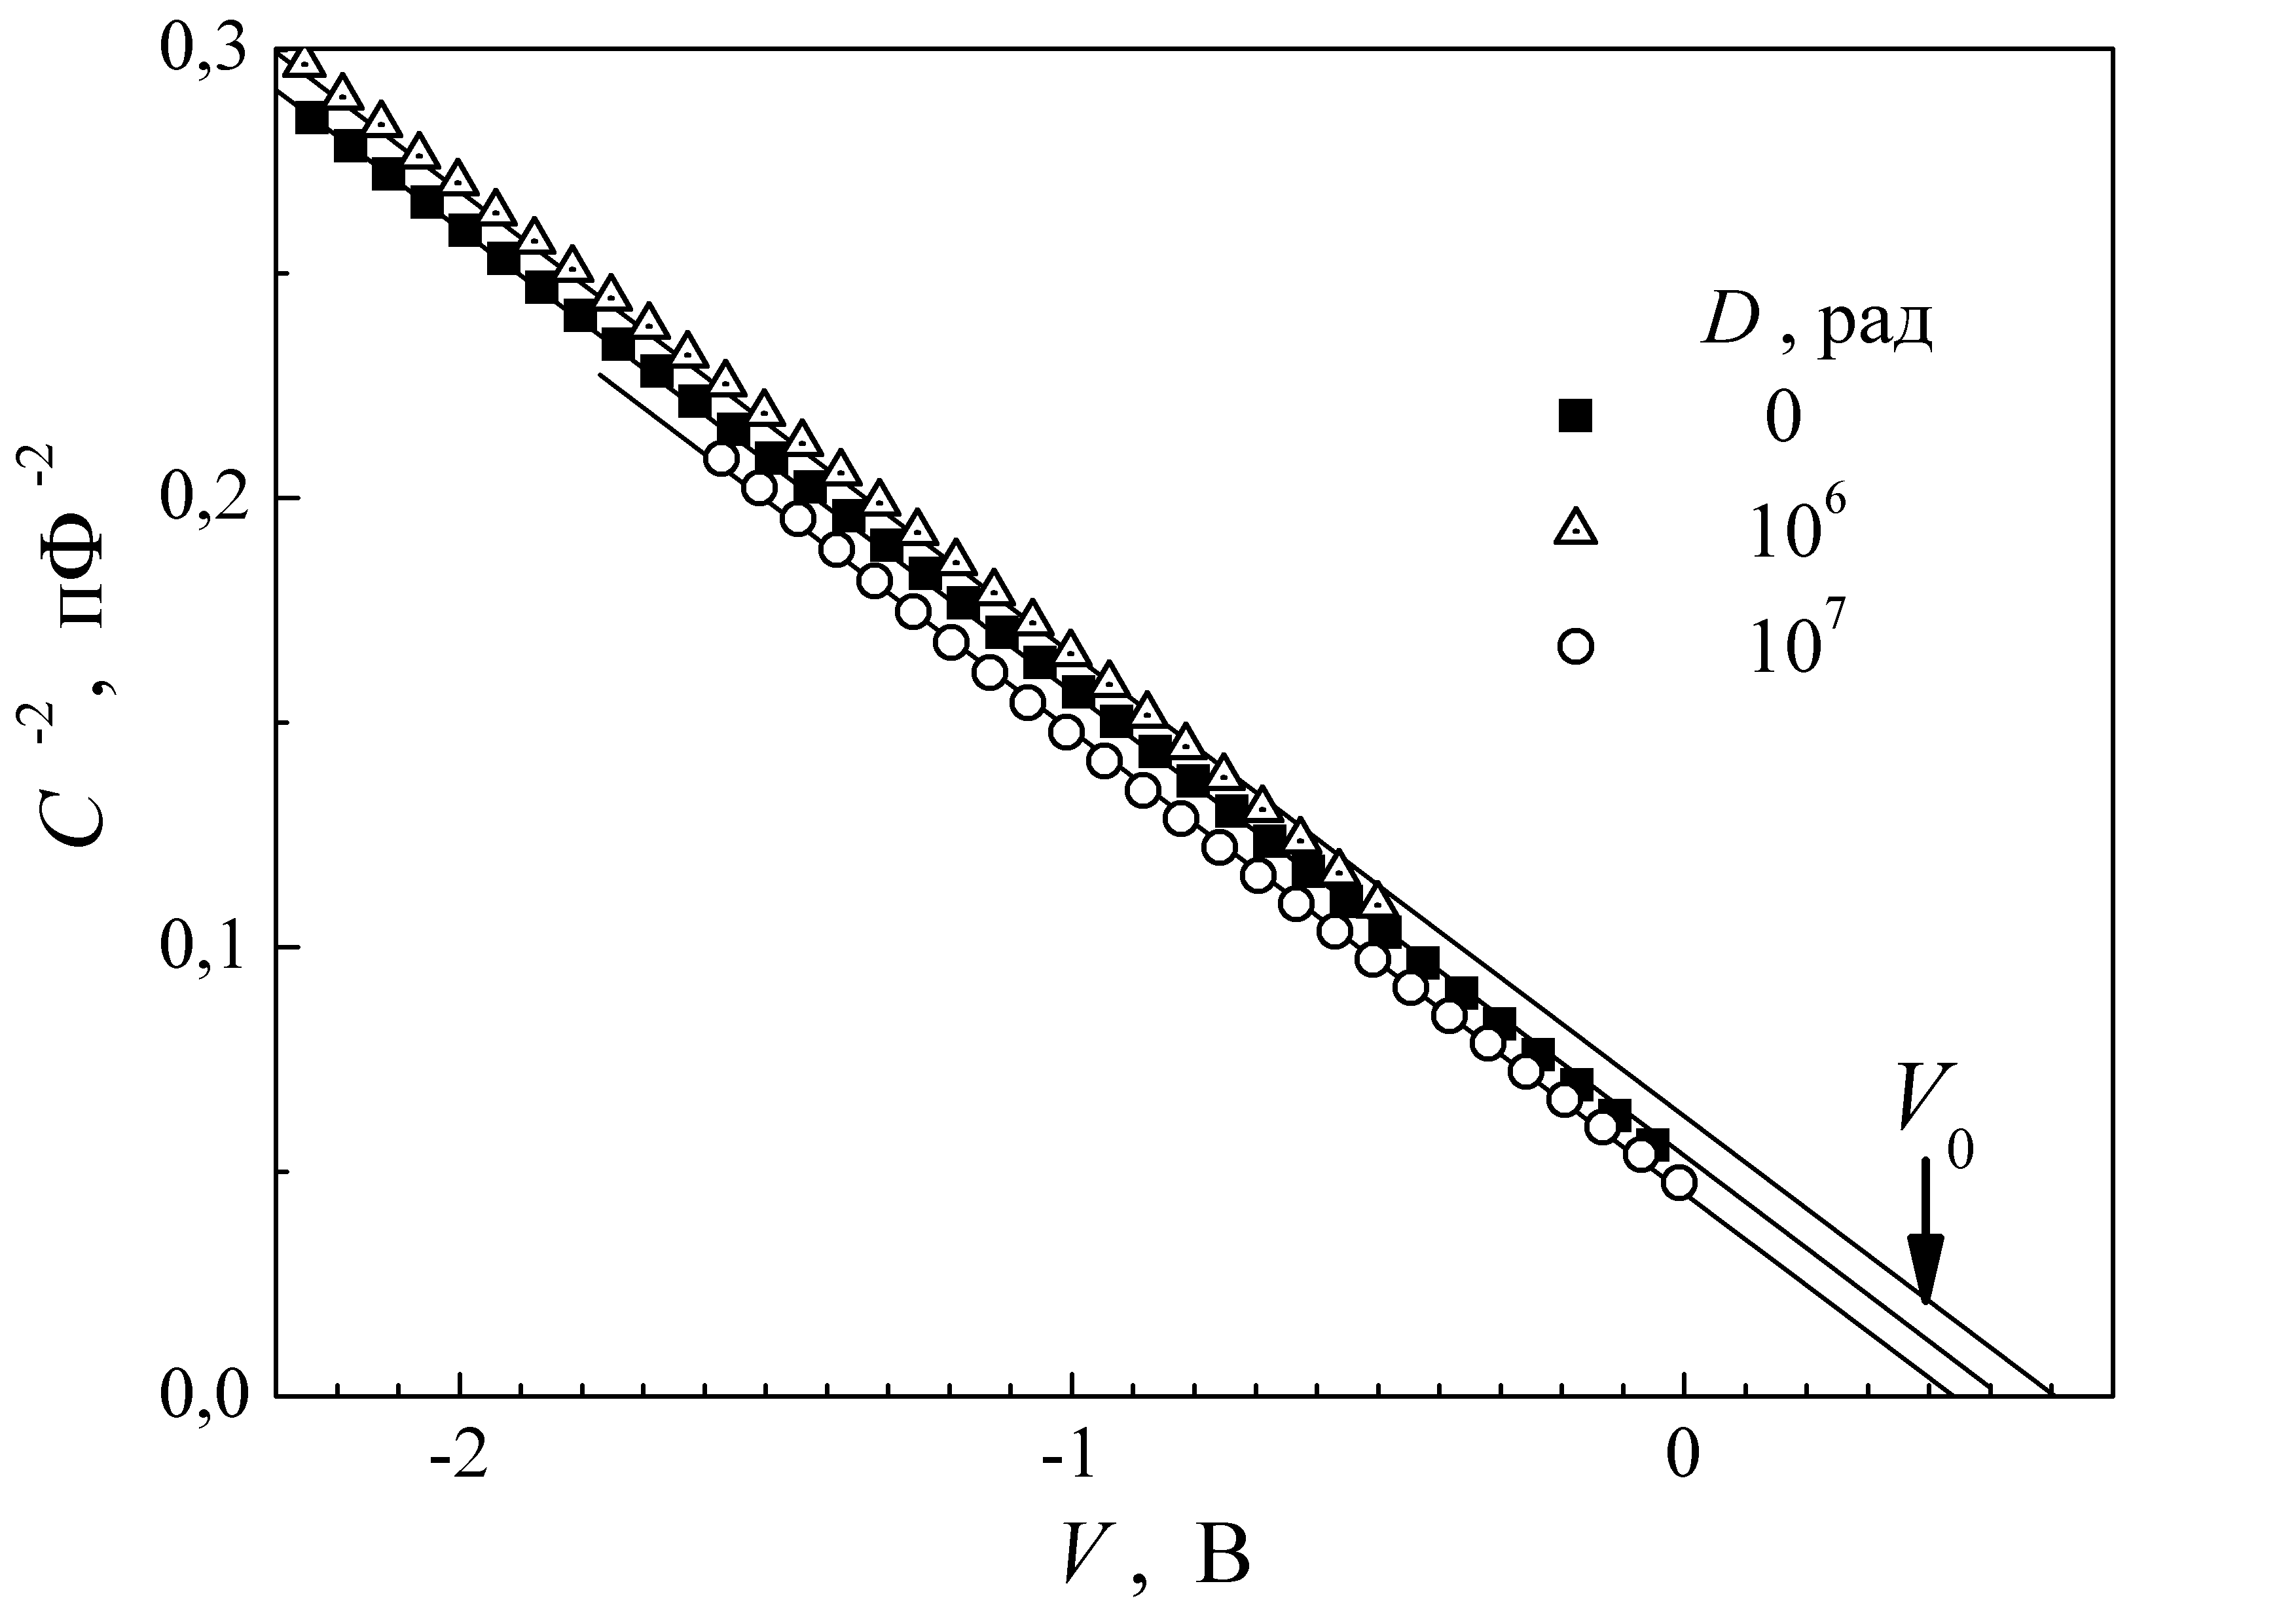
\includegraphics[width=0.7\textwidth]{figCVrad}
\caption{\label{figCVrad}
Вольт--фарадні характеристики структур Al$-n-n^+$--Si---Al з різним ступенем опромінення.
Точки --- експеримент, пряма --- лінійна апроксимація.
}%
\end{figure}

%виміри показали, що $N_d$ дорівнює $1.10\cdot10^{23}$ та $1.19\cdot10^{23}$ м$^{-3}$ для g6SSDA та g7SSDA, відповідно.

Нижче, поряд з отриманими результатами для опромінених зразків, нерідко наведено також дані і для неопромінених,
які детально розглянуті у попередньому підрозділі.
Це зроблено з метою зручності порівнянь змін, викликаних опроміненням.


\subsection{Прямий струм у $\gamma$--опромінених кремнієвих діодах Шотки}

На Рис.~\ref{figIVrad_SDA} представлено результати вимірювань прямих гілок ВАХ структур Al$-n-n^+$--Si---Al, опромінених
$\gamma$--квантами $^{60}$Co з різною величиною поглинутої дози.
Як і для неопромінених (див. Рис.~\ref{figIV_SDA}) видно, що струм складається з двох складових.
Одна переважає при великих зміщеннях та високих температурах; надалі для скорочення називатимемо її
<<високотемпературною компонентою струму>> (ВТКС), хоча, можливо, ця назва і не повністю віддзеркалює її поведінку.
Внесок другої стає помітним при низьких температурах ($T<250$~К) і лише при малих напругах ($V<0,2$~В);
для її позначення будемо використовувати словосполучення <<низькотемпературна компонента струму>> (НТКС).


\begin{figure}
\center
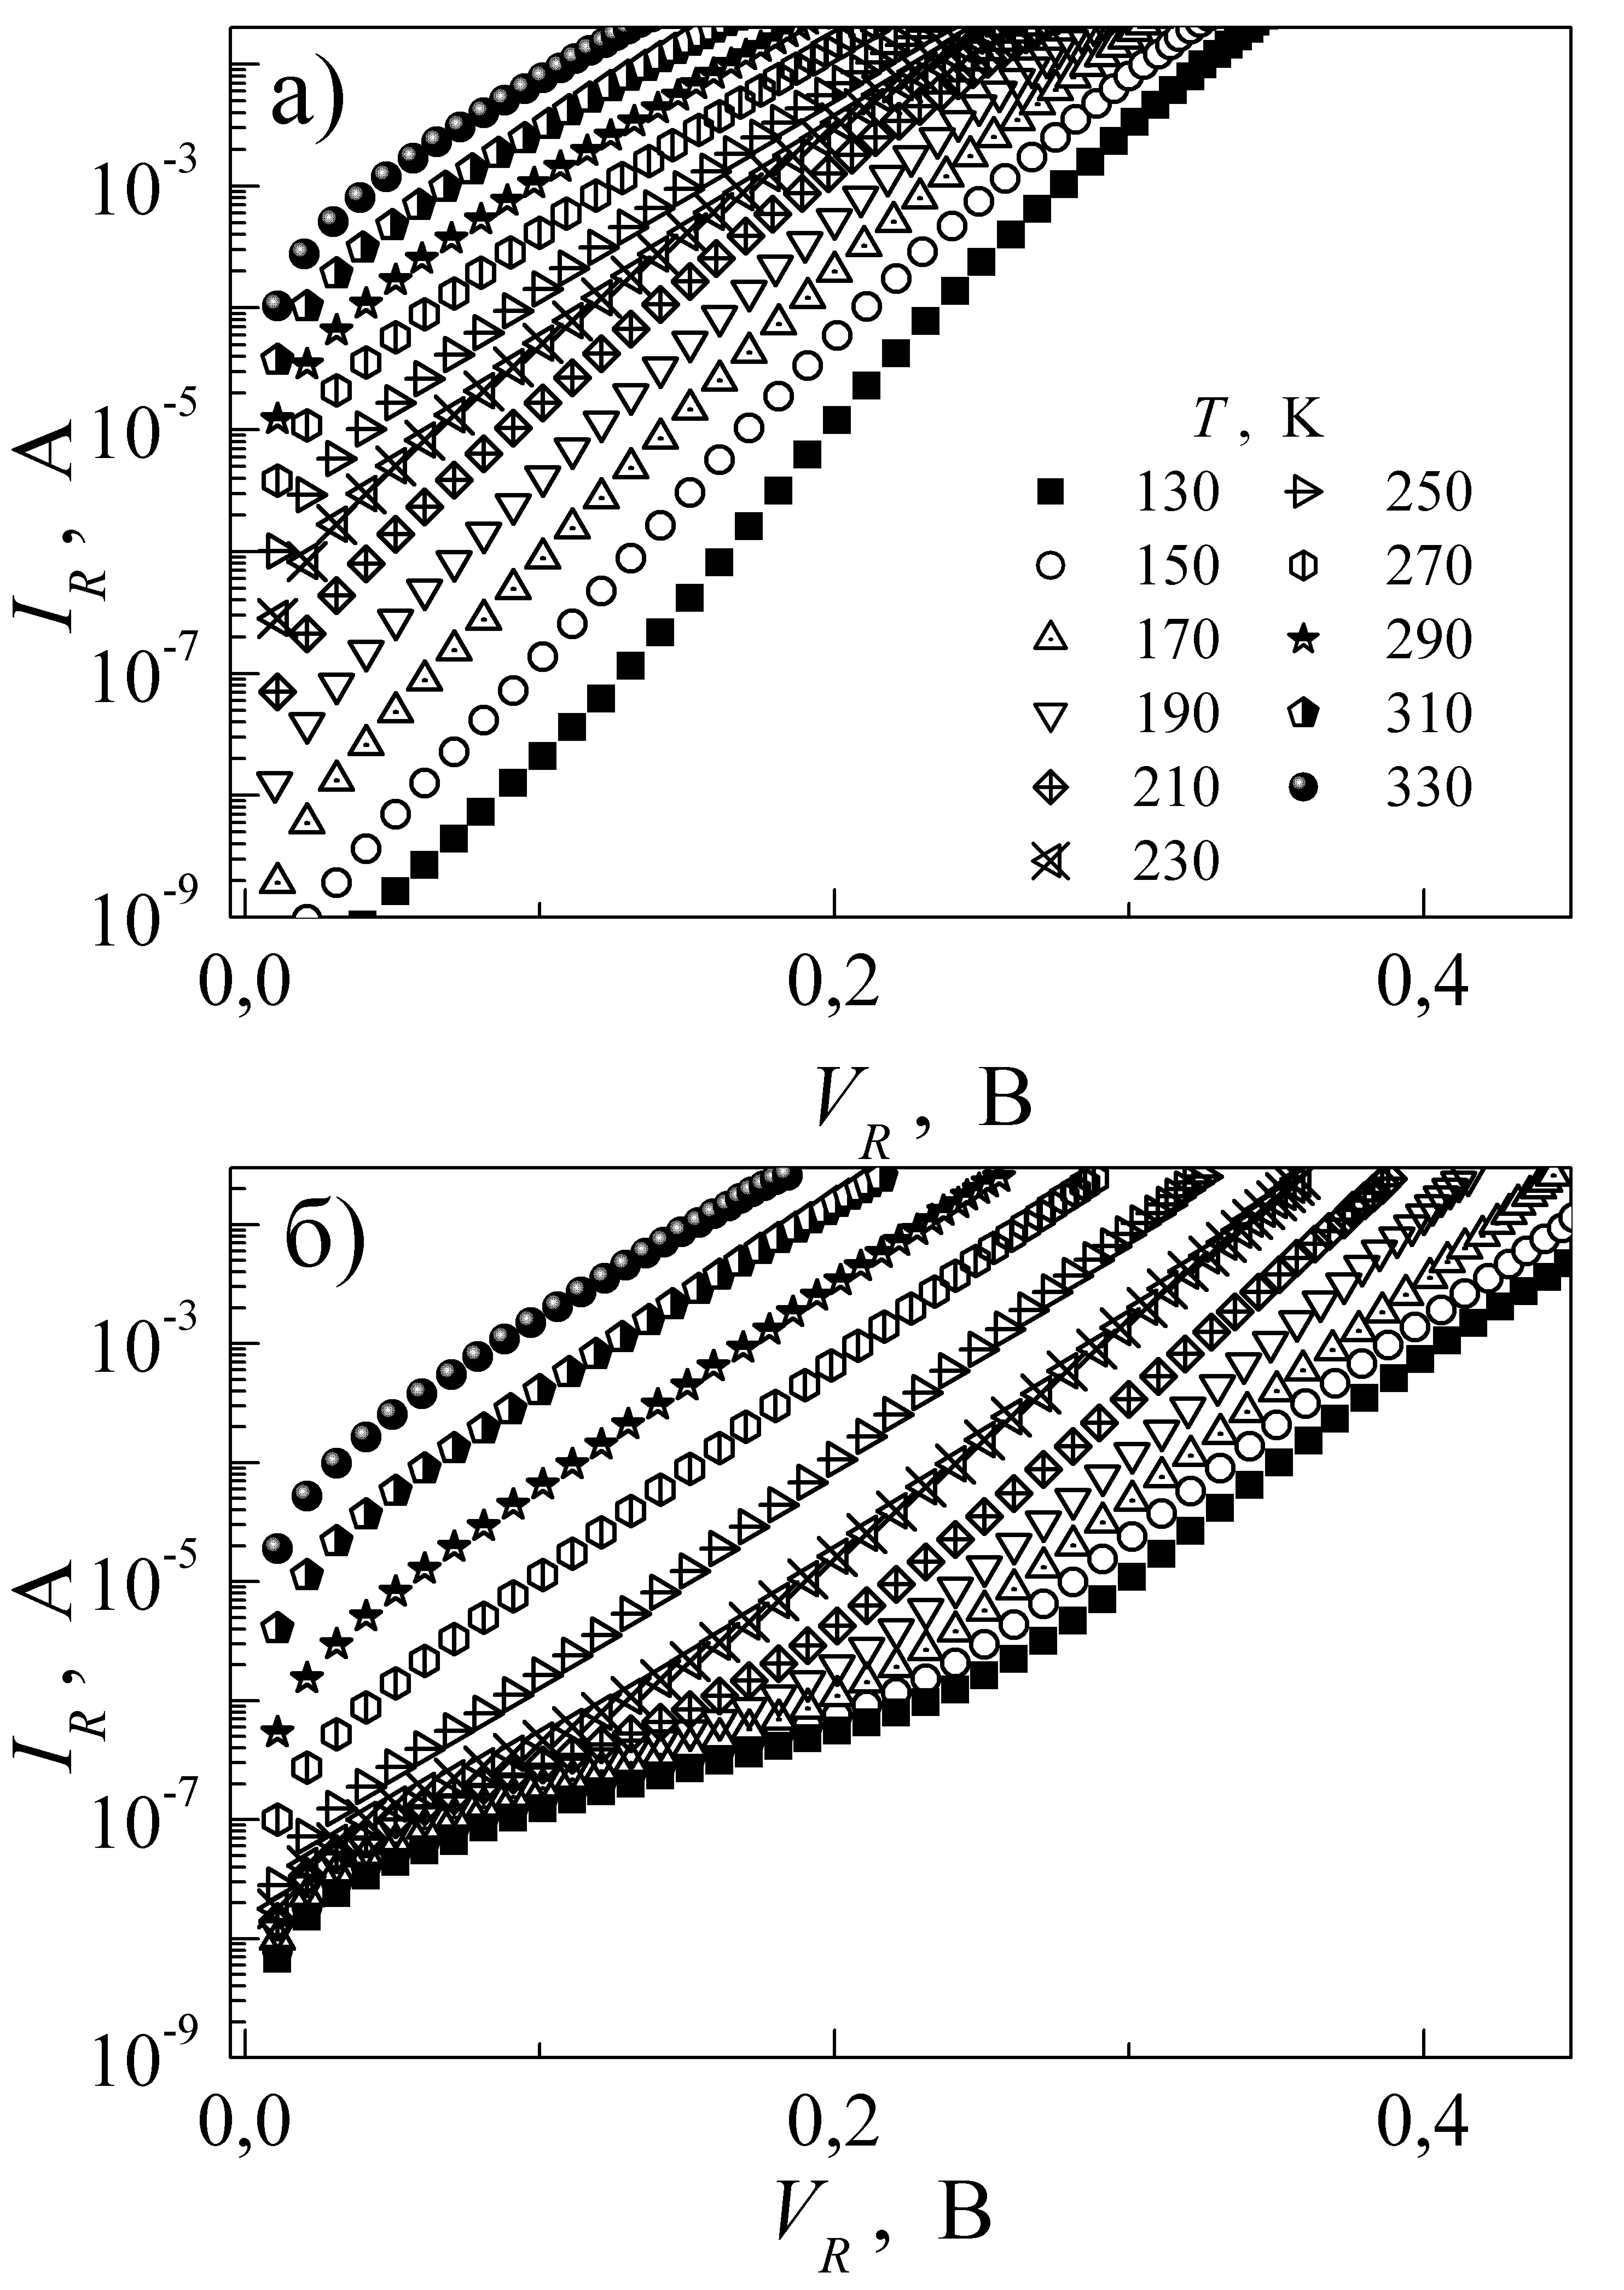
\includegraphics[width=0.6\textwidth]{figIVrad_SDA}
\caption{\label{figIVrad_SDA}
Прямі  ділянки ВАХ структур g6SSDA (a)  та g7SSDA (б) в температурному діапазоні $130\div330$~К.
}%
\end{figure}

Для ВТКС залежність $\log(I)-V$ залишається лінійною і діапазоні струмів близько трьох порядків незалежно від ступеня опромінення.
НТКС структур g6SSDA також є лінійною в напівлогарифмічному масштабі, тоді як при
збільшенні ступеня опромінення суттєво вираженим є вплив послідовного опору.

Для апроксимації ВАХ, як і у випадку неопромінених структур, був використаний вираз (\ref{eqSDA_IV});
для визначення параметрів була застосована процедура, описана в параграфі~\ref{sbMSSi_NonF}.

Температурні залежності ВБШ, обчисленої за формулою~(\ref{eqFb:TE}) для ВТКС, наведено на Рис.~\ref{figFbTrad_SDA}.
Рисунок показує, що висота бар'єру при $\gamma$--опроміненні змінюється немонотонно:
при малих дозах $\Phi_b$ зменшується, тоді як при збільшенні $D$ спостерігається зростання цієї величини і
при $T>200$~К ВБШ при нульовому зміщенні g7SSDA для навіть перевищує відповідне значення для неопромінених структур.
Дозова немонотонність може бути пов'язана зі зміною механізму перенесення заряду після опромінення.
Розглянемо це питання детальніше.

Для g7SSDA при $T>260$~К температурна залежність $\Phi_b$ практично співпадає із залежністю $E_g(T)$ (див. Рис.~\ref{figFbTrad_SDA}),
що співпадає з передбаченнями теорії ТЕ через однорідний бар'єр.
Для ДШ з нижчим ступенем опромінення ВБШ зростає з підвищенням температури, що не може бути поясненим у наближенні цієї теорії.


\begin{figure}
\center
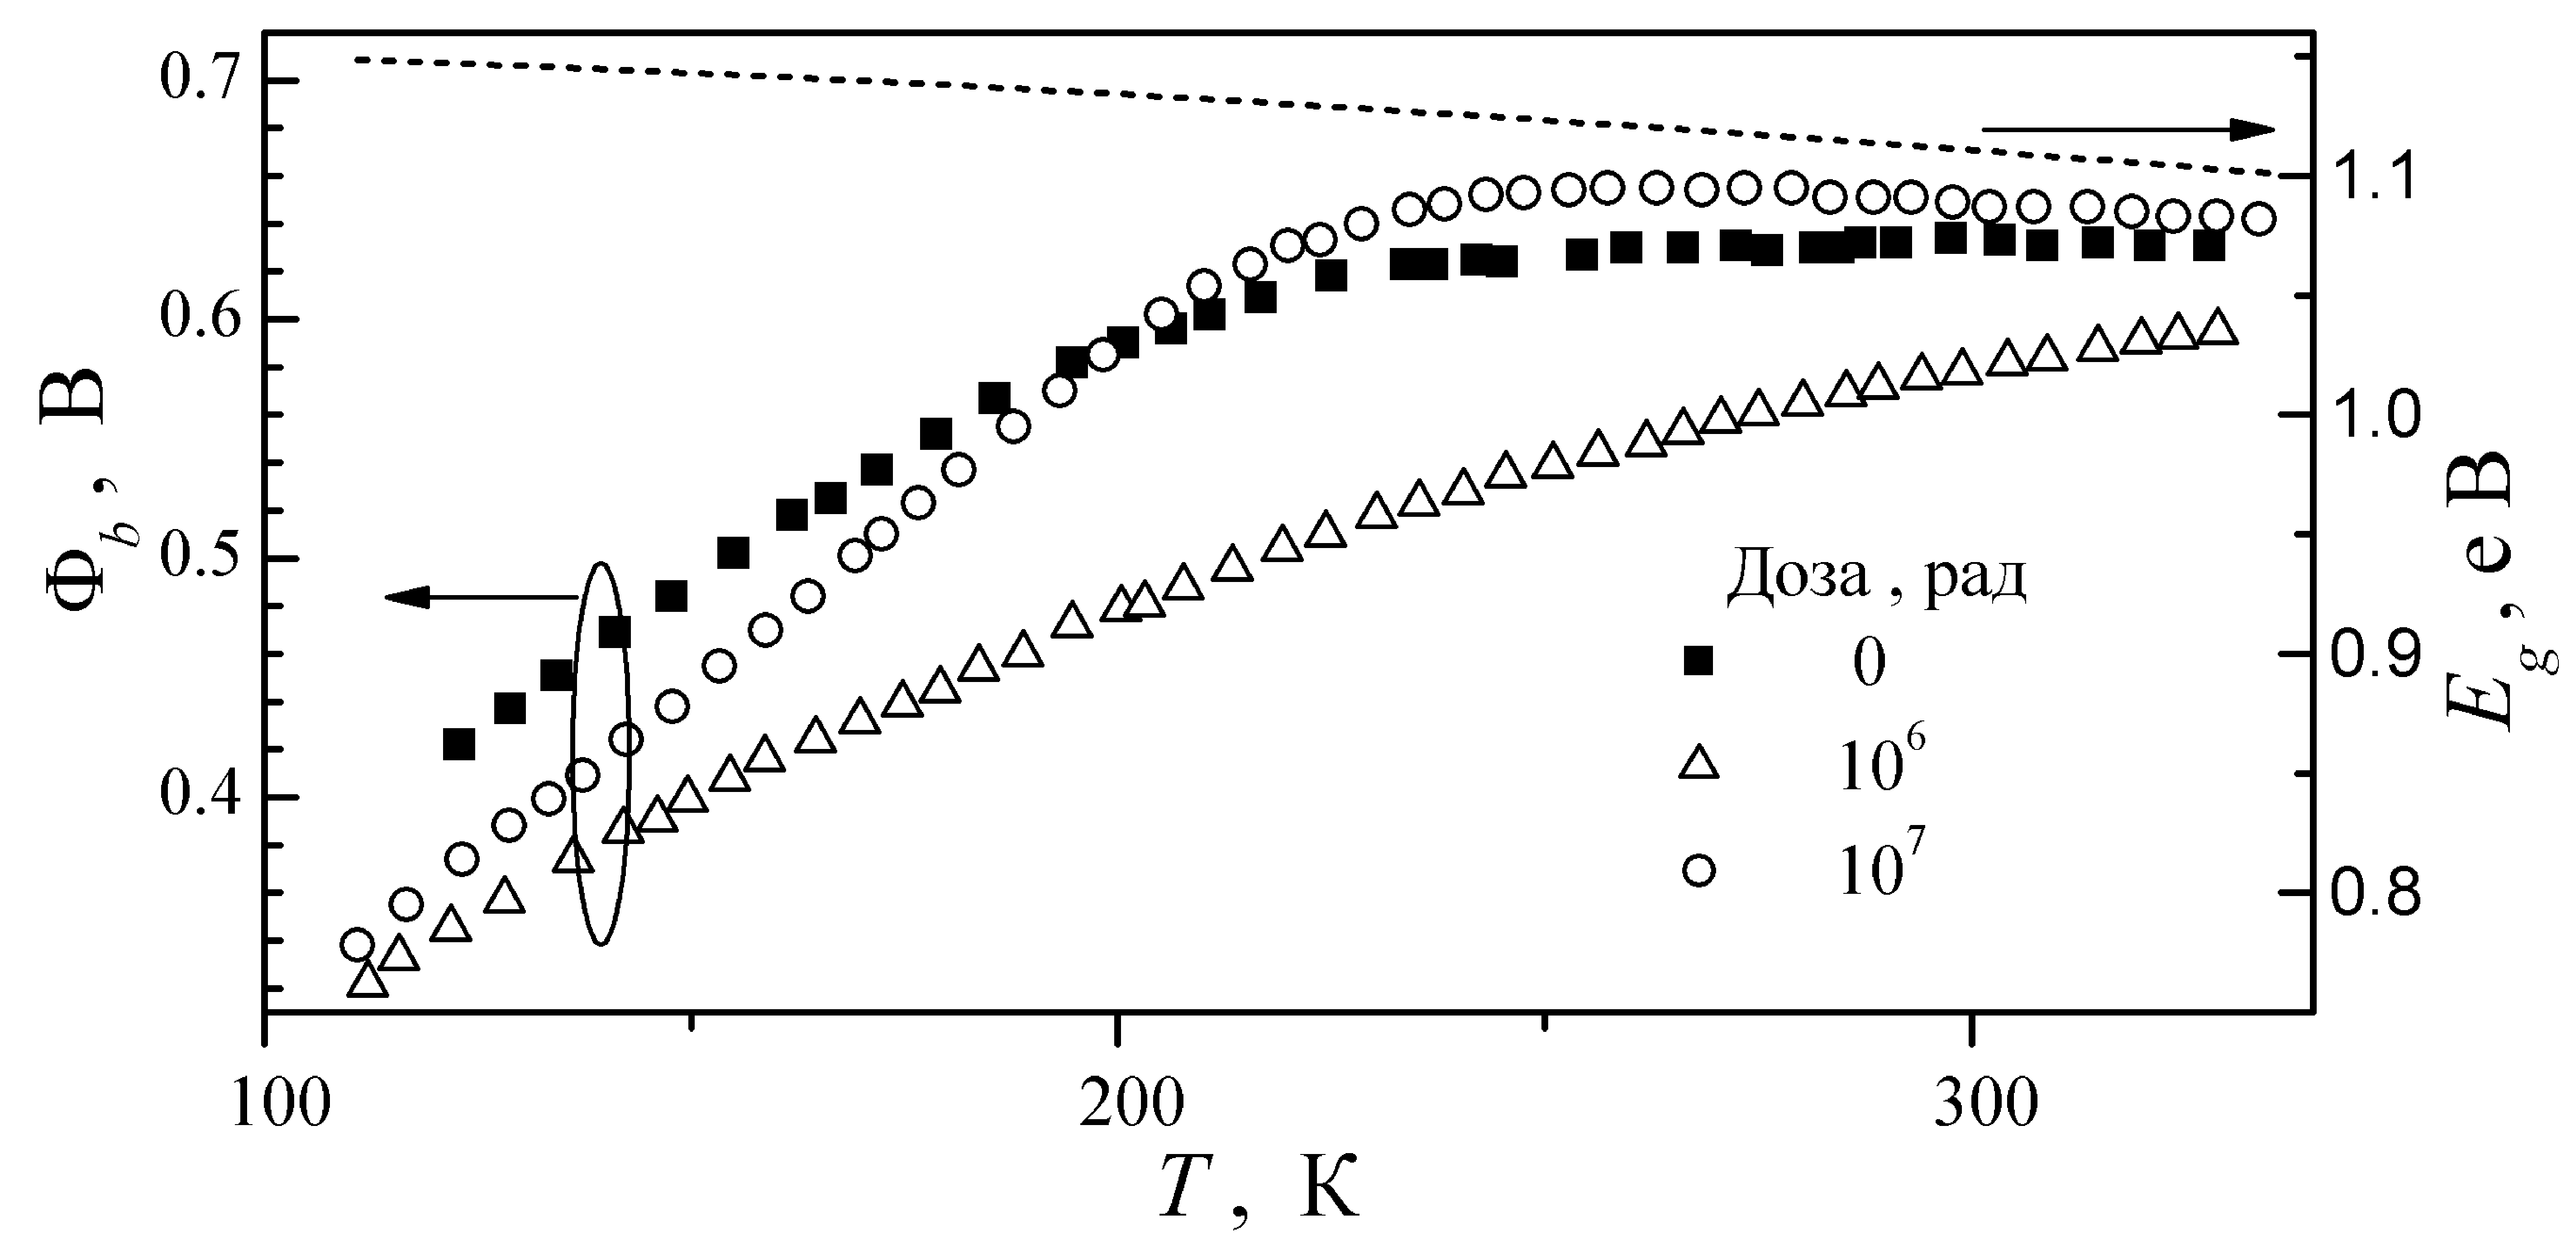
\includegraphics[width=0.9\textwidth]{figFbTrad_SDA}
\caption{\label{figFbTrad_SDA}
Температурні залежності висоти бар'єру, розрахованої в рамках моделі ТЕ та ТПЕ
для ВТКС зразків SSDA (квадрати),
g6SSDA (трикутники) та g7SSDA (кола).
Пунктирна лінія (права вісь)--- залежність ширини забороненої зони кремнію.
}%
\end{figure}


Для оцінки можливого впливу неоднорідності контакту на Рис.~\ref{figFbfbrad_SDA} наведено температурні
залежності  $\Phi_{b}^\mathrm{FB}$, побудовані відповідно до формули~(\ref{eqFbfb}).
На відміну від неопромінених структур, для яких залежність ВБШ в наближенні плоских зон практично співпадала
з поведінкою $E_g$ у всьому температурному діапазоні (див. Рис.~\ref{figFbfb_SDA}),
для g6SSDA  та g7SSDA поведінки $\Phi_{b}^\mathrm{FB}$ та ширини забороненої зони схожі лише при $T>260$~К та $T>240$~К, відповідно.
Отже, лише в цих діапазонах можливе домінування процесів ТЕ і саме для інтервалів температур побудовані
залежності $\Psi_b$ від $q/2kT$, $(n_\mathrm{id}^{-1}-1)$ від $q/2kT$ та $\Psi_b$ від $n_\mathrm{id}$,
представлені на
Рис.~\ref{figFbNrad_SDA}.

\begin{figure}
\center
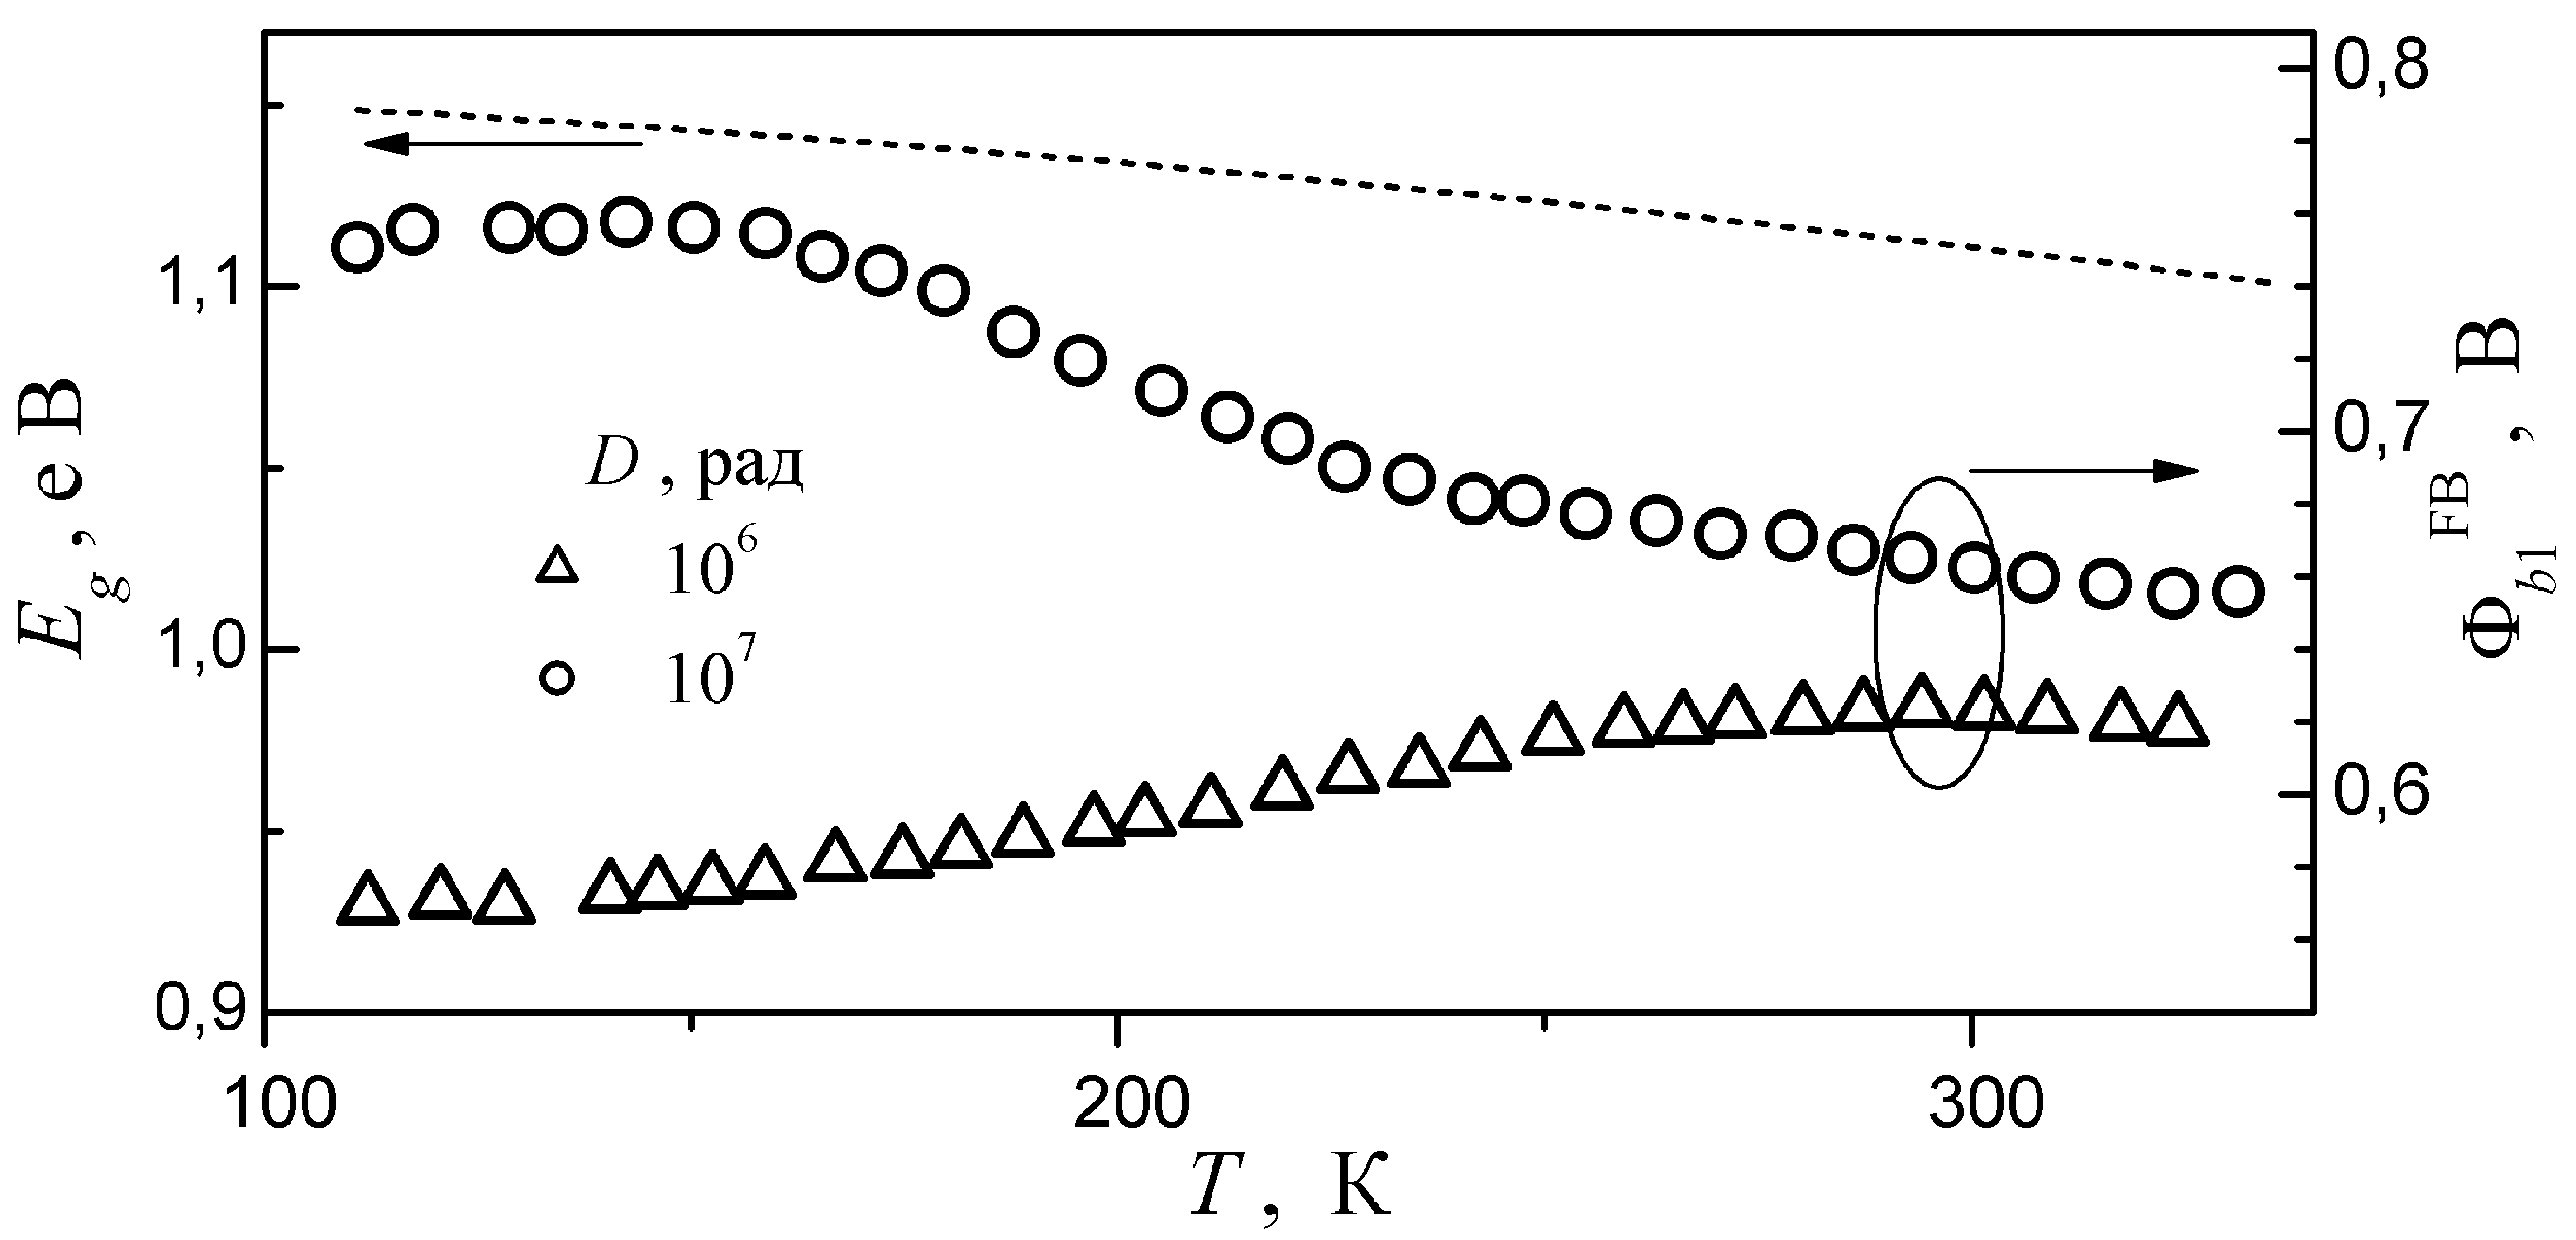
\includegraphics[width=0.8\textwidth]{figFbfbrad_SDA}
\caption{\label{figFbfbrad_SDA}
Температурні залежності ВБШ в наближені плоских зон (точки, права вісь), розрахованої
для ВТКС структур
g6SSDA (трикутники) та g7SSDA (кола),
та ширини забороненої зони (пунктир, ліва вісь).
}%
\end{figure}



\begin{figure}
\center
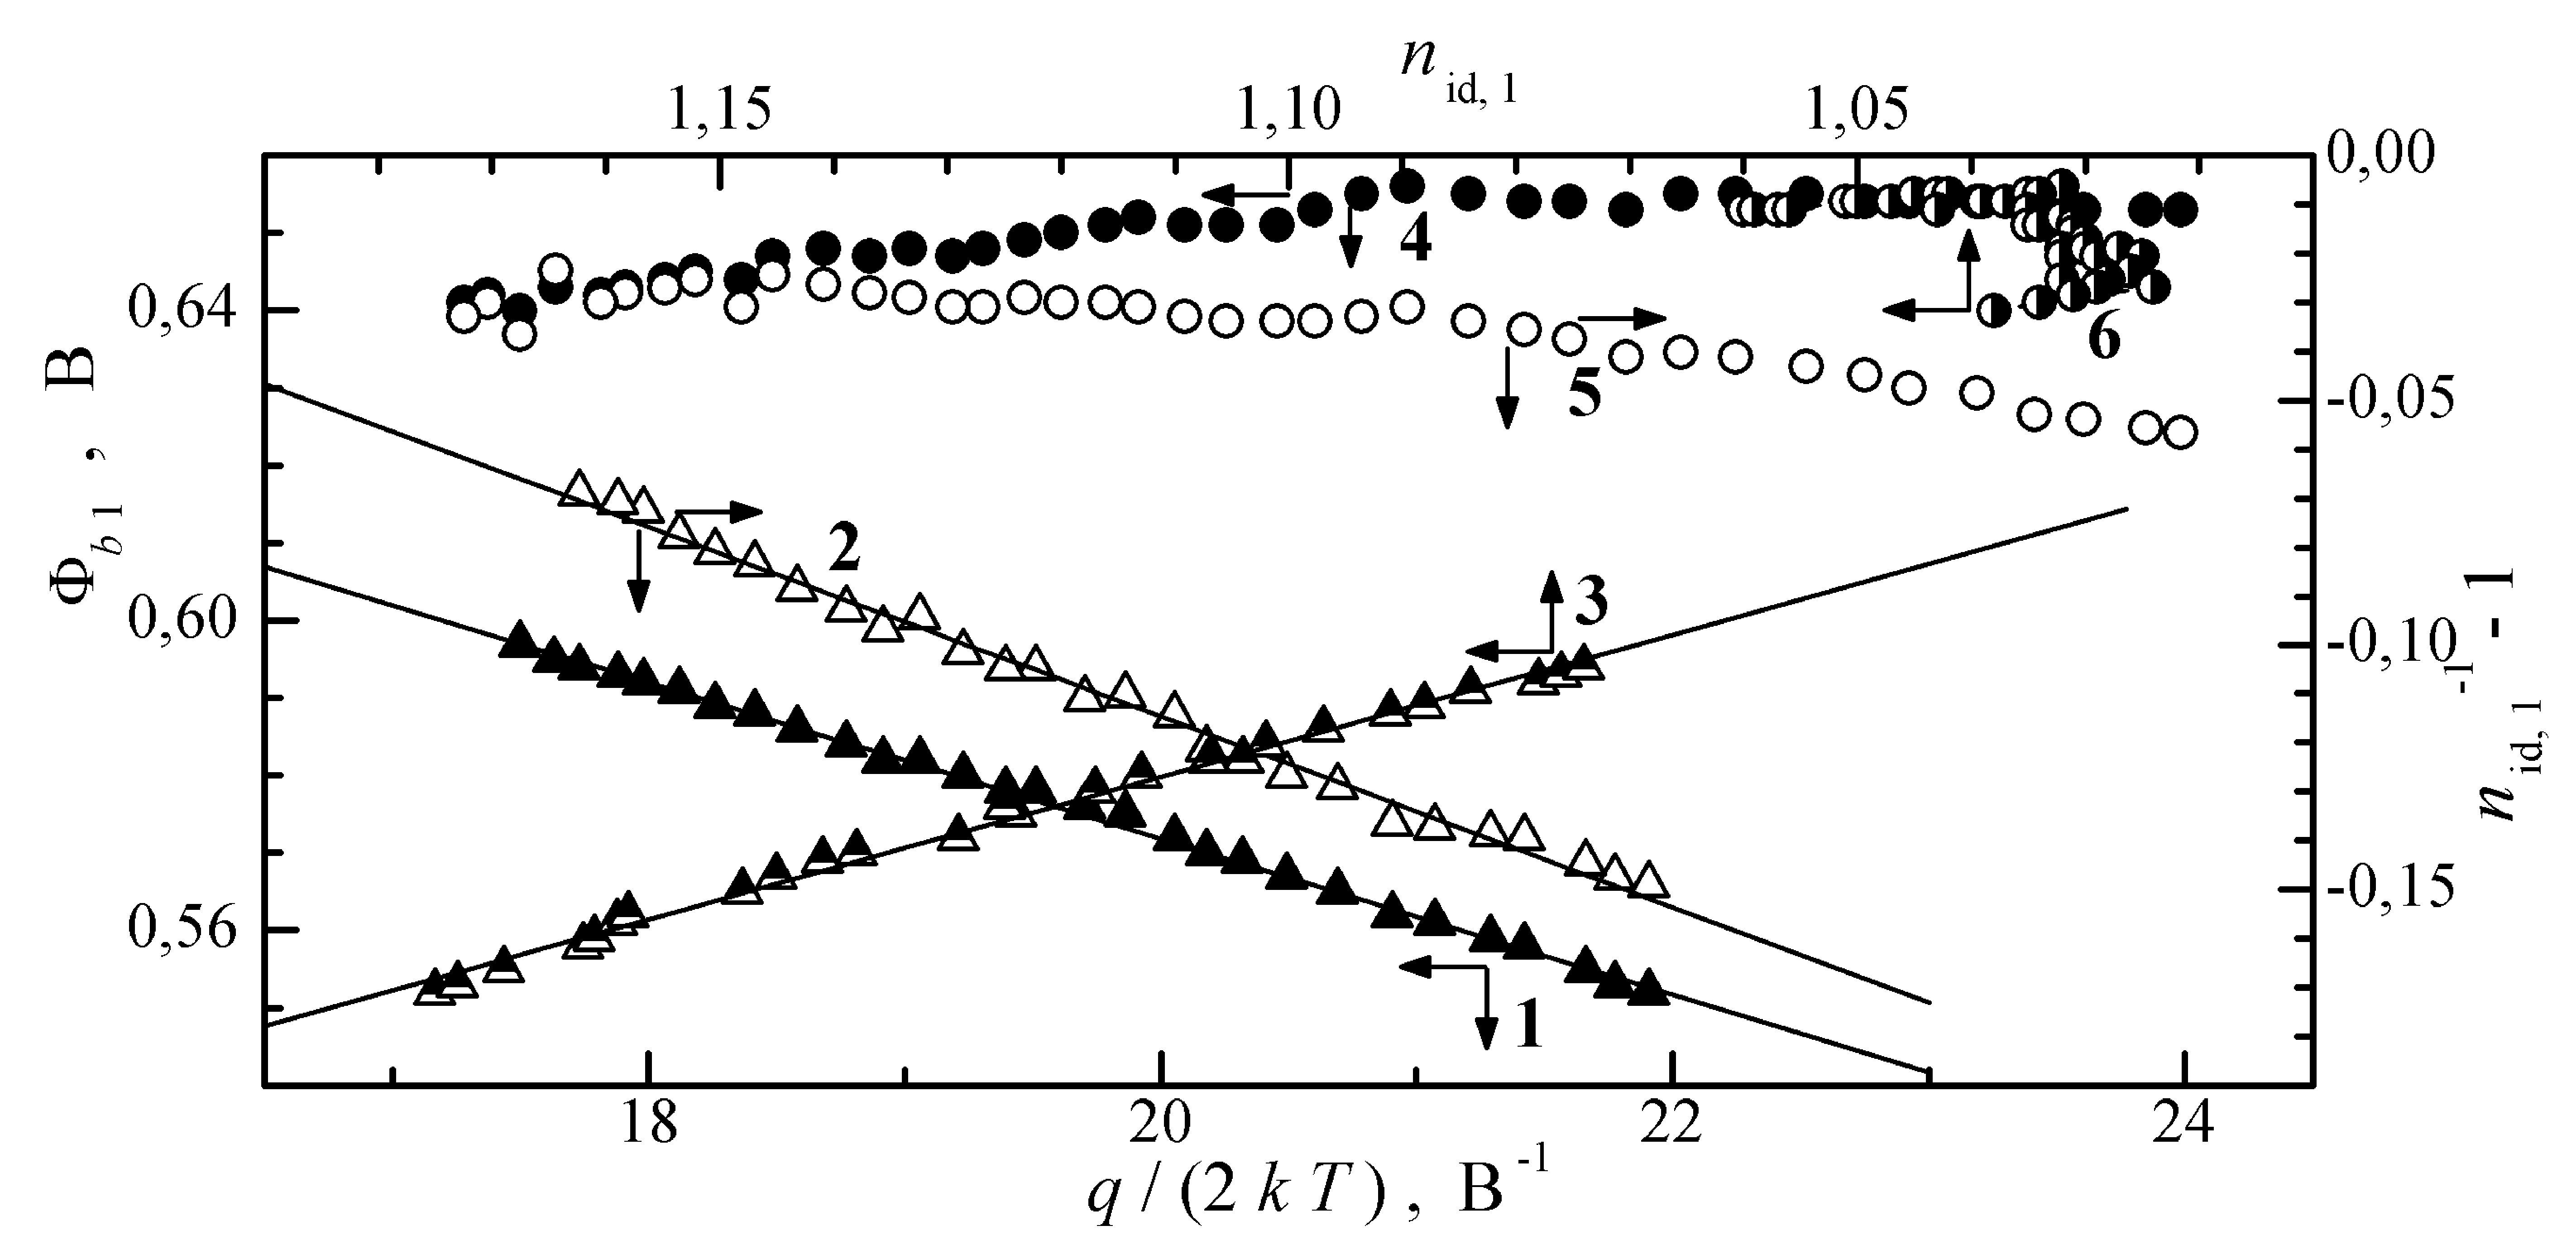
\includegraphics[width=0.9\textwidth]{figFbNrad_SDA}
\caption{\label{figFbNrad_SDA}
Залежності величин $\Phi_{b1}$ (криві 1 та 4, заповнені точки) та
$n_{\mathrm{id},1}^{-1}-1$ (криві 2 та 5, незаповнені точки) від оберненої температури
та залежність ВБШ від фактору неідеальності (криві 3 та 6, напівзаповнені точки)
$D$, рад: 10$^6$ (1--3), 10$^7$ (4--6).
Точки --- експеримент,
прямі --- лінійна апроксимація за методом найменших квадратів.
}%
\end{figure}

Якщо має місце ТЕ через неоднорідний бар'єр, то залежності на Рис.~\ref{figFbNrad_SDA} повинні бути лінійними \cite{Werner,Tung:PhysRev,Schmitsdorf}.
З рисунка видно, що очікуваний вигляд спостерігається лише для g6SSDA,
а отже згаданий механізм є домінуючим в Al$-n-n^+$--Si---Al лише при поглинутій дозі гамма--квантів близько $10^6$~рад при $T>260$~К.
Обчислені в наближені моделі через неоднорідний контакт висота бар'єру за межами патчів,
стандартне відхилення ВБШ та коефіцієнти, які польові залежності розподілу ВБШ наведено в Таблиці~\ref{tabSDAParRad}.
Зауважимо, що отримані дані свідчать про збільшення середнього значення висоти бар'єру та
стандартного відхилення параметрів патчів в опромінених з невеликою дозою $\gamma$--квантів ДШ.

\begin{table}
%\renewcommand{\arraystretch}{1.3}
\caption{Параметри, визначені з ВАХ структур Al$-n-n^+$--Si---Al в наближенні теорії TE}
\label{tabSDAParRad}
\centering
\begin{tabular}{|l|c|c|c|}
\hline
$D$, рад & 0&10$^6$&10$^7$\\ \hline
Діапазон температур, K&230$\div$330&260$\div$330&260$\div$330\\ \hline
$\sigma_{\Phi0}$, мВ&$40\pm5$&$100\pm1$&--\\ \hline
$\rho_2$, $10^{-2}$&$12\pm1$&$27\pm1$&--\\ \hline
$\rho_3$, мВ&$8,0\pm0,3$&$19,0\pm0,4$&--\\ \hline
$\Phi_b^0$, мВ \textsuperscript{ a)}&$663\pm3$&$772\pm2$&--\\ \hline
$\Phi_b^0$, мВ &$662\pm3$ \textsuperscript{ б)}&$772\pm2$ \textsuperscript{ б)}&$710\pm3$ \textsuperscript{ в)}\\ \hline
$\Phi_{b,CV}$, мВ &$683\pm2$&$770\pm5$&$604\pm4$\\ \hline
$A^*$, A$\cdot$см$^{-2}\cdot$K$^{-2}$&$112\pm20$&$115\pm20$&$1200\pm300$\\
\hline
$\Phi_{b,p}$, мВ&$54\pm4$&$74\pm6$&--\\ \hline
$f_p$, $10^{-13}$&$8\pm1$&$8\pm1$&--\\ \hline
\multicolumn{4}{l}{\textsuperscript{ a)} \emph{за залежністю $\Phi_b=f(\frac{1}{2kT})$}} \\
\multicolumn{4}{l}{\textsuperscript{ б)} \emph{за модифікованою залежністю Річардсона (\ref{eqRich:Mod}) }} \\
\multicolumn{4}{l}{\textsuperscript{ в)} \emph{за звичайною залежністю Річардсона (\ref{figRich_SDA})}} \\
\end{tabular}
\end{table}


Для g7SSDA всі залежності на Рис.~\ref{figFbNrad_SDA} не є лінійними, а отже модель ТЕ через неоднорідний бар'єр для цього випадку незастосовна.
Про це свідчать і температурні залежності ВБШ, розраховані для НТКС --- Рис.~\ref{figFb2Trad_SDA}.
У параграфі~\ref{sbMSSi_NonF} вже згадувалося, що поява додаткового струму при низьких температурах у випадку неоднорідного контакту
пов'язана з ефективним проходженням носіїв заряду через патчі, причому висота бар'єру, яка визначається з ВАХ традиційним способом має лінійно зростати з температурою
--- див. вираз (\ref{eqFbFbp}).
Як видно з рисунку, для досліджених структур лінійна залежність спостерігається незалежно від ступеню опромінення.
Проте якщо для g6SSDA обчислені дані свідчать про зростання висоти бар'єру в області патчу та про незмінність загальної площі, яку вони займають (див. Таблицю~\ref{tabSDAParRad}),
то для g7SSDA отримане в рамках моделі від'ємне значення висоти бар'єру $\Phi_{b,p}\approx-9$~мВ не має фізичного змісту.
Тобто, в структурах з високим рівнем опромінення перенесення заряду відбувається в рамках класичного механізму ТЕ.



\begin{figure}
\center
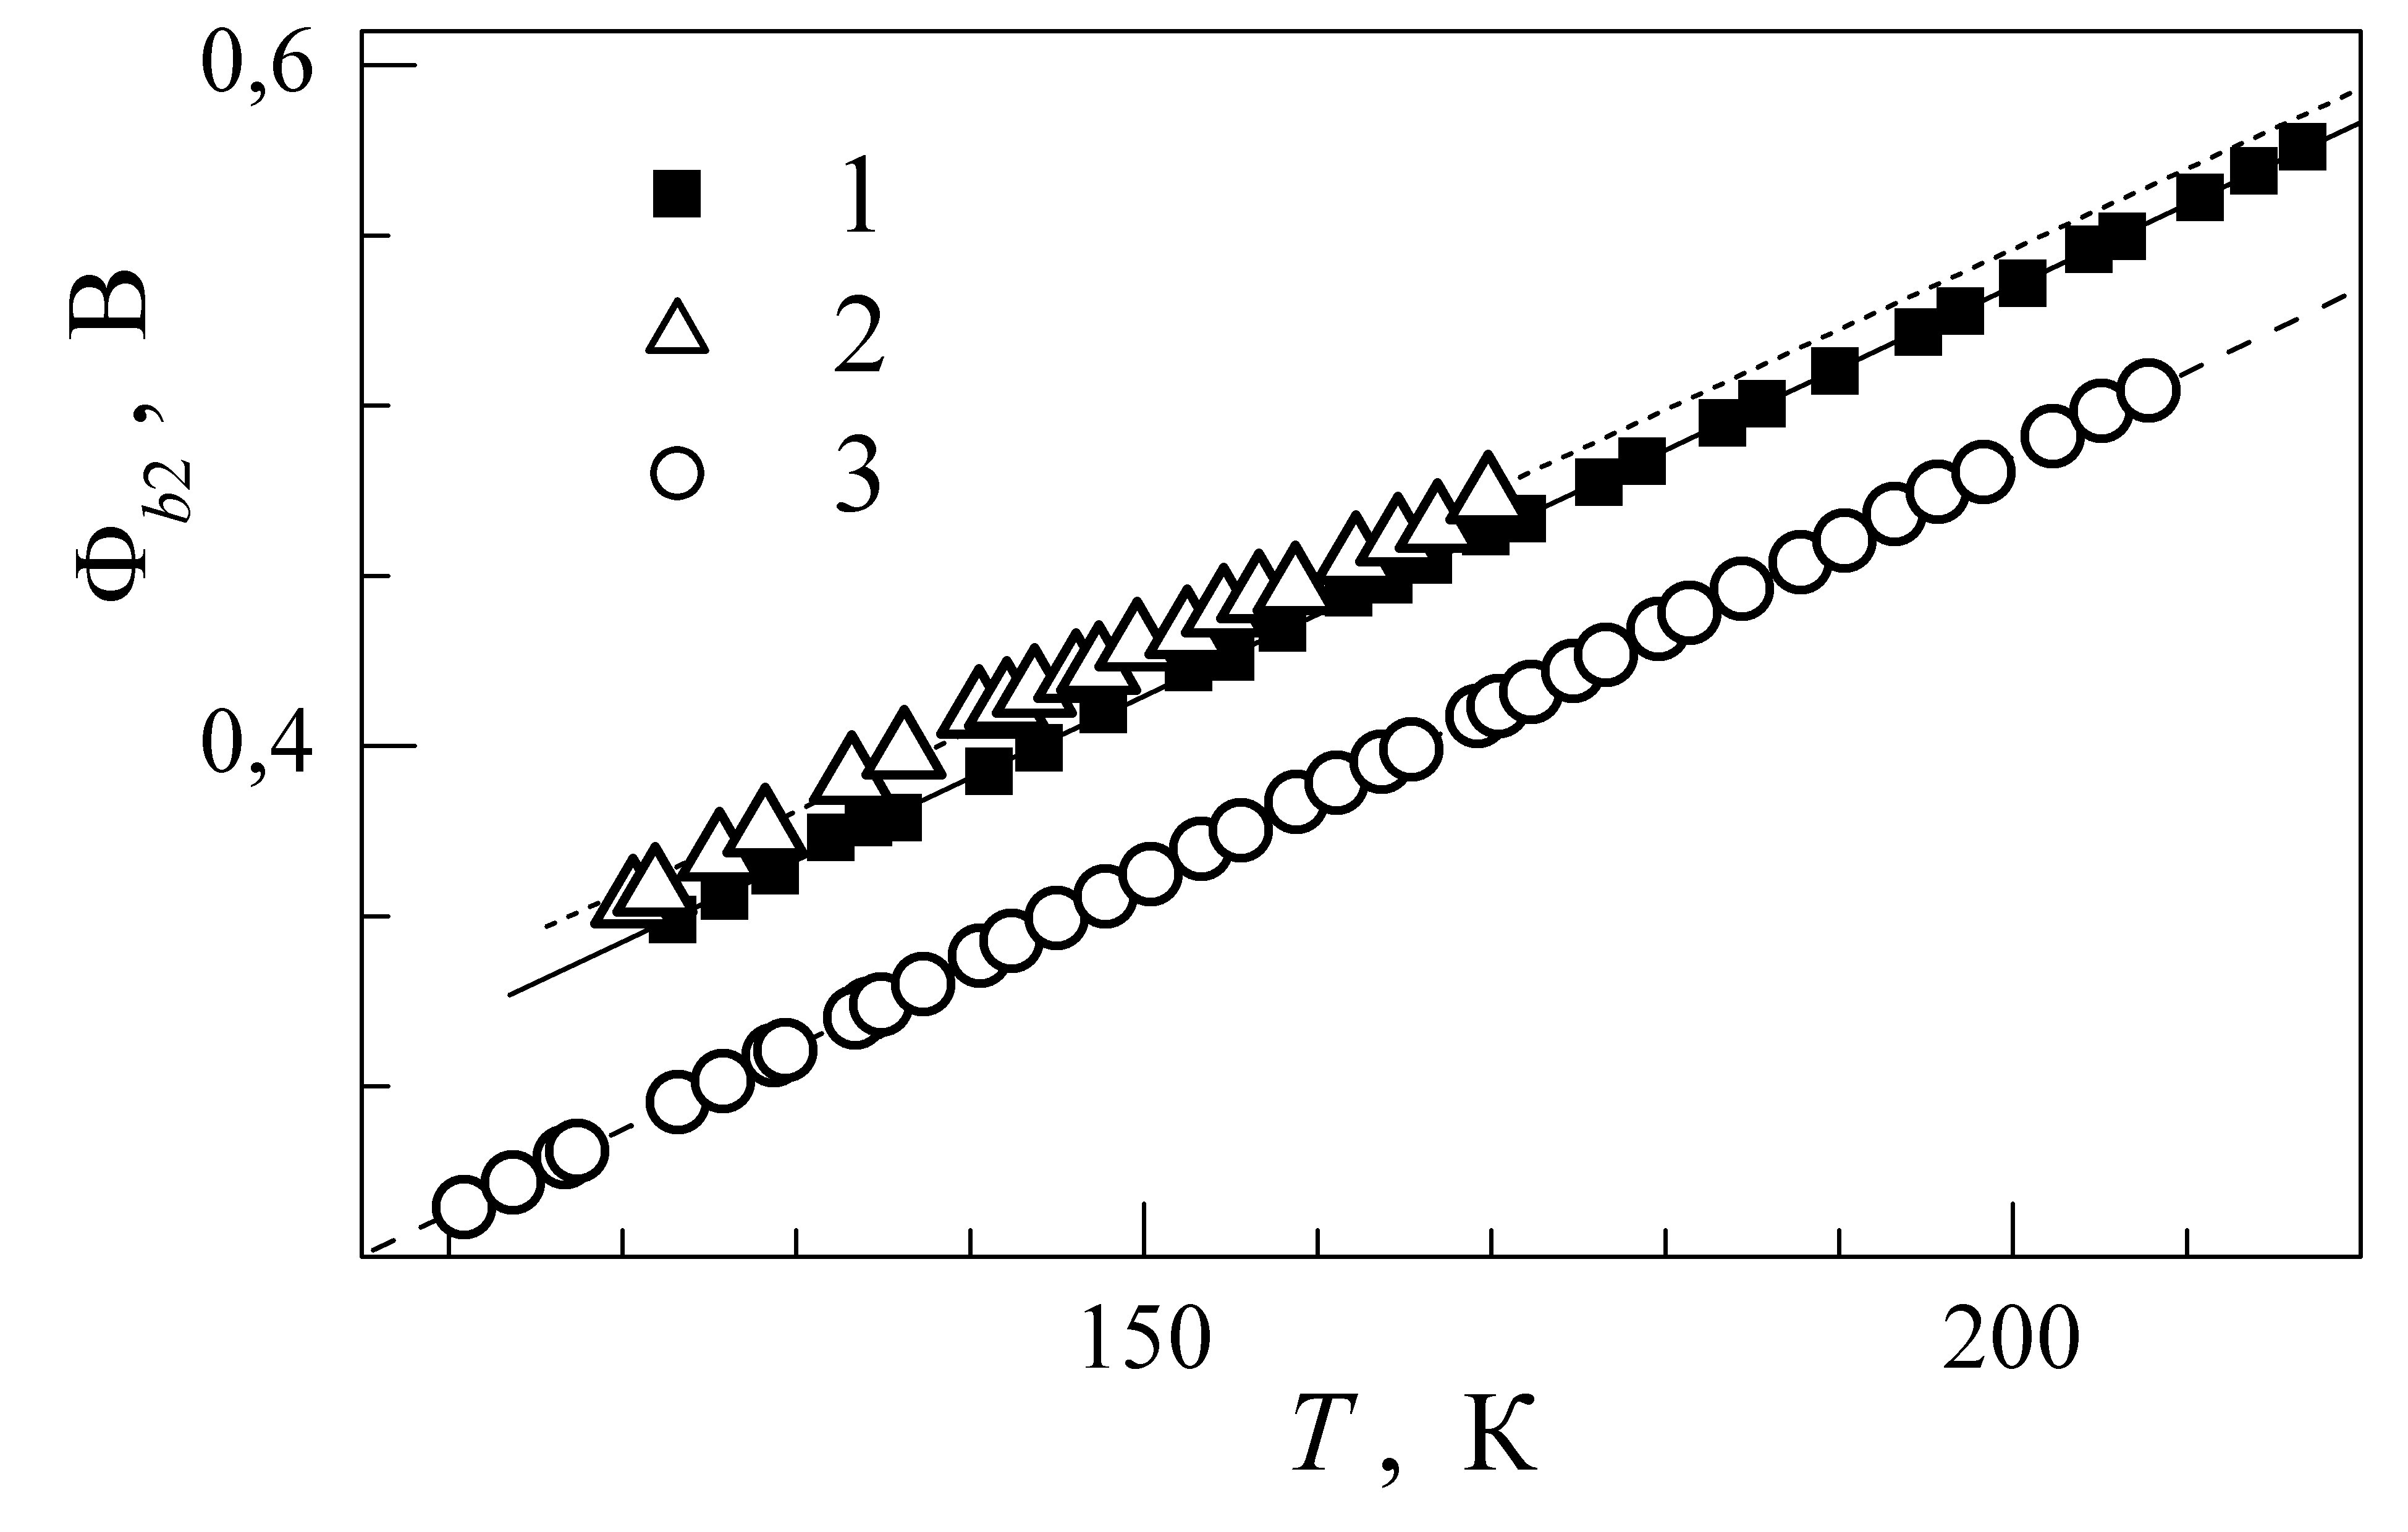
\includegraphics[width=0.65\textwidth]{figFb2Trad_SDA}
\caption{\label{figFb2Trad_SDA}
Температурні залежності висоти бар'єру, розрахованої в рамках моделі ТЕ
для низькотемпературної компоненти струму зразків SSDA (квадрати),
g6SSDA (трикутники) та g7SSDA (кола).
Прямі  --- лінійна апроксимація (суцільна для SSDA, пунктирна для g6SSDA та
штрихована для g7SSDA).
}%
\end{figure}

Спираючись на вищесказане, для оцінки величини $A^*$ для структур з низьким рівнем $\gamma$--опромінення доцільно використовувати
модифіковану залежність Річардсона (Рис.~\ref{figRichMrad_SDA}), тоді як для g7SSDA такий підхід не є виправданим.
На рисунку також наведено звичайну залежність Річардсона для g7SSDA, яка хоч і є лінійною,
проте розраховане за її допомогою значення $A*$ (Таблиця~\ref{tabSDAParRad}) суттєво відрізняється від очікуваного.
Крім того, оцінена таким чином висота бар'єру перевищу значення, отримане з ВФХ, що також суперечить очікуванням,
більш детально розглянутим в параграфі \ref{sbMSSi_NonF}.
Це може свідчити про наявність додаткового, крім ТЕ через однорідний контакт,
механізму перенесення заряду.
Зауважимо, що отримане значення сталої Річардсона для g6SSDA співпадає з відомою з літератури величиною.

З іншого боку, хочеться звернути увагу на те, що згідно з даними Таблиці~\ref{tabSDAParRad},
$\Phi_b^0$ зростає після малих поглинутих доз $\gamma$--опромінення, тоді як подальше збільшення $D$ викликає зменшення
цієї величини.
Така немонотонність співпадає за характером з повідомленою раніше в роботах \cite{Karatas:2006NIMA, Vorobets, Pattabi} і суперечить
даним, отриманим безпосередньо з ВАХ (див. Рис.~\ref{figFbTrad_SDA})  та описаним в \cite{Umana,Verma}.
Таким чином, отримані результати показують, що тип немонотонності зміни висоти бар'єру Шотки (спад--зростанння чи зростання--спад), який спостерігається
при збільшенні дози $\gamma$--опромінення,
залежить від ступеня неоднорідності контакту:
для однорідного інтерфейсу має спостерігатися перший варіант,
тоді як для структур з великим впливом патчів --- другий.


\begin{figure}
\center
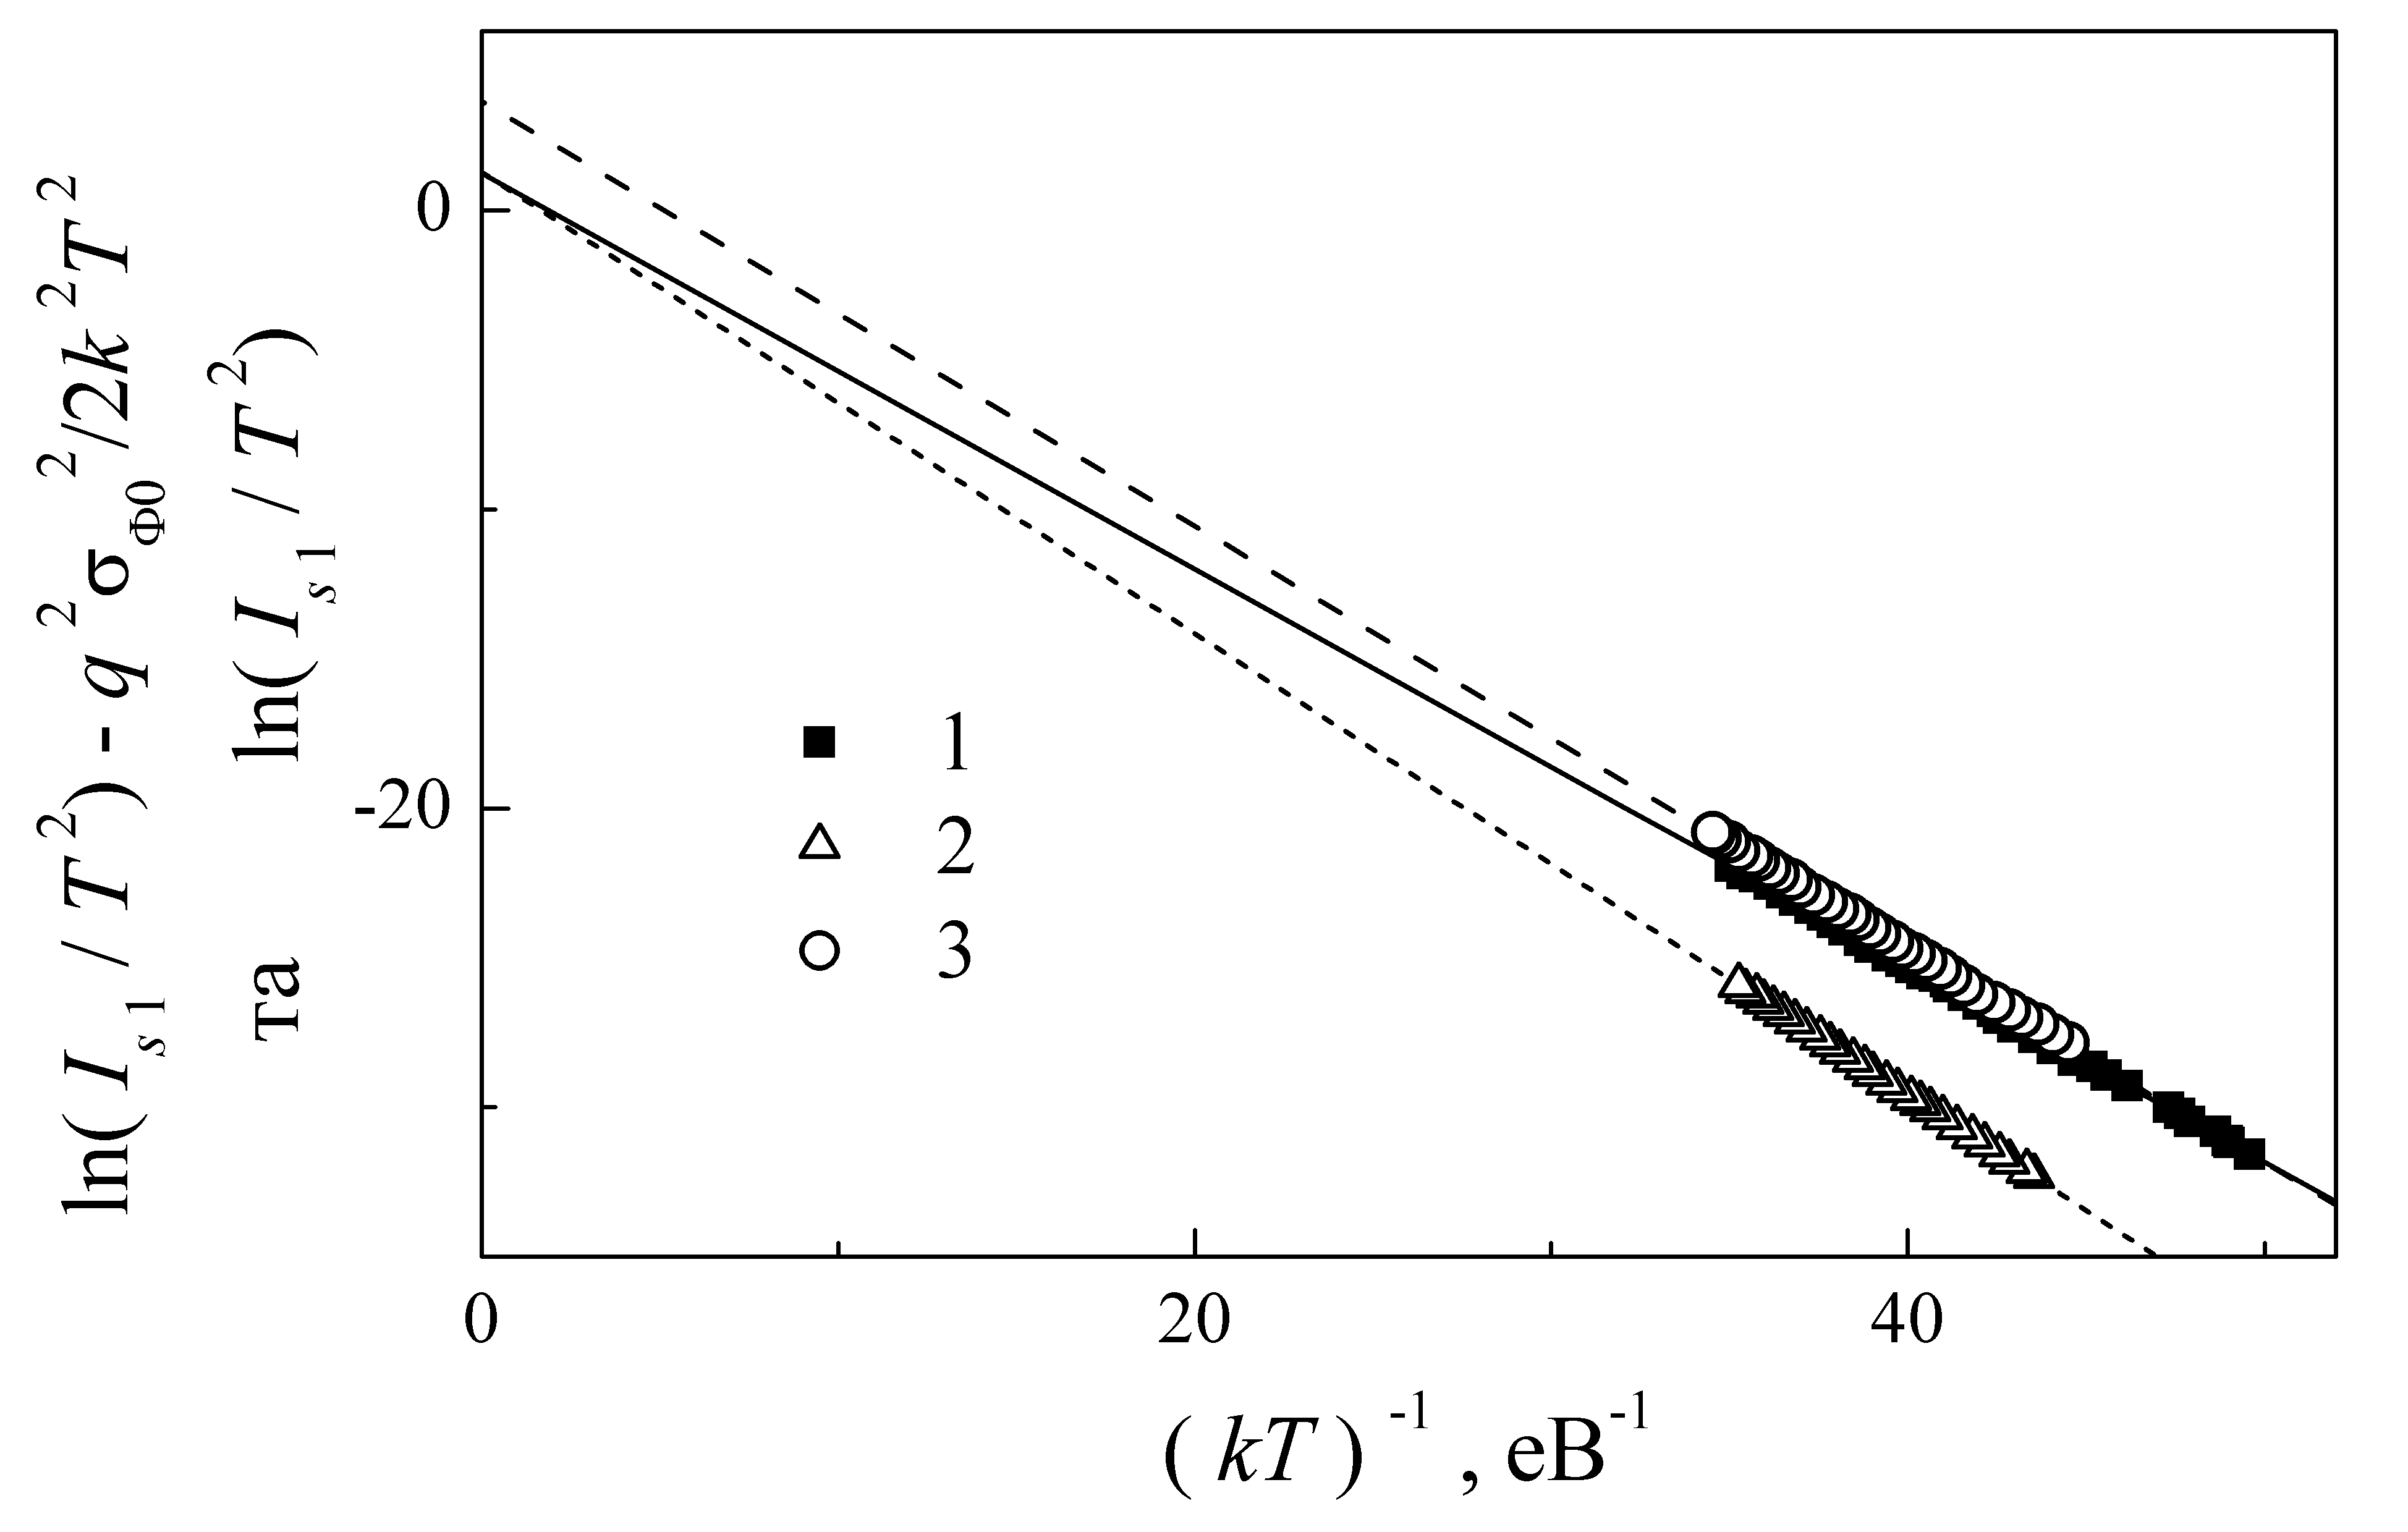
\includegraphics[width=0.7\textwidth]{figRichMrad_SDA}
\caption{\label{figRichMrad_SDA}
Модифіковані (криві 1 та 2, структури SSDA та g6SSDA, відповідно) та звичайні (3, g7SSDA) залежності Річардсона, розраховані для ВТКС в
температурних діапазонах 230$\div$330~K~(1) та 260$\div$330~K~(2, 3).
$\sigma_{\Phi,0}$, мВ: 99 (1) та 100 (2).
Прямі  --- лінійна апроксимація (суцільна для SSDA, пунктирна для g6SSDA та
штрихована для g7SSDA).
}%
\end{figure}

Для визначення механізму перенесення заряду при низьких температурах
в опромінених структурах розглянемо температурні залежні фактору неідеальності --- На Рис.~\ref{figNTrad_SDA}.
Зауважимо, що спостерігається немонотонна дозова залежність зміни $n_\mathrm{id}$.
Представлені результати підтверджують, що для g7SSDA доцільно застосовувати механізм ТЕ при $T>260$~К,
так як в цьому діапазоні температурна залежність $n_\mathrm{id}$ добре описується виразом (\ref{eqN_T:TE})  --- див. Рис.~\ref{figNTrad_SDA}, крива 3.
Водночас з рисунку видно, що для ВТКС структури g6SSDA при $T<260$~К (крива 2), для ВТКС g7SSDA при $T<130$~К (крива 3) та для НТКС g7SSDA (крива 4)
зміни величини фактору неідеальності з підвищенням температури співпадають з передбаченими згідно з формулою (\ref{eqN_T:TFE}) з різними значеннями характеристичної
енергії, наведеними в Таблиці~\ref{tabSDAParRad:DAT}.
Це свідчить на користь наявності тунелювання носіїв заряду.
Зауважимо, що у випадку ТПЕ чи ПЕ величина характеристичної енергії має описуватися
виразом (\ref{eqE00:TFE}),
що для досліджених структур дає величину близько 2~меВ, що набагато менше ніж визначені значення.
Крім того польова емісія є характерною для температур, при яких $kT\approx E_{00}^\mathrm{TFE}$, що не відповідає дослідженому температурному
інтервалу.


\begin{figure}
\center
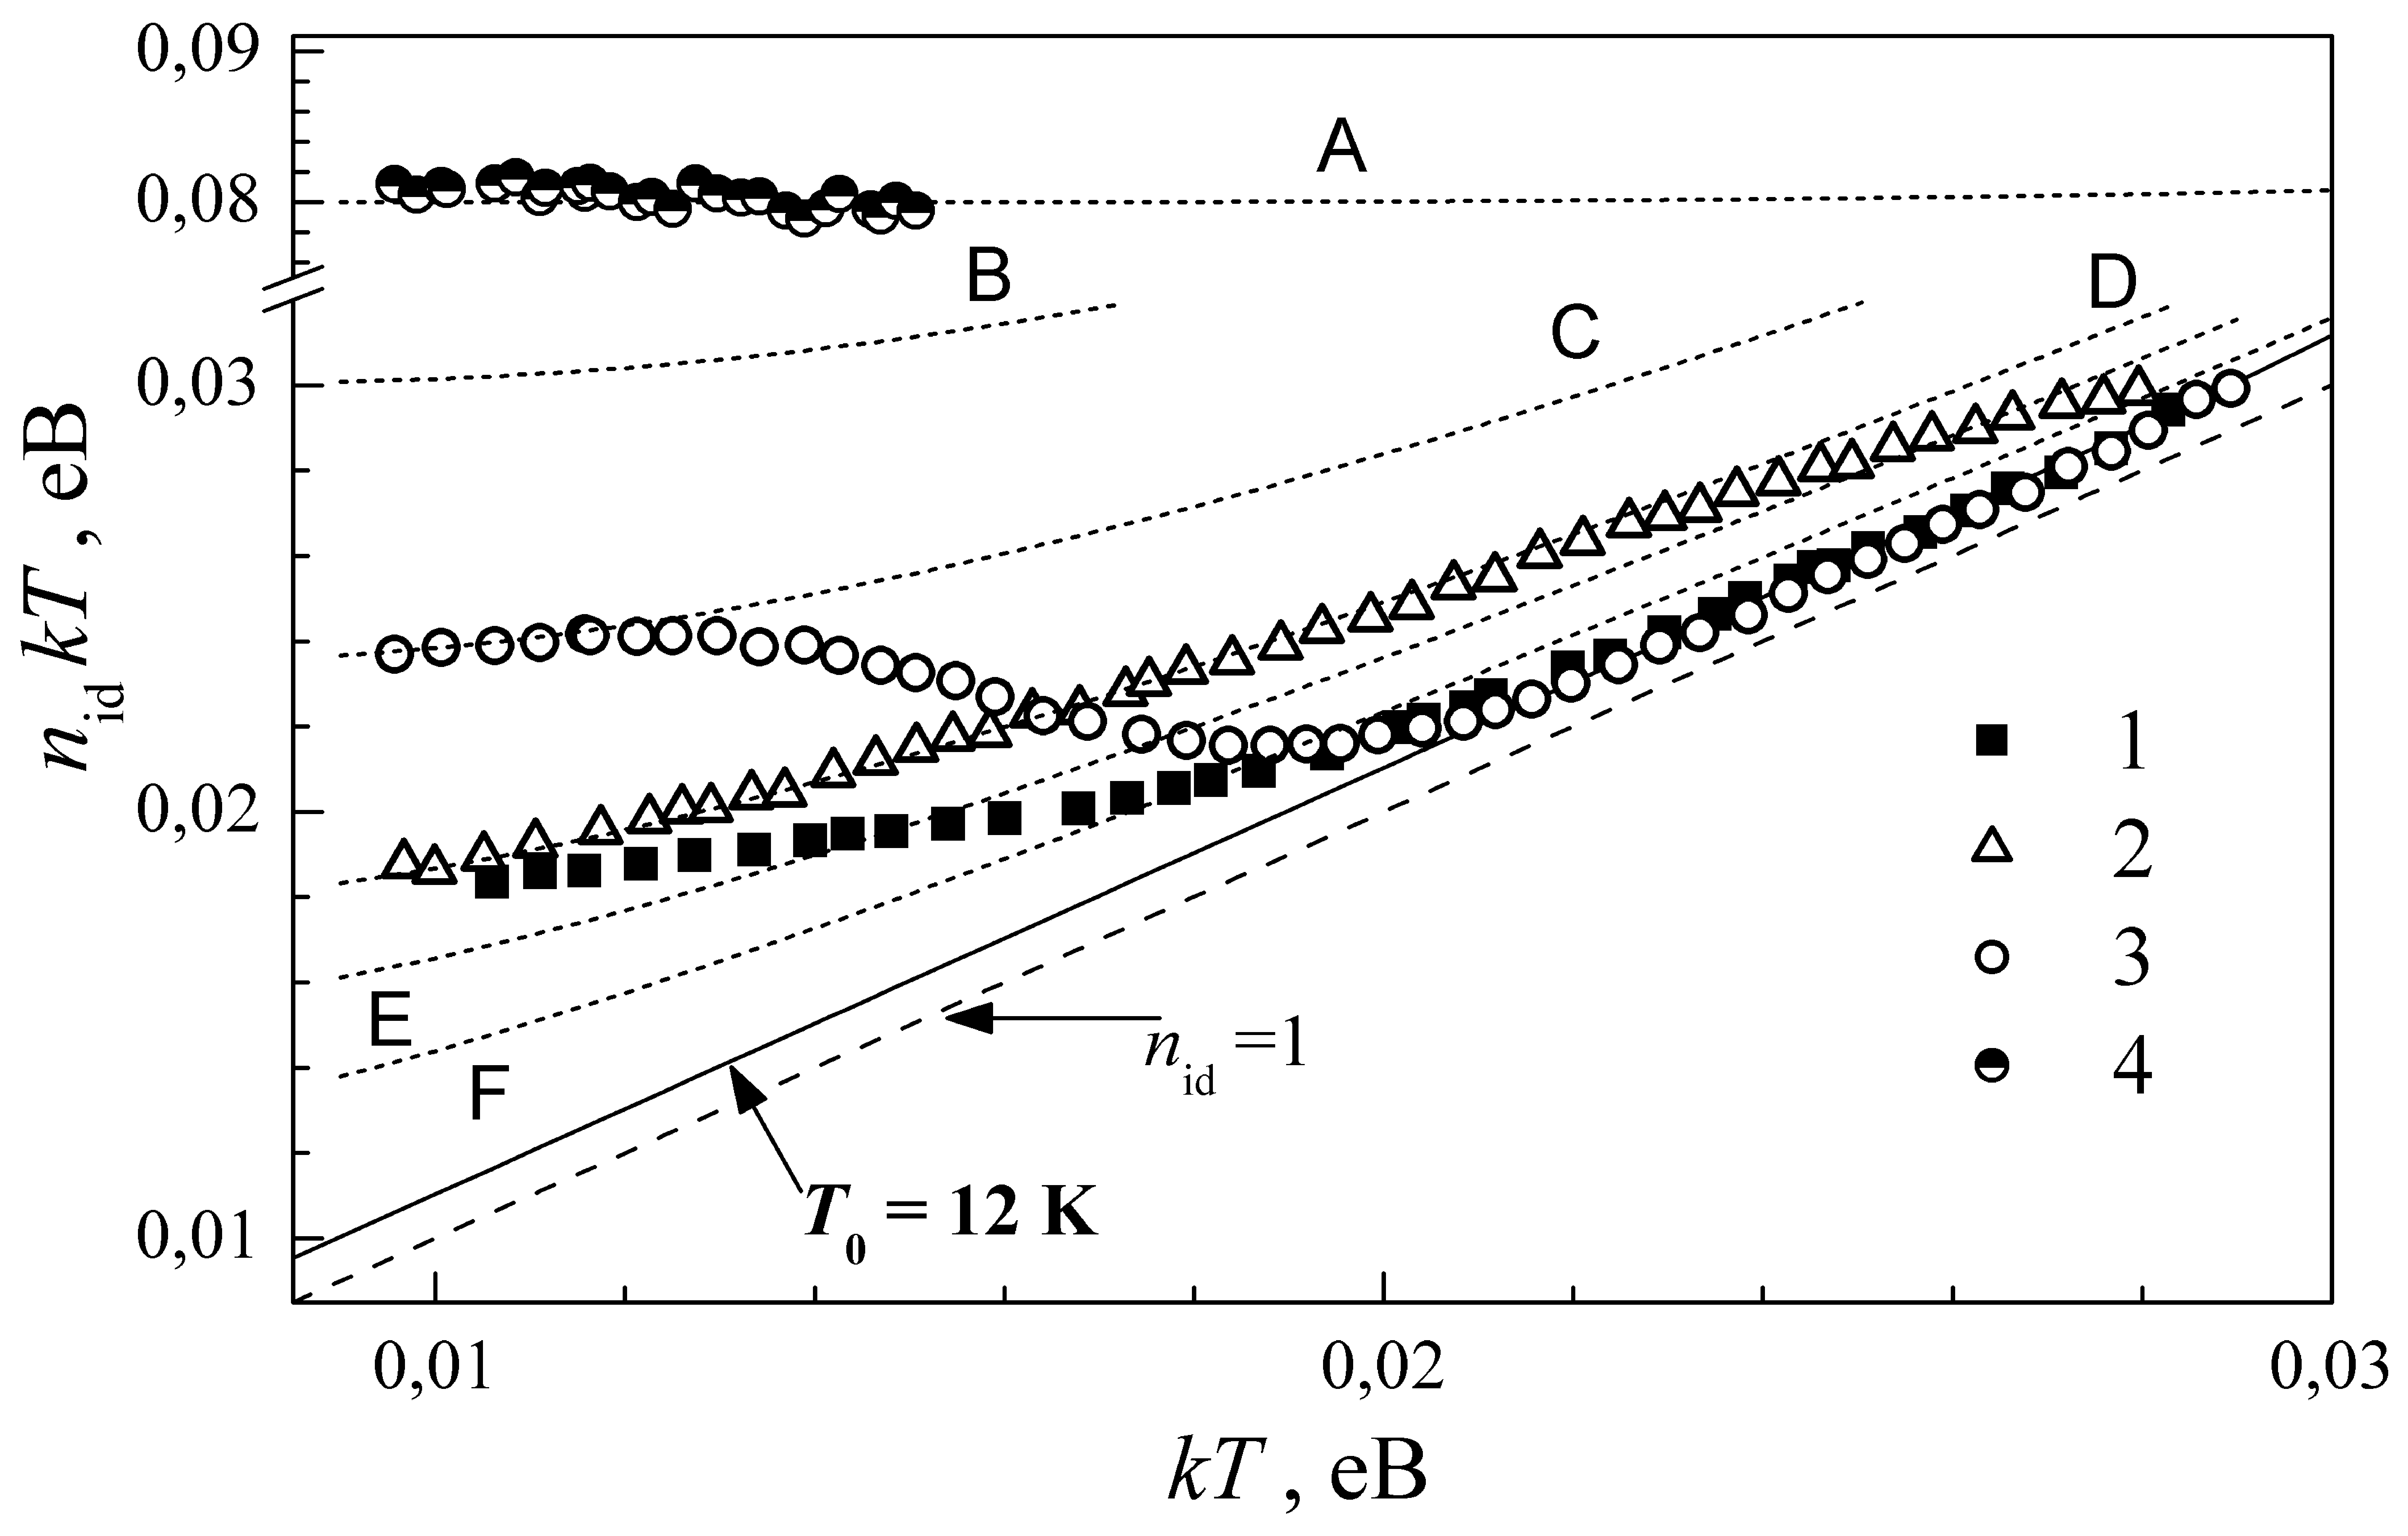
\includegraphics[width=0.75\textwidth]{figNTrad_SDA}
\caption{\label{figNTrad_SDA}
Температурна залежність оберненого нахилу ВАХ для ВТСК (1--3)
та НТСК (4).
$D$, рад: $0$ (1), $10^6$ (2), $10^7$ (3, 4).
Точки --- експеримент,
суцільна лінія розрахована відповідно до формули (\ref{eqN_T:TE}) з $T_0=12$~K,
пунктирні --- з використанням виразу (\ref{eqN_T:TFE}) при
$E_{00}$, меВ: 80 (A), 30 (B), 23.5 (C), 17.8 (D), 15 (E), 12 (F).
Штрихована лінія відповідає ідеальному випадку $n_{\mathrm{id}}=1$.
}%
\end{figure}


\begin{table}
\caption{Параметри, визначені з ВАХ структур Al$-n-n^+$--Si---Al в наближенні теорії DAT}
\label{tabSDAParRad:DAT}
\centering
\begin{tabular}{|l|c|c|c|}
\hline
$D$, рад &10$^6$ \textsuperscript{ a)}&10$^7$ \textsuperscript{ a)}&10$^7$ \textsuperscript{ б)}\\ \hline
Діапазон температур, K&120$\div$240&110$\div$130&110$\div$210\\
$E_{00}$, мВ&$17,8\pm0,5$&$23,5\pm0,5$&$80\pm10$\\
$\chi_\mathrm{calc}$, $10^{-3}$ K$^{-1}$&$39\pm3$&$26\pm2$&$8\pm1$\\
$\chi_\mathrm{fit}$, $10^{-3}$ K$^{-1}$&$73\pm6$&$42\pm4$&$8\pm1$\\
$I_{s0}$, $10^{-14}$A&$5\pm0,5$&$13\pm3$&$(17\pm2)\cdot10^{5}$\\
\hline
\multicolumn{4}{l}{\textsuperscript{ a)}\emph{для високотемпературної компоненти струму}}\\
\multicolumn{4}{l}{\textsuperscript{ б)}\emph{для низькотемпературної компоненти струму}}\\
\end{tabular}
\end{table}

При ТПЕ струм насичення через ДШ описується виразом \cite{Rhoderick1988, Roul}
\begin{equation}\label{eqIs:TFE}
  I_s=\frac{A^*T\sqrt{\pi{E_{00}}(\Phi_b^\mathrm{TFE}-V_n)}}{k\cosh\left(\frac{E_{00}}{kT}\right)}\cdot
  \exp\left[-\frac{V_n}{kT}-\frac{(\Phi_b^\mathrm{TFE}-V_n)}{n_{\mathrm{id}}^\mathrm{T}kT}\right]\,.
\end{equation}
на Рис.~\ref{figFbTrad_SDA} (напівзаповнені трикутники) наведено температурну залежність $\Phi_b^\mathrm{TFE}$, отриману шляхом апроксимації ВАХ структур g6SSDA,
у припущенні, що струм проходить внаслідок ТПЕ.
Наведена залежність відрізняється від поведінки $E_g$.
Таким чином, ні термопольова, ні польова емісії не можуть бути причинами появи ні ВТКС, ні НТКС у досліджених структурах.

З іншого боку,  якщо перенесення заряду відбувається внаслідок багато--стрибкових DAT процесів, то струм насичення має описуватися наступним виразом \cite{Evstropov}:
\begin{eqnarray}
  I_s&=&I_{s0}\exp(\chi\,T) \label{eqIs:DAT}\,,\\
   \chi&=&\frac{\beta+k\ln(N_c/N_d)}{E_{00}}\,, \label{eqKsi:Dat}
\end{eqnarray}
де
$I_{s0}$ залежить, зокрема, від концентрації дефектів,
$\beta$ --- температурний коефіцієнт зниження $\Phi_b$.

На Рис.~\ref{figIsTrad_SDA} наведено температурні залежності струмів насичення, визначених для досліджених структур.
З рисунка видно, що між $\ln I_s$ та $T$ спостерігається лінійна залежність саме в тих температурних діапазонах,
де значення фактору неідеальності описується виразом, також характерним для DAT.


\begin{figure}
\center
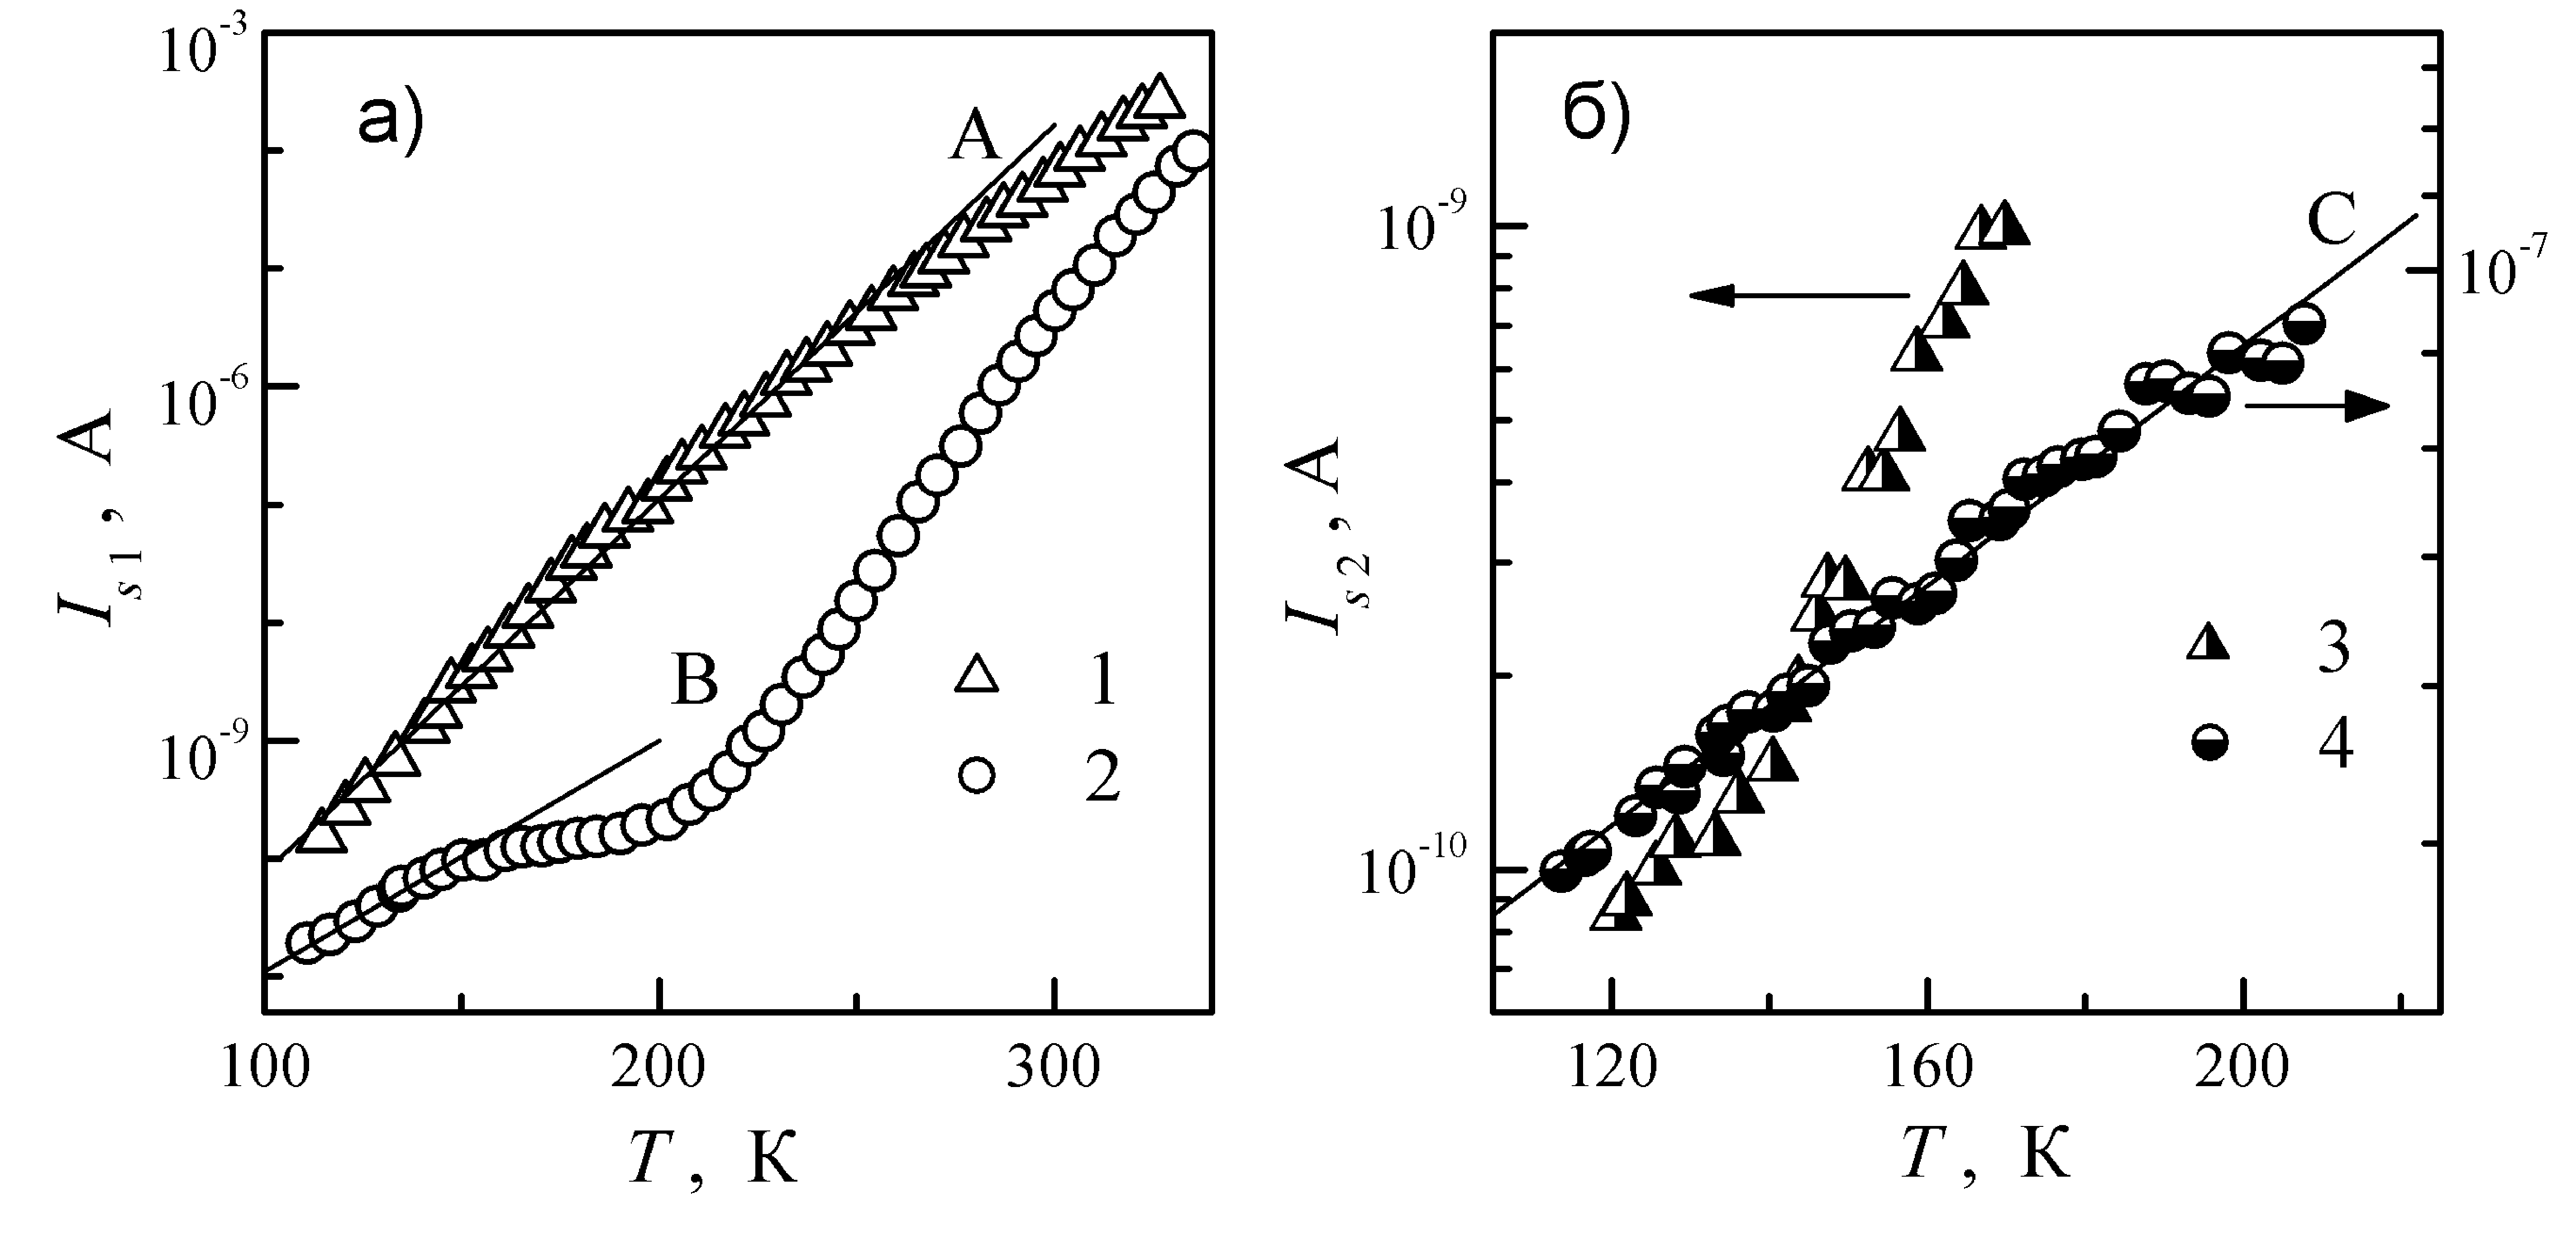
\includegraphics[width=0.9\textwidth]{figIsTrad_SDA}
\caption{\label{figIsTrad_SDA}
Температурні залежності струму насичення ВТКС (а, незаповнені точки)
та НТКС (б, напівзаповнені точки).
$D$, рад: 10$^6$~(1, 3, трикутники), 10$^7$~(2, 4, кола).
Лінії розраховані за формулою (\ref{eqIs:DAT}).
$\chi$, $10^{-3}$~K$^{-1}$: 73~(A), 42~(B), 26~(C).
$I_s$, A: $5\cdot10^{-14}$~(A),
$1,3\cdot10^{-13}$~(B),
$1,7\cdot10^{-8}$~(C).
}%
\end{figure}

Використовуючи вираз (\ref{eqKsi:Dat}), значення $\beta=0,26$~меВ/K \cite{Aboelfotoh, Evstropov} та величини $E_{00}$,
отримані із залежностей $n_\mathrm{id}=f(T)$ (Рис.~\ref{figNTrad_SDA}),
були розраховані значення $\chi_\mathrm{calc}$ для g6SSDA та g7SSDA, наведені в Таблиці~\ref{tabSDAParRad:DAT}.
Ця таблиця також містить величини $\chi_\mathrm{fit}$, отримані шляхом апроксимації залежностей $I_s$ з використанням виразу~(\ref{eqIs:DAT}).
Як видно з наведених даних, величини, отримані різними способами, не дуже суттєво відрізняються одна від одної.
Цей збіг, а також температурні залежності $I_s$ та $n_\mathrm{id}$ свідчать,
що ВТКС в g6SSDA при $T=120\div240$~K, ВТКС в g7SSDA при $T<130$~K і НТКС в g7SSDA визначаються процесами багато--стрибкового DAT.






\subsection{Зворотній струм у $\gamma$--опромінених кремнієвих діодах Шотки}

Приклади зворотних ВАХ досліджуваних структур при низьких та високих температурах наведено на Рис.~\ref{figIV_SDArRad}.
Видно, що $\gamma$--опромінення з низькою дозою
\begin{enumerate}[label=\asbuk*),leftmargin=0em,itemindent=1.5em]
\item залишає майже незмінною величину зворотного струму поблизу азотних температур;
\item в декілька разів підвищує величину $I_R$ в околі кімнатних температур;
\item практично не впливає на польову залежність зворотного струму.
\end{enumerate}
У ДШ зі збільшеною поглинутою дозою при низьких зміщеннях спостерігається збільшення струму в області низьких температур і зворотній ефект при високих;
водночас при великих зміщеннях ($V_R>2$~В) він практично перестає залежати від температури, зростаючи при цьому приблизно на порядок.


\begin{figure}
\center
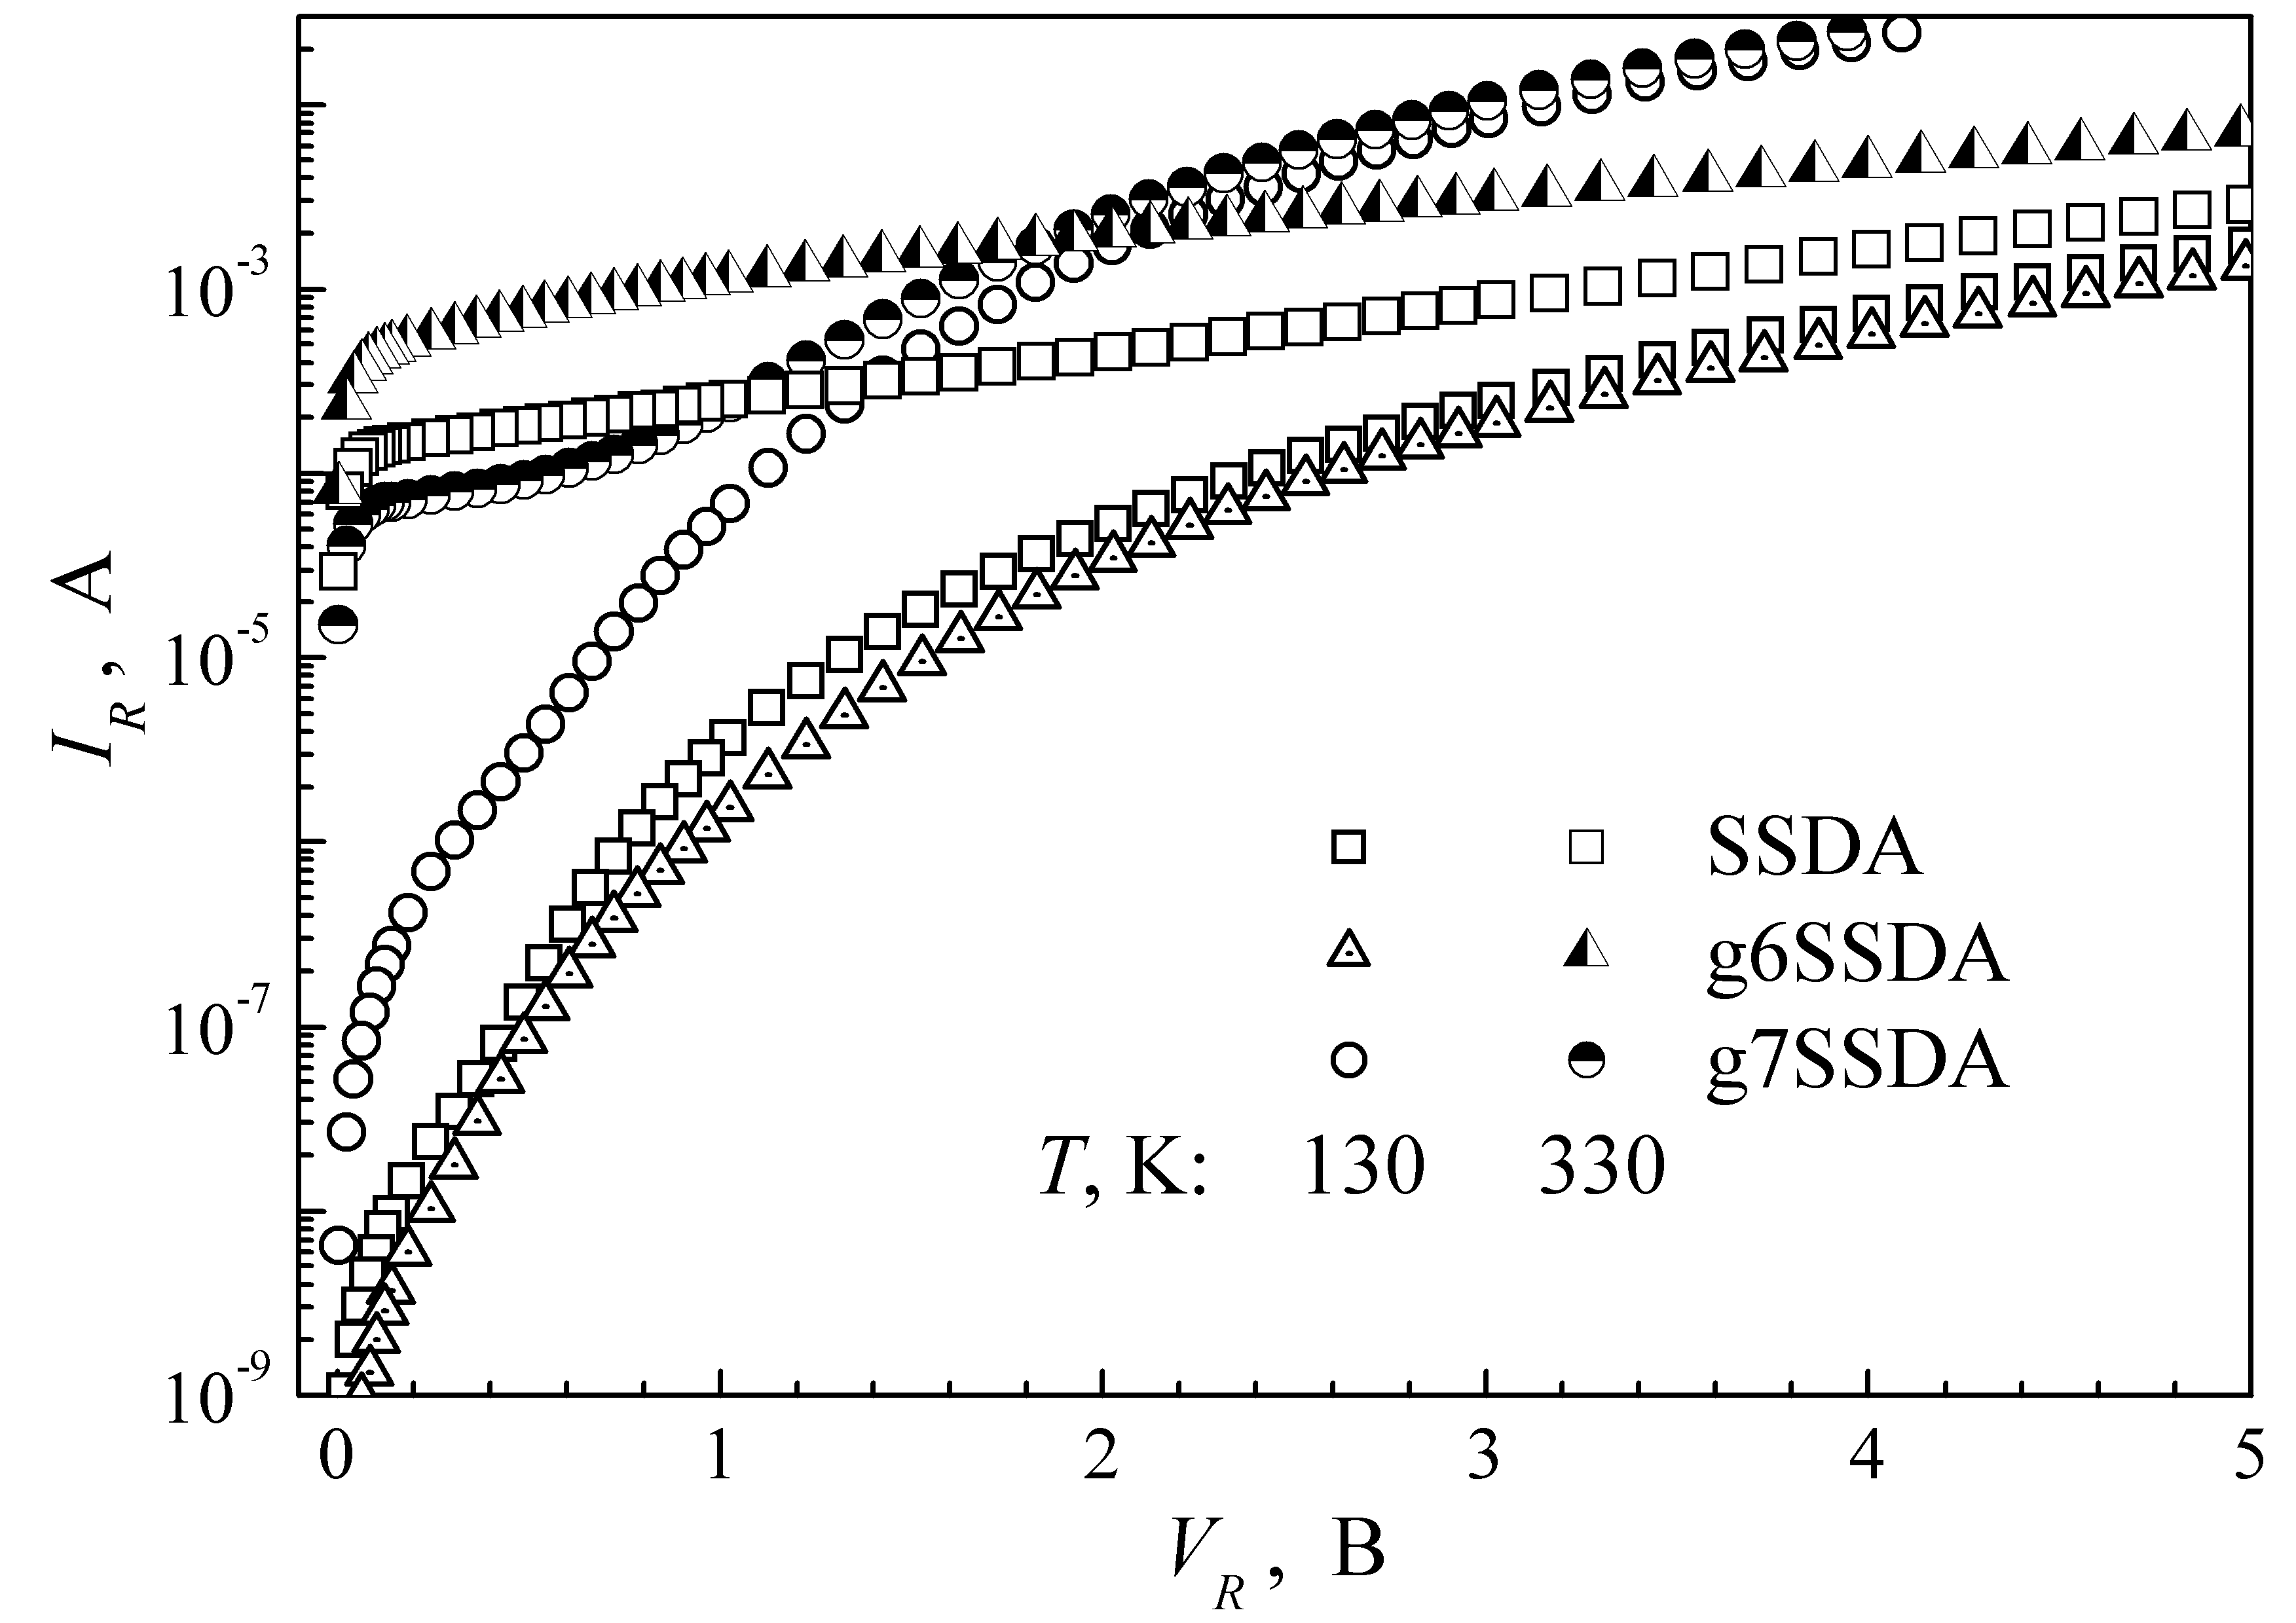
\includegraphics[width=0.8\textwidth]{figIV_SDArRad}
\caption{\label{figIV_SDArRad}
Зворотні характеристики структур SSDA при температурах 130~K (незаповнені точки)
та 330~K (напівзаповнені точки).
$D$, рад: 0 (квадрати), $10^6$ (трикутники), $10^7$ (кола).
}%
\end{figure}

Проведений аналіз показав, що вираз (\ref{eqIr}), який використовувався для опису зворотних гілок ВАХ неопромінених структур,
не може з достатньою точністю відтворити температурну та польову залежності $I_R$ в Al$-n-n^+$--Si---Al після опромінення.
Для апроксимації експериментальних даних був використаний наступний вираз:
\begin{eqnarray}
\label{eqIrRad}
I_R(T,V_R)&=&C_\mathrm{TE}(V_R)T^2\exp\left[-\frac{E_\mathrm{TE}(V_R)}{kT}\right]+I_\mathrm{FN}(V_R)+I_\mathrm{MPT}(T,V_R)\,,
\end{eqnarray}
де
перші два доданки, як і раніше,
пов'язані з ТЕ та температуро--незалежною компонентами зворотного струму,
а третій залежить як від $T$, так і від $V_R$ та описує шлях перенесення заряду, який виник внаслідок опромінення.

Як і для неопромінених структур,
величина $E_{TE}$ залежить від зміщення, проте для g6SSDA та g7SSDA характеристична енергія лінійно залежить від $V_{bb}^{1/4}$
 --- Рис.~\ref{figIrTErad_SDA}.
Тому в цьому випадку вплив неоднорідностей
на термоемісійний зворотній струм менш суттєвий, а зменшення ВБШ пов’язане з дією сил зображення \cite{Rhoderick1988,Andrews}.

Температуро--незалежна компонента $I_\mathrm{FN}$ незалежно від ступеня опромінення має тунельний характер --- див. Рис.~\ref{figIrTErad_SDA},
причому її нахил у координатах Фаулера--Нордгейма однаковий.
Згідно з (\ref{eqFowlNord}) та (\ref{eqFN:Et}) це свідчить про те, що тунелювання відбувається через один і той самий дефектний рівень $E_c-E_t=120$~меВ.
З іншого боку,
зсув залежності $I_\mathrm{FN}/F_m^2=f(F_m^{-1})$ відображає збільшення концентрації відповідних дефектів, яка
особливо помітна для g7SSDA.
Це додатково свідчить, що $I_\mathrm{FN}$ пов'язана з тунелюванням за участю рівнів міжвузольного атому вуглецю С$_i$,
який є вторинним дефектом при опроміненні кремнію $\gamma$--квантами $^{60}$Со \cite{Vavilov1990r}.
Оскільки в наших експериментах температура досягала 330 К, необхідно зауважити, що в роботі \cite{Song1987} показана можливість відпалу С$_i$
 в об’ємному кремнії при температурах 300$\div$350~К шляхом утворення комплексу з міжвузольним атомом кисню чи заміщуючим атомом вуглецю.
Проте, на нашу думку, процеси просторового розділення різнойменно--заряджених дефектів, які можуть відбуватися при $\gamma$--опроміненні бар’єрних структур \cite{Muzafarova}, є причиною стабільності С$_i$ в наших дослідах.
Таким чином, струм $I_\mathrm{FN}$ може бути пов'язаний з прямим  тунелюванням через ГР С$_i$.

\begin{figure}
\center
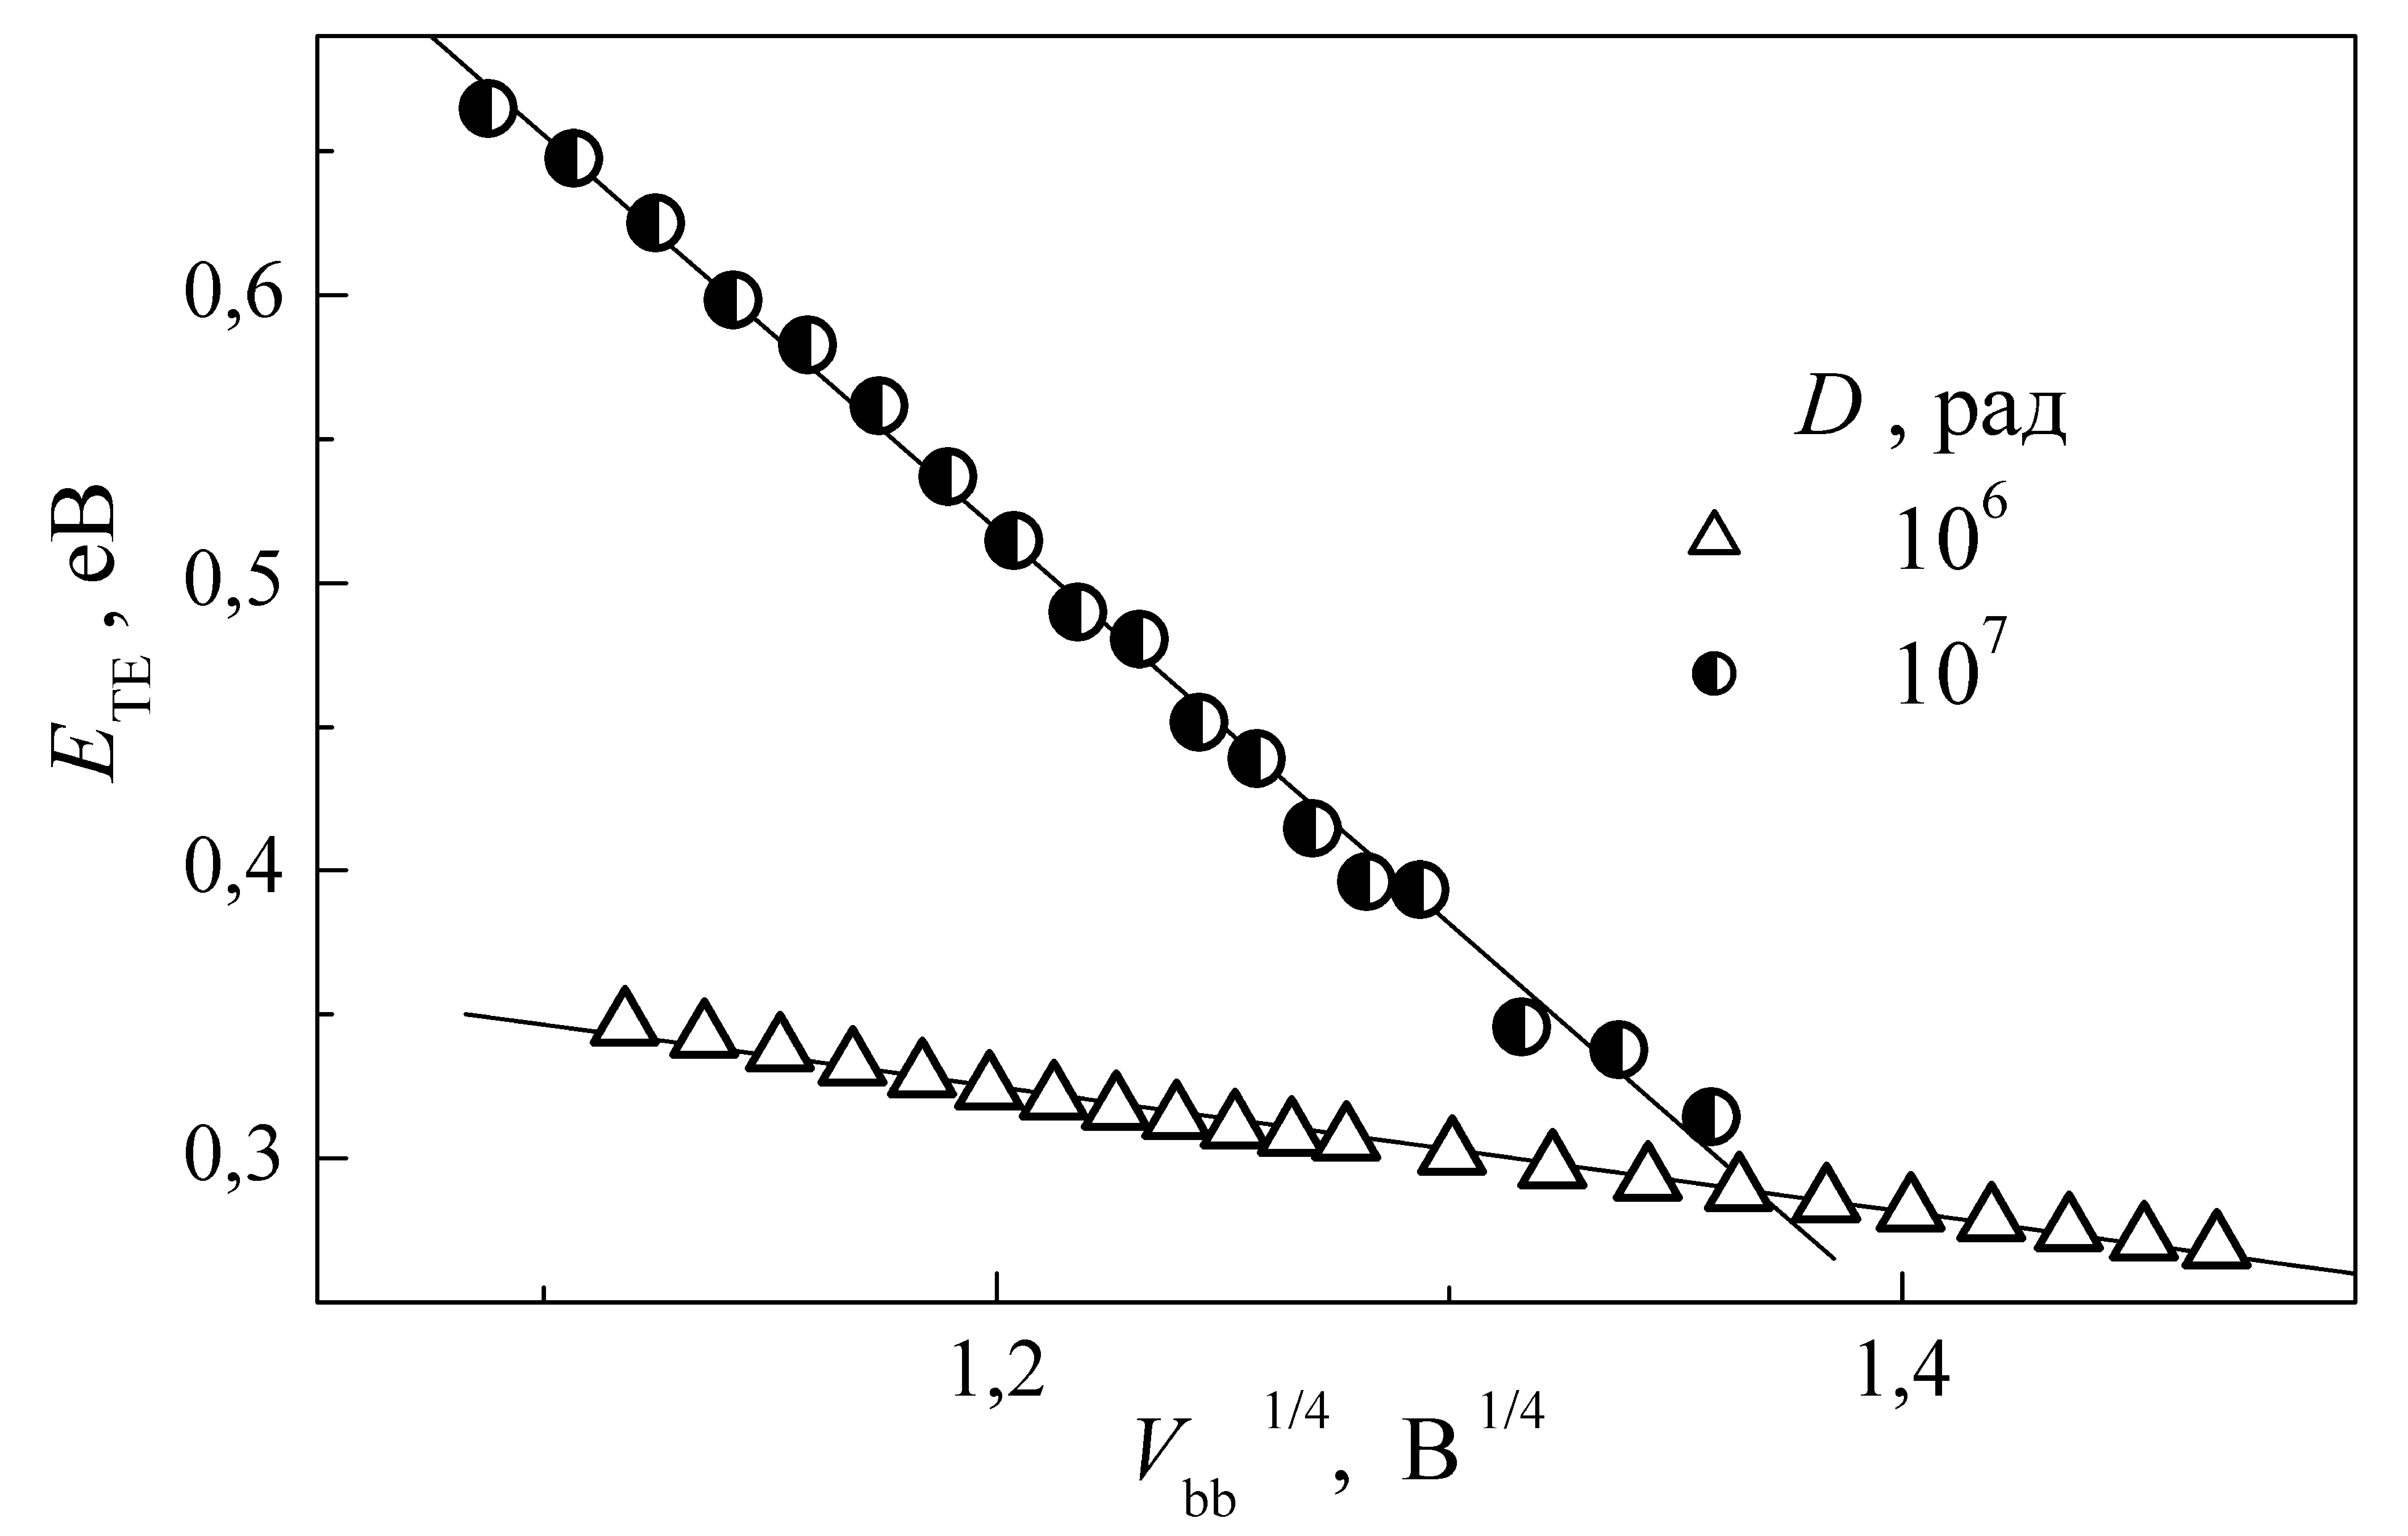
\includegraphics[width=0.65\textwidth]{figIrTErad_SDA}
\caption{\label{figIrTErad_SDA}
Польові залежності характеристичної енергії ТЕ складової зворотного струму структур g6SSDA (трикутники) та g7SSDA (кола).
Точки --- експеримент, прямі --- лінійна апроксимація за методом найменших квадратів.
}%
\end{figure}


\begin{figure}
\center
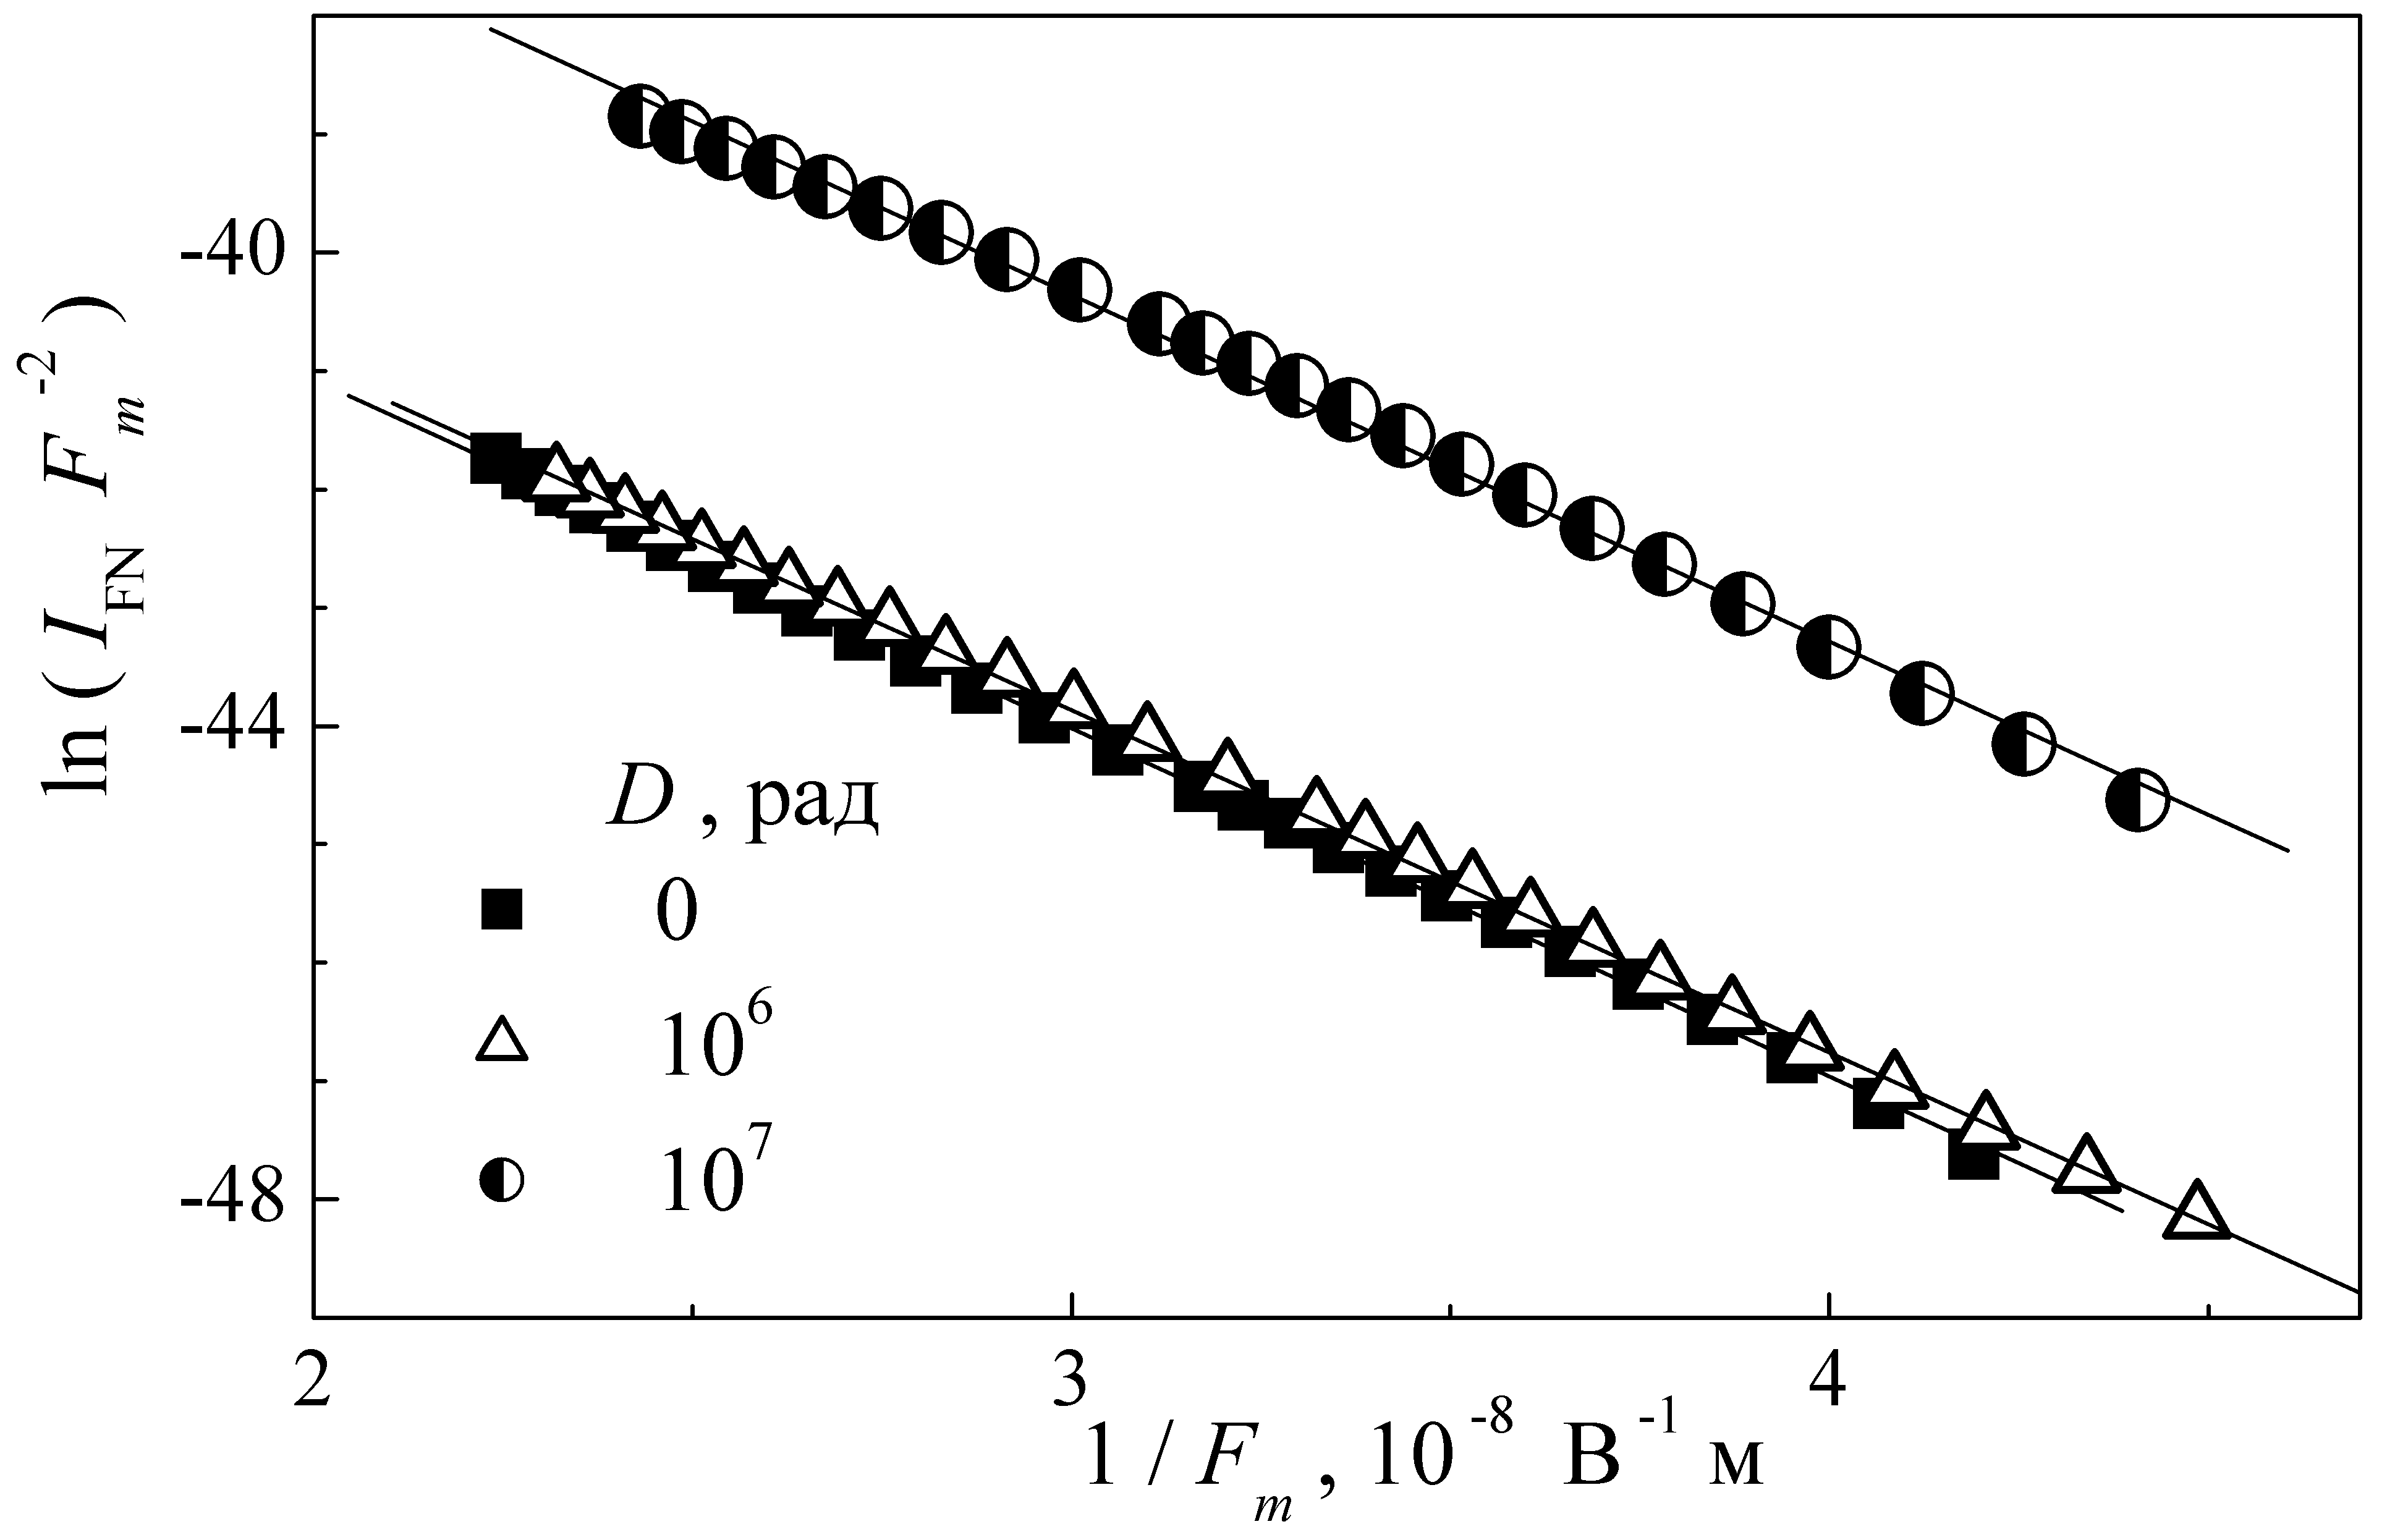
\includegraphics[width=0.65\textwidth]{figIrFNrad_SDA}
\caption{\label{figIrFNrad_SDA}
Залежність температуро--незалежної компоненти зворотного струму
в координатах Фаулера--Нордгейма
структур SSDA (квадрати), g6SSDA (трикутники) та g7SSDA (кола).
Точки --- експеримент, пряма --- лінійна апроксимація за методом найменших квадратів.
}%
\end{figure}


Струм $I_\mathrm{MPT}$, який спостерігається лише в опромінених структурах, зростає з підвищенням поглинутої дози.
Поява нового механізму перенесення заряду після $\gamma$--опромінення є відомим ефектом;
наприклад, згідно з результатами \cite{Gullu:2008,Karatas:2005NIMA}, причинами додаткового струму можуть бути генераційно--рекомбінаційні процеси або
тунелювання.

З літератури \cite{Bulyarskii2001r,Evstropov,Ganichev:2000} відомо, що у структурах МН може протікати струм,
пов’язаний з тунельною багатофононною іонізацією глибоких домішкових центрів.
В цьому випадку для кожної температури існує діапазон полів (загалом тим більший, чим вища температура), коли імовірність багатофононної іонізації $P$
та величина струму експоненційно зростають з підвищенням напруженості електричного поля $F_m$ \cite{Bulyarskii2001r,Ganichev1997,Ganichev:2000}:
$P(F_m,\,T)=P(0,\,T) \exp(F_m^2/F_0^2)$,
де $F_0$ --- деяке характеристичне значення напруженості.
Саме така залежність спостерігається для $I_\mathrm{MPT}$ --- див. Рис.~\ref{figIrPATrad_SDA}.


\begin{figure}
\center
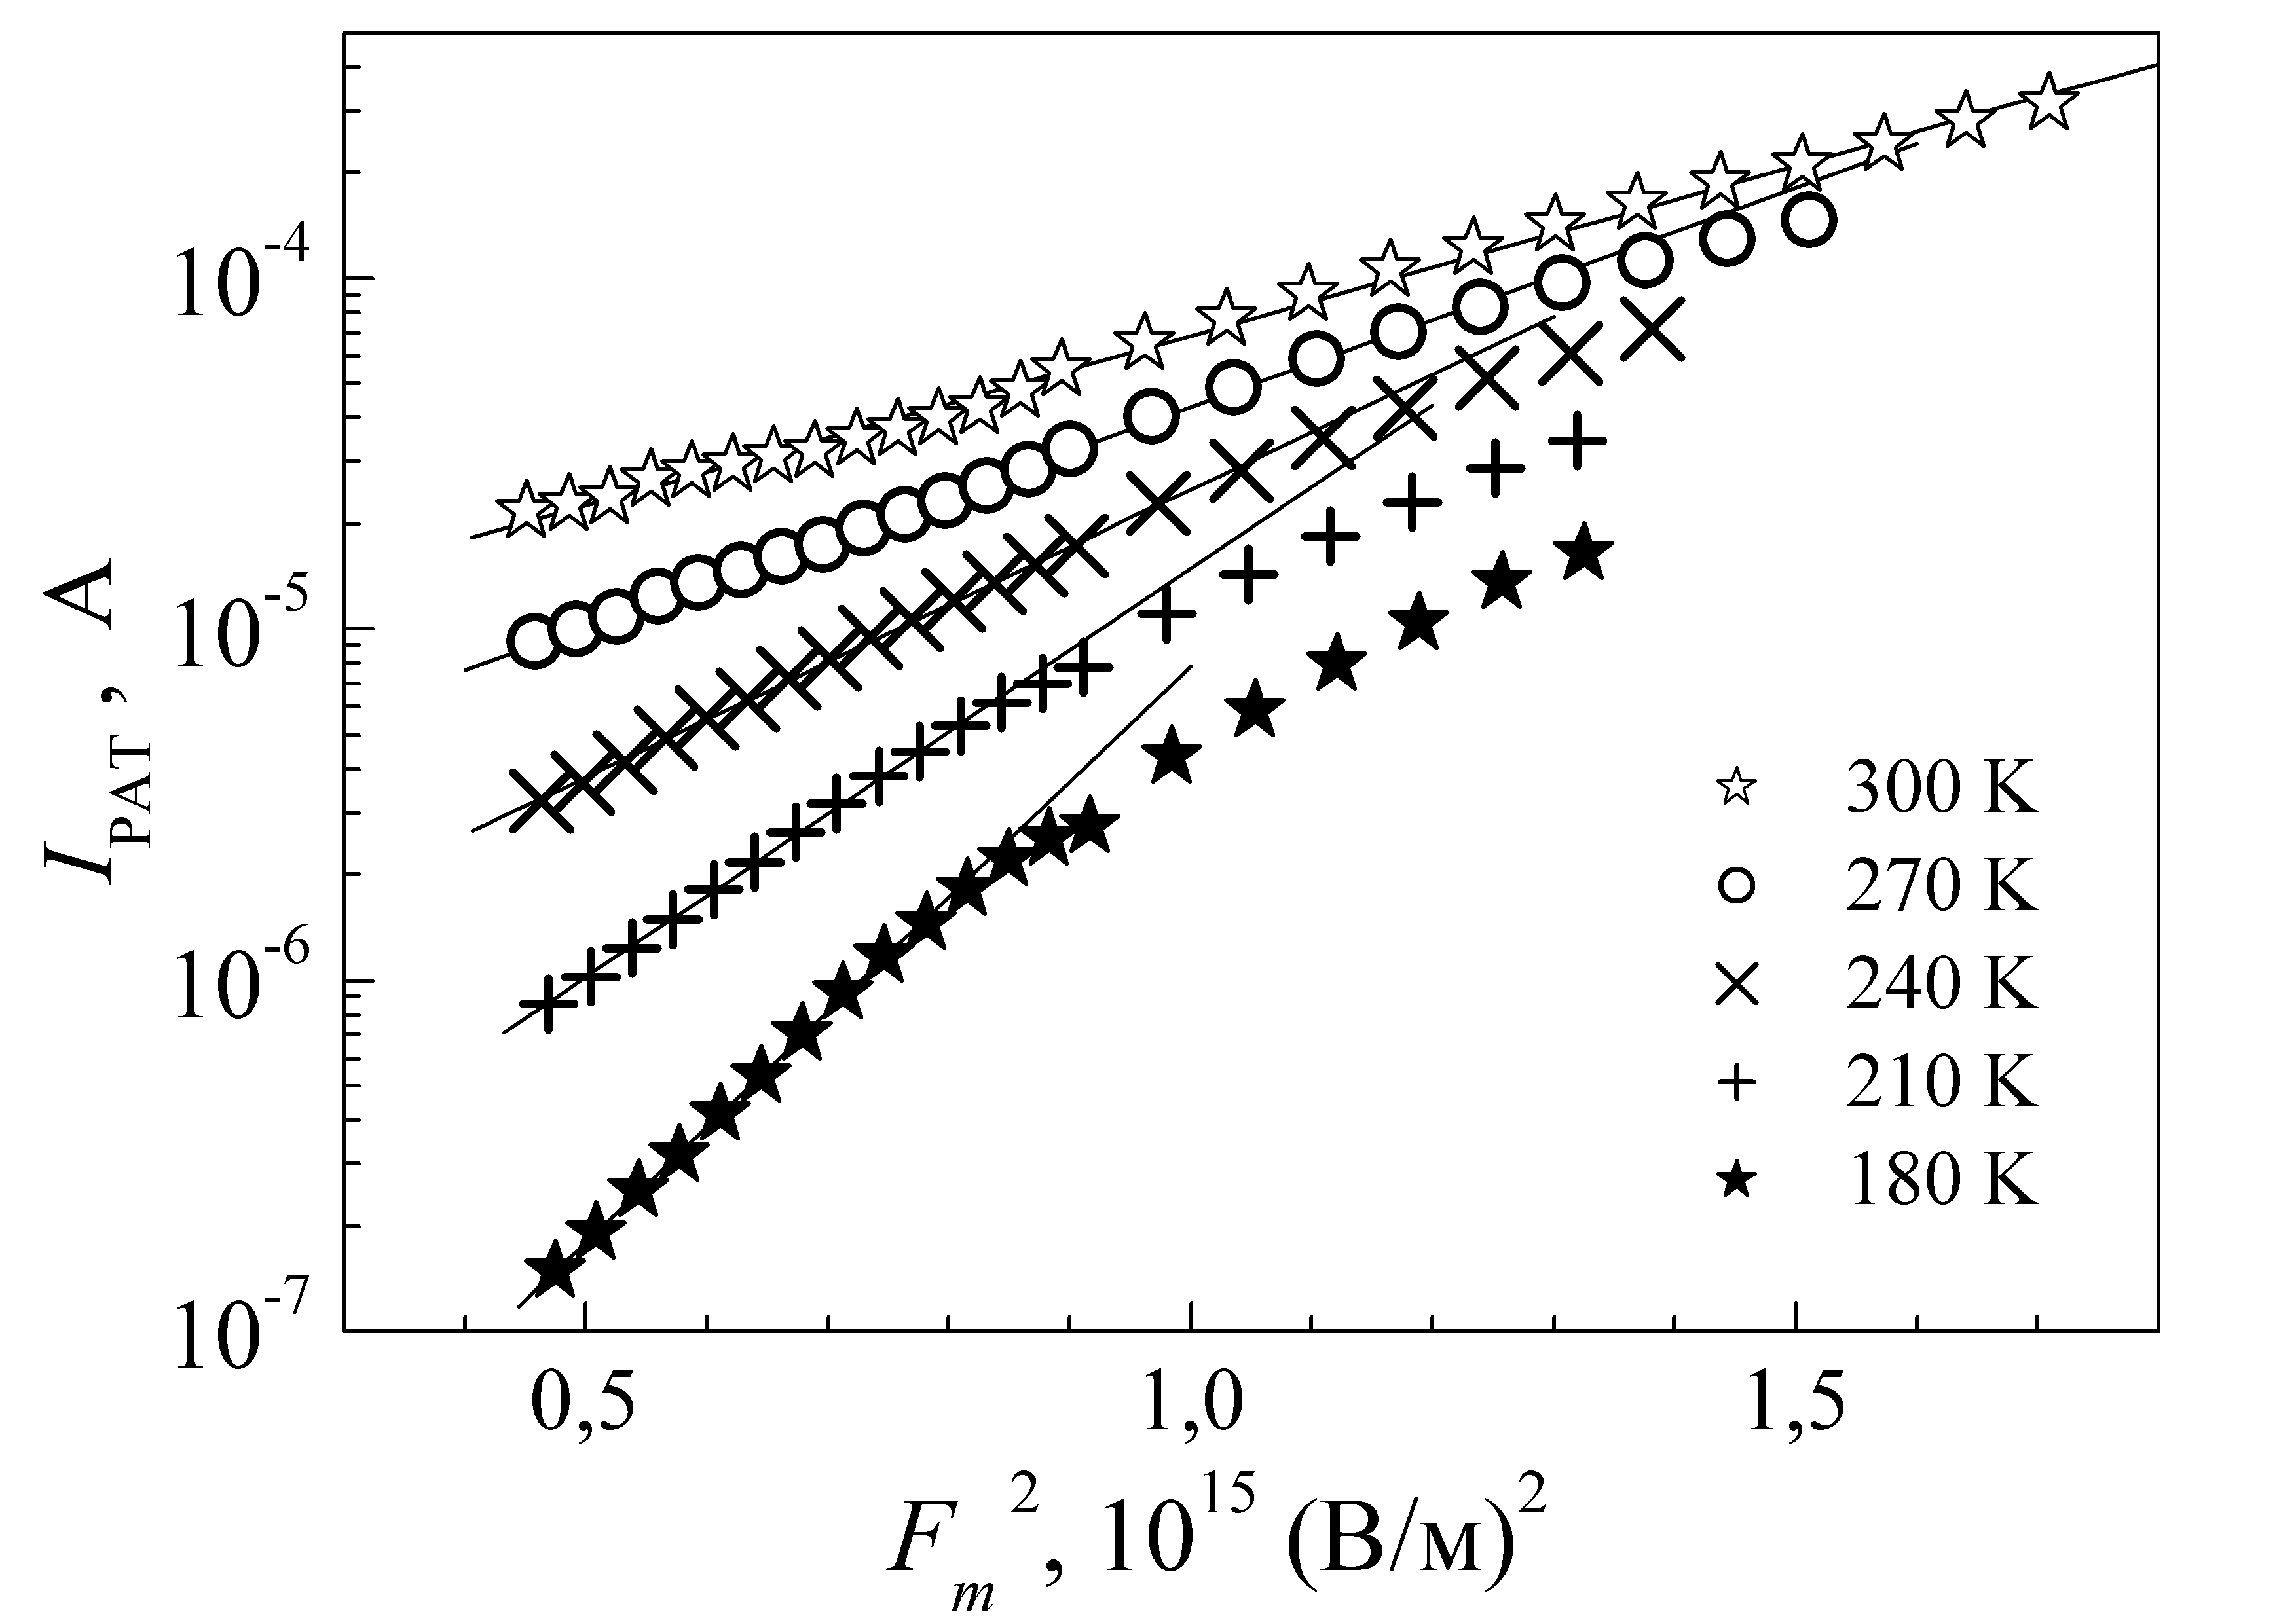
\includegraphics[width=0.65\textwidth]{figIrPATrad_SDA}
\caption{\label{figIrPATrad_SDA}
Польові залежності компоненти зворотного струму $I_\mathrm{MPT}$ при різних температурах для структури g7SSDA.
Точки --- експеримент, пряма --- лінійна апроксимація за методом найменших квадратів.
}%
\end{figure}

Теоретично показано, що коефіцієнт нахилу $F_0$ має залежати від температури, причому \cite{Bulyarskii2001r,Ganichev1997,Ganichev:2000}:
\begin{equation}\label{eqPAT}
    F_0^{\,-2/3}=\left[\frac{d(\ln I_\mathrm{MPT})}{d(F_m^2)}\right]^{1/3}\propto \sqrt[3]{\frac{q^2\hbar^2}{24k^3m^*}}\,\frac{1}{T}\,.
\end{equation}

Нахил залежності $\ln I_\mathrm{MPT}\sim F^2$ дійсно є лінійною функцією оберненої температури (Рис.~\ref{figIrPATF0rad_SDA}).
Значення, отримані шляхом лінійної апроксимації даних на Рис.~\ref{figIrPATF0rad_SDA}
($2,9\cdot10^{-3}$ та $0,6\cdot10^{-3}$~K$\cdot$м$^{2/3}$$\cdot$В$^{-2/3}$ для g6SSDA та g7SSDA, відповідно)
цілком задовільно узгоджуються з теоретичним значенням
$q^2\hbar^2/(24k^3m^*)=1,7\cdot10^{-3}$~K$\cdot$м$^{2/3}$$\cdot$В$^{-2/3}$.
Тобто, причиною виникнення ще однієї складової зворотного струму є поява радіаційних дефектів та пов’язаних з ними рівнів у забороненій зоні,
за участю яких і відбуваються процеси багатофононної іонізації в області просторового заряду.



\begin{figure}
\center
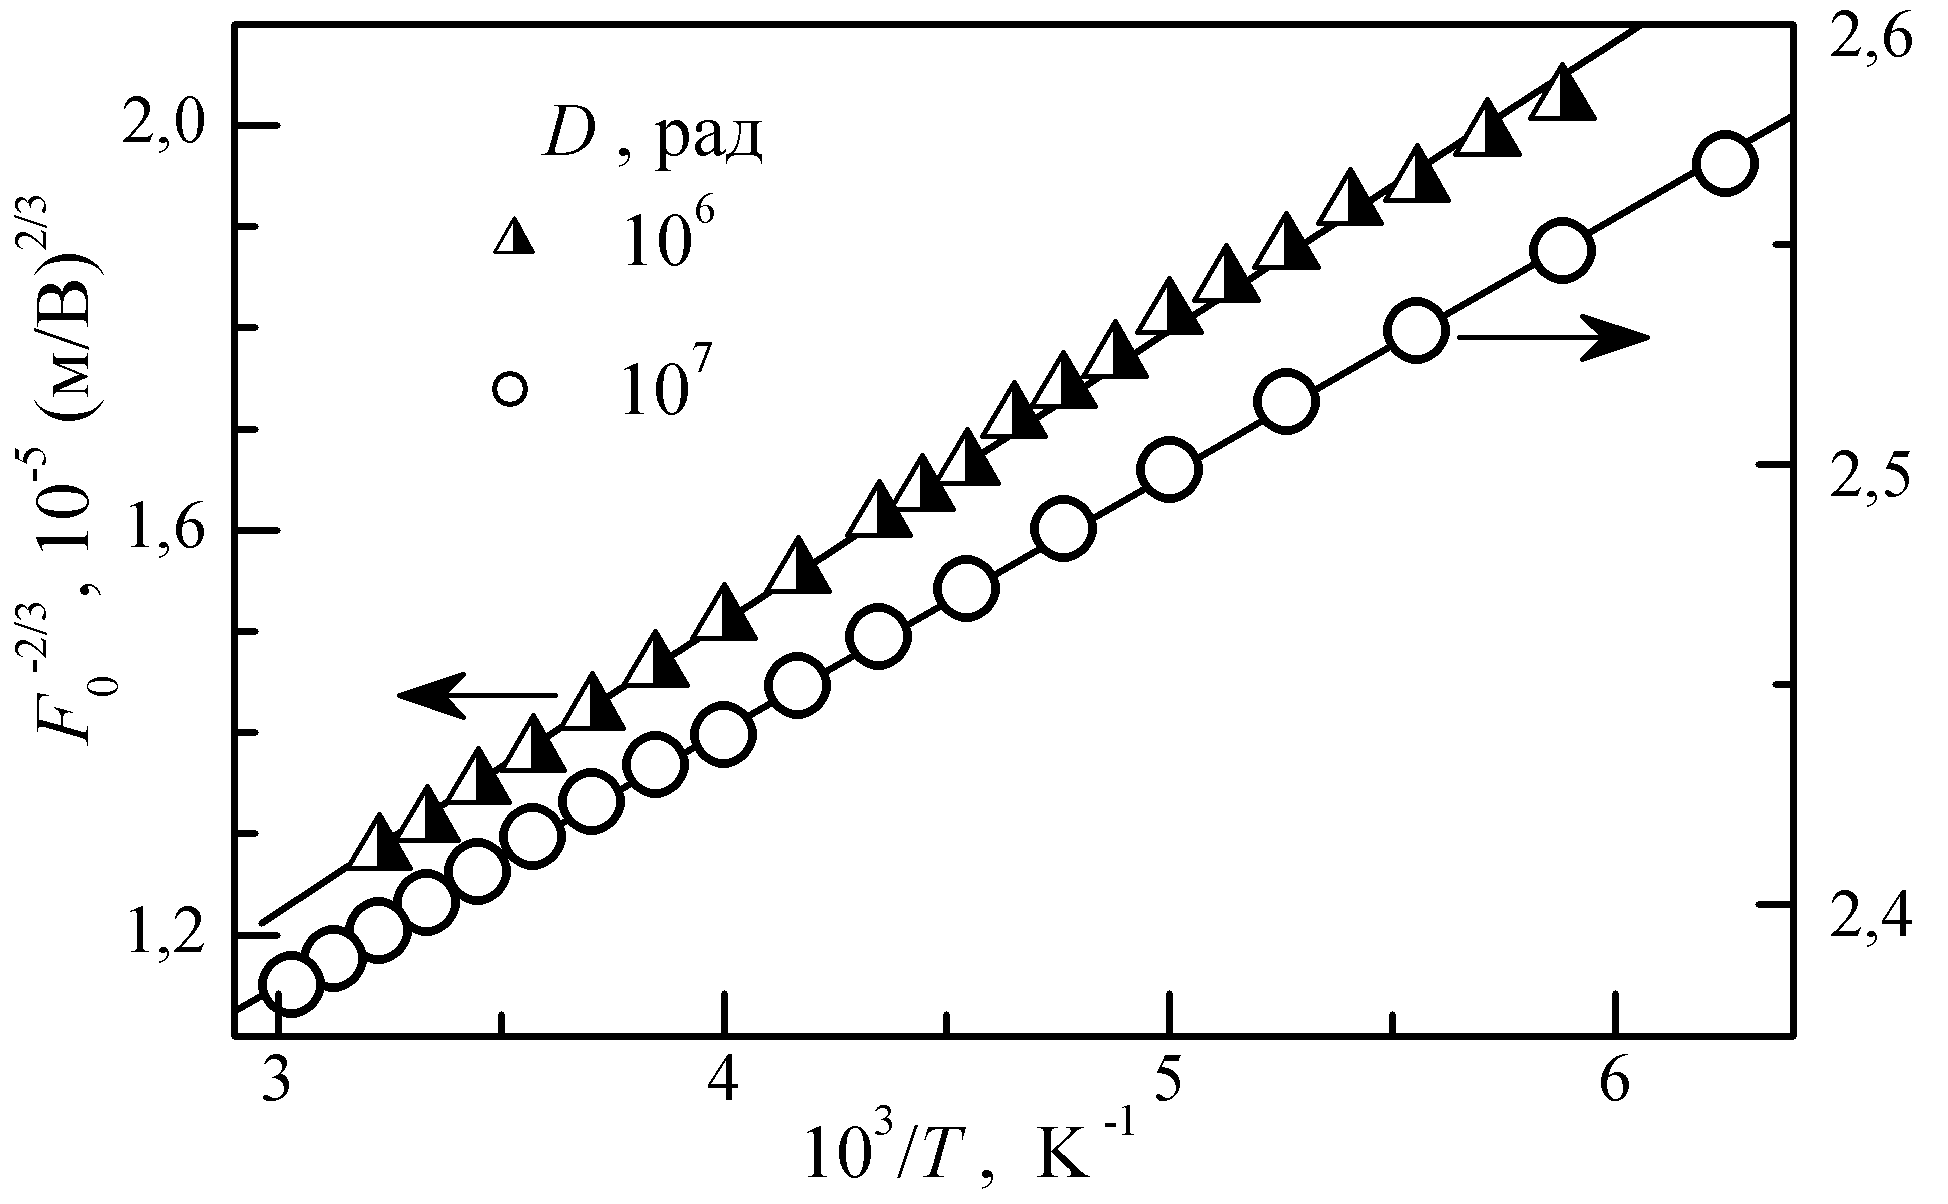
\includegraphics[width=0.65\textwidth]{figIrPATF0rad_SDA}
\caption{\label{figIrPATF0rad_SDA}
Температурна залежність коефіцієнту нахилу польової залежності компоненти зворотного струму $I_\mathrm{MPT}$.
Точки – експеримент, лінії – лінійна апроксимація за методом найменших квадратів.
}%
\end{figure}

На Рис.~\ref{figeIrRad_SDA} показані температурні залежності відносних внесків $\nu_\mathrm{TE}$, $\nu_\mathrm{FN}$ та $\nu_\mathrm{MPT}$
кожної з компонент у загальний зворотний струм, розраховані аналогічно до виразів, наведених на с.~\pageref{nu_IR} при певних значеннях $V_R$.
Видно, що
\begin{enumerate}[label=\asbuk*),leftmargin=0em,itemindent=1.5em]
\item струм $I_\mathrm{FN}$ є основним при низьких температурах, його внесок зменшується при зростанні $T$ і є найбільшим для g7SSDA;
\item в g6SSDA тунельний струм перевищує ТЕ складову при $T<250$~K, що співпадає з результатами, отриманими при аналізі прямого струму;
\item в g7SSDA внесок $I_\mathrm{TE}$ стає переважаючим лише при $T>300$~K, тоді як при нижчих температурах домінюючою є температуро--незалежна компонента.
\end{enumerate}

\begin{figure}
\center
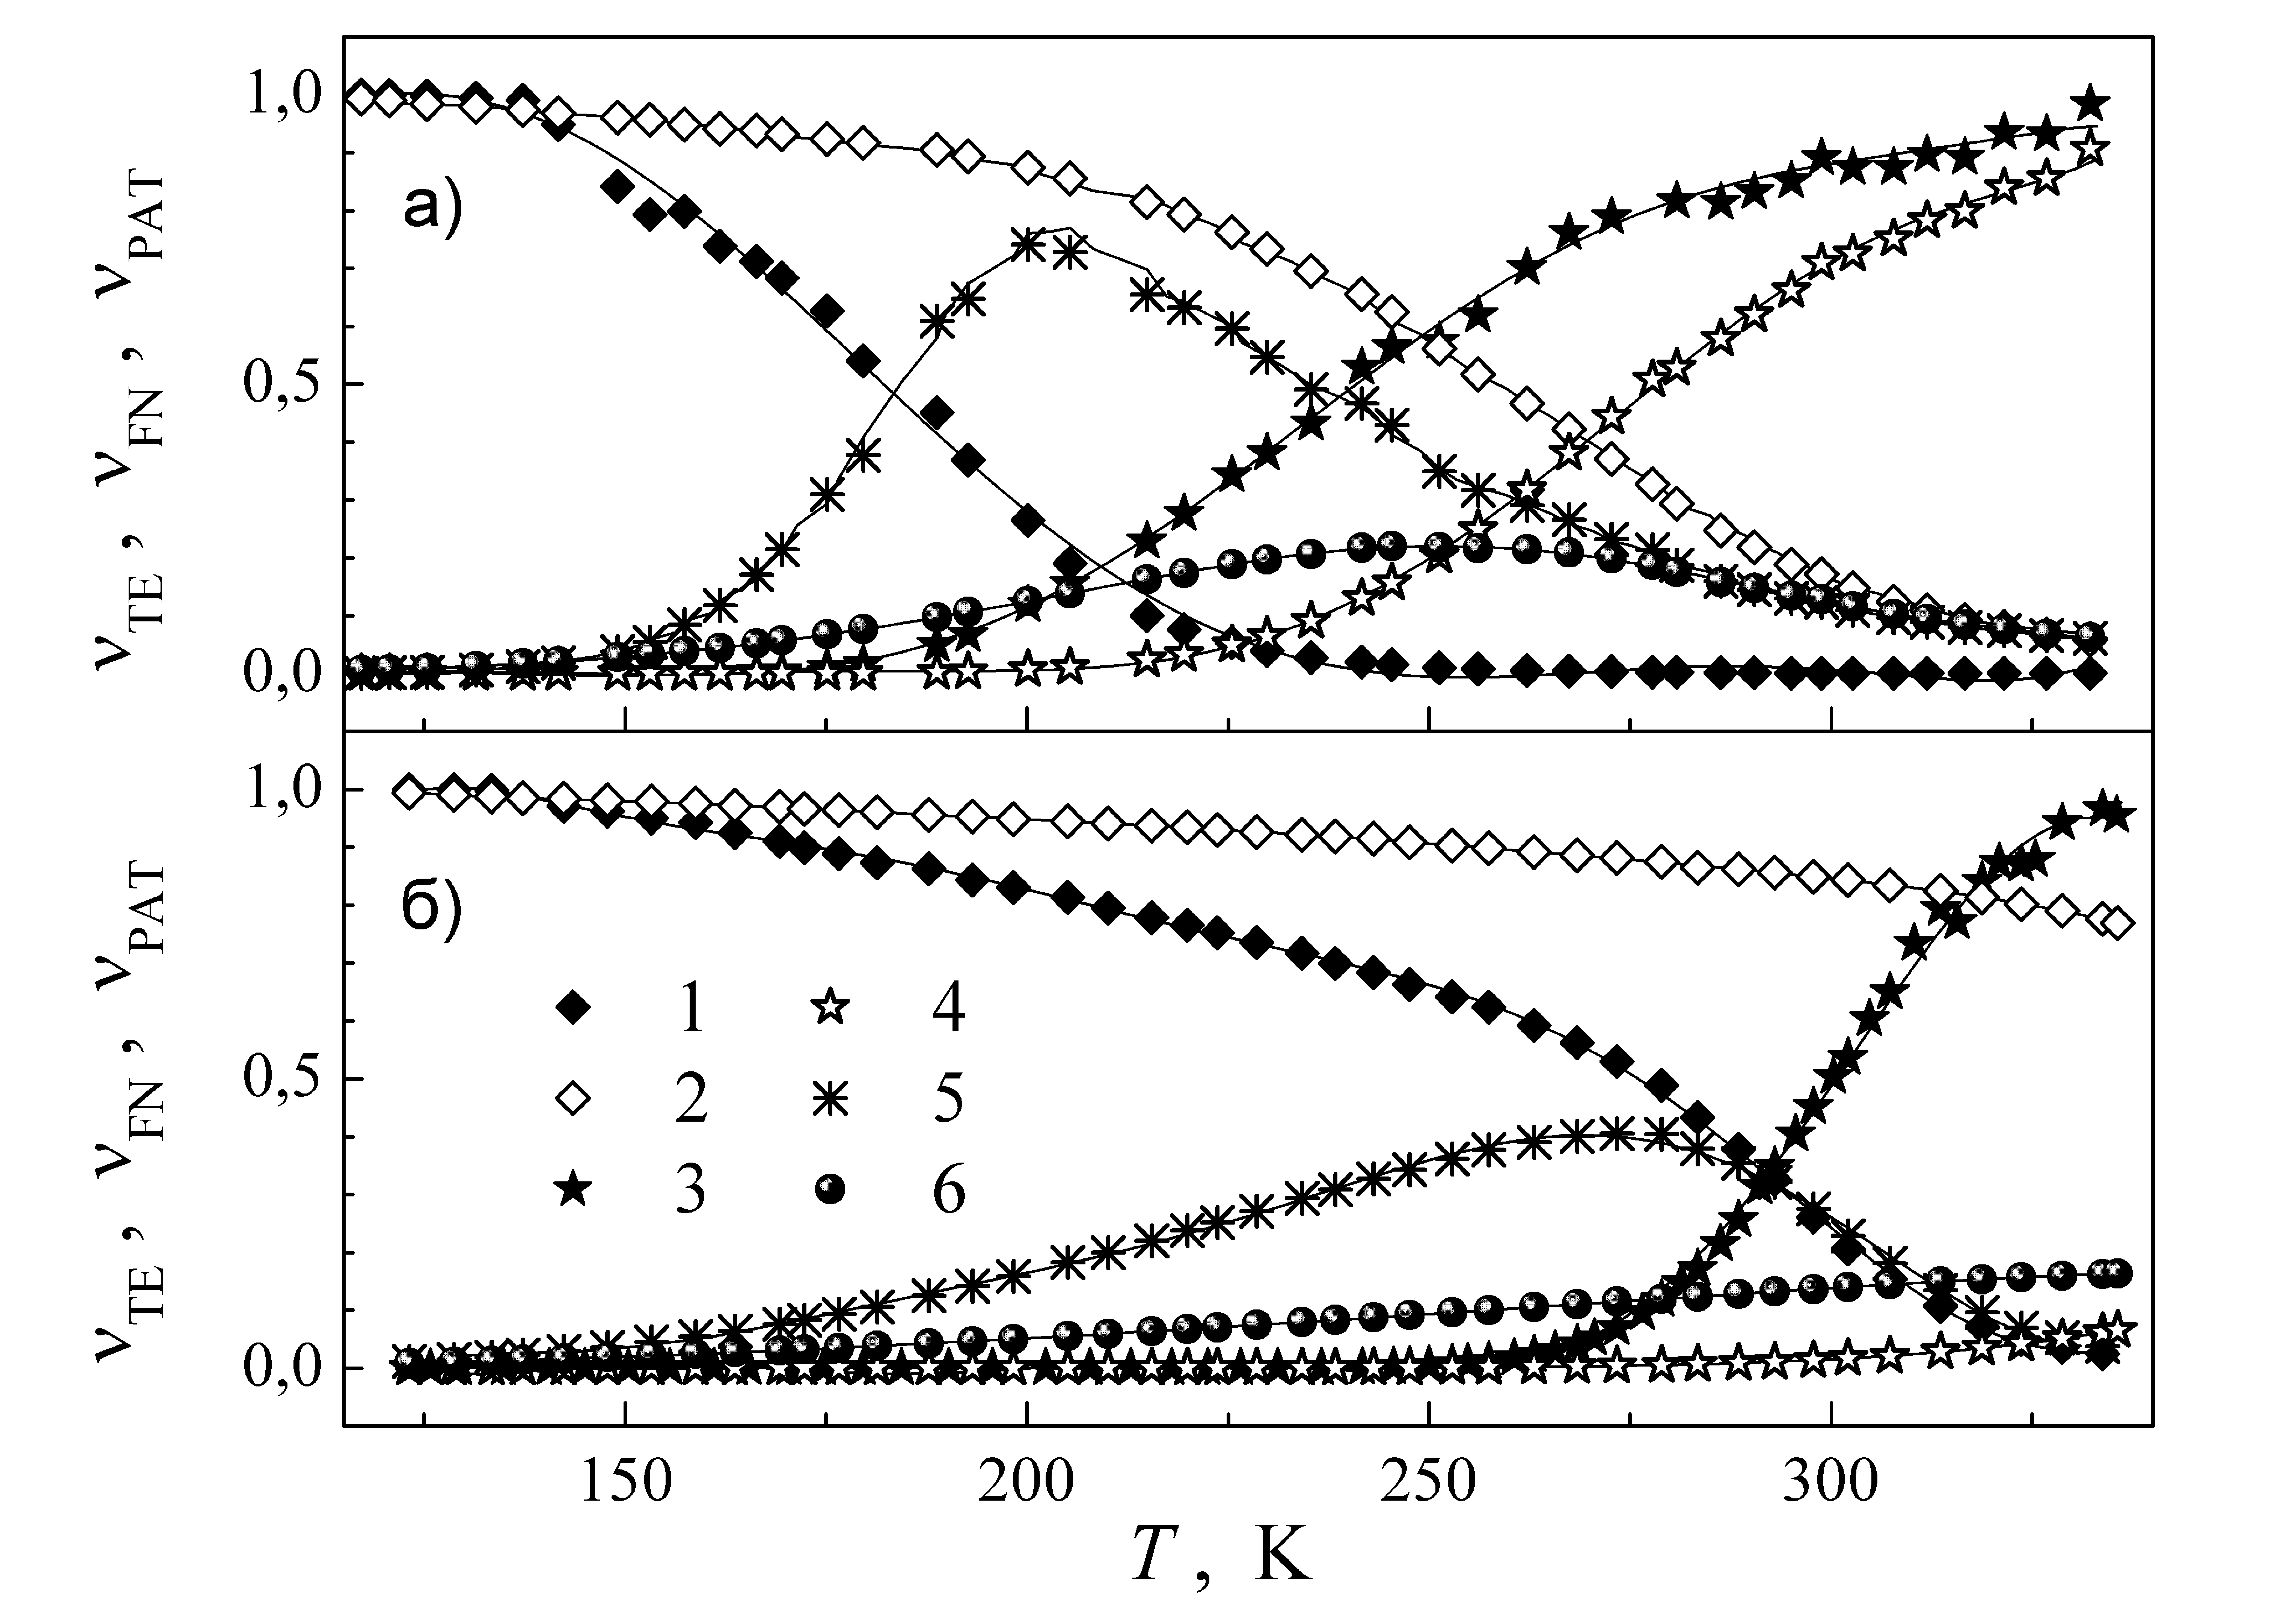
\includegraphics[width=0.8\textwidth]{figeIrRad_SDA}
\caption{\label{figeIrRad_SDA}
Температурні залежності відносних внесків у зворотний струм
структур g6SSDA (a) та g7SSDA (б)
при $V_R=0,5$~В та $V_R=3$~В.
}%
\end{figure}

Зазначимо, що останній факт разом зі слабкою температурною залежністю струму насичення ВТКС g7SSDA при $T=150\div220$~K (Рис.~\ref{figIsTrad_SDA},а, крива 2)
доводить, що в цьому температурному діапазоні тунелювання є основним механізмом перенесення заряду і при прямому зміщенні.
Відомо \cite{Yu}, що наявність тунельної компоненти є причиною помилок у визначенні $A^*$ та ВБШ за допомогою залежності Річардсона.
На нашу думку, вплив тунелювання залишається достатньо суттєвим для g7SSDA і в інтервалі температур 260$\div$330~K і саме це є причиною
відмінності отриманого значення сталої Річардсона (Таблиця~\ref{tabSDAParRad}) та відомого з літератури, а також перевищення $\Phi_b^0$ величини $\Phi_{b,CV}$.

Узагальнюючи картину змін параметрів структур Al$-n-n^+$--Si---Al внаслідок опромінення $\gamma$--квантами $^{60}$Co зауважимо наступне.
До опромінення перенесення заряду при прямому зміщенні у всьому дослідженому інтервалі температур відбувалося внаслідок ТЕ через неоднорідний бар'єр,
причому при $T>230$~K середня висота бар'єру $\Phi_b^0=0,663$~В, а стандартне відхилення $\sigma_{\Phi0}=0,04$~В.
Після того, як поглинута доза досягла $10^6$~рад, домінуючим механізмом перенесення заряду в діапазоні температур
$120\div240$~K як при прямому зміщенні, так і при зворотному стає DAT з характеристичною енергією $E_{00}=17,8$~меВ.
Це пов'язано з появою у збідненому прошарку РД, зокрема міжвузольних атомів вуглецю, які спричинюють збільшення
концентрації рівнів у забороненій зоні, і, отже, інтенсифікує процеси тунелювання, у тому числі і багатофононного.
При $T>260$~K основним механізмом залишається термоелектронна емісія через неоднорідний бар'єр, проте значення $\Phi$ та $\sigma_{\Phi0}$
зростають до 0,772~В та 0,1~В, відповідно.
Аналіз НТКС показав, що поява додаткового струму, як і для неопромінених структур, пов'язана з ефективним проходженням носіїв через області зниженого бар'єру,
причому загальна площа патчів не змінилась, проте зросла висота бар'єру (з 54 до 74~мВ).
Тобто, відбуваються радіаційно--індуковані процеси зміни як характеристик області поза межами патчів, так і самих неоднорідностей.
Причиною зміни середнього значення ВБШ та $\Phi_{b,p}$ може бути накопичення на інтерфейсній границі структур МН
РД акцепторного типу.
Зауважимо, що ефекти просторового розділення точкових дефектів з протилежним зарядом, індукованих $\gamma$--опроміненням, внаслідок дії пружних полів
у бар'єрних структурах достатньо широко відомі в літературі \cite{Shcherb, Muzafarova}.
Щодо збільшення $\sigma_{\Phi0}$, то зазначимо, що можливою причиною появи патчів вважаються, зокрема, дислокації \cite{GELCZUK2014}.
У приповерхневих шарах Si структур Al$-n-n^+$--Si---Al, ідентичних за будовою до досліджених, виявлено скупчення дислокацій та дефекти пакування \cite{VOROBETS2005,Vorobets},
що є додатковим аргументом на користь того, що причиною появи областей неоднорідності ВБШ є самі ці протяжні дефекти.
З іншого боку відомо, що утворені в процесі опроміненні вільні носії можуть захоплюватись на дефекти пакування та бути причиною
полегшення руху дислокацій --- відоме явище так званого радіаційно--підсиленого дислокаційного ковзання (REDG, radiation--enhanced dislocation glide) \cite{REDG}.
Тобто, в нашому випадку $\gamma$--опромінення викликає переміщення протяжних дефектів та їх часткове перегрупування з утворенням більших за розміром
скупчень.
Ефекти зменшення загальної кількості таких дефектів внаслідок фотонного (лазерного) опромінення спостерігалося і раніше в роботах \cite{VOROBETS2005,Vorobets}.
В рамках моделі неоднорідного контакту (див. формули (\ref{eqGigFSigG}) та (\ref{eqGammaP})), збільшення розкиду розмірів патчів має спричинити зростання $\sigma_{\Phi0}$.
Збільшення впливу патчів маскує зростання ВБШ за їх межами і викликає ефективне зменшення висоти бар'єру, яка визначається безпосередньо з ВАХ.

При збільшенні дози до $10^7$~рад концентрація РД суттєво зростає --- див., наприклад Таблицю~\ref{tabDefectNt}, де представлені результати оцінки дефектоутворення
у кристалах кремнію при таких же дозах процеси $\gamma$--опроміненням, які використовувалися для модифікації
структур SSDA.
Відомо \cite{Boltovets}, що в ДШ релаксація механічних напруг може відбуватися внаслідок гетерування ТД.
На нашу думку, в досліджених структурах такими центрами гетерування є саме патчі.
В результаті накопичення ними від'ємно заряджених дефектів (як радіаційних, так і тих, що були наявні в кристалі до опромінення, але внаслідок іонізації
стали більш рухливими) характер перенесення заряду через ці області змінився з термоемісійного на тунельний.
Тобто, патчі почали виконувати роль тунельних шунтів і перестали впливати на ТЕ процеси.
Як наслідок,
а)~НТКС при прямому зміщенні суттєво зросла, причому перенесення заряду почало відбуватися завдяки процесам DAT з $E_{00}=80$~меВ;
б)~тунельний струм став переважаючим не лише при зворотному зміщенні практично у всьому дослідженому температурному інтервалі,
але й при прямому зміщенні при $T=150\div220$~K;
в)~прямий струм при $T=260\div330$~K, в основному, визначається ТЕ процесами через бар'єр висотою близько 710~мВ,
проте вплив тунелювання у цьому температурному діапазоні не може бути знехтуваний;
г)~ефективна ВБШ, яка визначається безпосередньо з ВАХ, збільшилась порівняно з  $D=10^6$~рад, на противагу реальному зменшенню висоти бар'єру в однорідній області внаслідок гетерування дефектів акцепторного типу.

Необхідно зауважити, що зі збільшенням поглинутої дози $\gamma$--квантів $^{60}$Co спостерігалися ефекти як немонотонної зміни механічних напруг
в епітаксійних плівках, так і зміни заряду радіаційних дефектів, накопичених на границі розділу \cite{Muzafarova, Belyaev}.
Ці явища також є непрямим доказом на користь запропонованого механізму радіаційно--індукованої перебудови кремнієвих діодів Шотки.



\section{Вплив ультразвукового навантаження на перенесення заряду в $\gamma$--опромінених та неопромінених структурах Al$-n-n^+$--Si---Al\label{MSSi_USL}}

\subsection{Режими ультразвукового навантаження структур Al$-n-n^+$--Si---Al}

Схема акустичного навантаження структур Al$-n-n^+$--Si---Al наведено на Рис.~\ref{figUSL:SDA}.
Відмінність від схеми, зображеної на Рис.~\ref{figUSL:SC}, полягає у наявності діелектричного прошарку,
необхідного для електричної розв'язки при вимірюванні ВАХ.
Для оцінки параметрів ультразвукового навантаження використовувалися формули (\labelcref{eqAmpUS,eqWus,eqM0,eqDefUS}) та дані Таблиці~\ref{tabLNO}.

\begin{figure}[b]
\center
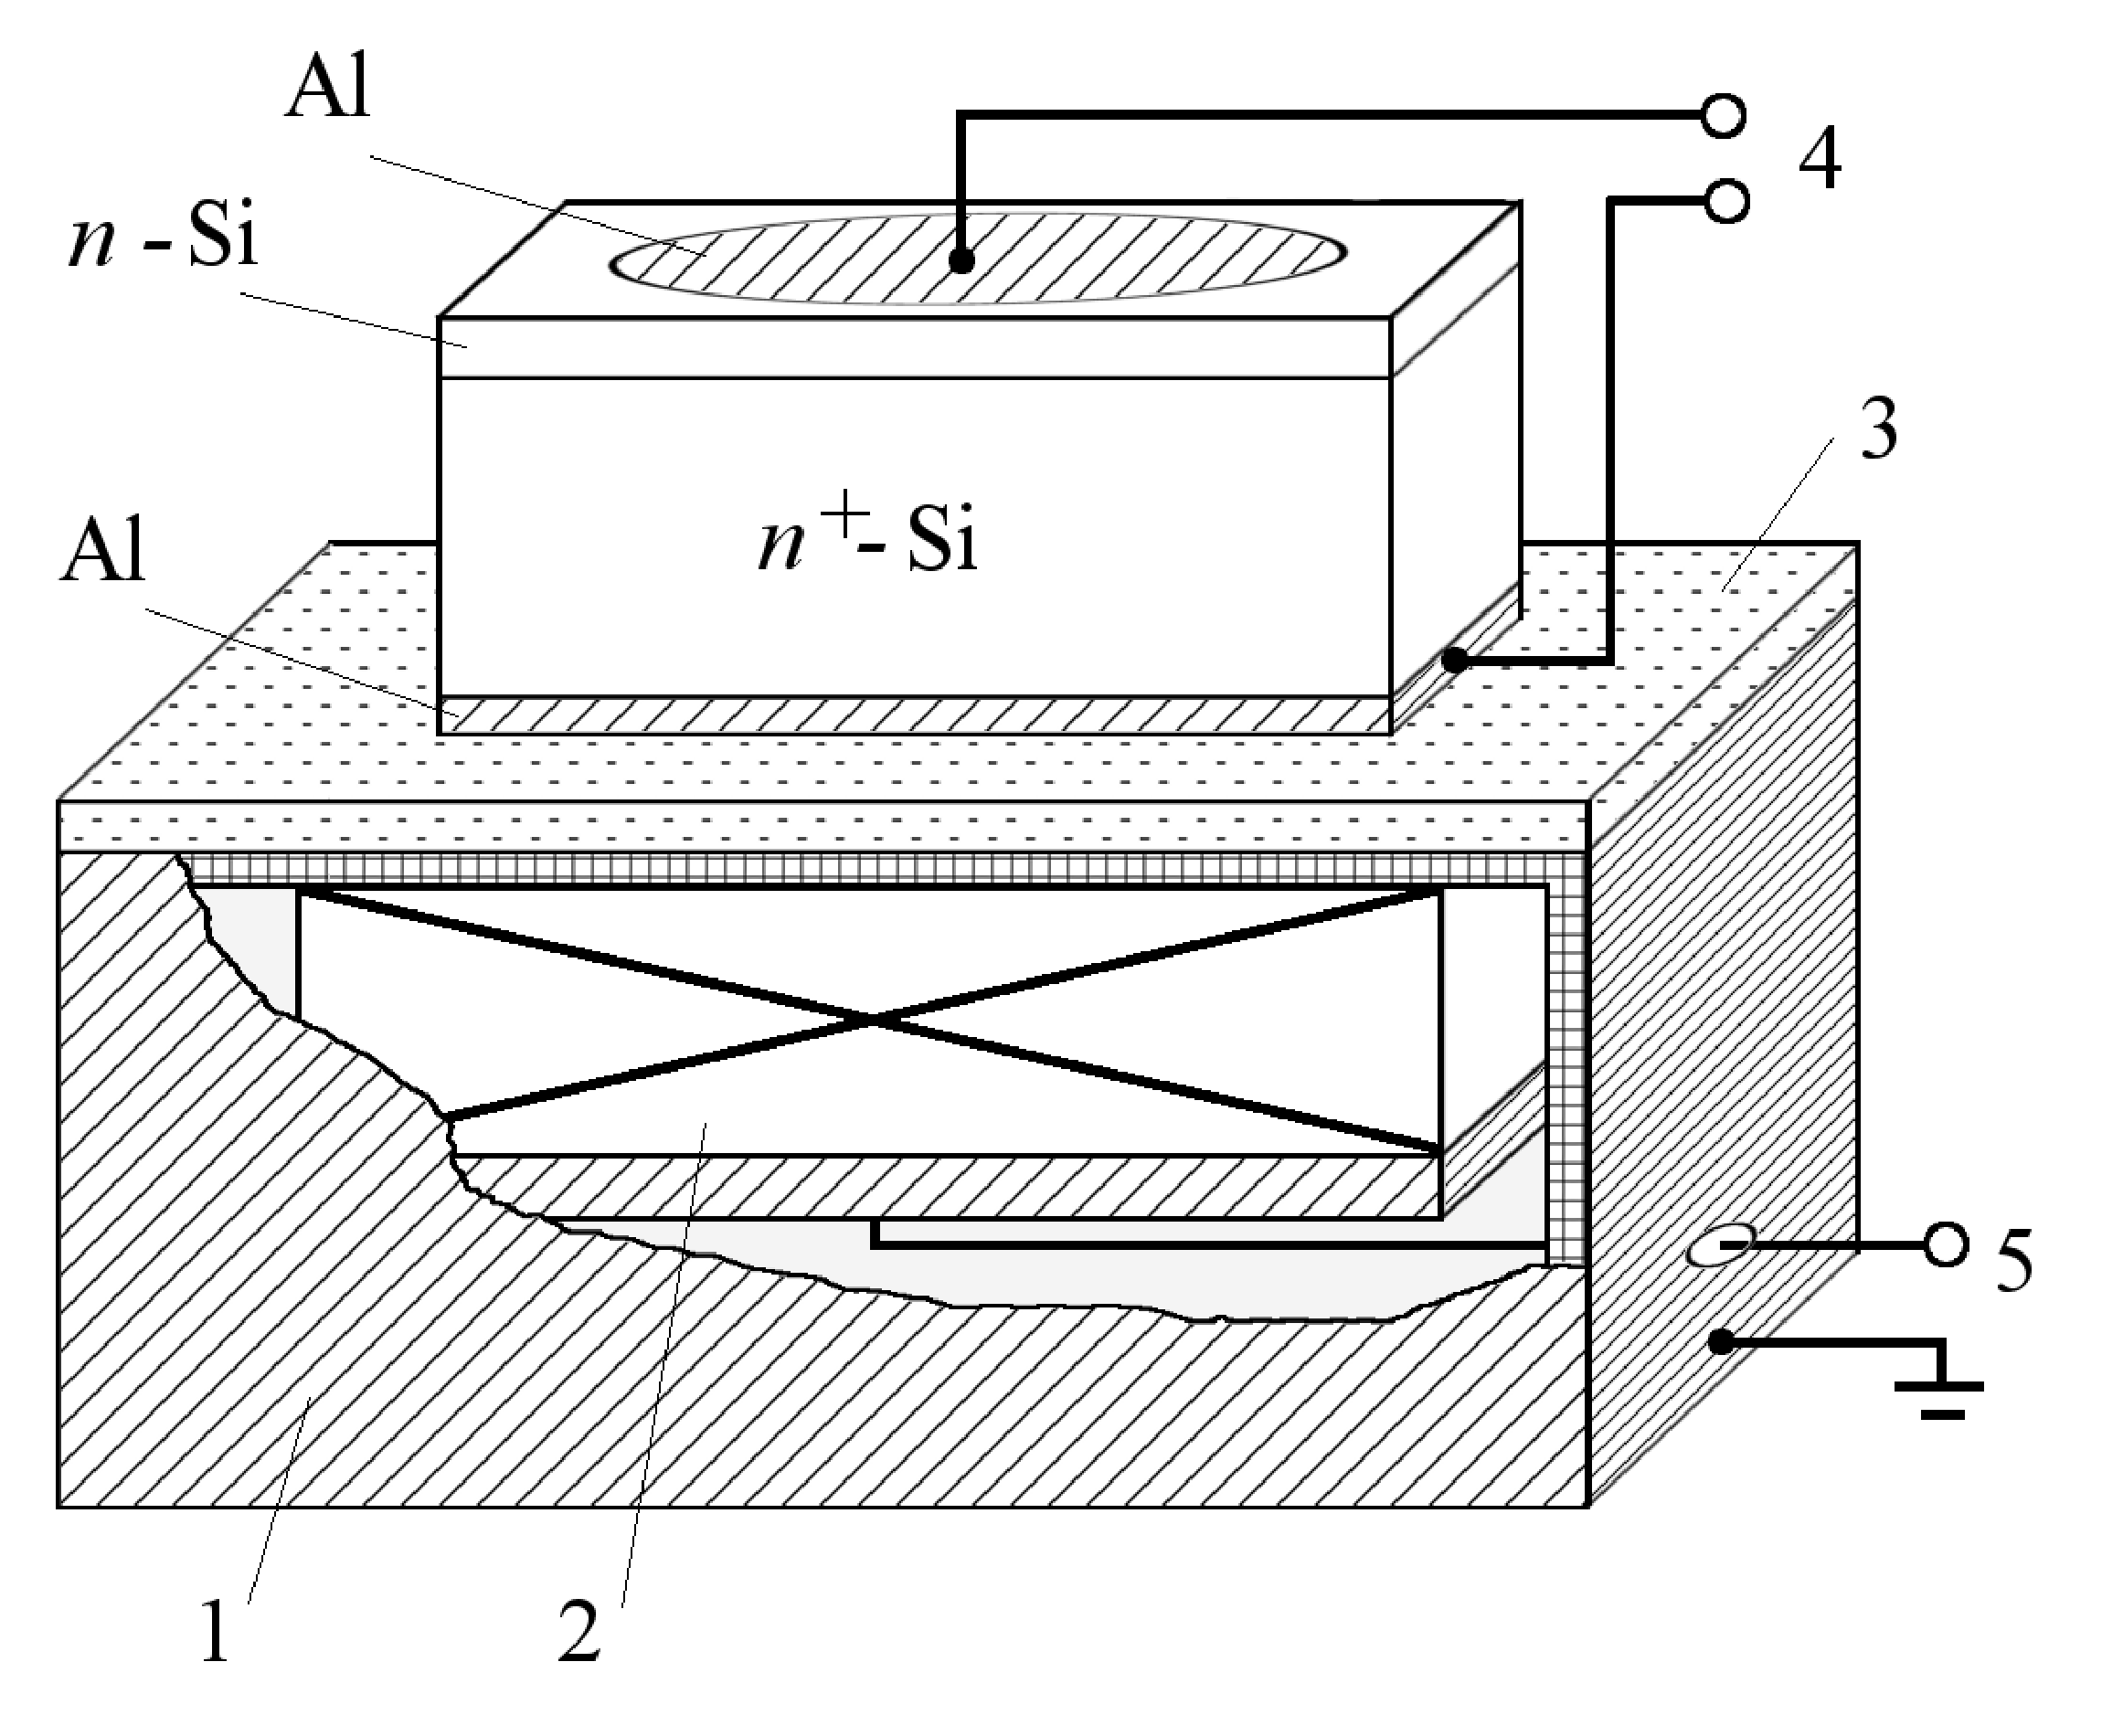
\includegraphics[width=0.6\textwidth]{USL_SDA}%
\caption{\label{figUSL:SDA}
Використані схеми УЗН.
1 --  екран (алюмінієва фольга, товщина 0,012 мм);
2 --- п'єзоелектричний перетворювач (LiNbO$_3$);
3 --- діелектричний прошарок (слюда, товщина 0,03 мм);
4 --- контакти для вимірювання ВАХ;
5 --- контакти для збудження УЗ.
}
\end{figure}



При досліджені АІ ефектів в зразках збуджувалися повздовжні хвилі.
УЗН відбувалось при температурах, поблизу кімнатної.
Параметри УЗН структур Al$-n-n^+$--Si---Al, їх позначення та зразки, до яких вони застосовувалися, наведено в Таблиці~\ref{tabUSL:SD}.

\begin{table}
\caption{\label{tabUSL:SD}Параметри ультразвукових навантажень структур Al$-n-n^+$--Si---Al з контактом Шотки.
}
%\center
\begin{tabular}{|c|c|c|c|c|c|c|c|}
\hline
$f_\mathtt{US}$,&Тип&$W_{\mathtt{US}}$,&$\xi_{\mathtt{US}}$,&$u_{\mathtt{US}}$,&$T$,&УЗН&Зразок\\
МГц&хвиль&Вт/см$^2$&$10^{-6}$&нм&K&&\\
\hline
9,6&повздовжні&до 0,66&до 3,1&до 0,43&$\sim$305&U10SD&SSDA\\ \hline
30,1&повздовжні&до 0,42&до 2,5&до 0,11&$\sim$305&U30SD&SSDA\\ \hline
9,6&повздовжні&до 1,3&до 4,3&до 0,60&$\sim$305&U10g6SD&g6SSDA\\ \hline
9,6&повздовжні&до 1,1&до 4,0&до 0,56&$\sim$305&U10g7SD&g7SSDA\\ \hline
\end{tabular}
\end{table}


\subsection{Акусто--індуковані зміни висоти бар'єру Шотки}

На Рис.~\ref{figIVUSL_SDA} показано прямі гілки ВАХ структур Al$-n-n^+$--Si---Al, виміряні при УЗН та для ненавантажених
зразків при однакових температурах.
З рисунка видно, що внаслідок дії УЗ прямий струм зростає, причому
ефективність АІ збільшення залежить як від величини напруги зміщення, так і від ступеню радіаційного опромінення структур.

\begin{figure}[b]
\center
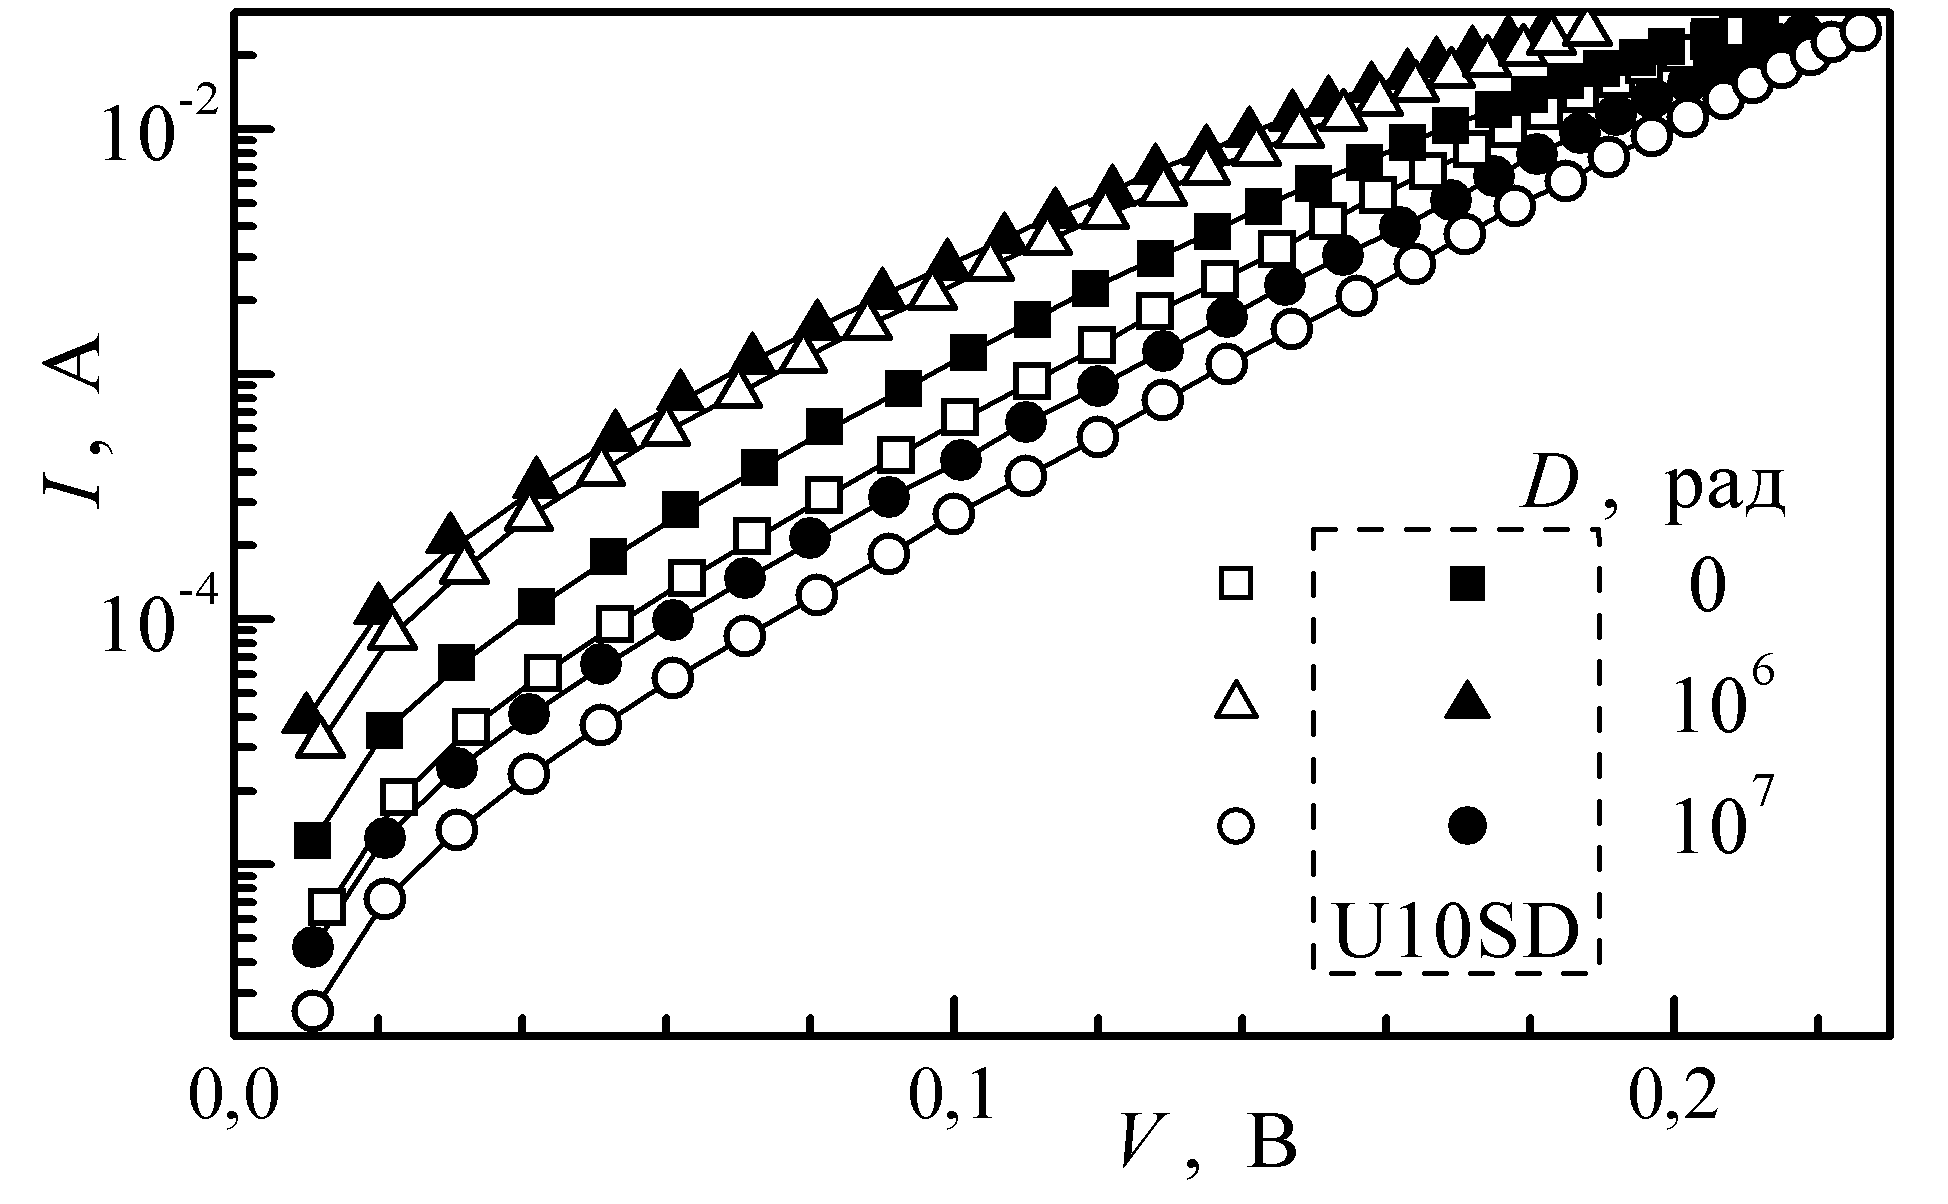
\includegraphics[width=0.7\textwidth]{figIVUSL_SDA}
\caption{\label{figIVUSL_SDA}
Прямі  ВАХ  структур SSDA (квадрати), g6SSDA (трикутники) та g7SSDA (кола), виміряні при $T=305$~K.
Заповнені та порожні точки відповідають вимірам за умов УЗН та без нього, відповідно.
$W_\mathtt{US}$, Вт/см$^2$: 0,7 (SSDA), 1,3 (g6SSDA), 1,1 (g7SSDA).
Лінії --- апроксимація відповідно до формули (\ref{eqSDA_IV}).
}%
\end{figure}

За методикою, стандартною для даного розділу, були визначені характеристики ДШ в умовах поширення акустичних коливань різної інтенсивності.
Зауважимо, що так як температура УЗН була близька до кімнатної, то в цьому випадку внесок НТКС знехтувано малий.
Еволюція величин ВБШ та фактору неідеальності представлена на На Рис.~\ref{figFbUSL_SDA}.
Дані на рисунку дозволяють виділити наступні особливості  впливу УЗ на характеристики структури металл--кремній:
\begin{enumerate}[label=\asbuk*),leftmargin=0em,itemindent=1.5em]
\item УЗН викликає зменшення ВБШ;

\item залежність зміни висоти бар'єру від $W_\mathtt{US}$ в неопромінених структурах має пороговий характер:
     величина $\Phi_b$ залишається практично незмінною поки \mbox{$W_\mathtt{US}<0,4$~Вт/см$^2$}, після чого
    зменшення ВБШ досягає $(13\pm4)$~мВ при $W_\mathtt{US}\simeq0,7$~Вт/см$^2$;

\item на відміну від ефектів, виявлених при розгляді АДВ в КСЕ (параграфи \ref{sbNIsc} та \ref{sBulyrMethod}), збільшення частоти УЗН неопромінених структур не спричинює
підвищення ефективності впливу УЗН;

\item після $\gamma$--опромінення ефективність впливу УЗН на ВБШ знижується:
абсолютне значення $\Delta\Phi_b$ не перевищує $10$~мВ для g7SSDA та $3$~мв  для g6SSDA при $W_\mathtt{US}>1$~Вт/см$^2$;

\item на залежность $\Phi_b$ від $W_\mathtt{US}$ для радіаційно модифікованих структур поріг не спостерігається;

\item збільшення поглинутої дози призводить збільшення змін ВБШ при УЗН;

\item незначні АІ зміни фактору неідеальності спостерігаються у випадку, коли $n_\mathtt{id}>1,1$ (зразок g6SSDA);
    у випадку, коли $n_\mathtt{id}$ близький до одиниці, в умовах УЗН його величина практично не міняється (зразки SSDA та g7SSDA).
\end{enumerate}

\begin{figure}
\center
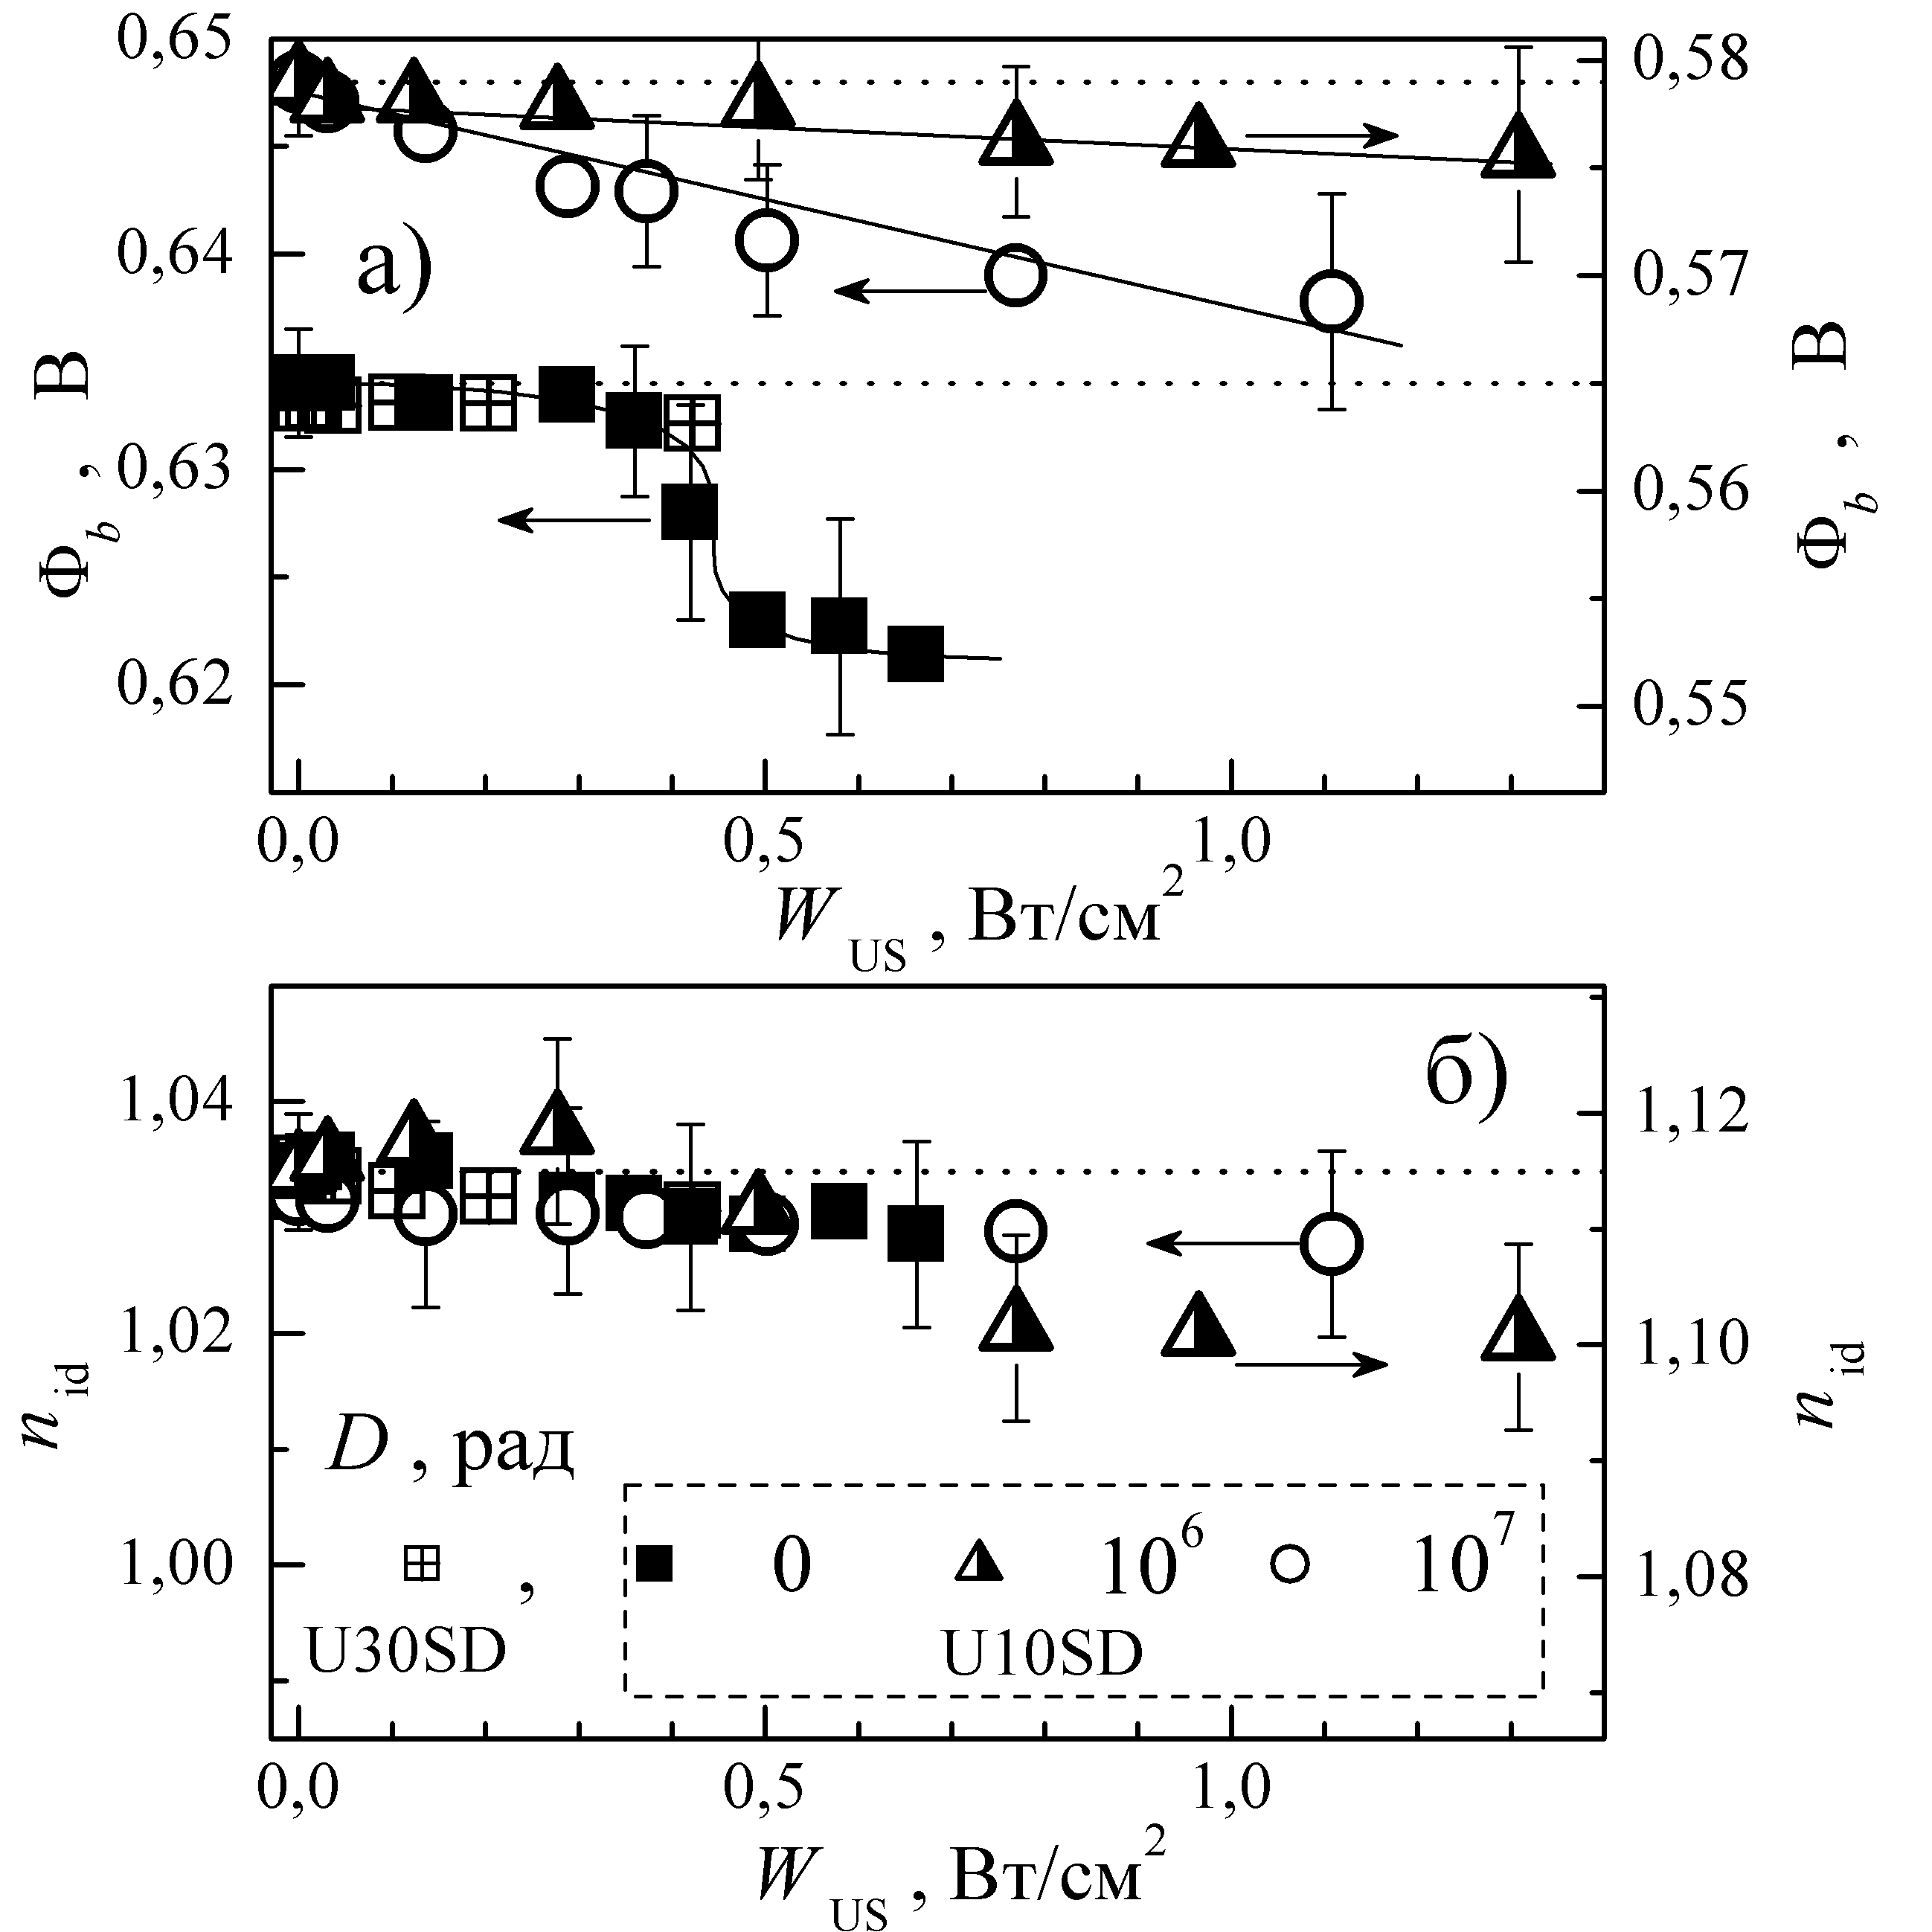
\includegraphics[width=0.7\textwidth]{figFbUSL_SDA}
\caption{\label{figFbUSL_SDA}
Залежності висоти бар'єру Шотки (а) та фактору неідеальності (б)  від інтенсивності УЗ для
структур SSDA (квадрати, праві вертикальні осі), g6SSDA (трикутники, ліві осі) та g7SSDA (кола, праві осі), виміряні при $T=305$~K.
$f_\mathtt{US}$, МГц: 9,6 (SSDA, g6SSDA, g7SSDA), 30,1 (SSDA).
Горизонтальні пунктирні лінії відповідають значенням параметрів, виміряних без УЗН.
}%
\end{figure}

Згідно з (\ref{eqFb0T}), причиною АІ змін ВБШ може бути вплив УЗ на $\Phi_b^0$ або на $\sigma_{\Phi0}$ (або й, звичайно, на обидві величини).
В свою чергу, рівняння  (\ref{eqN_T:TE}), (\ref{eqFb0T}) та (\ref{eqN_T0}) дозволяють оцінити, яким чином повинен був би змінюватись фактор неідеальності,
якби причиною зміни ВБШ були б зміни лише одного параметру з пари $(\Phi_b^0;\:\sigma_{\Phi0})$ , тоді як інший залишався би постійним.
Дійсно, при $\Phi_b^0=const$
\begin{eqnarray*}
  \Delta \Phi_b (\Phi_b^0=const)&=& \Phi_{b,in}-\Phi_{b,\mathtt{US}}=\Phi_b^0-\frac{q\sigma^2_{\Phi0,in}}{2kT}-\Phi_b^0+\frac{q\sigma^2_{\Phi0,\mathtt{US}}}{2kT}= \\
   &=&\frac{q\left(\sigma^2_{\Phi0,\mathtt{US}}-\sigma^2_{\Phi0,in}\right)}{2kT}, \\
   V_{bb,in}&=&V_{bb,\mathtt{US}},
\end{eqnarray*}
\begin{eqnarray*}
  \Delta n_{\mathrm{id}} (\Phi_b^0=const)&=&1+\frac{q\sigma_{\Phi0,in}^2}{3kV_{bb}T}-1-\frac{q\sigma_{\Phi0,\mathtt{US}}^2}{3kV_{bb}T}=\\
  &=&\frac{q\left(\sigma^2_{\Phi0,in}-\sigma^2_{\Phi0,\mathtt{US}}\right)}{3kV_{bb}T}=-\frac{2\Delta \Phi_b}{3V_{bb}}.
\end{eqnarray*}
Якщо ж незмінним залишається стандартне відхилення висоти бар'єру, то
\begin{eqnarray*}
  \Delta \Phi_b (\sigma_{\Phi0}=const)&=&\Phi_{b,in}^0-\Phi_{b,\mathtt{US}}^0,\\
  V_{bb,in}-V_{bb,\mathtt{US}}&=&\Delta \Phi_b,
\end{eqnarray*}
\begin{eqnarray*}
  \Delta n_{\mathrm{id}} (\sigma_{\Phi0}=const)&=&\frac{q\sigma_{\Phi0}^2}{3kV_{bb,in}T}-\frac{q\sigma_{\Phi0}^2}{3kV_{bb,\mathtt{US}}T}=\\
  &=&-\frac{q\sigma_{\Phi0}^2\Delta \Phi_b}{3kT\,V_{bb,in}(V_{bb,in}-\Delta \Phi_b)}.
\end{eqnarray*}
Розрахунки, проведені з використанням величини $\Delta \Phi_b=0,013$~мВ (випадок U10SD, максимальна інтенсивність) та даних Таблиці~\ref{tabPar:SSDA},
показують, що очікувані зміни фактору неідеальності $\Delta n_{\mathrm{id}} (\Phi_b^0=const)\approx-0,02$ та \mbox{$\Delta n_{\mathrm{id}}(\sigma_{\Phi0}=const)\approx-0.003$}.
До експериментальних результатів набагато ближче друге значення, тому причиною АІ зміни ВБШ є зменшення $\Phi_b^0$.

Для ідеальної структури МН в наближенні Шотки--Мота ВБШ визначається різницею між роботою виходу з металу та електронною спорідненістю напівпровідника.
Для реальних структур на інтерфейсній границі наявні електронні стані, енергія яких відповідає забороненій зоні напівпровідника;
при їх великій кількості величина ВБШ прямує до так званої границі Бардіна: $q\Phi_b^0=E_g-\varphi_0$,
де $\varphi_0$ --- рівень нейтральності інтерфейсних станів, тобто рівень, до якого всі поверхневі стани мають бути заповненими для того, щоб
поверхня була електронейтральна.
Якщо густина інтерфейсних станів $D_{ss}$ не надто велика, то значення ВБШ визначається середньозваженою величиною між цими двома
граничними випадками, причому вагові коефіцієнти залежать від $D_{ss}$.
Так як АІ ефекти є оборотними, то їх не можна пов'язати зі зміною кількості станів.
Отже, причиною зменшення ВБШ при УЗН найбільш ймовірно є зміна $\varphi_0$ внаслідок, наприклад, АІ іонізації дефектів на границі розділу.
В неопромінених структурах іонізація відбувається внаслідок коливання дислокацій, наявність яких у подібних структурах вже обговорювалася вище.
В рамках такого припущення знаходять пояснення пороговий характер та частотна незалежність змін $\Phi_b$:
ефективність коливань дислокаційних відрізків суттєво збільшується при їх відриві від стопорів і для використаного частотного діапазону
практично не залежить від періоду коливань.
Зауважимо, що ефекти АІ іонізації дефектів, в тому числі і дислокацій на границі бар'єрних структур, спостерігалися і раніше \cite{Olikh:FTP2011,Korotchenkov1995,OstrKorBook}.


Внаслідок $\gamma$--опромінення механізм впливу УЗ змінюється.
Гетерування РД в області дислокацій викликає закріпленні останніх, як наслідок, лінійні дефекти нездатні ефективно взаємодіяти з АХ при тих самих значеннях
$W_\mathtt{US}$, як і до опромінення.
З іншого боку, точкові радіаційні дефекти на кшталт дивакансій чи А--центрів у $\gamma$--опроміненому кремнії є акустоактивними --- див. розділ~\ref{Ch_SSC}, роботу \cite{YOlikh2006TPLr}.
Якщо зменшення ВБШ в g6SSDA та g7SSDA відбувається внаслідок іонізації точкових РД, то повинно відбуватися підсилення АІ ефектів зі збільшенням поглинутої дози.
Саме це і спостерігається на експерименті --- див. Рис.~\ref{figFbUSL_SDA},а.
Крім того, в опромінених структурах УЗ здатен впливати та стан патчів внаслідок взаємодії з РД, захопленими в областях неоднорідності.
Це знаходить свій прояв у АІ зміні фактора неідеальності структур g6SSDA, для яких, як було показано вище, вплив неоднорідностей на перенесення заряду при прямому зміщенні достатньо великий.
При збільшенні дози, коли модель ТЕ через неоднорідний контакт перестає бути застосовною, зникають і ефекти впливу УЗ на $n_\mathtt{id}$.


\subsection{Особливості поведінки тунельної та термоемісійного компонент зворотного струму в умовах ультразвукового навантаження}

На Рис.~\ref{figIVrg0USL_SDA} показано зворотні гілки ВАХ структур Al$-n-n^+$--Si---Al, виміряні при УЗН та для ненавантажених
зразків при однакових температурах.
З рисунку видно, що спостерігається АІ збільшення величини $I_R$ незалежно від ступеню опромінення, проте з підвищенням зворотного
зміщення ці ефекти послаблюються.
Крім цього, на рисунку показані польові залежності внесків термоемісійної, температуро--незалежної та тунельно--багатофононної компонент
зворотного струму в околі кімнатних температур.
Максимальні зміни $I_R$ спостерігаються при зміщеннях, коли переважаючим є ТЕ струм.


\begin{figure}
\center
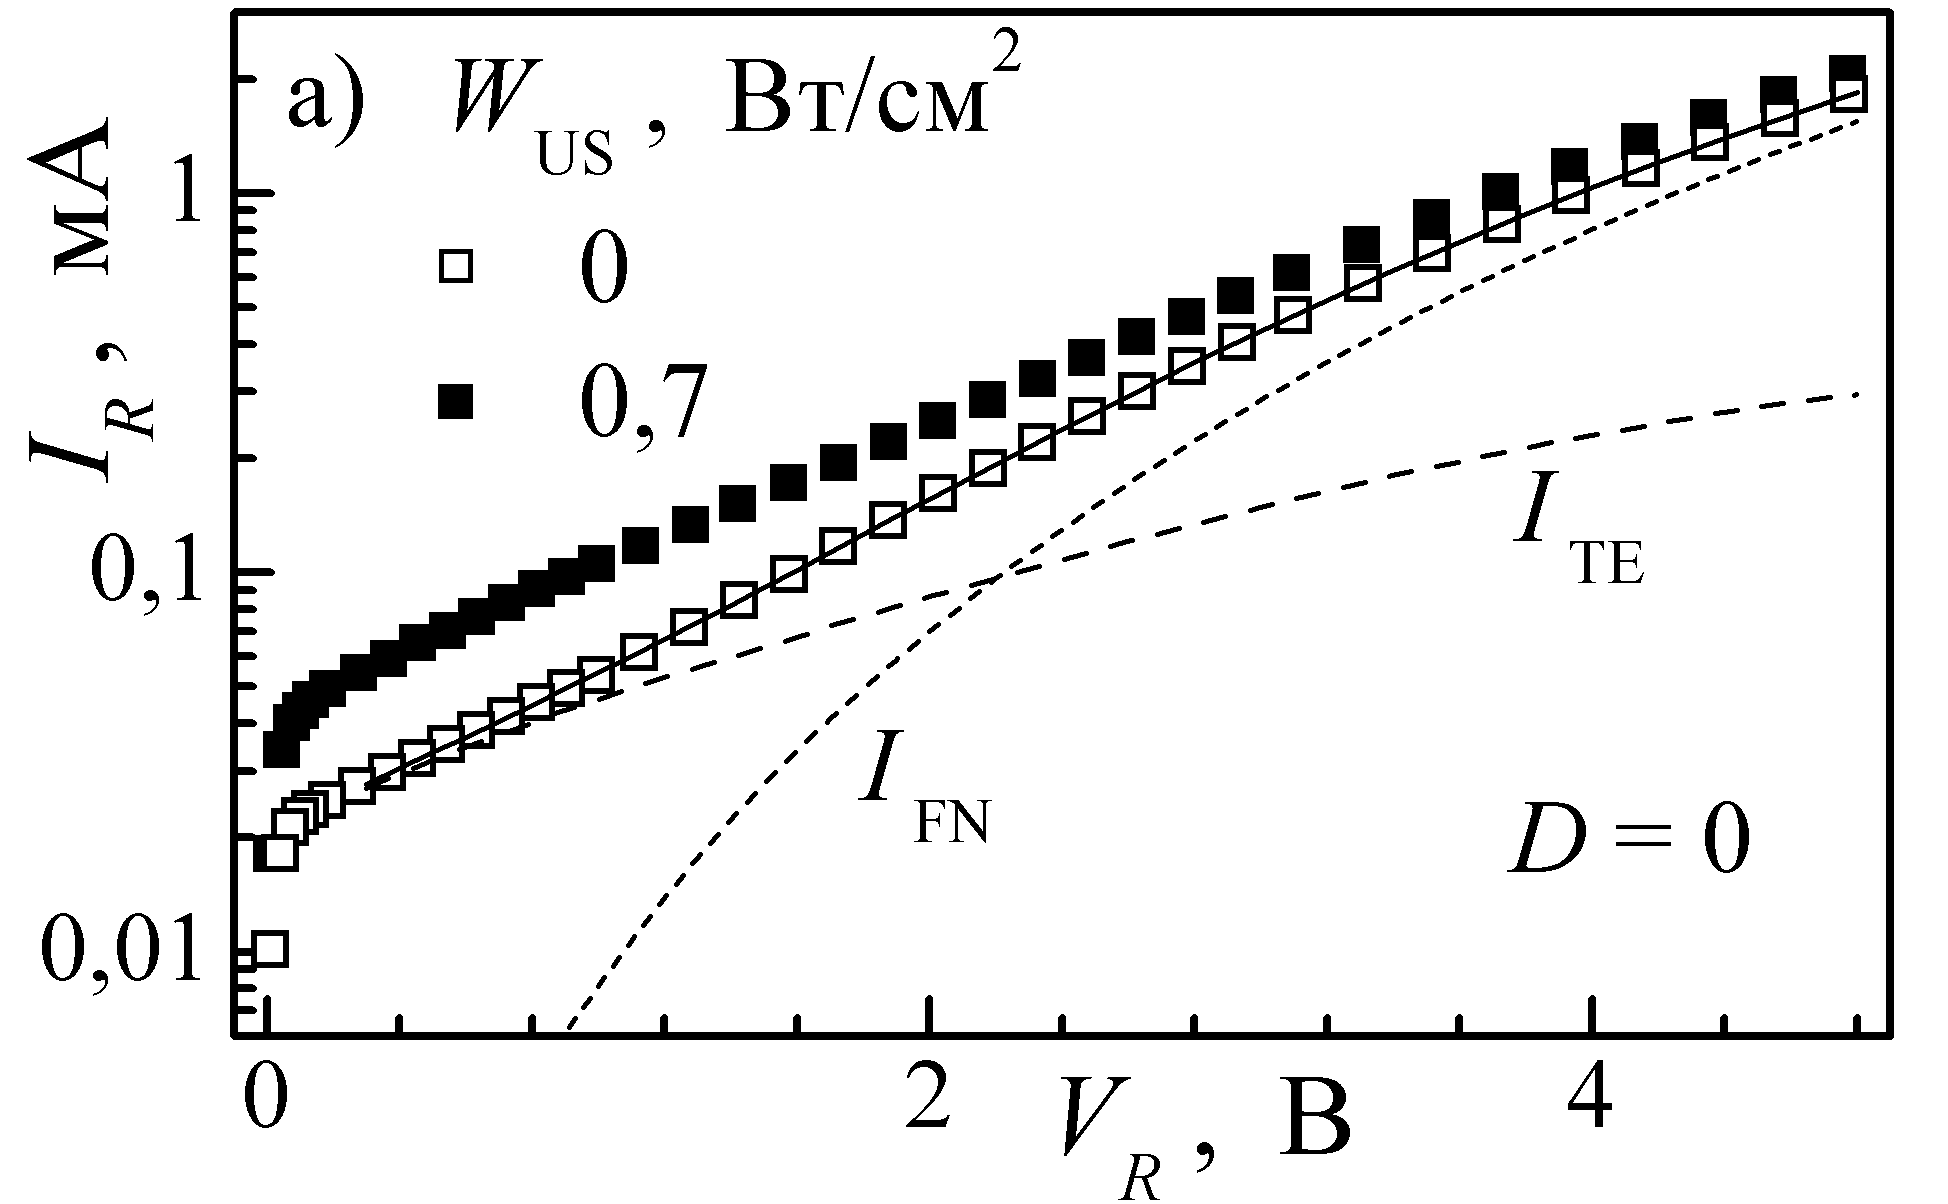
\includegraphics[width=0.55\textwidth]{figIVrg0USL_SDA}
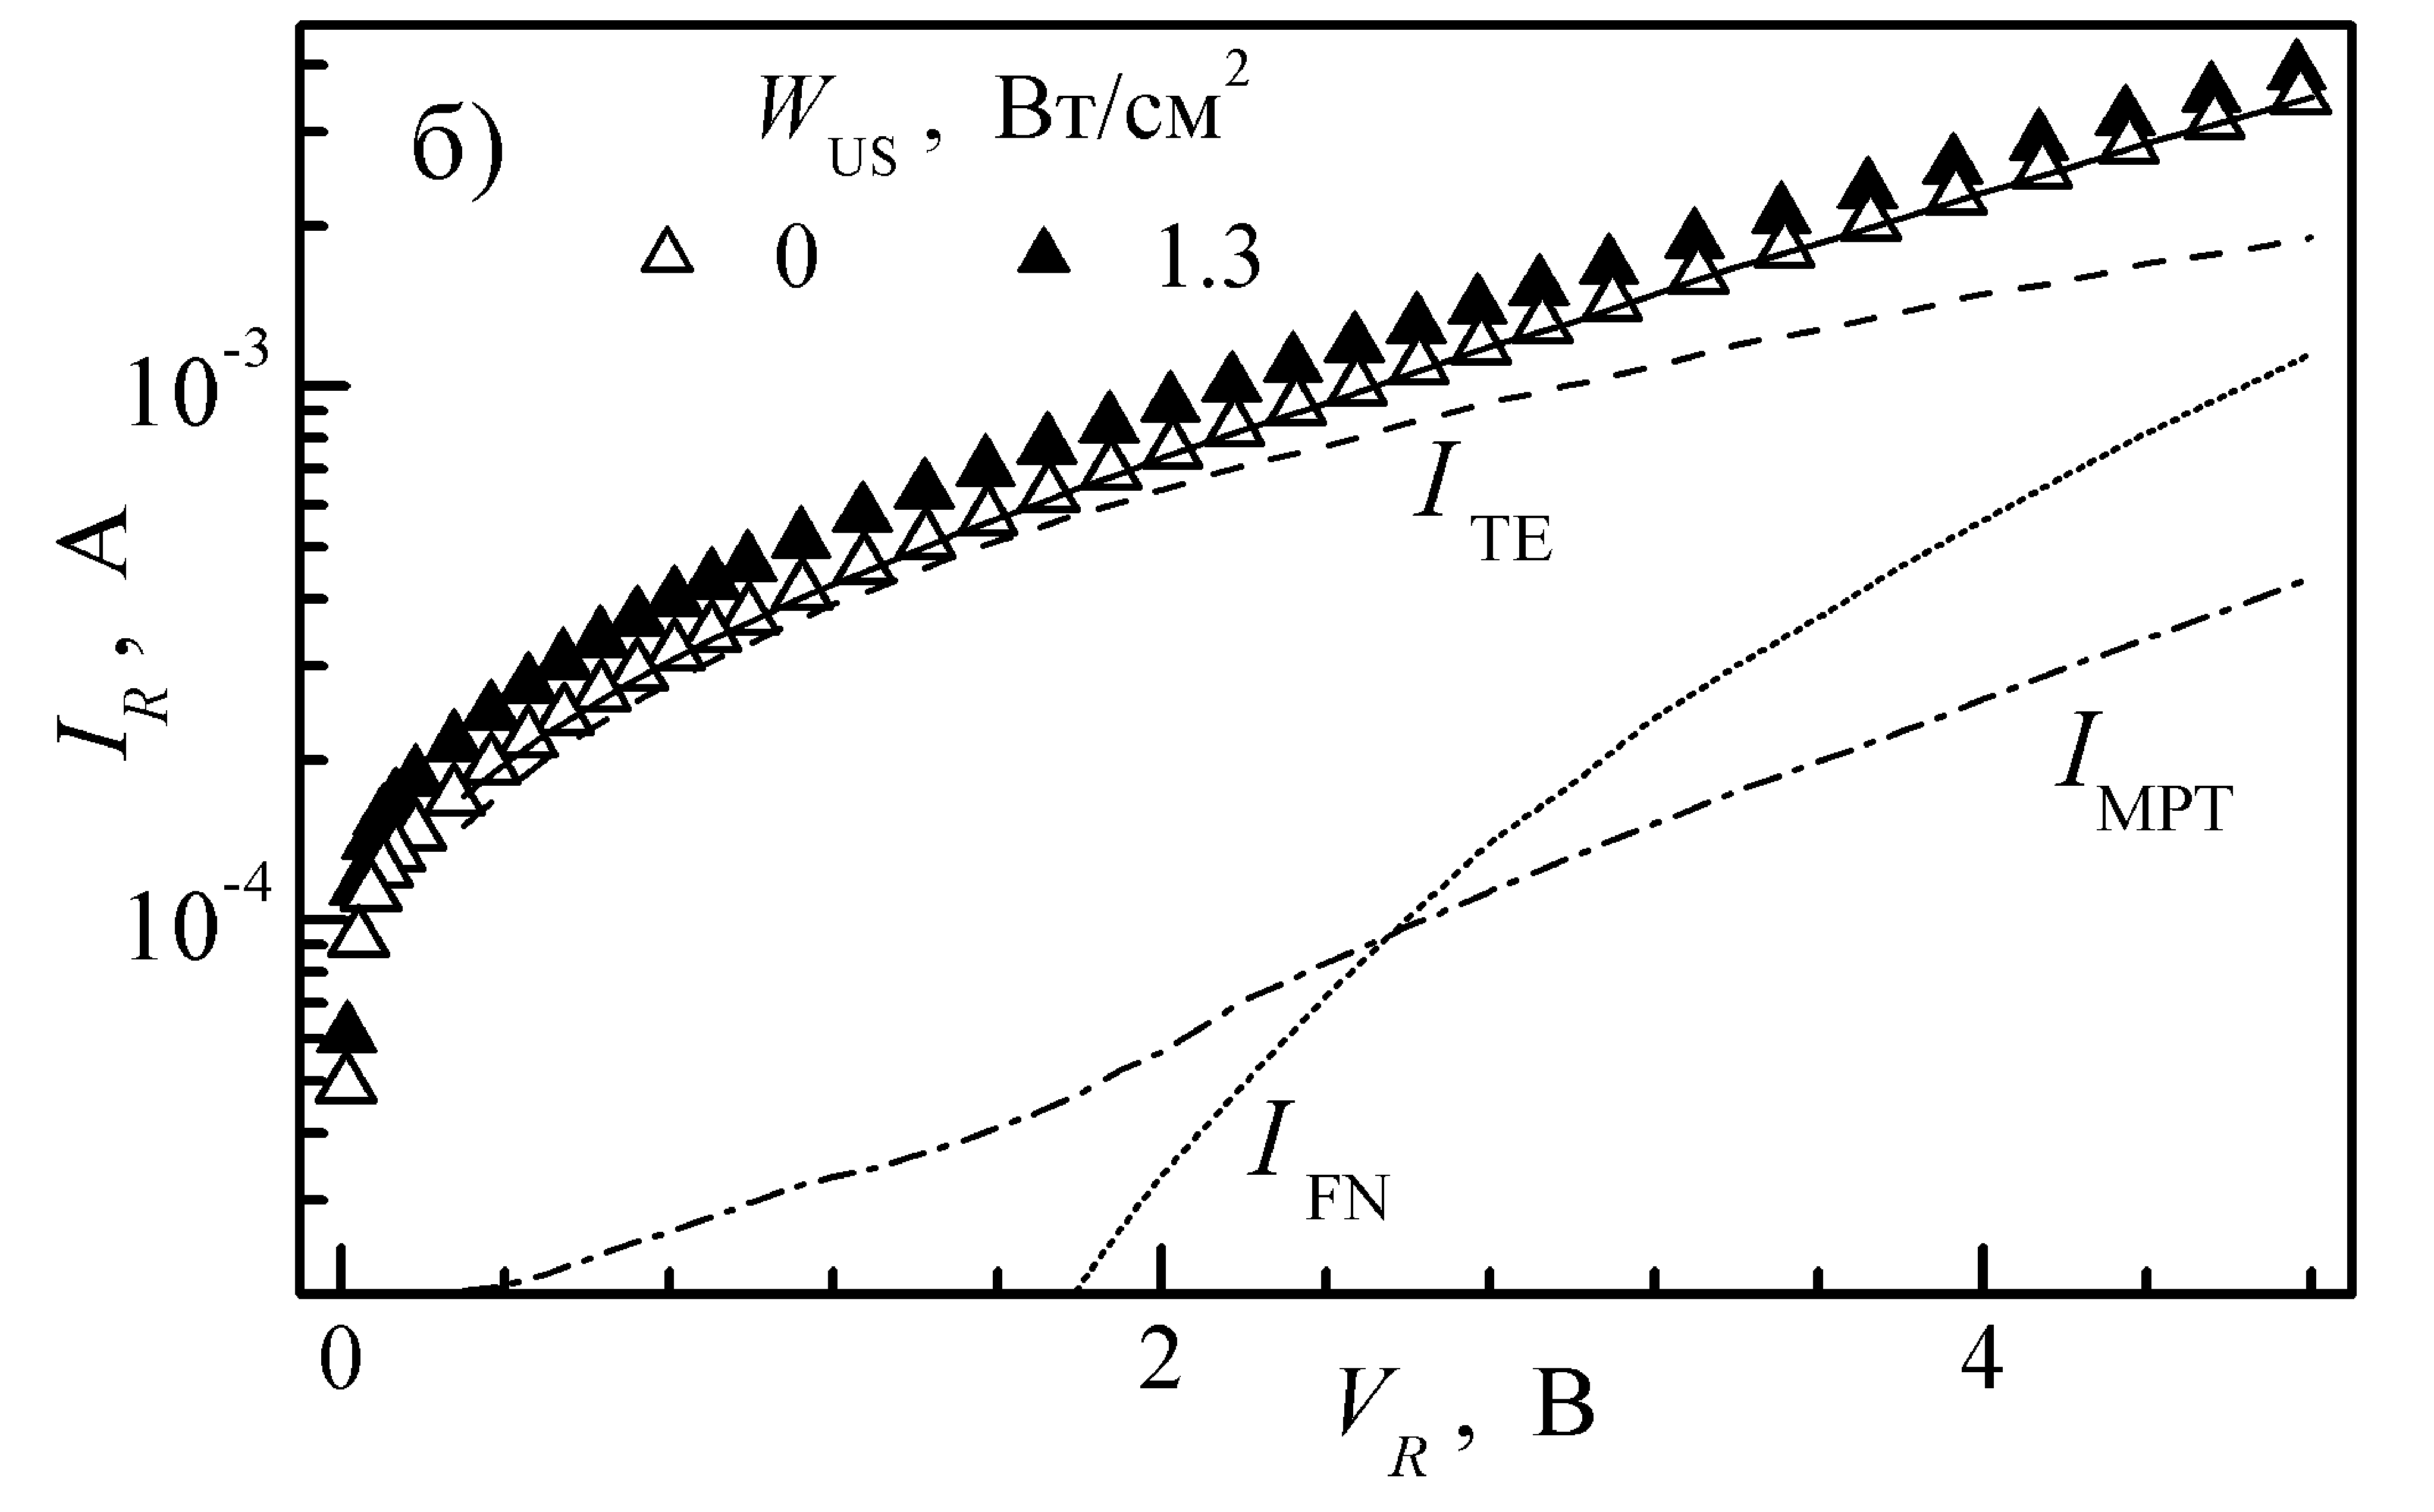
\includegraphics[width=0.55\textwidth]{figIVrg6USL_SDA}
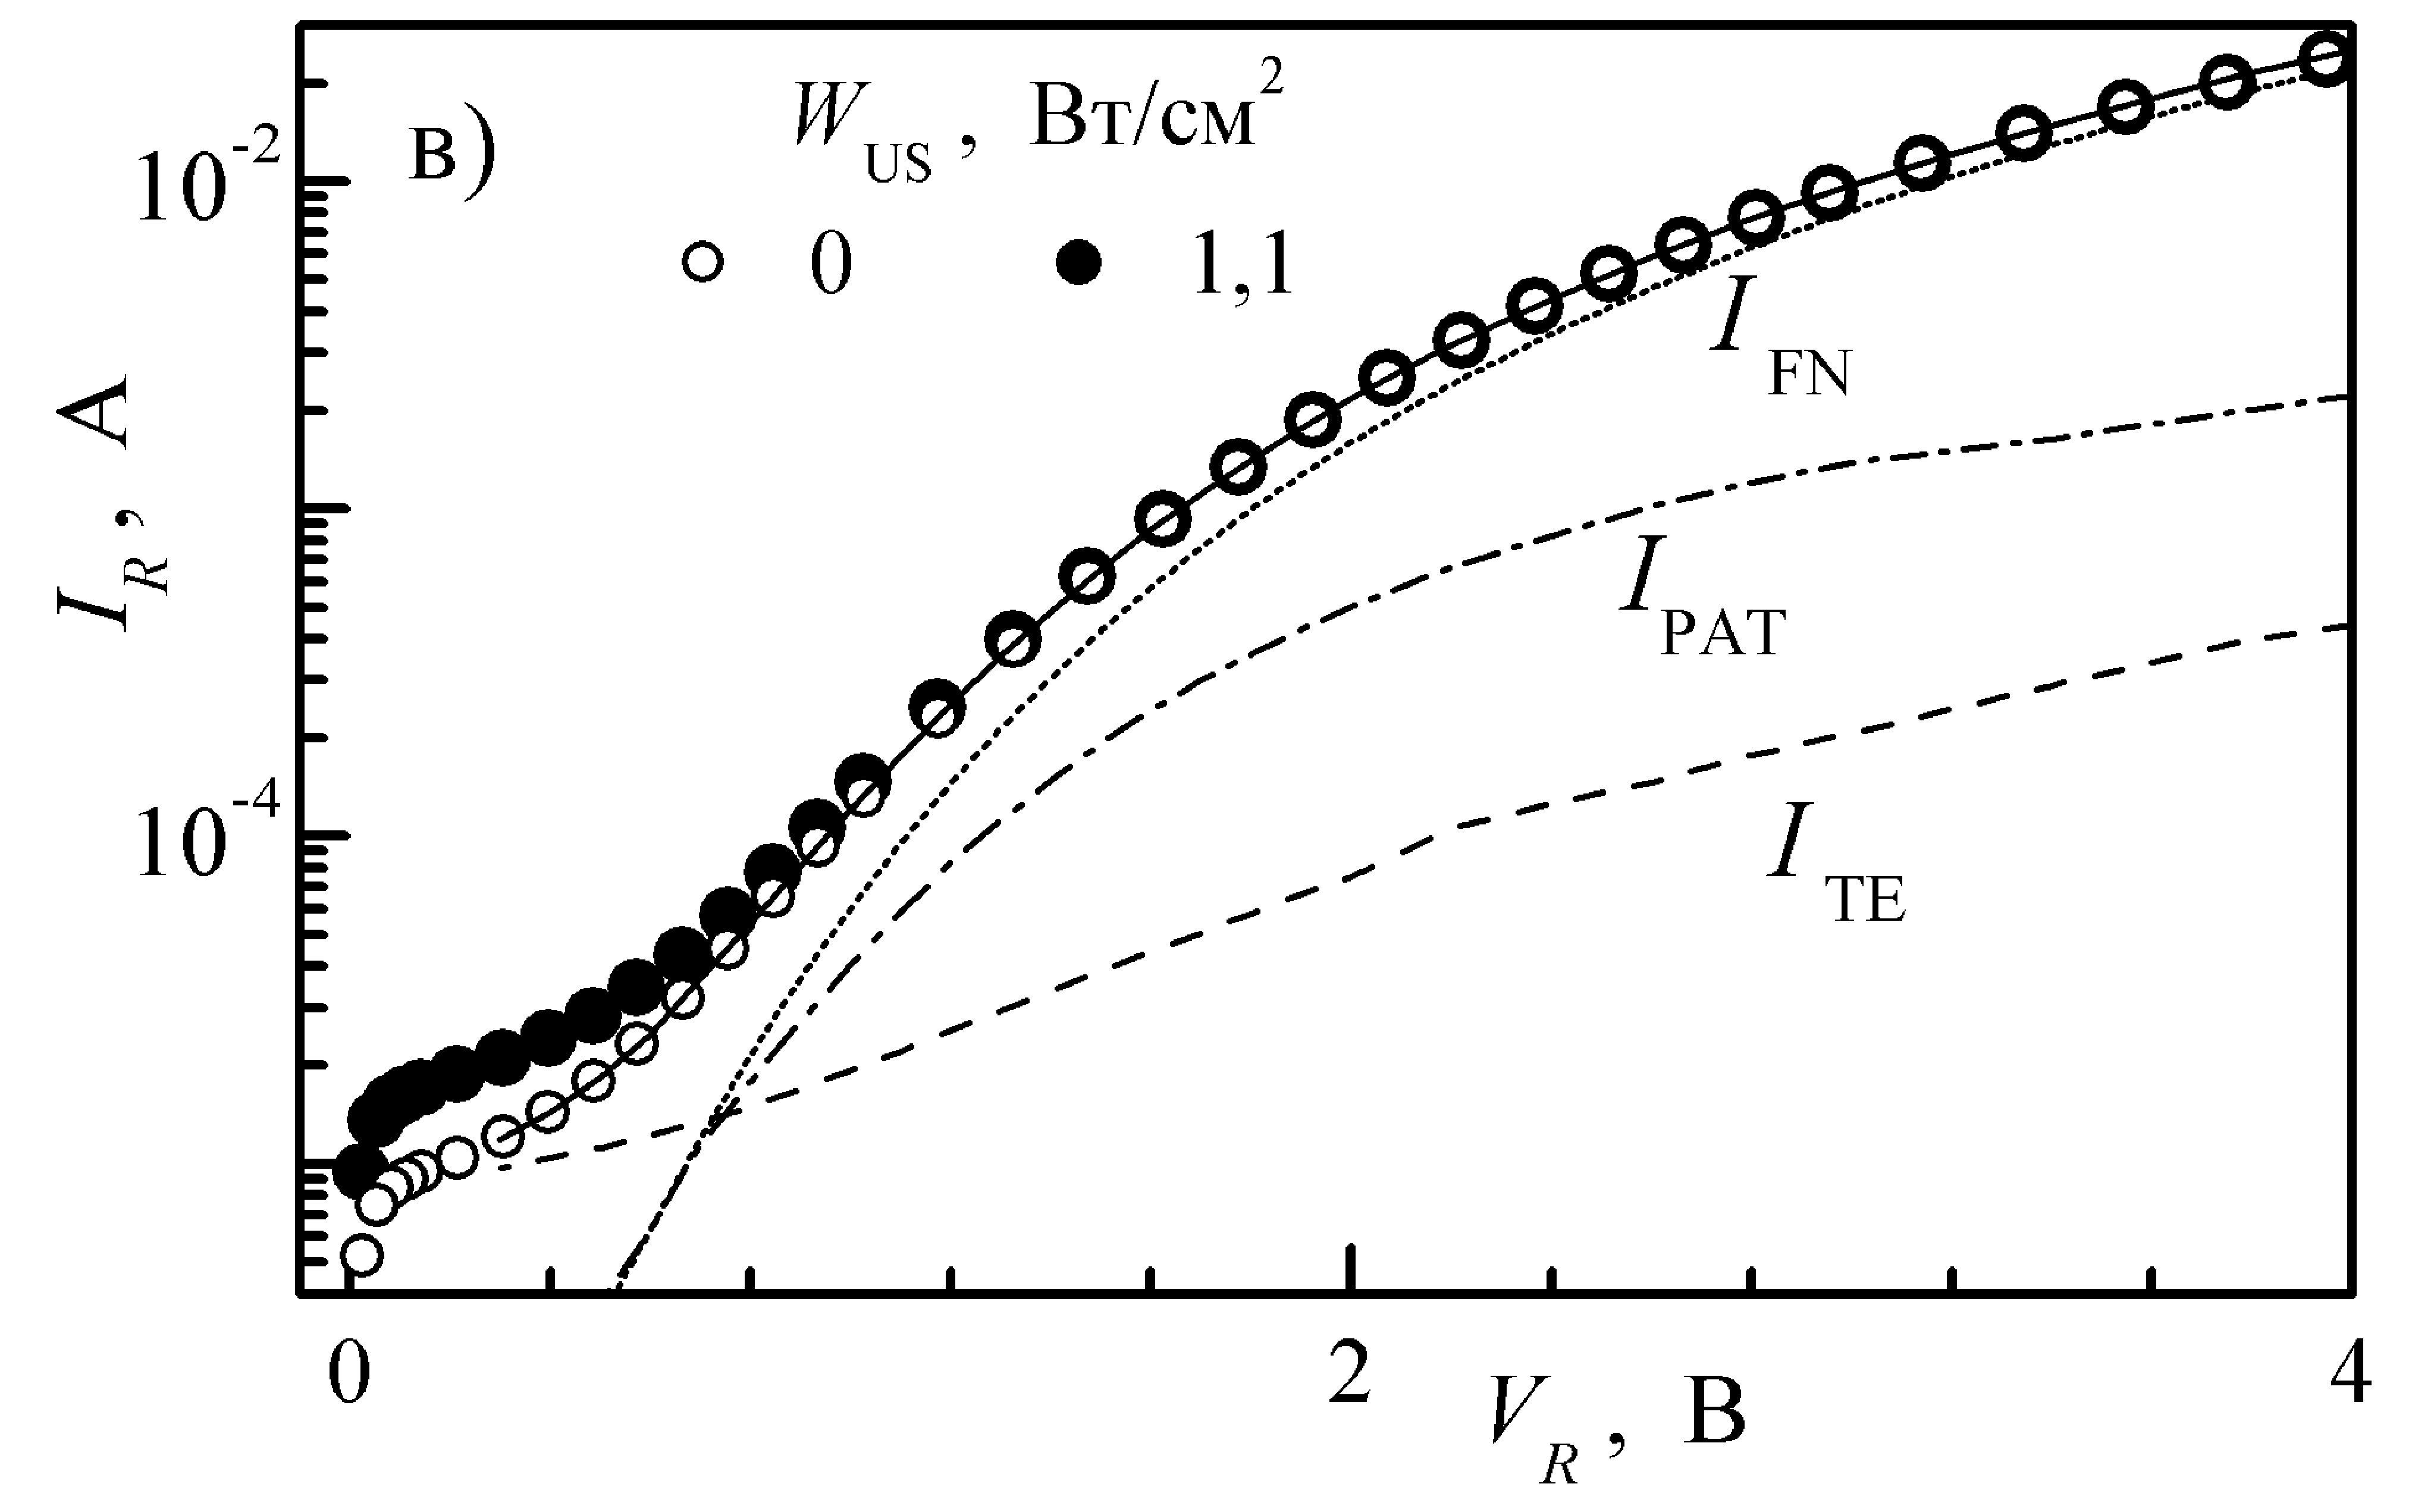
\includegraphics[width=0.55\textwidth]{figIVrg7USL_SDA}
\caption{\label{figIVrg0USL_SDA}
Зворотні  ВАХ  структур SSDA (а), g6SSDA (б) та g7SSDA (в), виміряні при $T=305$~K.
Заповнені та порожні точки відповідають вимірам за умов УЗН та без нього, відповідно.
$f_\mathtt{US}=9,6$~МГц.
Суцільні лінії --- апроксимація відповідно до формули (\ref{eqIrRad}),
розривні відображають окремі складові зворотного струму для ненавантажених структур.
}%
\end{figure}



На Рис.~\ref{figeIrWus_SDA} наведено типові амплітудні залежності величини відносних АІ змін зворотного струму.
Зауважимо, що на рисунку для зручності наведено залежність модуля $\varepsilon_{IR}$, так як при зростанні струму результати обчислення згідно з виразом~(\ref{eqEpsDelta}) від'ємні.
Видно, що
а)~збільшення $I_R$ може досягати декількох десятків відсотків;
б)~в неопромінених структурах на амплітудній залежності спостерігається певний поріг, що відповідає $W_\mathtt{US}\approx0,4$~Вт/см$^2$;
в)~після опромінення спостерігається як зменшення ефективності впливу УЗН, так і зникнення порогу;
г)~АІ зміни зворотного струму зростають з підвищенням поглинутої дози.


\begin{figure}
\center
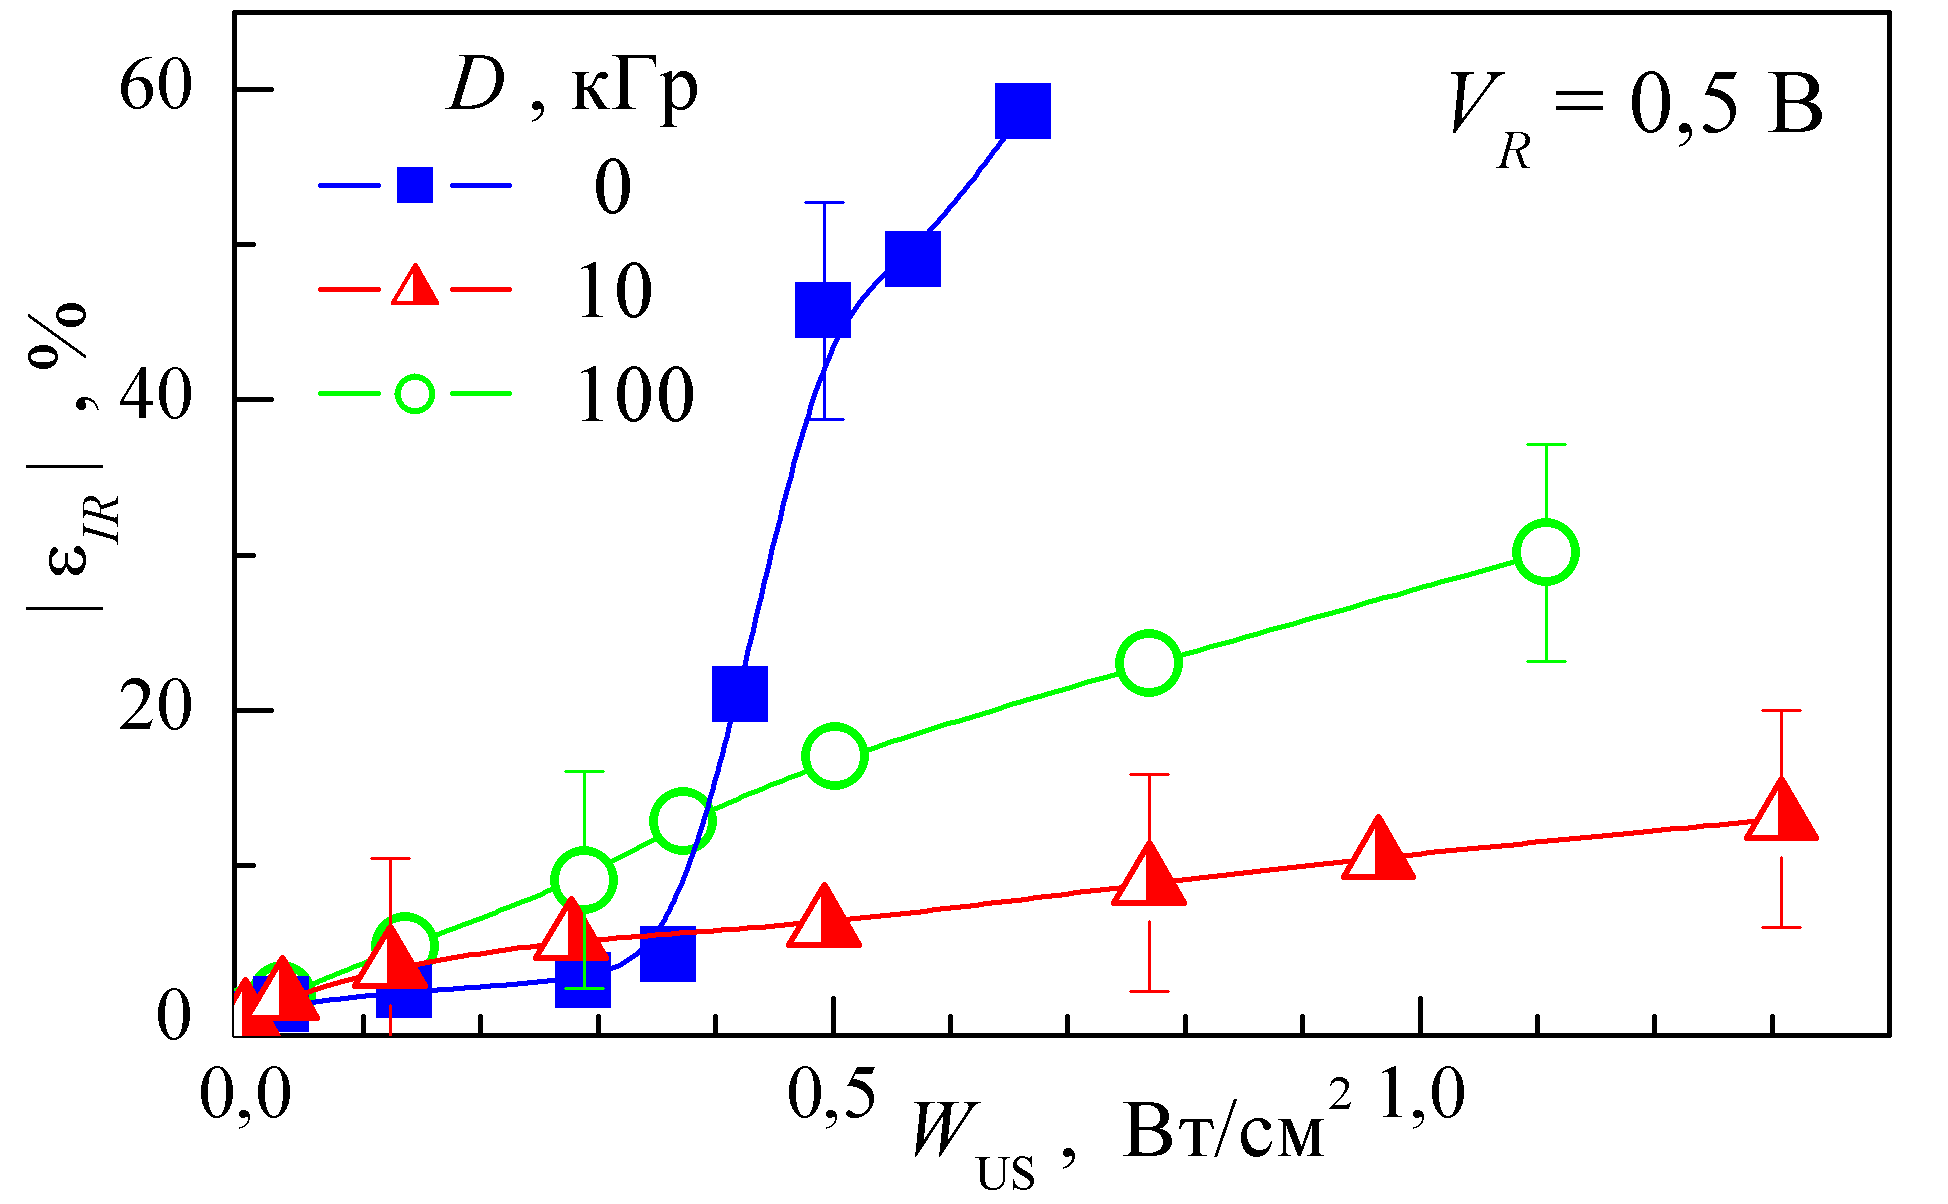
\includegraphics[width=0.65\textwidth]{figeIrWus_SDA}
\caption{\label{figeIrWus_SDA}
Залежності АІ відносних змін зворотного струму від інтенсивності УЗ.
$f_\mathtt{US}=9,6$~МГц.
$V_R=0.5$~B. $T=305$~K.
Точки --- експеримент,
лінії наведено для зручності.
}%
\end{figure}

Такі особливості акустичного впливу дозволяють запропонувати метод оцінки дози $\gamma$--квантів, поглинутих структурою МН.
А саме, метод може базуватися на вимірюванні АІ зміни величини зворотного струму $\varepsilon_{IR}$ хоча б при двох значеннях $W_\mathtt{US}$,
одне з яких більше, а інше менше порогу для неопроміненого зразка.
Відношення отриманих величин дозволить зробити висновок про сам факт опромінення,
а безпосереднє значення $\varepsilon_{IR}$ при більшій інтенсивності УЗ пов’язана з дозою.
Подібна система ДШ--п’єзоперетворювач може бути своєрідним сенсором $\gamma$--опромінення.

Дані на Рис.~\ref{figeIrVrUSL_SDA} дозволяють детально порівняти залежності відносних внесків кожної з компонент зворотного струму від прикладеної напруги
як для неопромінених, так і опромінених структур з відповідними залежностями АІ змін загального $I_R$.
Видно, що незалежно від ступеню опромінення характер польових залежностей АІ змін зворотного струму співпадає з поведінкою термоемісійної складової.


\begin{figure}
\center
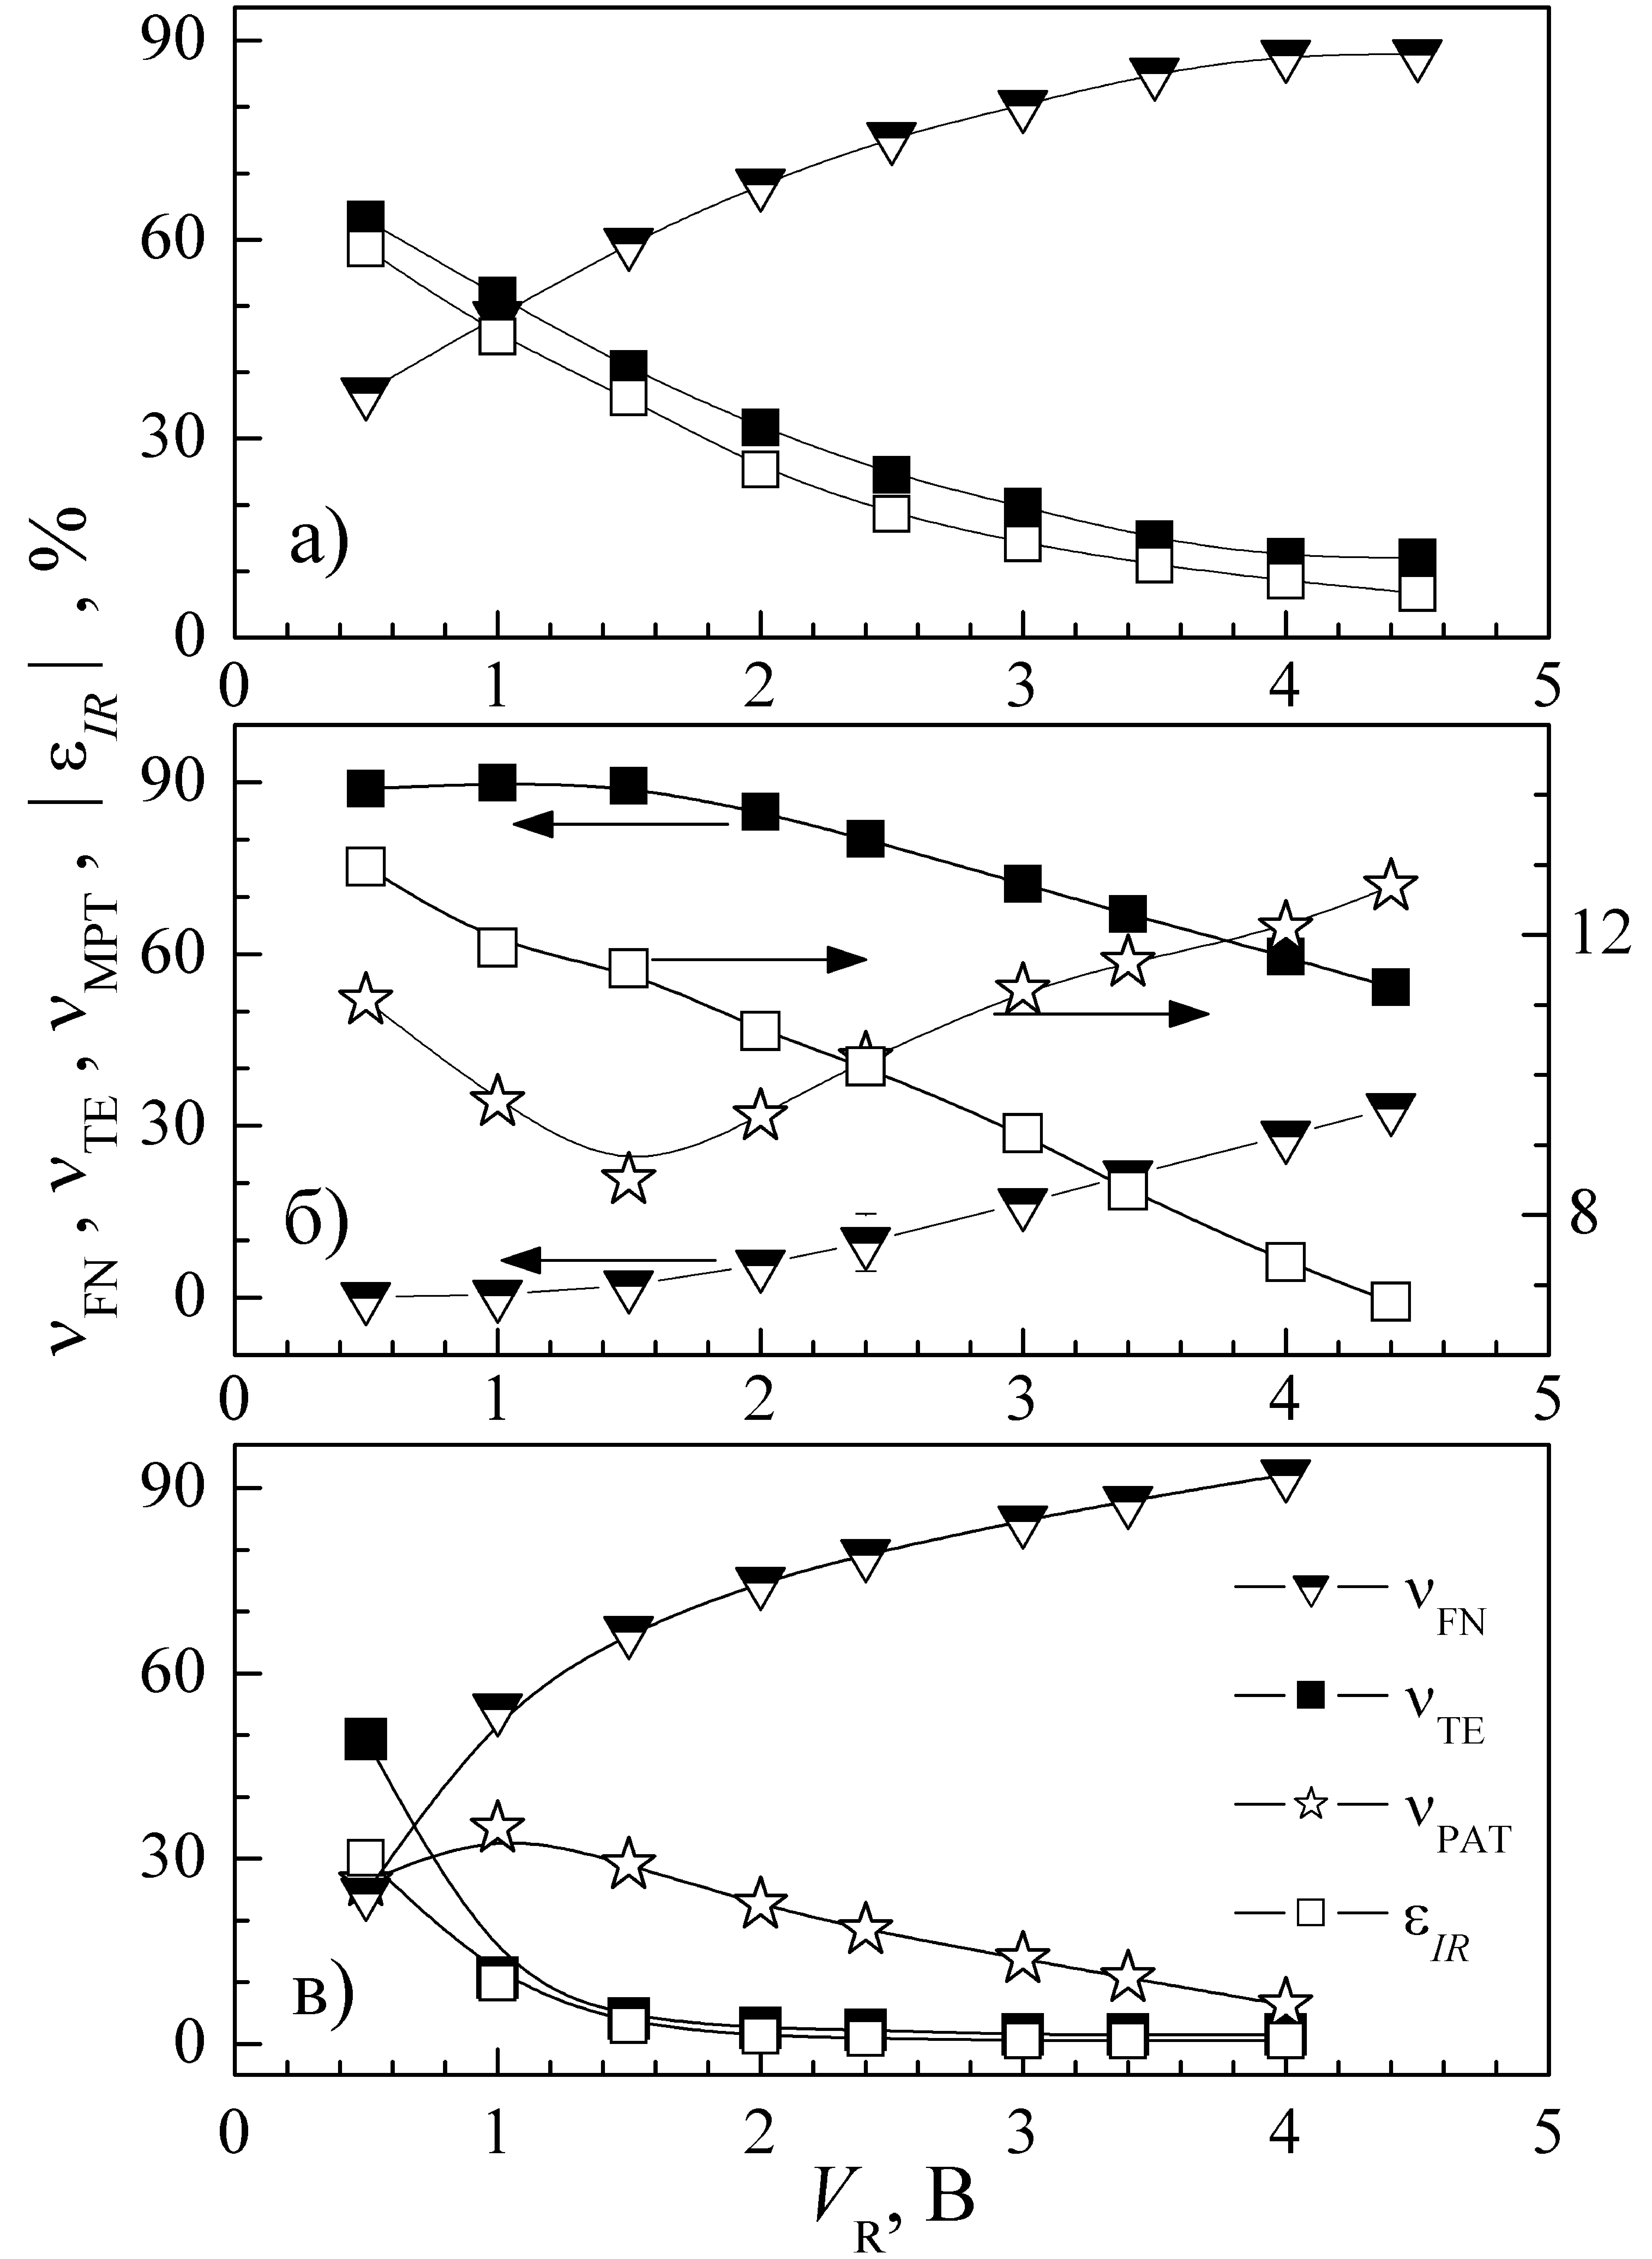
\includegraphics[width=0.5\textwidth]{figeIrVrUSL_SDA}
\caption{\label{figeIrVrUSL_SDA}
Залежності відносних внесків окремих компонент у загальний зворотний струм
та відносної АІ зміни зворотного струму від напруги зміщення.
$D$, рад: 0 (a), $10^6$ (б), $10^7$ (в).
$W_\mathtt{US}$, Вт/см$^2$: 0,6 (а), 1,3 (б), 1,1 (в).
$f_\mathtt{US}=9,6$~МГц.
$T=305$~K.
Точки --- експеримент,
лінії наведено для зручності.
}%
\end{figure}


Весь масив представлених результатів свідчить на користь того, що
динамічні зміни зворотного струму як $\gamma$--опромінених, так і неопромінених структур Al$-n-n^+$--Si---Al в умовах УЗН
пов’язані з впливом пружних коливань на термоемісійні процеси і пояснюються зменшенням ВБШ, детально розглянутим у попередньому параграфі.
З іншого боку, відсутність впливу УЗН на складові струму, пов’язані з прямим та багатофононним тунелюваннями за участю глибоких центрів,
свідчить про те, що відповідні дефекти не є акустоактивними.
Зокрема, центр з енергією іонізації $0.12$~еВ (С$_i$) не приймає участь у АДВ.
Нагадаємо, що результати досліджень КСЕ (параграф \ref{sbRadDef}) показали, що не АА є і інший дефект, який містить міжвузольний атом вуглецю, C$_i$O$_i$.

Відсутність впливу УЗН на тунельну складову струму свідчить про вибірковості акустичного впливу, яка не характерна для більш традиційних методів модифікації параметрів напівпровідникових структур.
Наприклад, в результаті іонного або електронного опромінення структур з бар'єром Шотки на основі $n$-Si відбувається збільшення зворотного струму
і зменшення $\Phi_b$,
проте поява радіаційних дефектів інтенсифікує і процеси тунелювання \cite{Kumar2,Rao,SINGH2001}.
Отже, УЗ може бути інструментом цілеспрямованого впливу на певні параметри структур метал--напівпровідник.


%\cite{Vorobets:FM2003,StrihaBook1987,VOROBETS2005,Vorobets}
%
%FTP
%\cite{Evtuh,Kumar2,Rao,SINGH2001}
%
%IEEE
%\cite{Roul,Novikov,Yu,Andrews,Shcherb,Muzafarova,Belyaev,Boltovets}
%
%SEMST
%\cite{Tataroglu:2009,Gullu:2008,Karatas:2006NIMA,Karatas:2005NIMA,Tataroglu:2007NIMA,Kinoshita,
%YOlikh2007TPLr,Parchinskii2006r,Gorb2010,YOlikh2006TPLr,Parchinskii2000r,Olikh:FTP2011,Rhoderick1988,
%Novikov,Kurnosova,Bulyarskii2001r,Vavilov1990r,Song1987,Muzafarova,Tung:PhysRev,Evstropov,Ganichev1997,Korotchenkov1995,OstrKorBook}
%
%Ultras
%\cite{Zaver:2008r}
%


\section*{Висновки до розділу \ref{Ch_GammaSD}}
\addcontentsline{toc}{section}{Висновки до розділу \ref{Ch_GammaSD}}
  \begin{enumerate}
     \item Проведено експериментальне дослідження прямих і зворотних вольт--амперних характеристик структур Al$-n-n^+$--Si---Al з бар'єром Шотки в діапазоні температур $130\div330$~К.

     \item Виявлено, що при підвищенні температури спостерігається збільшення висоти бар'єру та зменшення фактору неідеальності.
       Показано, що отримані результати можна пояснити у рамках моделі термоелектронної емісії через неоднорідний контакт у всьому діапазоні температур.
       Визначені середня висота бар'єру Шотки та її стандартне відхилення:
       $0,872\pm0,004$~В та $0,099\pm0,001$~В при $(130\div220)$~К та
       $0,663\pm0,003$~В та $0,040\pm0,005$~В при $(230\div330)$~К, відповідно.

     \item Використовуючи модифіковану залежність Річардсона визначено сталу Річардсона --- ($115\pm10$)~А$\cdot$см$^{-2}\cdot$К$^{-2}$.

     \item Показано, що при низьких температурах ($T<220$~К) суттєвим стає проходження заряду через області зі зниженим бар'єром і
           визначено середнє значення висоти бар'єру Шотки в цих областях --- $54\pm4$~мВ.

    \item Показано, що при зворотному зміщенні в структурах Al$-n-n^+$--Si---Al перенесення заряду відбувається як внаслідок
          термоелектронної емісії через неоднорідний бар'єр, так і завдяки процесам прямого тунелювання через глибокий центр,
          яким, імовірно, є міжвузольний атом вуглецю.

\item Проведено експериментальне дослідження впливу $^{60}$Co $\gamma$--ви\-про\-мі\-ню\-ван\-ня $^{60}$Co на електрофізичні параметри
     структур Al$-n-n^+$--Si---Al.
Виявлено, що висота бар'єру, фактор неідеальності та величина зворотного струму немонотонно змінюються при збільшенні поглинутої дози.

\item Показано, що радіаційне опромінення суттєво підсилює процеси тунелювання носіїв заряду як при прямому зміщенні, так і при зворотному.
     Зокрема, при прямому зміщенні тунельний механізм перенесення струму стає основним в низькотемпературній області ($T<250$~К),
а при зворотному з'являється компонента струму, пов'язана з багатофононним тунелюванням.

\item Виявлено, що причини зміни електрофізичних параметрів $\gamma$--оп\-ро\-мі\-не\-них структур різняться для низьких та високих значень поглинутої дози.
      Зокрема, при низьких дозах відбувається накопичення дефектів акцепторного типу на границі розділу
метал--напівпровідник та укрупнення патчів внаслідок радіаційно підсиленного дислокаційного ковзання.
 При великих дозах цей ефект маскується інтенсифікацією процесів тунелювання внаслідок утворення значної кількості радіаційних дефектів.

\item Показано, що характер дозової немонотонності зміни висоти бар'єру Шотки різний для
      однорідних областей та для всього діоду загалом.

     \item Вперше експериментально досліджено вплив ультразвукового навантаження у динамічному режимі при кімнатній температурі
           на параметри кремнієвих діодів Шотки.
           Виявлено, що при поширенні акустичних хвиль спостерігаються оборотні зменшення висота бар'єру,
збільшення зворотного струму та струму насичення, в той час як фактор неідеальності практично не змінюється.

\item Встановлено, що зміни зворотнього струму та висоти бар'єру в $\gamma$--опромінених кремнієвих структурах практично лінійно залежать від інтенсивності УЗ,
    тоді як в неопромінених діодах Шотки ця залежність має пороговий характер.

    \item Виявлено, що ультразвукове навантаження практично не впливає на процеси прямого тунелювання та багатофононного тунелювання;
     центр з енергією активації $0.12$~еВ не є акустоактивним.

\item Показано, що вплив збільшення термоемісійної складової струму (і прямого, і зворотного) в умовах акустичного навантаження структур можна пояснити іонізацією дефектів, що знаходяться на границі розділу,
  внаслідок взаємодії ультразвуку з дислокаціями та радіаційними точковими порушеннями періодичності в неопромінених та опромінених структурах, відповідно.

  \end{enumerate}	

Основні результати даного розділу представлені в роботах \cite{Olikh:2013IEEE,Olikh:UPJ2013,Olikh:FTP2013,Olikh:SEMT2013,
Olikh:Ultras,7Drog,5UNCPS,2012Ternop,14Plivk,6UNCPS,2014IUS}.
